\documentclass[10pt,letterpaper]{article}

\usepackage[margin=0.84in,top=0.86in,bottom=0.86in,headheight=19pt,headsep=14pt]{geometry}
\usepackage{amsmath,amssymb,amsthm,mathtools}
\usepackage{fontspec}
\usepackage{microtype}
\usepackage{booktabs}
\usepackage{array}
\usepackage{float}
\usepackage{graphicx}
\usepackage{xcolor}
\usepackage{enumitem}
\usepackage{fancyhdr}
\usepackage[skins,breakable]{tcolorbox}
\usepackage{listings}
\usepackage[colorlinks=true,linkcolor=accentblue,citecolor=accentblue,urlcolor=accentblue,
  pdftitle={No Finite-Dimensional Extremizer for Subquadratic Lee Constants (MI-20) — Version 5: Spectral-Pencil Trace-Class Proofs, Bogomolny Identities, Universal Hirota Solitons, Zero-Float Multi-Summand Enclosures, and 73-Theorem Lean 4 Formalization},
  pdfauthor={Marcio Díaz (Space Research AI)},
  pdfsubject={Open Problem MI-20 (OpenProblemsInNLA), Matrix Analysis, Schatten Norms, Operator Inequalities, Formal Verification (Lean 4)},
  pdfkeywords={Lee conjecture, Schatten norms, quasi-reverse Minkowski inequality, MI-20, spectral pencils, Bogomolny sum-of-squares, Hirota soliton, Bernstein polynomial certificates, Lean 4, Mathlib, Space Research AI, Marcio Díaz}]{hyperref}

% Fonts (Tectonic / XeTeX bundled TeX Gyre Pagella + Heros + Cursor)
\setmainfont{texgyrepagella}[
  Extension=.otf,
  UprightFont=*-regular,
  BoldFont=*-bold,
  ItalicFont=*-italic,
  BoldItalicFont=*-bolditalic
]
\setsansfont{texgyreheros}[
  Extension=.otf,
  UprightFont=*-regular,
  BoldFont=*-bold,
  ItalicFont=*-italic,
  BoldItalicFont=*-bolditalic,
  Scale=MatchLowercase
]
\setmonofont{texgyrecursor}[
  Extension=.otf,
  UprightFont=*-regular,
  BoldFont=*-bold,
  ItalicFont=*-italic,
  BoldItalicFont=*-bolditalic,
  Scale=0.85
]

% Color palette
\definecolor{ink}{HTML}{0F2537}
\definecolor{accentblue}{HTML}{1D4ED8}
\definecolor{accentteal}{HTML}{0F766E}
\definecolor{muted}{HTML}{52606D}
\definecolor{boxbg}{HTML}{F4F8FC}
\definecolor{boxborder}{HTML}{2563EB}
\definecolor{statusbg}{HTML}{FFFBEB}
\definecolor{statusborder}{HTML}{D97706}
\definecolor{leanbg}{HTML}{F0FDF4}
\definecolor{leanborder}{HTML}{15803D}
\definecolor{remarkbg}{HTML}{F8FAFC}
\definecolor{remarkborder}{HTML}{64748B}
\definecolor{codebg}{HTML}{0F172A}
\definecolor{codefg}{HTML}{E2E8F0}
\definecolor{codekw}{HTML}{38BDF8}
\definecolor{codecm}{HTML}{94A3B8}
\definecolor{codestr}{HTML}{86EFAC}

\linespread{1.04}
\setlength{\parskip}{3.6pt}
\setlength{\parindent}{0pt}
\setlength{\emergencystretch}{2.5em}
\allowdisplaybreaks[2]

% Running header/footer
\pagestyle{fancy}
\fancyhf{}
\fancyhead[L]{\sffamily\footnotesize\itshape\color{muted}Marcio D\'{i}az (Space Research AI) $\cdot$ Subquadratic Lee Constants and 73-Theorem Lean 4 Formalization (MI-20)}
\fancyhead[R]{\sffamily\footnotesize\color{muted}\thepage}
\renewcommand{\headrulewidth}{0.4pt}
\renewcommand{\headrule}{\hbox to\headwidth{\color{muted!40}\leaders\hrule height \headrulewidth\hfill}}

\fancypagestyle{firstpage}{
  \fancyhf{}
  \fancyfoot[C]{\sffamily\footnotesize\color{muted}\thepage}
  \renewcommand{\headrulewidth}{0pt}
}

% Section formatting
\usepackage{titlesec}
\titleformat{\section}{\sffamily\bfseries\large\color{ink}}{\thesection.}{0.5em}{}
\titlespacing*{\section}{0pt}{13pt}{4.5pt}
\titleformat{\subsection}{\sffamily\bfseries\normalsize\color{ink}}{\thesubsection}{0.5em}{}
\titlespacing*{\subsection}{0pt}{9.5pt}{3pt}

% Framed theorem / lemma / status boxes
\tcbset{
  mathbox/.style={
    enhanced,
    colback=boxbg, colframe=boxborder!55,
    boxrule=0.5pt, leftrule=3pt, arc=2pt,
    top=5pt, bottom=5pt, left=8.5pt, right=8.5pt,
    before skip=6.5pt, after skip=6.5pt
  },
  lemmabox/.style={
    enhanced,
    colback=remarkbg, colframe=ink!35,
    boxrule=0.5pt, leftrule=2.5pt, arc=2pt,
    top=4.8pt, bottom=4.8pt, left=8pt, right=8pt,
    before skip=6pt, after skip=6pt
  },
  statusbox/.style={
    enhanced,
    colback=statusbg, colframe=statusborder!75,
    boxrule=0.6pt, leftrule=3pt, arc=2pt,
    top=5pt, bottom=5pt, left=8.5pt, right=8.5pt,
    before skip=5.5pt, after skip=5.5pt
  },
  leanbox/.style={
    enhanced,
    colback=leanbg, colframe=leanborder!70,
    boxrule=0.6pt, leftrule=3pt, arc=2pt,
    top=5pt, bottom=5pt, left=8.5pt, right=8.5pt,
    before skip=6pt, after skip=6pt
  },
  abstractbox/.style={
    enhanced,
    colback=boxbg!85, colframe=boxborder!45,
    boxrule=0.5pt, leftrule=3pt, arc=2pt,
    top=5.5pt, bottom=5.5pt, left=9pt, right=9pt,
    before skip=5.5pt, after skip=5.5pt
  },
  codebox/.style={
    enhanced,
    colback=codebg, colframe=codebg,
    boxrule=0pt, arc=3pt,
    top=5.5pt, bottom=5.5pt, left=8pt, right=8pt,
    before skip=5.5pt, after skip=4.5pt
  }
}

% Code listing style
\lstset{
  language=Python,
  basicstyle=\ttfamily\footnotesize\color{codefg},
  keywordstyle=\color{codekw}\bfseries,
  commentstyle=\color{codecm}\itshape,
  stringstyle=\color{codestr},
  frame=none,
  aboveskip=0pt, belowskip=0pt,
  breaklines=true,
  showstringspaces=false
}

% Unbreakable Lean verification badge
\newcommand{\leanbadge}[1]{\mbox{\sffamily\scriptsize\color{leanborder}[#1]}}

% Math macros
\newcommand{\C}{\mathbb{C}}
\newcommand{\R}{\mathbb{R}}
\newcommand{\Q}{\mathbb{Q}}
\newcommand{\N}{\mathbb{N}}
\newcommand{\Hilb}{\mathcal{H}}
\newcommand{\Sp}{\mathcal{S}_p}
\newcommand{\Tr}{\operatorname{Tr}}
\newcommand{\ran}{\operatorname{ran}}
\newcommand{\rank}{\operatorname{rank}}
\newcommand{\diag}{\operatorname{diag}}
\newcommand{\codim}{\operatorname{codim}}
\newcommand{\op}{\mathrm{op}}
\newcommand{\HS}{\mathrm{HS}}
\newcommand{\TZ}{\mathrm{TZ}}
\newcommand{\conc}{\mathrm{conc}}
\newcommand{\Dexp}{\operatorname{Dexp}}
\newcommand{\Var}{\operatorname{Var}}
\newcommand{\abs}[1]{\lvert #1 \rvert}
\newcommand{\norm}[1]{\lVert #1 \rVert}

\begin{document}
\thispagestyle{firstpage}

% Top institutional/classification banner
{\sffamily\footnotesize\bfseries\color{accentblue}RESEARCH ARTICLE (VERSION 5) $\cdot$ MATRIX ANALYSIS \& FORMAL VERIFICATION \hfill OPEN PROBLEM MI-20 (OPENPROBLEMSINNLA)}\par
\vspace{2pt}
{\color{ink}\hrule height 1.1pt}
\vspace{10pt}

\begin{center}
  {\LARGE\bfseries\color{ink} No Finite-Dimensional Extremizer for Subquadratic\\[3pt] Lee Constants}\par
  \vspace{5.5pt}
  {\large\itshape\color{muted} Spectral-Pencil Trace-Class Proofs, Bogomolny Sum-of-Squares Identities, Universal Hirota Solitons,\\[1pt] Zero-Float Multi-Summand Enclosures, and a 73-Theorem Lean 4 Formalization}\par
  \vspace{7.5pt}
  {\normalsize\bfseries Marcio D\'{i}az}\textsuperscript{1}\par
  \vspace{1.5pt}
  {\small\color{muted}\textsuperscript{1}Space Research AI (\href{https://spaceresearch.ai}{spaceresearch.ai} $\cdot$ \href{mailto:marcio.diaz@gmail.com}{marcio.diaz@gmail.com})}\par
  \vspace{1pt}
  {\footnotesize\color{muted}November 28, 2026 \quad $\cdot$ \quad Zenodo V5 DOI: \href{https://doi.org/10.5281/zenodo.24621394}{10.5281/zenodo.24621394} \quad $\cdot$ \quad Concept DOI: \href{https://doi.org/10.5281/zenodo.24591860}{10.5281/zenodo.24591860}}\par
  {\footnotesize\color{muted}\textbf{MSC 2020:} 15A60, 47B10, 47A30, 90C22, 68V20}
\end{center}
\vspace{2pt}

\begin{tcolorbox}[abstractbox]
{\sffamily\footnotesize\bfseries\color{accentblue}ABSTRACT}\par\vspace{1.5pt}
{\small
For a Schatten exponent $p \ge 1$ and $m \ge 2$ matrices, Eun-Young Lee's quasi-reverse Minkowski problem asks for the optimal dimension-independent constant $C_{p,m}$ in
\[
  \Bigl\|\sum_{k=1}^m A_k\Bigr\|_p \le C_{p,m}\,\Bigl\|\sum_{k=1}^m |A_k|\Bigr\|_p,
  \qquad |X| := (X^* X)^{1/2}.
\]
While $C_{1,m} = 1$ ($n = 1$) and Qiu (August 2026) proved $C_{p,m}$ is attained at $n = m$ for all $p \ge 2$, determining $C_{p,m}$ for $1 < p < 2$ remains open as Problem~\textbf{MI-20} in \emph{Open Problems in Numerical Linear Algebra}.

We develop a comprehensive structural, variational, integrable-operator, and certified-computational theory for MI-20, backed by a machine-checked \textbf{Lean~4.33.1 + Mathlib} formalization (13 modules, $23{,}947$ lines, \textbf{73 audited theorems}, 0~\texttt{sorry}, 0~warnings, standard axioms only) and pure-stdlib zero-floating-point rational verifiers (\texttt{python3 -B -S}, Suites~1--6). First (Theorems~1--13), we prove the strict infinite-dimensional hierarchy $1 = C_{p,m}(1) < C_{p,m}(2) < \cdots < C_{p,m}(\infty)$ over $\C$ and $\R$, infinite-rank and proper co-isometry obstructions on $\Sp(\Hilb)$, universal $2\times 2$ collapse, certified $2\times 3$ witnesses, fixed-dimension PSD/POVM reformulations, log-convexity, concentration-compactness, the commutator identity $[D,\Phi_j]=0$ on Holden's power system $(D+H_j)^{2\kappa-1} = \Lambda D^{1/2} G_j^{\kappa-1} D^{1/2}$ ($\kappa = \frac{p}{2(p-1)}$), four pure-algebraic universal upper bounds (yielding the quadratic log bound, exact $p \to 2^-$ Frobenius limit, and $C^\infty$-flat super-exponential $p \to 2^-$ collapse pinning $C_{1.95,2}(\infty)$ to 14 digits), self-similar tree lower records, zero-float Two-State Pinch upper bounds ($52.1\times$ and $7{,}795\times$ tighter than Holden at $p = 4/3, 3/2$), and the $p \to 1^+$ BCH operator limit.

Second, Theorems~14--22 deliver nine major Version~5 advances: (i)~Quantitative Power-Variance, the Universal Spectral-Gap Inequality $\Phi \preceq D^\kappa(I-D)$, rational 2-vector gap certificates, Action-Ray Convexity ($6/5 \le p < 2$ and integer $\kappa \ge 2$), and $2\times 2$ Negative Trace Drift (Thm~14); (ii)~exact Action Functional $\mathcal{S}_\Lambda$, Universal Vacuum Positivity $\mathcal{W}_\Lambda \ge 0$, Bogomolny/SOS identities, cubic defect, and degree-4/6 pinching (Thm~15); (iii)~the 12-line Spectral-Pencil Trace-Class Theorem proving $\rho_{2\kappa}(s) < 1/2$, \textbf{unconditional $(\Sp(\ell^2))^m$ attainment of $\Lambda_{\mathrm{tree}}(\infty)$} (\textbf{Open Piece~1 $\implies$ Piece~2}) at $p \in \{4/3, 3/2\}$ for all $m \ge 2$, and Single-Root GNS Limit (Thm~16); (iv)~the Grassmann Master Trace Reduction and four zero-float continuous-interval Bernstein multi-summand world records ($m = 3, 4$; Suite~5, $4.06\times$--$5.91\times$ tighter) (Thm~17); (v)~the exact Universal Hirota $\tau$-Function Soliton on $L^2(\R)$, closed-form decay law $\beta(\kappa,\Lambda)$, and 17--22 digit PSLQ benchmarks (Thm~18); (vi)~the 5th Quadratic Moment Identity tightening Regime~II and Furuta-free BCH breach $K_2^{\mathrm{BCH}} < 0.31722794$ (Thm~19); (vii)~complete elementary analytic \textbf{$2\times 2$ Master Trace proofs} at $p = 4/3, 3/2$, and BCH (all $m \ge 2$), the third-root hyperbolic pencil proving $4\times$ sharper $\rho_4(s) < 1/8$, Universal $\Phi \succeq 0$ Rigidity, and exact $2\times 2$ Hessian inertia (Thm~20); (viii)~exact BCH Bogomolny SOS and Hirota-pole UCP map, universal a priori norm cap $\|V\|_{\op} \le 13.412$, and unconditional record \textbf{$K_2^{\mathrm{BCH}} < 0.3145$} ($348.4\times$ larger breach) (Thm~21); and (ix)~the exact \textbf{Second-Order Sylvester Inertia Law}, Euler--Betti root identity, zero-float full-V4-enclosure non-compact top-band splitting $P_{\mathrm{top}} = P_1 \oplus P_2$ (Suite~6), and \textbf{explicit irreducible $\mathbb{Z}/2N\mathbb{Z}$ vanishing-ring counterexamples} with universal second-order refutation $n_+(H_{\mathrm{full}}) \ge 2N^2+N-1$ (Thm~22).
\par\vspace{2.5pt}
\noindent{\sffamily\footnotesize\bfseries\color{accentblue}KEYWORDS:} \emph{Lee conjecture; Schatten $p$-norms; quasi-reverse Minkowski inequality; Open Problem MI-20; matrix pencils; Bogomolny sum-of-squares identities; Hirota solitons; Sylvester inertia; Lean 4.}
}
\end{tcolorbox}

\begin{tcolorbox}[statusbox]
{\sffamily\footnotesize\bfseries\color{statusborder!90!black}SCOPE, FORMAL VERIFICATION STATUS, AND PROBLEM STATUS (MI-20 REMAINS OPEN)}\par\vspace{1.5pt}
{\small Problem~\textbf{MI-20} asks for the exact closed-form function $C_p(m) = C_{p,m}(\infty)$ for all $1 < p < 2$ and $m \ge 2$, and therefore \textbf{remains Open}. This Version~5 manuscript (Zenodo DOI~\href{https://doi.org/10.5281/zenodo.24621394}{10.5281/zenodo.24621394}; Concept DOI~\href{https://doi.org/10.5281/zenodo.24591860}{10.5281/zenodo.24591860}) expands Versions~1--4 (DOIs~\href{https://doi.org/10.5281/zenodo.24591861}{10.5281/zenodo.24591861}, \href{https://doi.org/10.5281/zenodo.24608035}{10.5281/zenodo.24608035}, and~\href{https://doi.org/10.5281/zenodo.24612832}{10.5281/zenodo.24612832}) with: (i)~\textbf{Theorems~14--22}—covering quantitative spectral-gap inequalities, Action-Ray Convexity, Bogomolny/SOS \& pinching identities, the 12-line Spectral-Pencil Trace-Class Theorem proving unconditional $(\Sp(\ell^2))^m$ attainment of $\Lambda_{\mathrm{tree}}(\infty)$ and Piece~1 $\implies$ Piece~2 at $p \in \{4/3, 3/2\}$ for all $m \ge 2$, the Grassmann Master Trace Reduction with four continuous-interval zero-float Bernstein multi-summand records ($m = 3, 4$), the exact Universal Hirota $\tau$-function soliton, the 5th Quadratic Moment Identity, complete elementary analytic $2\times 2$ Master Trace proofs at $p = 4/3, 3/2$, and BCH (all $m \ge 2$), the third-root hyperbolic pencil proving $\rho_4(s) < 1/8$, Universal $\Phi \succeq 0$ Rigidity, exact BCH Bogomolny SOS, universal norm cap $\|V\|_{\op} \le 13.412$, sharp record $K_2^{\mathrm{BCH}} < 0.3145$, the Second-Order Sylvester Inertia Law, the Euler--Betti root identity, non-compact zero-float top-band splitting across the full V4 enclosures, and irreducible $\mathbb{Z}/2N\mathbb{Z}$ vanishing-ring counterexamples with universal second-order refutation; (ii)~the expanded \textbf{13-module Lean~4.33.1 + Mathlib} formalization ($23{,}947$ lines, \textbf{73 audited top-level theorems}: 40 V1--V4 + 23 V5 + 10 V5-Blitz, Section~\ref{sec:lean}, zero \texttt{sorry}, zero compiler warnings, standard axioms \texttt{[propext, Classical.choice, Quot.sound]} only); and (iii)~the upgraded pure-stdlib master verifier (\texttt{python3 -B -S verify\_all\_exact\_certificates.py}, Suites~1--6) auditing all rational lower, $m = 2$ Two-State Pinch, $m = 3, 4$ continuous-interval Bernstein, and full-V4-enclosure top-band splitting certificates with zero floating-point arithmetic, alongside our 50-digit and 35-digit \texttt{mpmath.iv} BCH verifiers (\texttt{verify\_bch\_closed\_form.py}, \texttt{verify\_bch\_theorems\_iv.py}). Infinite-dimensional analytic proofs (Theorems~2, 7, 8, 13, 14(b) Weyl sequences, 14(d) Cauchy keyhole/BMV, 15(a)--(b), 16(b)--(d), 18, 19(b), 20(c) Weyl sequences, 21(b)--(c), and 22(c) bootstrap), Corollary~1, Theorem~3(2), Theorem~4(2)--(3), Theorem~5's $m=2$ corollary, Proposition~8, Theorem~22(d)'s numerical $4\times 4$ blocks (verified to $< 10^{-14}$), and the analytic reductions of Theorems~11--12 are proved on paper (with all numerical inequalities in Theorems~4, 11, 12, 17, and~22(c) machine-checked without floats); Section~\ref{sec:open_core} gives an exact demarcation of the remaining open obstructions. No external human peer review has yet been performed.}
\end{tcolorbox}

\section{Introduction, Background, and Summary of Contributions}

For complex scalars $a_1,\dots,a_m$, the triangle inequality $|\sum_{k=1}^m a_k| \le \sum_{k=1}^m |a_k|$ holds with constant~$1$. In matrix analysis, the noncommutative analogue comparing the sum $S = \sum_{k=1}^m A_k$ against the sum of polar moduli $H = \sum_{k=1}^m |A_k|$ fails with constant~$1$ for every Schatten $p$-norm with $p > 1$. This led Eun-Young Lee~\cite{Lee2010,Lee2011} in 2010 to ask for the optimal dimension-independent constants $C_{p,m}$ satisfying
\begin{equation}\label{eq:lee}
  \Bigl\|\sum_{k=1}^m A_k\Bigr\|_p \le C_{p,m}\,\Bigl\|\sum_{k=1}^m |A_k|\Bigr\|_p,
\end{equation}
where $\|X\|_p := \bigl(\Tr(|X|^p)\bigr)^{1/p}$ denotes the Schatten $p$-norm and $|X| := (X^* X)^{1/2}$.

Lee conjectured for the Frobenius norm ($p = 2, m = 2$) that $C_{2,2} = \sqrt{\frac{1+\sqrt{2}}{2}} \approx 1.098684$, attained by two $2\times 2$ rank-one matrices; this was proved by Lin and Zhang~\cite{LinZhang2022} in 2022. Tang and Zhang~\cite{TangZhang2026} extended the Frobenius theorem to arbitrary $m \ge 2$ ($C_{2,m} = \sqrt{(1+\sqrt{m})/2}$) and conjectured a closed-form constant for all $p > 1$ derived from equiangular rank-one matrices sharing a left singular vector:
\begin{equation}\label{eq:tz}
  C_{p,m}^{\TZ} = \frac{\sqrt{x(x + m - 1)}}{(x^p + m - 1)^{1/p}},
  \qquad \text{where } x^p = 2x + m - 1,\quad x > 1.
\end{equation}

In August 2026, Hongsen Qiu~\cite{Qiu2026} proved unconditionally that $C_{p,m} = C_{p,m}^{\TZ}$ holds for every $p \ge 2$ and every $m \ge 2$ across all finite dimensions—confirming in particular that the optimal constant stabilizes at finite dimension $n = m$ (and at $n = 2$ for two matrices). Concurrently, Zeng, Liu, and Ratnavelu~\cite{Zeng2026} disproved~\eqref{eq:tz} at $p = 3/2$ via an exact rational $2\times 2$ rank-one counterexample, while Qiu~\cite{Qiu2026} systematically disproved~\eqref{eq:tz} for every subquadratic exponent $1 < p < 2$ using a two-parameter family $F_p(c,d)$ of equal-norm rank-one pairs. Crucially, Qiu~\cite[\S5]{Qiu2026} also observed a floating-point $3\times 3$ pair at $p = 6/5$ slightly exceeding $\max_{c,d} F_{6/5}(c,d)$ and suggested that for $1 < p < 2$ the sharp constant might not be attained in any fixed dimension and may grow strictly with ambient dimension.

Shortly thereafter, Xing Li~\cite{Li2026} proved that the sharp constant in~\eqref{eq:lee} transfers without loss to arbitrary nonnegative concave functions applied to $|S|$ and $|A_k|$ in every fixed dimension $n$, and highlighted determining the subquadratic constants for $1 < p < 2$ as Problem~4.2—now cataloged as \textbf{Problem MI-20} in \emph{Open Problems in Numerical Linear Algebra}~\cite{OpenProblemsNLA}. In September 2026, Sidney Holden~\cite{Holden2026a,Holden2026b} contributed independently audited partial results on MI-20: fixed-dimension binary projection and $n \to mn$ projective dilations on Qiu's positive dual formulation, an exact cyclic block reduction and positive power-system characterization, complex-interpolation bounds in $1/p$ with the sum of moduli tracked explicitly, and the certified two-summand enclosure
\[
  1.018371575 < C_{4/3,2}(\infty) \le (861/800)^{1/4} \approx 1.0185404735,
\]
together with interpolated upper bounds $C_{p,2}(\infty) \le (861/800)^{1-1/p}$ ($1 < p \le 4/3$) and $C_{p,2}(\infty) \le (861/800)^{1/p-1/2}\bigl(\frac{1+\sqrt{2}}{2}\bigr)^{3/2-2/p}$ ($4/3 \le p < 2$, giving $C_{3/2,2}(\infty) \le 1.04458345$).

\medskip
\textbf{Main contributions and roadmap of this paper.}
We prove that the dimensional phase transition at $p = 2$ is completely sharp and universal: for \emph{every} $1 < p < 2$ and \emph{every} $m \ge 2$, every finite-dimensional ansatz is strictly suboptimal (Theorem~1), and on infinite-dimensional separable Hilbert spaces every attaining tuple in $(\Sp(\Hilb))^m$ must have every summand of infinite rank (Theorem~2), full-rank sum $\ker(S) \cap \overline{\ran(H)} = \{0\}$, onto-isometric polar factors $U_k U_k^* = I_{\overline{\ran(H)}}$, and $0 \in \sigma(H^{-1/2}|A_k|H^{-1/2})$ (Theorem~8), while Proposition~5 pinpoints why $p \ge 2$ stabilizes in finite dimension. We establish universal $2\times 2$ collapse (Theorem~3), certified $2\times 3$ witnesses (Theorem~4), fixed-dimension PSD/POVM reformulations (Theorem~5), Lean-formalized log-convexity (Theorem~6), concentration-compactness ruling out mass splitting (Theorem~7), and an exact $p \to 1^+$ dimension-2 quadratic law (Proposition~8).

On Holden's positive power system~\eqref{eq:power_sys}, we prove a universal commutator identity $[D, \Phi_j] = 0$ and top-eigenspace spectral dichotomy (Theorem~9), derive four pure-algebraic universal upper bounds—yielding the dimension-free quadratic log bound (Theorem~10), exact $p \to 2^-$ Frobenius limit (Theorem~10A), $C^\infty$-flat super-exponential $p \to 2^-$ collapse law (Theorem~10B), and $p = 4/3$ Bessel bound (Theorem~10C)—construct explicit self-similar infinite-tree lower records (Theorem~11), certify $52.1\times$ and $7{,}795\times$ tighter zero-float Two-State Pinch upper bounds at $p = 4/3, 3/2$ (Theorem~12), and derive the exact $p \to 1^+$ BCH operator limit (Theorem~13). Building on this foundation, Theorems~14--22 deliver nine Version~5 advances: quantitative spectral-gap inequalities, exact rational 2-vector certificates, Action-Ray Convexity, and $2\times 2$ Negative Trace Drift (Theorem~14); Universal Vacuum Positivity, closed-form Bogomolny/SOS identities, vacuum-defect cubic identities, and degree-4/degree-6 pinching (Theorem~15); the exact 12-line Spectral-Pencil Trace-Class Theorem proving $\rho_{2\kappa}(s) < 1/2$, unconditional $(\Sp(\ell^2))^m$ attainment of $\Lambda_{\mathrm{tree}}(\infty)$ (Open Piece~1 $\implies$ Open Piece~2 at $p \in \{4/3, 3/2\}$, all $m \ge 2$), global root-mass control, odd power-sum identities, and the Single-Root GNS Limit (Theorem~16); the Grassmann Master Trace Reduction and four continuous-interval zero-float Bernstein multi-summand world records for $m = 3, 4$ (Theorem~17); the exact Universal Hirota $\tau$-function soliton, closed-form decay exponent, and 17--22 digit PSLQ transcendence evidence (Theorem~18); the 5th Universal Quadratic Moment Identity tightening Regime~II and a Furuta-free closed-form breach of V4's Lambert-$W$ BCH barrier (Theorem~19); complete elementary analytic $2\times 2$ Master Trace proofs at $p = 4/3, 3/2$, and BCH (all $m \ge 2$), the third-root hyperbolic spectral pencil improving $\mathcal{S}_{4/3}$ tree contraction $4\times$ to $\rho_4(s) < 1/8$, Universal $\Phi \succeq 0$ Rigidity (including Weyl sequences), exact $2\times 2$ Hessian inertia, zero-CQ Fritz-John O1 concavity reduction, and pinching second-variation positivity (Theorem~20); exact BCH Bogomolny SOS and Hirota-pole UCP map $\widetilde{\mathcal{T}}$, universal BCH a priori norm bound $\|V\|_{\op} \le 13.412$ eliminating the unbounded $U$-ray obstruction, and the sharp unconditional record $K_2^{\mathrm{BCH}} < 0.3145$ ($348.4\times$ larger breach) (Theorem~21); and the exact Second-Order Sylvester Inertia Law and $p = 4/3$ $I - T_j$ spectral-clustering law, the exact $m = 2$ Euler--Betti root identity, zero-float full-V4-enclosure non-compact top-band exact splitting $P_{\mathrm{top}} = P_1 \oplus P_2$ (Suite~6), and explicit irreducible $\mathbb{Z}/2N\mathbb{Z}$-ring and $\mathbb{Z}$-lattice total-vanishing counterexamples together with their universal second-order refutation $n_+(H_{\mathrm{full}}) \ge 2N^2 + N - 1$ (Theorem~22). Table~\ref{tab:roadmap} summarizes all main results; Theorem numbering~1--13 is kept strictly backward-compatible with Versions~1--4.

\begin{table}[htbp]
\centering
\caption{\small Executive summary of main results for Problem~MI-20 (Theorems~1--22, Propositions~0, 5, 8, Corollary~1) and their machine-verification status.}
\vspace{3pt}
\footnotesize
\setlength{\tabcolsep}{4pt}
\begin{tabular}{@{}l >{\raggedright\arraybackslash}p{7.1cm} l >{\raggedright\arraybackslash}p{3.4cm}@{}}
\toprule
\textbf{Result} & \textbf{Core Mathematical Statement} & \textbf{Scope $(p, m, n)$} & \textbf{Verification Status} \\
\midrule
Thm~1, Cor~1 & Strict hierarchy $C_{p,m}(n) < C_{p,m}(n+1)$ ($\C,\R$, concave) & $1<p<2$, $m\ge 2$, $n\ge 1$ & \textbf{Lean~4} (Thm~1); Paper (Cor~1) \\
Thms~2, 7, 8 & Infinite rank, no mass splitting, proper co-isometry on $\Sp(\Hilb)$ & $1<p<2$, $m\ge 2$, $\infty$ & Paper proof \\
Thms~3, 4, Prop~5 & $2\times 2$ collapse, exact $p=3/2, 4/3$, $2\times 3$ witnesses, $p=2$ barrier & $p>1$, $m\ge 2$ & \textbf{Lean~4} + Zero-Float Suite~1 \\
Thms~5, 6, Prop~8 & Fixed-$n$ PSD/POVM forms, log-convexity, $n=2$ $p\to 1^+$ law & $1<p<2$, $m\ge 2$, $n\le\infty$ & \textbf{Lean~4} (Thms~5--6); Paper \\
Thms~9--10C & $[D,\Phi_j]=0$, quadratic log bound, $p\to 2^-$ collapse, $p=4/3$ Bessel & $1<p<2$, $m\ge 2$, $\infty$ & \textbf{Lean~4} (all 5 theorems) \\
Thms~11, 12 & Self-similar trees, $m=2$ Two-State Pinch ($52\times, 7{,}795\times$ tighter) & $p\in\{4/3, 3/2\}$, $m=2$ & Paper + Zero-Float Suites~2--3 \\
Thm~13 & Exact $p\to 1^+$ BCH Lie--Trotter operator limit \& $\Sp$ tree criterion & $p\to 1^+$, $m\ge 2$ & Paper + 12-digit Newton \\
\midrule
\textbf{Thm~14} (V5) & QPV, $\Phi \preceq D^\kappa(I-D)$, 2-vec rational gaps, Action-Ray Convexity, $2\times 2$ drift & $1<p<2$ / $p\in\{\tfrac{4}{3},\tfrac{3}{2}\}$ & \textbf{Lean~4} (finite-dim) + Paper \\
\textbf{Thm~15} (V5) & Action $\mathcal{S}_\Lambda$, Vacuum Positivity $\mathcal{W}_\Lambda \ge 0$, Bogomolny/SOS, cubic, pinching & $1<p\le 2$ / $p\in\{\tfrac{4}{3},\tfrac{3}{2}\}$ & \textbf{Lean~4} ($p=\tfrac{4}{3},\tfrac{3}{2}$) + Paper \\
\textbf{Thm~16} (V5) & 12-line Spectral Pencil, $\rho_{2\kappa} < \tfrac{1}{2}$, $\Sp$-tree attainment, Piece~1$\Rightarrow$2, GNS & $p\in\{\tfrac{4}{3},\tfrac{3}{2}\}$, all $m\ge 2$ & \textbf{Lean~4} (pencil/$\rho$) + Paper \\
\textbf{Thm~17} (V5) & Grassmann Master Trace Reduction + 4 multi-summand Bernstein records & $p\in\{\tfrac{4}{3},\tfrac{3}{2}\}$, $m=3, 4$ & \textbf{Lean~4} + Zero-Float Suite~5 \\
\textbf{Thm~18} (V5) & Universal Hirota $\tau$-soliton, $\beta(\kappa,\Lambda)$ decay law, 22-digit PSLQ & All $1<p<2$, BCH & Paper + 55-digit \texttt{mpmath} \\
\textbf{Thm~19} (V5) & 5th Quadratic Moment (Regime~II) + Furuta-free BCH breach $<0.317228$ & All $1<p<2$, BCH & \textbf{Lean~4} (5th mom.) + 50-digit \\
\textbf{Thm~20} (V5) & Analytic $2\times 2$ Master Trace ($p=\tfrac{4}{3},\tfrac{3}{2}$, BCH), $\rho_4<\tfrac{1}{8}$, $\Phi\succeq 0$ rigidity, $2\times 2$ O2 & $1<p<2$ / $p\in\{\tfrac{4}{3},\tfrac{3}{2}\}$, BCH & \textbf{Lean~4} + Paper \\
\textbf{Thm~21} (V5) & BCH Bogomolny SOS, Hirota-pole UCP, $\|V\|_{\op}\le 13.412$, $K_2^{\mathrm{BCH}}<0.3145$ & $p\to 1^+$ BCH, $n\le\infty$ & Paper + 35-digit \texttt{mpmath.iv} \\
\textbf{Thm~22} (V5) & Sylvester Inertia Law, Euler--Betti, top-band split, $\mathbb{Z}/2N\mathbb{Z}$ vanishing rings & $1<p<2$ / $p\in\{\tfrac{4}{3},\tfrac{3}{2}\}$ & \textbf{Lean~4} + Zero-Float Suite~6 \\
\bottomrule
\end{tabular}
\label{tab:roadmap}
\end{table}

\section{Statement of Main Results}

For integers $n \ge 1$ and $m \ge 2$ and real $p > 1$, define the $n$-dimensional complex and real Lee constants by
\begin{equation}\label{eq:defC}
  C_{p,m}(n) := \sup_{A_1,\dots,A_m \in \C^{n\times n}} \frac{\|A_1 + \cdots + A_m\|_p}{\||A_1| + \cdots + |A_m|\|_p},
  \qquad
  C_{p,m}^{\R}(n) := \sup_{A_1,\dots,A_m \in \R^{n\times n}} \frac{\|A_1 + \cdots + A_m\|_p}{\||A_1| + \cdots + |A_m|\|_p},
\end{equation}
where the suprema are taken over nonzero tuples, and set $C_{p,m}(\infty) := \sup_{n \ge 1} C_{p,m}(n)$ and $C_{p,m}^{\R}(\infty) := \sup_{n \ge 1} C_{p,m}^{\R}(n)$. Throughout, let $p' := \frac{p}{p-1}$, $\alpha := 1 - \frac{1}{p} = \frac{1}{p'}$, $S := \sum_{k=1}^m A_k$, $H := \sum_{k=1}^m |A_k|$, and for a singular value decomposition $S = U_S \Sigma_S V_S^*$ define the dual operator $G_S := U_S \Sigma_S^{p-1} V_S^*$ (with $0^{p-1} := 0$).

\begin{tcolorbox}[mathbox]
\textbf{Theorem 1 (Strict Infinite-Dimensional Hierarchy for MI-20).}\hfill\leanbadge{Lean~4 verified}\par\vspace{1.5pt}
\emph{For every $1 < p < 2$, every $m \ge 2$, and every integer $n \ge 1$,}
\[
  1 = C_{p,m}(1) < C_{p,m}(2) < C_{p,m}(3) < \cdots < C_{p,m}(n) < C_{p,m}(n+1) < \cdots < C_{p,m}(\infty),
\]
\emph{and identically over real matrices:}
\[
  1 = C_{p,m}^{\R}(1) < C_{p,m}^{\R}(2) < C_{p,m}^{\R}(3) < \cdots < C_{p,m}^{\R}(n) < C_{p,m}^{\R}(n+1) < \cdots < C_{p,m}^{\R}(\infty).
\]
\emph{In particular, no finite-dimensional matrix tuple attains the sharp subquadratic Lee constant.}
\end{tcolorbox}

\begin{tcolorbox}[lemmabox]
\textbf{Corollary 1 (Strict Hierarchy for Concave-Function Lee Constants).}
\emph{For every $1 < p < 2$ and $m \ge 2$, let $c_{p,m,n}^{\conc}$ be the optimal constant in $\|f(|\sum_{k=1}^m A_k|)\|_p \le c_{p,m,n}^{\conc} \|\sum_{k=1}^m f(|A_k|)\|_p$ over all $A_1,\dots,A_m \in \C^{n\times n}$ and all nonnegative concave functions $f : [0,\infty) \to [0,\infty)$. Because $c_{p,m,n}^{\conc} = C_{p,m}(n)$ for every finite $n \ge 1$~\cite[Theorem~1.1]{Li2026}, the concave-function constants likewise satisfy the strict infinite hierarchy}
\[
  1 = c_{p,m,1}^{\conc} < c_{p,m,2}^{\conc} < c_{p,m,3}^{\conc} < \cdots < c_{p,m,n}^{\conc} < c_{p,m,n+1}^{\conc} < \cdots < C_{p,m}(\infty).
\]
\end{tcolorbox}

\begin{tcolorbox}[mathbox]
\textbf{Theorem 2 (Infinite-Rank Obstruction on Hilbert Spaces).}
\emph{Let $\Hilb$ be an infinite-dimensional separable complex (or real) Hilbert space, $1 < p < 2$, and $m \ge 2$. Then $\sup_{(A_1,\dots,A_m)\in(\Sp(\Hilb))^m\setminus\{0\}} \|S\|_p / \|H\|_p = C_{p,m}(\infty)$ (respectively $C_{p,m}^{\R}(\infty)$). If a nonzero tuple $(A_1,\dots,A_m) \in (\Sp(\Hilb))^m$ attains this supremum, then \textbf{every} $A_k$ ($k = 1,\dots,m$) must have infinite rank and satisfy $\overline{\ran(S)} \subseteq \overline{\ran(A_k)}$.}
\end{tcolorbox}

\begin{tcolorbox}[mathbox]
\textbf{Theorem 3 (Universal $2\times 2$ Collapse and Exact Algebraic Constants).}\hfill\leanbadge{Lean~4: $1<p<2$, $p=3/2$}\par\vspace{1.5pt}
\emph{For every integer $m \ge 2$ and every real $p > 1$, the $2\times 2$ Lee constant is independent of $m$ and equals its real counterpart:}
\[
  C_{p,m}(2) = C_{p,m}^{\R}(2) = C_{p,2}(2) =
  \begin{cases}
    \displaystyle \max_{t \ge 1}\frac{\sqrt{t+1}\,\bigl(t^{\frac{p}{2-p}} + 1\bigr)^{\frac{2-p}{2p}}}{(t^p + 1)^{1/p}}, & 1 < p < 2,\\[12pt]
    \displaystyle C_{p,2}^{\TZ} = \max_{t \ge 1}\frac{\sqrt{t(t+1)}}{(t^p + 1)^{1/p}}, & p \ge 2.
  \end{cases}
\]
\emph{In particular, two benchmark subquadratic values admit exact algebraic characterizations:}
\begin{enumerate}[leftmargin=1.6em,itemsep=2pt,topsep=3pt]
  \item \emph{At $p = 3/2$, the unique maximizer satisfies $\sqrt{t_*} + t_*^{-1/2} = \frac{1+\sqrt{17}}{2}$ and evaluates in closed form to}
  \[
    C_{3/2,m}(2) = C_{3/2,m}^{\R}(2) = \left(\frac{107 + 51\sqrt{17}}{256}\right)^{1/6} = 1.03641435733340754804\dots
  \]
  \item \emph{At $p = 4/3$, setting $t = y^3$ and $z = y + y^{-1} > 2$, the unique maximizer $z_* \approx 2.3429230828$ is the unique root exceeding~$2$ of the monic cubic $z^3 - z^2 - 4z + 2 = 0$, giving}
  \[
    C_{4/3,m}(2) = C_{4/3,m}^{\R}(2) = \left(\frac{(z_*^3 - 3z_* + 2)(z_*^3 - 3z_*)}{(z_*^2 - 2)^3}\right)^{1/4} = 1.01830237543066879808\dots
  \]
\end{enumerate}
\end{tcolorbox}

\begin{tcolorbox}[mathbox]
\textbf{Theorem 4 (Small-Integer $2\times 3$ Witnesses with Exact Certificates).}\hfill\leanbadge{Lean~4 verified: $p=3/2$}\par\vspace{1.5pt}
\emph{The $2\times 2$ barrier $C_{p,m}(2)$ is strictly surpassed by explicit integer $3\times 3$ (effectively $2\times 3$) pairs across benchmark subquadratic exponents, certified without floating-point arithmetic:}
\begin{enumerate}[leftmargin=1.6em,itemsep=2.5pt,topsep=3pt]
  \item \emph{At $p = 3/2$, the two-digit integer pair}
  \[
    A = \begin{pmatrix} 49 & 62 & -1 \\ 11 & 14 & 0 \\ 0 & 0 & 0 \end{pmatrix}, \qquad
    B = \begin{pmatrix} 81 & 0 & 0 \\ 0 & 0 & 0 \\ 0 & 0 & 0 \end{pmatrix}
  \]
  \emph{achieves $\|A+B\|_{3/2} / \||A|+|B|\|_{3/2} = 1.0364155704307804\dots > C_{3/2,m}(2)$, with certified gap $+1.21309737\times 10^{-6}$ (certified both by pure Python rational arithmetic and end-to-end in Lean~4 + Mathlib via a six-part pure-integer Sylvester/L\"owner--Heinz certificate).}
  \item \emph{At $p = 4/3$, the pair $A = \bigl(\begin{smallmatrix} 62 & 64 & -1 \\ 23 & 24 & 0 \\ 0 & 0 & 0 \end{smallmatrix}\bigr)$, $B = \diag(95, 0, 0)$ attains $1.0183133175268612\dots > C_{4/3,m}(2)$ (certified gap $+1.09420962\times 10^{-5}$).}
  \item \emph{At $p = 5/4$, the pair $A = \bigl(\begin{smallmatrix} 336 & 311 & 0 \\ 147 & 137 & 1 \\ 0 & 0 & 0 \end{smallmatrix}\bigr)$, $B = \diag(500, 0, 0)$ attains $1.0109994810932890\dots > C_{5/4,m}(2) = 1.0109875344524214\dots$ (certified gap $+1.19466409\times 10^{-5}$).}
\end{enumerate}
\end{tcolorbox}

\begin{tcolorbox}[mathbox]
\textbf{Theorem 5 (Fixed-Dimension Exact PSD \& POVM Reformulation, $1 < p < 2$).}\hfill\leanbadge{Lean~4 verified}\par\vspace{1.5pt}
\emph{For every $1 < p < 2$, every $m \ge 2$, and every $n \in \{1, 2, \dots, \infty\}$, set $\alpha := 1 - 1/p \in (0, 1/2)$. Then without any dimension inflation:}
\[
  \bigl(C_{p,m}(n)\bigr)^{-p}
  = \inf_{\substack{W_1,\dots,W_m \succeq 0\\ T := \sum_k W_k \succ 0,\;\Tr(T)=1}}
    \Tr\biggl[\Bigl(\sum_{k=1}^m \bigl|W_k T^{-\alpha}\bigr|\Bigr)^p\biggr]
  = \inf_{\substack{T \succ 0,\;\Tr(T)=1\\ X_k \succeq 0,\;\sum_k X_k = I}}
    \Tr\biggl[\Bigl(\sum_{k=1}^m \bigl|T^{1/2} X_k T^{1/p - 1/2}\bigr|\Bigr)^p\biggr].
\]
\emph{Moreover, when $m = 2$ and an $n$-dimensional optimizer satisfies $\rank(A_1) + \rank(A_2) = \rank(H)$, restricting to $V = \ran(H)$ yields $T \succ 0$ on $V$ and an \textbf{orthogonal projection} $X_1 := T^{-1/2} W_1 T^{-1/2}$ ($X_1^2 = X_1$, $X_2 = I_V - X_1$).}
\end{tcolorbox}

\begin{tcolorbox}[mathbox]
\textbf{Theorem 6 (Log-Convexity in $1/p$ and Dimension-Free Upper Bounds).}\hfill\leanbadge{Lean~4: $p_0=1$}\par\vspace{1.5pt}
\emph{For every $m \ge 2$ and every $n \in \{1, 2, \dots, \infty\}$, the map $1/p \mapsto \log C_{p,m}(n)$ is convex on $[0, 1]$: whenever $1 \le p_0 < p < p_1 \le \infty$ satisfy $\frac{1}{p} = \frac{1-\theta}{p_0} + \frac{\theta}{p_1}$ with $\theta \in (0,1)$,}
\[
  C_{p,m}(n) \le \bigl(C_{p_0,m}(n)\bigr)^{1-\theta}\,\bigl(C_{p_1,m}(n)\bigr)^{\theta}.
\]
\emph{In particular, interpolating between $C_{1,m}(\infty) = 1$ and Qiu's exact quadratic constant $C_{2,m} = \sqrt{(1+\sqrt{m})/2}$ gives, for all $1 < p < 2$ and all $m \ge 2$,}
\[
  C_{p,m}(\infty) \le C_{2,m}^{2 - 2/p}, \qquad\text{and for } m = 2:\quad C_{p,2}(\infty) \le \left(\frac{1+\sqrt{2}}{2}\right)^{1 - 1/p}.
\]
\end{tcolorbox}

\emph{Attribution note on Theorem~6.} The dimension-independent complex-interpolation argument ($n = \infty$, $1 \le p_0 < p_1 \le 2$) tracking the sum of moduli explicitly on the boundary lines was first given for MI-20 by Sidney Holden~\cite[\S6]{Holden2026b}, who combined it with his certified $p = 4/3$ bound $C_{4/3,2}(\infty) \le (861/800)^{1/4}$ to obtain the sharper two-summand upper bounds $C_{3/2,2}(\infty) \le (861/800)^{1/6}\bigl(\frac{1+\sqrt{2}}{2}\bigr)^{1/6} \approx 1.044583$ and $C_{5/4,2}(\infty) \le (861/800)^{1/5} \approx 1.014805$. Our contribution in Theorem~6 is to note validity at every fixed finite dimension $n \ge 1$ across $[0, 1]$ and to supply the first complete Lean~4 + Mathlib formalization via Hadamard's three-lines theorem.

\begin{tcolorbox}[mathbox]
\textbf{Theorem 7 (Concentration-Compactness Dichotomy for Infinite-Rank Extremizers).}
\emph{Fix $1 < p < 2$ and $m \ge 2$. Let $(A_1^{(j)},\dots,A_m^{(j)})$ be any maximizing sequence for $C_{p,m}(\infty)$ in the PSD/POVM canonical form of Theorem~5 (for instance, exact $j\times j$ maximizers embedded in $\ell^2$), written in an eigenbasis of $T^{(j)} = \diag(\lambda_1^{(j)}, \lambda_2^{(j)}, \dots)$ with $\lambda_1^{(j)} \ge \lambda_2^{(j)} \ge \cdots \ge 0$ and $\sum_{i=1}^\infty \lambda_i^{(j)} = 1$. Then mass splitting (dichotomy) cannot obstruct attainment; precisely one of two alternatives holds:}
\begin{enumerate}[leftmargin=1.6em,itemsep=2pt,topsep=2pt]
  \item \emph{\textbf{Non-vanishing} ($\limsup_{j\to\infty} \lambda_1^{(j)} > 0$): Along a subsequence, $A_k^{(j)}$ converges in the weak operator topology to a nonzero tuple $(A_1,\dots,A_m) \in (\Sp(\ell^2))^m$ attaining $C_{p,m}(\infty)$—and hence, by Theorem~2, every $A_k$ has infinite rank.}
  \item \emph{\textbf{Total spectral vanishing} ($\lambda_1^{(j)} \to 0$): All eigenvalues collapse uniformly to zero.}
\end{enumerate}
\end{tcolorbox}

\begin{tcolorbox}[mathbox]
\textbf{Theorem 8 (Infinite-Dimensional Full-Rank Sum \& Proper Co-Isometry Structure).}
\emph{Let $\Hilb$ be a separable infinite-dimensional Hilbert space, $1 < p < 2$, $m \ge 2$, and suppose $(A_1,\dots,A_m) \in (\Sp(\Hilb))^m$ attains $C_{p,m}(\infty)$ (left-rotated so $S \succeq 0$). Set $\Hilb_0 := \overline{\ran(H)}$. Then:}
\begin{enumerate}[leftmargin=1.6em,itemsep=1.5pt,topsep=2pt]
  \item \emph{$\ker(S) \cap \Hilb_0 = \{0\}$ unconditionally (without any finite-rank hypothesis), whence $\overline{\ran(S)} = \overline{\ran(A_k)} = \Hilb_0$ for every $k = 1,\dots,m$;}
  \item \emph{each polar factor $U_k$ of $A_k = U_k |A_k|$ maps $\overline{\ran(|A_k|)}$ isometrically \textbf{onto} $\Hilb_0$ ($U_k U_k^* = I_{\Hilb_0}$);}
  \item \emph{no $|A_k|$ can satisfy $|A_k| \succeq \delta H$ for any $\delta > 0$; thus $0 \in \sigma\bigl(H^{-1/2}|A_k|H^{-1/2}\bigr)$ for every $k$, and whenever $0$ is an eigenvalue of $H^{-1/2}|A_k|H^{-1/2}$, $U_k$ is a \textbf{proper co-isometry} on $\Hilb_0$ (impossible in any finite dimension).}
\end{enumerate}
\end{tcolorbox}

To state Theorems~9--12 cleanly, recall Holden's positive power-system characterization~\cite[\S3]{Holden2026b}: setting $\kappa := \frac{p}{2(p-1)} \in (1, \infty)$ (so $\kappa = 2$ at $p = 4/3$ and $\kappa = 3/2$ at $p = 3/2$), every finite-dimensional non-trivial maximizer $C := C_{p,m}(n)$ in cyclic block reduction yields positive-definite matrices $D, H_1,\dots,H_m \succ 0$ and $\Lambda := 2^{2\kappa - 1} C^{2\kappa} > 2^{2\kappa - 1}$ satisfying, with $G_j := D^{1/2} H_j D^{1/2}$ and flux operators $\Phi_j := G_j^\kappa - D G_j^{\kappa - 1} D$,
\begin{equation}\label{eq:power_sys}
  (D + H_j)^{2\kappa - 1} = \Lambda\, D^{1/2} G_j^{\kappa - 1} D^{1/2} \quad (j = 1,\dots,m),
  \qquad \sum_{j=1}^m \Phi_j = 0.
\end{equation}
For $\Lambda > \frac{(2\kappa-1)^{2\kappa-1}}{(\kappa-1)^{\kappa-1}\kappa^\kappa}$, let $0 < h_-(\Lambda) < \frac{\kappa-1}{\kappa} < h_+(\Lambda)$ denote the two positive roots of $(1+h)^{2\kappa-1} = \Lambda h^{\kappa-1}$, and define the critical flux $\sigma_+(\Lambda) := h_+(\Lambda)^{\kappa-1}(h_+(\Lambda) - 1) > 0$ and universal scalar flux ceiling $c_\kappa := \frac{(\kappa-1)^{\kappa-1}}{\kappa^\kappa}$.

\begin{tcolorbox}[mathbox]
\textbf{Theorem 9 (Commutator Miracle, Power-Variance \& Spectral Dichotomy).}\hfill\leanbadge{Lean~4 verified}\par\vspace{1.5pt}
\emph{Let $\kappa > 1$, $\Lambda > 2^{2\kappa-1}$, and let $D, H \succ 0$ satisfy $(D+H)^{2\kappa-1} = \Lambda D^{1/2} G^{\kappa-1} D^{1/2}$ ($G = D^{1/2} H D^{1/2}$, $\Phi = G^\kappa - D G^{\kappa-1} D$). Then:}
\begin{enumerate}[label=(\alph*),leftmargin=1.8em,itemsep=2pt,topsep=2pt]
  \item \emph{\textbf{Universal Commutator Identity:} For all $D, H \succ 0$ and $\kappa \in \R$, $D^{1/2}[D+H,\, D^{1/2}G^{\kappa-1}D^{1/2}]D^{1/2} = -[D, \Phi]$. Consequently, every solution of~\eqref{eq:power_sys} satisfies $[D, \Phi_j] = 0$ for each summand $j = 1,\dots,m$ \textbf{individually}.}
  \item \emph{\textbf{Power-Variance Lemma:} For any finite probability weights $w_i \ge 0$ ($\sum_i w_i = 1$), $x_i > 0$, and $\alpha > 1$: if $\mathbb{E}[X^\alpha] \ge \mathbb{E}[X]$, then $\operatorname{Var}(X^\alpha) \ge \operatorname{Var}(X)$, with equality iff $X$ is constant on $\{i : w_i > 0\}$.}
  \item \emph{\textbf{Top-Eigenspace Spectral Dichotomy:} Rescaling $D$ so $0 \prec D \preceq I$ with top eigenspace $E_{\max} := \ker(D - I)$, every eigenvector $v \in E_{\max}$ of $\Phi$ with eigenvalue $\mu \ge 0$ is a \textbf{completely decoupled} common eigenvector of $D, G, H$ satisfying $Hv = h_+(\Lambda) v$ and $\mu = +\sigma_+(\Lambda)$.}
\end{enumerate}
\end{tcolorbox}

\begin{tcolorbox}[mathbox]
\textbf{Theorem 10 (Universal Pure-Algebraic Upper Bound — Resolution of Open Question 2).}\hfill\leanbadge{Lean~4 verified}\par\vspace{1.5pt}
\emph{For every $1 < p < 2$ ($\kappa = \frac{p}{2(p-1)} > 1$) and every $m \ge 2$, every solution of~\eqref{eq:power_sys} satisfies}
\begin{equation}\label{eq:univ_alg_cap}
  \sigma_+(\Lambda) = h_+(\Lambda)^{\kappa - 1}\bigl(h_+(\Lambda) - 1\bigr) \le (m - 1)\,c_\kappa = (m - 1)\,\frac{(\kappa - 1)^{\kappa - 1}}{\kappa^\kappa}.
\end{equation}
\emph{In particular:}
\begin{enumerate}[label=(\alph*),leftmargin=1.8em,itemsep=2pt,topsep=2pt]
  \item \emph{\textbf{Closed-form radical caps ($m = 2$):} At $p = 4/3$ ($\kappa = 2$), $\Lambda \le \frac{13 + 16\sqrt{2}}{4} < \frac{891}{100}$ and $C_{4/3,2}(\infty) \le \bigl(\frac{13+16\sqrt{2}}{32}\bigr)^{1/4} \approx 1.027208465$. At $p = 3/2$ ($\kappa = 3/2$), $\Lambda \le \frac{49\sqrt{3}}{18} < \frac{472}{100}$ and $C_{3/2,2}(\infty) \le \bigl(\frac{49\sqrt{3}}{72}\bigr)^{1/3} \approx 1.056350568$.}
  \item \emph{\textbf{First dimension-free non-asymptotic quadratic bound (all $1<p<2$, all $m\ge 2$):}}
  \[
    \ln C_{p,m}(\infty) \le \frac{m^2 - 1}{2p^2}\,(p - 1)^2,
  \]
  \emph{with sharp asymptotic Lambert-$W$ constant $\limsup_{p\to 1^+}\frac{C_{p,m}(\infty) - 1}{(p-1)^2} \le K_m := \frac{c_m^2 + 2 c_m}{2}$, where $c_m := W_0\bigl(\frac{m-1}{e}\bigr)$ ($K_2 = 0.3172357935\dots$, beating Holden's interpolated bound across $1 < p \le 1.22$ by up to $230\times$ with zero computer assistance).}
\end{enumerate}
\end{tcolorbox}

\begin{tcolorbox}[mathbox]
\textbf{Theorem 10A (Sharp One-Line Universal Bound — Exact in the $p \to 2^-$ Frobenius Limit).}\hfill\leanbadge{Lean~4 verified}\par\vspace{1.5pt}
\emph{For every $1 < p < 2$ ($\kappa = \frac{p}{2(p-1)} > 1$) and every $m \ge 2$, every solution of~\eqref{eq:power_sys} satisfies}
\begin{equation}\label{eq:thm10A}
  \bigl(1 + h_+(\Lambda)\bigr)^{2\kappa - 1}\bigl(h_+(\Lambda) - 1\bigr)
  \le (m - 1)\,\frac{(2\kappa - 1)^{2\kappa - 1}}{\kappa^{2\kappa}}.
\end{equation}
\emph{This single inequality strictly dominates~\eqref{eq:univ_alg_cap} at every $(p, m)$ by the factor $(2\kappa-1)^{2\kappa-1}/(\Lambda\,\kappa^{2\kappa}) < 1$, preserves the sharp $O((p-1)^2)$ scaling as $p \to 1^+$, is \textbf{exact in the limit $p \to 2^-$ ($\kappa \to 1^+$)}—recovering Qiu's and Tang--Zhang's Frobenius constant $C_{2,m} = \sqrt{(1+\sqrt{m})/2}$ for every $m \ge 2$—and directly beats Holden's computer-assisted upper bounds at $p = 3/2$ ($\Lambda < 451/100 \implies C_{3/2,2}(\infty) \le 1.039968$ vs.\ $1.044583$), $p = 5/4$ ($1.013571$ vs.\ $1.014805$), $p = 5/3$, and $p = 7/4$ in one algebraic line (with $\Lambda < 872/100 \implies C_{4/3,2}(\infty) \le 1.021644$ at $p = 4/3$).}
\end{tcolorbox}

\begin{tcolorbox}[mathbox]
\textbf{Theorem 10B (Two-Function Bound \& Super-Exponential Collapse at $p \to 2^-$).}\hfill\leanbadge{Lean~4 verified}\par\vspace{1.5pt}
\emph{Let $1 < p < 2$ ($\kappa > 1$), $m \ge 2$, and suppose scalars $(\alpha, \beta, \gamma, c_Z, c_X) \in \R^5$ with $\gamma \ge 0$ satisfy}
\[
  z^{2\kappa - 1}(2 - \beta - z) - \alpha z \le c_Z \quad (\forall z > 0),
  \qquad
  (\beta\Lambda + \gamma)x^{\kappa - 1} - \gamma x^\kappa + \alpha x \le c_X \quad (\forall x > 0).
\]
\emph{Then every solution of~\eqref{eq:power_sys} obeys $(\Lambda + \gamma)\,\frac{\sigma_+(\Lambda)}{m - 1} - \alpha \le c_Z + c_X$. In particular, taking $\beta = 2 - B$ ($B > 2$) and $\alpha(B) := \frac{(2\kappa-2)^{2\kappa-2}}{(2\kappa-1)^{2\kappa-1}} B^{2\kappa-1}$ yields closed-form weighted AM--GM upper bounds across all $(p, m)$:}
\begin{enumerate}[label=(\alph*),leftmargin=1.8em,itemsep=2pt,topsep=2pt]
  \item \emph{\textbf{Regime I ($4/3 < p < 2$, $1 < \kappa < 2$):} For any $B > 2$ and $\gamma > 0$ with $\gamma + (\kappa-1)(2-\kappa)^{\frac{2-\kappa}{\kappa-1}}\alpha(B)^{\frac{1}{\kappa-1}}\gamma^{-\frac{2-\kappa}{\kappa-1}} \le (B - 2)\Lambda$, one has $(\Lambda + \gamma)\frac{\sigma_+(\Lambda)}{m-1} \le \alpha(B)$.}
  \item \emph{\textbf{Regime II ($1 < p < 4/3$, $\kappa > 2$):} For any $B > 2$, $\Lambda\frac{\sigma_+(\Lambda)}{m-1} \le \alpha(B) + \frac{\kappa-2}{\kappa-1}\bigl(\frac{\alpha(B)^{\kappa-1}}{(\kappa-1)(B-2)\Lambda}\bigr)^{\frac{1}{\kappa-2}}$.}
  \item \emph{\textbf{Explicit $C^\infty$-Flat Super-Exponential Collapse Law ($3/2 < p < 2$, all $m \ge 2$):} Setting $B := \frac{2\kappa-1}{2\kappa-2} = \frac{1}{2 - p} > 2$ cancels all fractional powers on $\alpha(B) = \frac{1}{2\kappa-2} = \frac{p-1}{2-p}$ identically and proves}
  \[
    0 < C_{p,2}(\infty) - C_{p,2}(2) = O\Bigl((1 + \sqrt{2})^{-\frac{2(p-1)}{2-p}}\Bigr) \qquad (p \to 2^-),
  \]
  \emph{so $C_{p,2}(\infty)$ and $C_{p,2}(2)$ agree to all derivative orders at $p = 2^-$. With zero SDP, this pins $C_{p,2}(\infty)$ to 14 digits at $p = 1.95$ (gap $1.98\times 10^{-14}$), 10 digits at $p = 1.90$ (gap $1.27\times 10^{-10}$), 7 digits at $p = 1.85$ (gap $7.18\times 10^{-8}$), beats Holden by $471\times$ at $p = 7/4$ ($C_{7/4,2} \le 1.0681498$) and $69\times$ at $p = 5/3$ ($C_{5/3,2} \le 1.0574723$), and via elementary complete-square certificates proves $\Lambda < 447/100$ ($C_{3/2,2} \le 1.037312$, $9.1\times$ tighter than Holden) and $\Lambda < 866/100$ ($C_{4/3,2} \le 1.019895$).}
\end{enumerate}
\end{tcolorbox}

\begin{tcolorbox}[mathbox]
\textbf{Theorem 10C (Two-Line Pure-Algebraic Bessel Bound at $p = 4/3$, All $m \ge 2$).}\hfill\leanbadge{Lean~4 verified}\par\vspace{1.5pt}
\emph{At $p = 4/3$ ($\kappa = 2$), for any $D, H \succ 0$ solving $(D+H)^3 = \Lambda D H D$ and any unit vector $v$ with $Dv = v$ and $(HDH - DHD)v = -Pv$, setting $u := Hv$, $a := v^* u > 0$, $s_2 := \|u\|_2^2$, and $s_3 := u^* H u$ yields the exact identities}
\[
  s_3 = (\Lambda - 4)a - 2s_2 - 1 + P,
  \qquad
  \|(D + H)u\|_2^2 = 1 + 2a + s_2 - \Lambda P,
\]
\emph{together with $a^2 \le s_2$, $s_2^2 \le a s_3$, and Bessel's inequality in $\operatorname{span}\{v, u\}$:}
\[
  (s_2 - a^2)\bigl(1 + 2a + s_2 - \Lambda P - (a + s_2)^2\bigr) \ge \bigl(a - P + s_3 - a(a + s_2)\bigr)^2.
\]
\emph{Using neither $D \preceq I$, nor $[D, \Phi] = 0$, nor any SDP, eliminating $(a, s_2)$ over $P \in [\sigma_+(\Lambda)/(m-1), 1/4]$ yields the pure-algebraic caps $C_{4/3,2}(\infty) \le 1.018930$ ($\Lambda \le 8.623168$, $16\times$ tighter than Theorem~10), $C_{4/3,3}(\infty) \le 1.032735$ (vs.\ tree $1.031864$, $20\times$ tighter than Theorem~10), $C_{4/3,4}(\infty) \le 1.043885$, and $C_{4/3,10}(\infty) \le 1.087759$.}
\end{tcolorbox}

\begin{tcolorbox}[mathbox]
\textbf{Theorem 11 (Self-Similar Infinite-Tree Extremizers \& Zero-Float World-Record Lower Bounds).}
\emph{For every $1 < p < 2$, $m \ge 2$, and branching order $s \ge 2$, any $s \times s$ self-similar block $(D_B, H_B, \Lambda_s)$ ($D_B = \diag(1, d_2,\dots,d_s)$, $H_B \succ 0$) solving $(D_B+H_B)^{2\kappa-1} = \Lambda_s D_B^{1/2} G_B^{\kappa-1} D_B^{1/2}$ with diagonal flux $\Phi_B = \sigma_+(\Lambda_s)\,D_B^{2\kappa}\diag\bigl(-\frac{1}{m-1}, 1, \dots, 1\bigr)$ and sharp $\Sp$-branching contraction $(m-1)\sum_{i=2}^s d_i^{2\kappa} < 1$ (in particular whenever $(m-1)\sum_{i=2}^s d_i < 1$) assembles on the infinite $(m-1)(s-1)$-ary tree $\mathcal{T}_s$ into a valid $\Sp(\ell^2(\mathcal{T}_s))$ solution of~\eqref{eq:power_sys} achieving $C_{p,m}(\infty) \ge \bigl(\Lambda_s / 2^{2\kappa-1}\bigr)^{1/(2\kappa)}$. Truncating the $s = 5$ tree at depth~$2$ ($K = 21$, matrix order $42\times 42$) yields two \textbf{zero-floating-point certified world-record lower bounds} (\texttt{lower\_record\_certificates.json}):}
\begin{align*}
  C_{4/3,2}(\infty) &> 1.0183715755 \qquad (\text{strictly exceeding Holden's } 1.018371575), \\
  C_{3/2,2}(\infty) &> 1.03643716806 \qquad (\text{strictly exceeding } n = 14 \text{ PSD } 1.036437168055).
\end{align*}
\end{tcolorbox}

\begin{tcolorbox}[mathbox]
\textbf{Theorem 12 (Unconditional Two-State Pinch Reduction, Convex Trapezoid Hulls \& Zero-Float Upper Bounds).}
\emph{Every finite-dimensional solution of~\eqref{eq:power_sys} at $m = 2$ admits an exact 2-letter polynomial reduction to a pair of coupled vector states (State~1 on $E_{\max}$ with $0 \prec D \preceq I$, $\widetilde{\Phi}_1 v = -\sigma_+(\Lambda) v$; State~2 at the global flux extremum $\tau = \max_i|\phi_{1,i}| \in [\sigma_+(\Lambda), c_\kappa]$ with $D w = w$, $\widetilde{\Phi}_{j_*} w = -\tau w$) obeying the unconditional operator bounds $H_j \preceq h_+(\Lambda) D$ ($p = 4/3$) and $M_j := D^{-1/2}G_j^{1/2}D^{-1/2} \preceq \sqrt{h_+(\Lambda)}\,I$ ($p = 3/2$). Moreover, for every $\kappa > 1$, the critical flux curve obeys the exact derivative identity}
\begin{equation}\label{eq:sig_convex}
  \frac{d\sigma_+}{d\Lambda} = \left(\frac{h_+(\Lambda)}{1 + h_+(\Lambda)}\right)^{2\kappa - 2},
\end{equation}
\emph{so $\sigma_+(\Lambda)$ is strictly convex in $\Lambda$ and its graph over any interval $[L_{\mathrm{lo}}, L_{\mathrm{hi}}]$ lies inside a thin 4-corner convex trapezoid bounded by its secant above and its supporting tangent at $L_{\mathrm{lo}}$ below. Starting purely from Theorem~10's Lean-verified caps ($891/100$ and $472/100$), 7 and 11 four-corner shared-multiplier SOS certificates (combining rectangles, convex trapezoids, and ray-free State-2 bases) certified by exact rational $LDL^\top$ with zero polynomial residuals (\texttt{upper\_bound\_certificates.json}) prove unconditionally:}
\[
  C_{4/3,2}(\infty) \le \left(\frac{21511}{20000}\right)^{1/4} \approx 1.0183748167,
  \qquad
  C_{3/2,2}(\infty) \le \left(\frac{890677}{800000}\right)^{1/3} \approx 1.0364382131,
\]
\emph{tightening Holden's upper-bound gaps by factors of $\mathbf{52.1\times}$ (at $p = 4/3$, with zero facial projection across all 7 pieces) and $\mathbf{7{,}795\times}$ (at $p = 3/2$, total enclosure width $1.05\times 10^{-6}$). Combined with Theorems~6, 10A, and~10B, this strictly improves the best known certified upper bound on $C_{p,2}(\infty)$ across \textbf{every} $p \in (1, 2)$—by up to $7.8\times 10^{10}\times$ near $p = 2$.}
\end{tcolorbox}

\begin{tcolorbox}[mathbox]
\textbf{Theorem 13 (Exact $p \to 1^+$ Baker--Campbell--Hausdorff Limit \& Sharp $\Sp$-Tree Criterion).}
\emph{Under the Lie--Trotter scaling $D = e^{-R/\kappa}$, $H_j = D^{1/2}(I - U_j/\kappa)D^{1/2}$, $\Lambda / 2^{2\kappa-1} = e^{a_L/\kappa}$ ($\kappa = \frac{p}{2(p-1)} \to \infty$, so $C_{p,m} = 1 + 2a_L(p-1)^2 + O((p-1)^3)$), and $M_j := 2R + U_j$, Holden's positive power system~\eqref{eq:power_sys} collapses as $p \to 1^+$ to the exact single-exponential operator system}
\begin{equation}\label{eq:bch_limit}
  \operatorname{Dexp}_{-M_j}[U_j^2] = 4a_L\, e^{-M_j} - 2\,\Phi_{\lim,j},
  \qquad
  \Phi_{\lim,j} := -\tfrac{1}{2}\bigl(U_j e^{-M_j} + e^{-M_j} U_j\bigr),
  \qquad \sum_{j=1}^m \Phi_{\lim,j} = 0,
\end{equation}
\emph{where $\operatorname{Dexp}_{-M}[Y] := \int_0^1 e^{-tM} Y e^{-(1-t)M}\,dt$. In an eigenbasis of $M_j = \diag(\mu_i)$ with $W := U_j - I$ and $\Delta_{ij} := (\mu_i - \mu_j)/2$,~\eqref{eq:bch_limit} reduces to the exact algebraic hyperbolic identities}
\[
  (W^2)_{ii} = 1 + 4a_L,
  \qquad
  (W^2)_{ij} = 2\left(\frac{\Delta_{ij}}{\tanh \Delta_{ij}} - 1\right) W_{ij} \quad (i \neq j).
\]
\emph{Moreover, the exact $\Sp$-norm summability condition for Theorem~11's infinite tree is $(m - 1)\sum_{i=2}^s d_i^{2\kappa} < 1$, which converges cleanly to $(m-1)\sum_{i=2}^s e^{-2r_i} < 1$ as $p \to 1^+$ (holding with $(m-1)\sum e^{-2r_i} \approx 0.0235 \ll 1$ for $m = 2$). Solving~\eqref{eq:bch_limit} on self-similar trees gives geometric convergence $K_2^{\mathrm{tree}}(2..5) = 0.2256291 \to 0.2259051 \to 0.2259260 \to 0.2259282$ ($\to 0.2259285429476\dots$; Theorem~18), with $K_3^{\mathrm{tree}}(2) = 0.391674$ and $K_4^{\mathrm{tree}}(2) = 0.526478$.}
\end{tcolorbox}

\begin{tcolorbox}[mathbox]
\textbf{Theorem 14 (Quantitative Power-Variance, Universal Spectral-Gap Operator Inequality, Exact Rational 2-Vector Certificates, Action-Ray Convexity \& $2\times 2$ Negative Trace Drift).}\hfill\leanbadge{Lean~4: finite-dim core}\par\vspace{1.5pt}
\emph{Let $1 < p < 2$ ($\kappa = \frac{p}{2(p-1)} > 1$), $m \ge 2$, and $\Lambda > 2^{2\kappa-1}$.}
\begin{enumerate}[label=(\alph*),leftmargin=1.8em,itemsep=2pt,topsep=2pt]
  \item \emph{\textbf{Quantitative Power-Variance Lemma:} For any random variable $Y \ge 0$ (or spectral measure of a positive operator in a unit state) with $\alpha > 1$, $\mu > 0$, $\mathbb{E}[Y^\alpha] - \mathbb{E}[Y] \ge \mu$, and $y_+(\mu) > 1$ solving $y^\alpha - y = \mu$,}
  \[
    \Var(Y^\alpha) \ge y_+(\mu)^{2(\alpha - 1)}\,\Var(Y),
  \]
  \emph{with equality iff $Y \equiv c$ a.s.\ for a constant $c \ge y_+(\mu)$ ($c = y_+(\mu)$ when $\mathbb{E}[Y^\alpha] - \mathbb{E}[Y] = \mu$).}
  \item \emph{\textbf{Universal Spectral-Gap Theorem \& Operator Inequality (Weyl-sequence valid):} On any bounded-operator solution $(D, H)$ of~\eqref{eq:power_sys} with $0 \prec D \preceq d_{\max} I$ and $0 \preceq H \preceq h_+(\Lambda) D$, let $(v_k)$ be a unit Weyl sequence (or eigenvector) with $\|(D - d_v I)v_k\| \to 0$ and $\|(\Phi - \mu d_v^{2\kappa} I)v_k\| \to 0$ ($d_v > 0$, $\mu > 0$), and let $g_+(\mu) > 1$ solve $g^\kappa - g^{\kappa-1} = \mu$. Then either $(v_k)$ is an approximate decoupled $1\times 1$ $h_+$-eigenvector ($\|(H - h_+(\Lambda) d_v I)v_k\| \to 0$, $\mu = \sigma_+(\Lambda)$) or $d_v \le d_{\max}/g_+(\mu)$ (strict for actual eigenvectors). Consequently, on every finite-dimensional (or compact) block with $0 \prec D \preceq I$ and no decoupled $h_+$-eigenvector (and automatically on every State-1 cyclic subspace $\overline{C^*(D, H_1)v_0}$):}
  \begin{equation}\label{eq:univ_spec_gap}
    \Phi \preceq D^\kappa (I - D) \qquad \bigl(\text{for } 0 \prec D \preceq d_{\max} I:\;\; \Phi \preceq d_{\max}^{\kappa - 1} D^\kappa(d_{\max} I - D)\bigr).
  \end{equation}
  \item \emph{\textbf{Exact Rational 2-Vector Rank-1 Spectral-Gap Certificates:} At $p = 4/3$, on any complex Hilbert space and any unit eigenvector/Weyl sequence $v$ with $Dv = d_v v$, $\Phi v = \mu d_v^4 v$, and $D \preceq d_{\max} I$, two explicit vectors $x = \xi_0 v + \xi_1 H v + H^2 v$ and $y = \eta_0(\mu) v + \eta_1 H v + D H v$ cancel all four unknown moments identically to $0 \le A\mu^2 + B\mu + C$ ($A > 0$). Across $\Lambda \in [8.6042904, 8.6042906]$, exact rational interval arithmetic (Lean~4 verified) certifies $d_v < \frac{4}{17} d_{\max}$ at $\mu = 0$ and $d_v < \frac{20}{73} d_{\max}$ on the entire interval $\mu \in [-0.049, +0.1616]$ (extending to $[-0.153, +0.1616]$ via three additional rational patches); combined with Part~(b), all non-decoupled $\mu \ge 0$ spectrum in $(0.8760\,d_{\max}, d_{\max}]$ is forbidden. At $p = 3/2$ ($\Lambda = 4453371529/10^9$), six exact rational $LDL^\top$ certificates of the 5-scalar affine LMI certify $d_v < \frac{5}{12} d_{\max}$ at $\mu = 0$, $d_v < \frac{2}{5} d_{\max}$ at $\mu \in \{0.10, 0.20, 0.235, 0.238\}$, and $d_v < \frac{1}{2} d_{\max}$ at $\mu = -0.10$, forbidding non-decoupled $\mu \ge 0$ spectrum in $(0.8225\,d_{\max}, d_{\max}]$ together with Part~(b) on $[0.238, \infty)$.}
  \item \emph{\textbf{Action-Ray Convexity:} For any finite-dimensional $D, H \succ 0$ and $t > 0$, define $F(t) := t^{-(\kappa-1)}(D+tH)^{2\kappa-1}$ and $g(t) := \Tr(H F(t))$. Then $F''(t) \succ 0$ strictly as an operator for all $4/3 \le p < 2$ ($1 < \kappa \le 2$, with $t^2 F''(t) \succeq \frac{\kappa-1}{2} F(t)$ on $3/2 \le p < 2$, $t^2 g''(t) \ge \frac{1}{2} g(t)$ at $p = 4/3$, and $t^2 g''(t) \ge \frac{1}{4} g(t)$ at $p = 3/2$), while strict scalar convexity $g''(t) > 0$ holds for \textbf{all $6/5 \le p < 2$ ($1 < \kappa \le 3$)} and \textbf{all integer $\kappa \ge 2$}. Whenever $g''(t) > 0$ on $(0, 1]$ and $g'(1) \le 0$ on a solution $(D, H)$, $\Tr(\Phi) < -\frac{1}{\Lambda}\Tr(D^{2\kappa}) < 0$.}
  \item \emph{\textbf{Algebraic $2\times 2$ Negative Trace Drift ($4/3 \le p < 2$):} Every irreducible $2\times 2$ positive-definite solution $(D, H)$ of~\eqref{eq:power_sys} at $4/3 \le p < 2$ ($1 < \kappa \le 2$, all $\Lambda > 0$) satisfies $\Tr(\Phi) < -2K < 0$ ($K = L_1^{\kappa-1}(d - L_1) > 0$); at $p = 4/3$ with $D = \diag(1, d)$ ($0 < d < 1$) and $H = \bigl(\begin{smallmatrix} a & c \\ \bar{c} & b \end{smallmatrix}\bigr)$ ($c \neq 0$), one has $b < \frac{1}{2}$, $a = d(1-b)$, and $\Tr(\Phi) < -\frac{1}{2} d(1 - d)^2 < 0$.}
\end{enumerate}
\end{tcolorbox}

\begin{tcolorbox}[mathbox]
\textbf{Theorem 15 (Action Functional, Universal Vacuum Positivity, Closed-Form Bogomolny/SOS Identities, Vacuum-Defect Cubic \& Pinching Decompositions).}\hfill\leanbadge{Lean~4: $p\in\{4/3, 3/2\}$}\par\vspace{1.5pt}
\emph{For $\kappa \ge 1$ ($1 < p \le 2$), $\Lambda \ge 2^{2\kappa-1}$, and $n\times n$ positive-definite $D, H \succ 0$, define the single-block action functional and vacuum-shifted Bogomolny energy:}
\[
  \mathcal{S}_\Lambda(D, H) := \frac{1}{2\kappa}\Tr\bigl((D + H)^{2\kappa}\bigr) - \frac{\Lambda}{\kappa}\Tr(G^\kappa),
  \qquad
  \mathcal{W}_\Lambda(D, H) := \mathcal{S}_\Lambda(D, H) + \frac{\Lambda\,\sigma_+(\Lambda)}{2\kappa}\Tr(D^{2\kappa}).
\]
\begin{enumerate}[label=(\alph*),leftmargin=1.8em,itemsep=2pt,topsep=2pt]
  \item \emph{\textbf{Stationarity, On-Shell Action \& Coordinate-Free Sensitivity:} $\nabla_H \mathcal{S}_\Lambda = (D+H)^{2\kappa-1} - \Lambda D^{1/2} G^{\kappa-1} D^{1/2}$, so $\nabla_H \mathcal{S}_\Lambda = 0$ characterizes Holden's power equation. On every solution, $\mathcal{S}_\Lambda = -\frac{\Lambda}{2\kappa}\Tr(\Phi)$, $\mathcal{W}_\Lambda = \frac{\Lambda}{2\kappa}(\sigma_+(\Lambda)\Tr(D^{2\kappa}) - \Tr(\Phi))$, $\nabla_D \mathcal{S}_\Lambda = -\Lambda D^{-1/2}\Phi D^{-1/2}$, and along any smooth $1$-parameter family $(\Lambda(t), D(t), H(t))$ of solutions (with $\widehat{\Phi} := D^{-2\kappa}\Phi$),}
  \begin{equation}\label{eq:sensitivity}
    \bigl(\Tr(G^\kappa) + \Tr(D G^{\kappa-1} D)\bigr)\dot{\Lambda} = \Lambda\Tr\bigl(D^{2\kappa}\dot{\widehat{\Phi}}\bigr).
  \end{equation}
  \item \emph{\textbf{Universal Vacuum Positivity \& Upper Flux-Trace Inequality (all $1 < p \le 2$):} For every $D, H \succ 0$ (without assuming the power equation), $\mathcal{W}_\Lambda(D, H) \ge 0$, with equality if and only if $H = h_+(\Lambda) D$. Consequently, every finite-dimensional (or $\mathcal{S}_{2\kappa}$) solution of~\eqref{eq:power_sys} obeys $\Tr(\Phi) \le \sigma_+(\Lambda)\Tr(D^{2\kappa})$, strictly whenever $H \neq h_+(\Lambda) D$.}
  \item \emph{\textbf{Exact $p = 4/3$ Bogomolny/SOS, Vacuum-Defect Cubic \& Degree-4 Pinching ($\Lambda \ge 8$, Lean~4 verified):} Setting $\beta := \sqrt{1+\Lambda\sigma_+} \ge h_+^2$, $\alpha := \frac{\beta - h_+^2}{2h_+} \in [0, 1)$, $\gamma := \Lambda - 1 + \alpha^2 > 0$, and $c := 4(1 - \alpha) > 0$, every $D, H \succ 0$ satisfies}
  \[
    4\mathcal{W}_\Lambda(D, H) = \bigl\|H^2 + \alpha(DH + HD) - \beta D^2\bigr\|_{\HS}^2 + \gamma\bigl\|[D, H]\bigr\|_{\HS}^2 + c\bigl\|H^{1/2}(H - h_+ D)D^{1/2}\bigr\|_{\HS}^2 \ge 0.
  \]
  \emph{On every solution with $Y := h_+ D - H \succeq 0$ and any projection $P$ commuting with $D$ ($H = H_0 + V$, $V = \bigl(\begin{smallmatrix} 0 & B \\ B^* & 0 \end{smallmatrix}\bigr)$):}
  \[
    4\mathcal{W}_\Lambda(D, H) = 2(1+h_+)\Tr(D Y^3) - \Tr(Y^4) = \Tr\Bigl(Y^{3/2}\bigl((2+h_+)D + H\bigr)Y^{3/2}\Bigr),
  \]
  \[
    4\mathcal{W}_\Lambda(D, H) = 4\mathcal{W}_\Lambda(D_-, H_-) + 4\mathcal{W}_\Lambda(D_+, H_+) - 2\Tr\bigl((B^* B)^2\bigr).
  \]
  \item \emph{\textbf{Exact Rational $p = 3/2$ Bogomolny/SOS \& Degree-6 Pinching ($\Lambda \ge 4$, Lean~4 verified):} With $M := D^{-1/2} G^{1/2} D^{-1/2} \succ 0$ ($H = M D M$), $m_+ := \sqrt{h_+} \ge 1$, $W_1 := (m_+^3 D - M D M^2)D^{1/2}$, $W_2 := (m_+ D M - M D M)D^{1/2}$, and $W_3 := (m_+ M D - D M^2)D^{1/2}$, every $D, M \succ 0$ satisfies the purely rational identity}
  \begin{align*}
    3\mathcal{W}_\Lambda(D, M D M)
    &= \Bigl(1 - \frac{1}{m_+^2}\Bigr)\bigl\|(m_+^2 D - M D M)D^{1/2}\bigr\|_{\HS}^2
       + \Bigl\|W_1 - \frac{m_+}{2}W_2 + \frac{m_+}{2}W_3\Bigr\|_{\HS}^2 \\
    &\quad + \frac{3m_+^2}{4}\bigl\|W_2 - W_3\bigr\|_{\HS}^2
       + \Bigl(2 + \frac{1}{m_+^2}\Bigr)\bigl\|W_2\bigr\|_{\HS}^2 \ge 0,
  \end{align*}
  \emph{vanishing iff $M = m_+ I$. On every solution ($Y = h_+ D - H \succeq 0$), $3\mathcal{W}_\Lambda = (1+h_+)(3h_+-1)\Tr(D^2 Y) - (3h_++1)\Tr(D Y^2) + \Tr(Y^3)$, and for any $[P, D] = 0$ with $M = M_0 + V$, $X_0 := D + M_0 D M_0 \succ 0$, $X_1 := M_0 D V + V D M_0$, $X_2 := V D V \succeq 0$:}
  \begin{align*}
    3\mathcal{W}_\Lambda(D, M D M)
    &= 3\mathcal{W}_\Lambda(D_-, M_- D_- M_-) + 3\mathcal{W}_\Lambda(D_+, M_+ D_+ M_+) \\
    &\quad - 3\Tr(X_0 X_2^2) - 3\Tr(X_1^2 X_2) - 2\Tr(X_2^3),
  \end{align*}
  \emph{where all three subtracted off-diagonal penalties are unconditionally nonnegative and independent of $\Lambda$.}
\end{enumerate}
\end{tcolorbox}

\begin{tcolorbox}[mathbox]
\textbf{Theorem 16 (Exact 12-Line Spectral-Pencil Trace-Class Theorem, Unconditional Infinite-Tree Attainment \& Piece 1 $\implies$ Piece 2, and Single-Root GNS Limit).}\hfill\leanbadge{Lean~4: Pencil, Lemma~0, $\rho_{2\kappa} < 1/2$}\par\vspace{1.5pt}
\emph{Let $1 < p < 2$ ($\kappa > 1$), $m \ge 2$, $\Lambda > 2^{2\kappa-1}$, $h_+ := h_+(\Lambda) > 1$, and $\sigma_+ := \sigma_+(\Lambda) > 0$.}
\begin{enumerate}[label=(\alph*),leftmargin=1.8em,itemsep=2pt,topsep=2pt]
  \item \emph{\textbf{Exact Spectral-Pencil Trace Identities ($p \in \{4/3, 3/2\}$, all $\dim V_- \ge 0$, all $m \ge 2$, zero SDP):} On any finite-dimensional solution $(D, H) \succ 0$ of~\eqref{eq:power_sys} with $\ker(H - h_+ D) = \{0\}$, let $V_+ := \ker(\Phi - \sigma_+ D^{2\kappa})$, $P_+ := P_{V_+}$, and $P_- := I - P_+$. Then $\dim V_- \ge 1$ and}
  \begin{equation}\label{eq:pencil_trace_cap}
    \Tr(P_+ D) < \frac{1}{h_+^2 + h_+ - 1}\Tr(P_- D),
  \end{equation}
  \emph{sharpened at $p = 4/3$ to $h_+\Tr(H) + (h_+^2 + h_+ - 1)\Tr(P_+ D) + h_+(1+h_+)\sum_{\widetilde{Q}(r)=0} r = \Tr(P_- D)$ (all roots of $\widetilde{Q}$ satisfy $\operatorname{Re}(r) > 0$) and at $p = 3/2$ via the skew-balanced companion matrix ($X := G^{1/2}$, $u_+ := \sqrt{h_+}$, $P := \mathbf{1}_{\{u_+ X - D > 0\}}$) to}
  \[
    h_+\Tr(H) + (1+h_+)\bigl[\Tr((I-P)u_+ X(I-P)) + \Tr(P D P)\bigr] + (h_+^2 + h_+ - 1)\Tr(P_+ D) \le \Tr(P_- D),
  \]
  \emph{with exact equality when $\dim V_- = 1$ ($d_1 = 1$) via $r_* = \frac{(1+h_+)^s (\det X)^2}{h_+^s (\det A)\prod_{i\in I_+} d_i} > 0$. Moreover, for every integer $\kappa \ge 2$ and every odd $j \in \{1, 3, \dots, 2\kappa - 3\}$, the polynomial pencil $M_\kappa(r)$ satisfies the exact odd power-sum identity $\sum_{\det M_\kappa(r) = 0} r^j = \Tr(D^j)/h_+^j$.}
  \item \emph{\textbf{Uniform $\Sp$-Contraction, Unconditional Tree Attainment \& Piece~1 $\implies$ Piece~2 ($p \in \{4/3, 3/2\}$, all $m \ge 2$):} Since $\Lambda\sigma_-(\Lambda) > 1$ for all $\kappa > 1$ (so $m - 1 < (1+h_+)^{2\kappa-1}(h_+ - 1)$ whenever $\Lambda \ge \Lambda_{k=1}$), every $s\times s$ tree-flux block ($s \ge 2$, $m \ge 2$) obeys the uniform contraction}
  \[
    \rho_{2\kappa}(s) := (m - 1)\sum_{i=2}^s d_i^{2\kappa} < \frac{(1+h_+)^{2\kappa-1}(h_+ - 1)}{(h_+^2 + h_+ - 1)^{2\kappa}} < \frac{1}{2}
    \qquad \bigl(\le 0.3208\text{ at }p=\tfrac{4}{3},\;\; \le 0.2201\text{ at }p=\tfrac{3}{2}\bigr),
  \]
  \emph{yielding unconditional Negative Trace Drift $\Tr(\Phi) < -\frac{\sigma_+}{2m}\Tr(D^{2\kappa}) < 0$ and passing in operator norm ($s \to \infty$) to an explicit infinite-rank tuple $(A_1,\dots,A_m) \in (\Sp(\ell^2))^m$ \textbf{unconditionally attaining} $C_{p,m}^{\mathrm{tree}}(\infty) := (\Lambda_{\mathrm{tree}}(\infty)/2^{2\kappa-1})^{1/(2\kappa)}$. In particular, \textbf{Open Piece~1 ($\Lambda_\infty = \Lambda_{\mathrm{tree}}(\infty)$) unconditionally implies Open Piece~2} at $p \in \{4/3, 3/2\}$ for every $m \ge 2$.}
  \item \emph{\textbf{Global Root-Mass Control ($p \in \{4/3, 3/2\}$, $m = 2$):} On any finite-dimensional global solution of~\eqref{eq:power_sys} of arbitrary graph topology saturating the Master Trace Inequality ($\phi_i \in \{-\sigma_+, +\sigma_+\}$), letting $Q_j^+$ be the projection onto the reducing subspace $\ker(H_j - h_+ D)$,}
  \[
    \Tr(D) < \frac{h_+^2 + h_+ - 1}{h_+^2 + h_+ - 2}\sum_{j=1}^2 \Tr(Q_j^+ D)
    \approx \begin{cases} 3.247 \sum_{j=1}^2 \Tr(Q_j^+ D), & p = 4/3, \\ 2.439 \sum_{j=1}^2 \Tr(Q_j^+ D), & p = 3/2. \end{cases}
  \]
  \item \emph{\textbf{Single-Root GNS Limit, Polar Reconstruction \& All-$p$ $s \to \infty$ Reduction (all $1 < p < 2$, all $m \ge 2$):} Along any maximizing sequence normalized to $\|D^{(n)}\|_{\op} = 1$, Theorem~7 spectral vanishing satisfies $\lambda_1(T^{(n)}) \to 0 \iff \Tr((D^{(n)})^{2\kappa}) \to \infty$. Passing vector states at $v_0^{(n)} \in \ker(D^{(n)} - I)$ on $\mathcal{U} := C([0,1])^{*(m+1)}$ to a weak-$*$ cluster point yields a separable GNS solution $(D^\infty, H_1^\infty, \dots, H_m^\infty)$ of~\eqref{eq:power_sys} at $\Lambda_\infty$ with $D^\infty \xi_\omega = \xi_\omega \neq 0$, $0 \preceq H_j^\infty \preceq h_+(\Lambda_\infty) D^\infty$, $[D^\infty, \Phi_j^\infty] = 0$, and $\ker(D^\infty) = \{0\}$ unconditionally. Conversely, any bounded solution on separable $\Hilb$ with $\ker(D) = \{0\}$, $0 \preceq H_j \preceq h_+ D$, and $\Tr(D^{2\kappa}) < \infty$ reconstructs an attaining tuple in $(\Sp(\ell^2))^m$ without inverting $D$ or requiring $\ker(H_j) = \{0\}$. Moreover, for all $1 < p < 2$ and $m \ge 2$, any sequence of valid finite-$s$ tree blocks ($\rho_{2\kappa} < 1$) converges in operator norm to a compact $\mathcal{S}_{2\kappa}$ limit, reducing all-$p$ infinite-tree attainment solely to ruling out $\Tr(\Phi_{\mathrm{irr}}) = 0$.}
\end{enumerate}
\end{tcolorbox}

\begin{tcolorbox}[mathbox]
\textbf{Theorem 17 (Single-Block Master Trace Reduction via Grassmann Codimension \& Four Unconditional Continuous-Interval Zero-Float Bernstein Multi-Summand World Records).}\hfill\leanbadge{Lean~4 + Zero-Float Suite~5}\par\vspace{1.5pt}
\emph{For $1 < p < 2$, $m \ge 2$, and $\Lambda > 2^{2\kappa-1}$, let $P^- := \mathbf{1}_{\{\Phi < 0\}}$, $P^+ := I - P^- = \mathbf{1}_{\{\Phi \ge 0\}}$, and define the \textbf{Single-Block Master Trace functional} (identically equivalent by Theorem~15(a) to the Upper Bogomolny Energy Bound $\frac{2\kappa}{\Lambda}\mathcal{W}_\Lambda(D,H) \le \frac{m}{m-1}\sigma_+(\Lambda)\Tr(P^- D^{2\kappa})$):}
\begin{equation}\label{eq:master_trace}
  \mathcal{M}_{\Lambda, m}(D, H) := \Tr(\Phi) - \sigma_+(\Lambda)\Tr(P^+ D^{2\kappa}) + \frac{\sigma_+(\Lambda)}{m - 1}\Tr(P^- D^{2\kappa}).
\end{equation}
\begin{enumerate}[label=(\alph*),leftmargin=1.8em,itemsep=2pt,topsep=2pt]
  \item \emph{\textbf{Unconditional Global Reduction via Grassmann Codimension (all $1 < p < 2$, all $m \ge 2$, arbitrary degenerate $D$ and non-commuting $\Phi_j$; Lean~4 verified):} On every finite-dimensional solution $(D, H_1,\dots,H_m)$ of~\eqref{eq:power_sys}, $\sum_{j=1}^m \Tr(P_j^- D^{2\kappa}) \le (m - 1)\Tr(D^{2\kappa})$ holds unconditionally (even though the operator inequality $\sum_j P_j^- \preceq (m-1)I$ fails for non-commuting $\Phi_j$ at $m \ge 3$). Consequently, if every finite-dimensional solution block $(D, H)$ at $\Lambda > 2^{2\kappa-1}$ satisfies $\mathcal{M}_{\Lambda, m}(D, H) \ge 0$ (strictly whenever $P^- \neq 0$), then no global solution exists at $\Lambda$; if this holds across the continuous interval $[\Lambda_0, \Lambda_{\mathrm{cap}}]$ up to an unconditional upper cap $\Lambda_{\mathrm{cap}}$, then $C_{p,m}(\infty) \le (\Lambda_0 / 2^{2\kappa-1})^{1/(2\kappa)}$ unconditionally. Furthermore, normalized irreducible blocks ($\Tr(P^- D^{2\kappa}) = 1$, $P^- \neq 0$) satisfy $0 \prec D \preceq I$ and $0 \prec H \preceq h_+ D$ automatically, every non-degenerate interior stationary point of $\mathcal{W}_\Lambda / \Tr(P^- D^{2\kappa})$ is an exact bang-bang $r$-root block, and irreducible $2\times 2$ blocks at $p = 4/3$ satisfy the closed-form matrix identity $D H D = r(D + H) - r(S - 1 - r)I$ with $S^3 = \Lambda r(2S - 1 - r)$.}
  \item \emph{\textbf{Four Unconditional Continuous-Interval Zero-Float Bernstein Multi-Summand World Records (Suite~5):} Switching to scale-invariant vacuum-defect coordinates $K := h_+ I - D^{-1/2} H D^{-1/2}$ ($p = 4/3$) and $K := m_+ I - M$ ($p = 3/2$) eliminates pure $D^{2\kappa}$, State~2, $D \preceq I$, and the $m = 2$ restriction. Continuous-interval exact rational Bernstein polynomial certificates with literal \texttt{0/1} residuals across all $\delta^r$ powers and exact rational Rump--Gershgorin strict PD checks covering all $\Lambda$ up to Theorems~10B--10C (\texttt{python3 -B -S verify\_all\_exact\_certificates.py}, Suite~5, 28 contiguous subintervals, zero floats) prove unconditionally for all dimensions $n \le \infty$:}
  \begin{align*}
    C_{4/3,3}(\infty) &\le \mathbf{1.0320685149} \;(\mathbf{4.26\times}\text{ vs.\ Thm~10C}), &
    C_{4/3,4}(\infty) &\le \mathbf{1.0430768362} \;(\mathbf{4.06\times}\text{ vs.\ Thm~10C}), \\
    C_{3/2,3}(\infty) &\le \mathbf{1.0633400433} \;(\mathbf{5.91\times}\text{ vs.\ Thm~10B}), &
    C_{3/2,4}(\infty) &\le \mathbf{1.0850902727} \;(\mathbf{4.36\times}\text{ vs.\ Thm~10B}).
  \end{align*}
\end{enumerate}
\end{tcolorbox}

\begin{tcolorbox}[mathbox]
\textbf{Theorem 18 (Universal Hirota $\tau$-Function Soliton, Closed-Form Stretched-Exponential Decay Law \& 22-Digit Transcendence Evidence).}
\begin{enumerate}[label=(\alph*),leftmargin=1.8em,itemsep=2pt,topsep=2pt]
  \item \emph{\textbf{Exact Continuum Hirota Soliton (all real $1 < p < 2$ and BCH $p \to 1^+$):} For any $\kappa > 1$ and $h_+ > 1$, let $\gamma \in (0, \pi/\kappa)$ be the unique root of $h_+ \sin(\kappa\gamma) = \sin((\kappa-1)\gamma)$ and set $\tau(z) := \cosh(\gamma z/2)$. On $L^2(\R)$ with $D := e^{-x}$, $X := F_\kappa(-i\partial_x)$, $H := D^{1/2} X D^{1/2}$, and $G := D X D$, where}
  \[
    F_\kappa(t) := h_+ - \frac{2h_+\sin((\kappa-\tfrac{1}{2})\gamma)\sin\gamma}{\cosh(\gamma t) + \cos((\kappa-\tfrac{3}{2})\gamma)},
    \qquad
    k_\kappa(x) := \frac{2h_+\sin((\kappa-\tfrac{1}{2})\gamma)\sin\gamma}{\gamma\sin(|\kappa-\tfrac{3}{2}|\gamma)}\,\frac{\sinh(|\kappa-\tfrac{3}{2}|x)}{\sinh(\pi x/\gamma)},
  \]
  \emph{unitary Fourier multipliers $\psi_1(t) := (1+h_+)^{-it}\frac{\tau(t+i(\kappa-1))}{\tau(t-i(\kappa-1))}$ and $\psi_2(t) := h_+^{-it/2}\frac{\tau(t+i(\kappa-1/2))}{\tau(t-i(\kappa-1/2))}$ intertwine $D + H = U_1(1+h_+)D U_1^*$ and $G = U_2(h_+ D^2)U_2^*$, solving both $(D+H)^{2\kappa-1} = \Lambda D^{1/2} G^{\kappa-1} D^{1/2}$ and exact uniform vacuum flux $\Phi \equiv +\sigma_+(\Lambda) D^{2\kappa}$ identically on the core of $D$. In the $p \to 1^+$ scaling limit ($\phi_* \in (\pi/2,\pi)$ solving $\tan\phi_* = -\phi_*/t_+$, $t_+ = \sqrt{1+4a_L}-1$), $R = r$ and $U = u(-i\partial_r)$ with $u(t) = -t_+ + \frac{2\phi_*\sin\phi_*}{\cos\phi_* + \cosh(2\phi_* t)}$ ($K_{\mathrm{BCH}}(r) = 2\frac{\sinh r}{\sinh(\pi r/\phi_*)}$) solve~\eqref{eq:bch_limit} and $\Phi_{\lim} \equiv +t_+ e^{t_+} e^{-2r}$ identically.}
  \item \emph{\textbf{Stretched-Exponential Decay Law \& 17--22 Digit Transcendence Benchmarks (asymptotic/numerical discovery):} Balancing Hirota strip-width decay against discrete Poisson aliasing predicts $d_i \sim C e^{-2\beta\sqrt{i}}$ ($x_i - x_{i-1} \sim \beta/\sqrt{i}$) with closed-form exponent $\beta(\kappa, \Lambda) = \sqrt{\frac{\pi\gamma}{2(\pi/\gamma - \kappa)}}$ ($\beta_{\mathrm{BCH}} = \sqrt{\frac{\pi\phi_*^2}{2(\pi-\phi_*)}}$), matching discrete $s \le 15$ trees to $0.08\%$--$1.7\%$ across $p \in \{4/3, 3/2\}$, BCH, and $m \in \{2, 3, 4, 10\}$. Polishing to 55 decimal digits yields unextrapolated benchmarks $\Lambda_{4/3,2}^{\mathrm{tree}}(14) = 8.60429047771634921\dots$ (17 digits), $\Lambda_{3/2,2}^{\mathrm{tree}}(15) = 4.45337152917410938182871\dots$ (22 digits), and $K_2^{\mathrm{tree}}(14) = 0.225928542947\dots$ (12--13 digits); strict false-positive-free PSLQ (FP $< 10^{-6}$) gives clean negatives across all 5 primary and 12 derived Hirota constants.}
\end{enumerate}
\end{tcolorbox}

\begin{tcolorbox}[mathbox]
\textbf{Theorem 19 (5th Universal Quadratic Moment Identity, Regime II Tightening \& Closed-Form Operator Breach of V4's Lambert-$W$ BCH Barrier).}\hfill\leanbadge{Lean~4: 5th Moment Identity}\par\vspace{1.5pt}
\begin{enumerate}[label=(\alph*),leftmargin=1.8em,itemsep=2pt,topsep=2pt]
  \item \emph{\textbf{5th Universal Quadratic Moment Identity (all $1 < p < 2$, $m \ge 2$; Lean~4 verified):} Under the setting of Theorem~10B ($Z = D+H$, $G = D^{1/2} H D^{1/2}$, $(D+H)^{2\kappa-1} = \Lambda D^{1/2} G^{\kappa-1} D^{1/2}$, unit $v$ with $Dv = v$), $D^{1/2}(D+H)v = (I+G)v$, whence for every polynomial $q$ of degree $\le 2$:}
  \begin{equation}\label{eq:fifth_moment}
    \mathbb{E}_v\bigl[Z^{2\kappa - 1}\, q(Z)\bigr] = \Lambda\,\mathbb{E}_v\bigl[X^{\kappa - 1}\, q(1 + X)\bigr].
  \end{equation}
  \emph{Combined with Furuta's universal domination $0 \prec H \preceq h_+(\Lambda) D$ ($\forall \kappa > 1$),~\eqref{eq:fifth_moment} strictly improves Theorem~10B across all of Regime~II ($1 < p < 4/3$) for every $m \ge 2$ with zero SDP, e.g., $C_{5/4,2}(\infty) \le 1.0125295904$ ($2.55\times$ tighter than Holden), $C_{5/4,3}(\infty) \le 1.0217879547$, $C_{5/4,4}(\infty) \le 1.0293099038$, and $C_{5/4,10}(\infty) \le 1.0590451510$.}
  \item \emph{\textbf{Zero-SDP Closed-Form Operator Breach of V4's Lambert-$W$ BCH Barrier (all $n \le \infty$):} Every finite-dimensional (or bounded self-adjoint) solution $(R, U_1, U_2, a_L)$ ($K_2 := 2 a_L$) of the $m = 2$, $p \to 1^+$ BCH operator system~\eqref{eq:bch_limit} satisfies the exact UCP representation $\mathcal{T}[U_j^2] = 4a_L I + 2 U_j$ ($\rho(\omega) = \frac{2}{\pi}\ln\coth(\frac{\pi|\omega|}{2})$), exact cubic commutator $[R, \Phi_{\lim,j}] = 0$, global flux box $-\frac{2}{e} I \preceq A_j := U_j E_j + E_j U_j \preceq +\frac{2}{e} I$, and UCP $\operatorname{sech}$ bound $-\frac{1}{e} e^{M_j} \preceq U_j \preceq +\frac{1}{e} e^{M_j}$. Using zero SDP, zero grids, zero subintervals, and zero Furuta domination, a self-contained spectral-split operator proof on $S = [0.955, 1.045]$ strictly breaks Theorem~10's Lambert-$W$ barrier across all dimensions $n \le \infty$ (verified to 50 digits in \texttt{verify\_bch\_closed\_form.py}):}
  \begin{equation}\label{eq:bch_breach}
    K_2^{\mathrm{BCH}} < 0.31722794 < 0.317235793549\dots = \frac{W_0(1/e)^2 + 2 W_0(1/e)}{2} = K_2^{\mathrm{Thm10}}.
  \end{equation}
\end{enumerate}
\end{tcolorbox}

\begin{tcolorbox}[mathbox]
\textbf{Theorem 20 (Complete Analytic $2\times 2$ Master Trace Proofs, Third-Root Hyperbolic Pencil $\rho_4 < 1/8$, Universal $\Phi \succeq 0$ Rigidity, Exact $2\times 2$ Hessian Inertia \& Fritz-John O1 Reduction).}\hfill\leanbadge{Lean~4: core algebraic theorems}\par\vspace{1.5pt}
\begin{enumerate}[label=(\alph*),leftmargin=1.8em,itemsep=2pt,topsep=2pt]
  \item \emph{\textbf{Complete Elementary Analytic $2\times 2$ Master Trace Proofs ($p \in \{4/3, 3/2\}$ \& BCH, all $m \ge 2$):}}
  \begin{itemize}[leftmargin=1.2em,itemsep=1pt,topsep=1pt]
    \item \emph{At $p = 4/3$ (all $\Lambda > 8$, all $m \ge 2$):} An irreducible $2\times 2$ PD solution of $(D+H)^3 = \Lambda DHD$ with $D = \diag(1, r)$ ($0 < r < 1$; $D = I$ is reducible) exists iff $r \in (r_{\mathrm{bif}}, r_{\max})$ ($r_{\mathrm{bif}} = \frac{1-\sqrt{1-4h_-^2}}{2h_-}$, $r_{\max} = (\frac{1+h_-}{1+h_+})^2$) and is unique up to $H_{12} \mapsto e^{i\theta} H_{12}$. Setting $S := \Tr(D+H)$, $u := S/(1+r)$, $t := r/(1+r)^2$, and $v := 1/u$, we have $\det H = \frac{(S-1-r)^3}{2S-1-r} > 0$, $\phi_1'(r) = -r^4\phi_2'(r) = \frac{(1+r)^4 u^4}{(2S-1-r)(4S-3-3r)}(h(v) - \Lambda^{-1})$ with $h(v) := (1-v)^2(-9v^2+20v-8)$ strictly decreasing on $(2/3, 1)$, proving strict unimodality of $\phi_2$, $\phi_1 < -\sigma_- < \phi_2$, $\frac{d(\tau_2/\sigma_+)}{d\Lambda} < 0$, and $4\mathcal{W}_\Lambda \le \frac{m}{m-1}\Lambda\sigma_+\Tr(P^- D^4)$ for all $\Lambda \ge \Lambda_{\mathrm{tree}}^{(4/3,m)}(2)$ (strict if $\Lambda > \Lambda_{\mathrm{tree}}^{(4/3,m)}(2)$ and $P^- \neq 0$).
    \item \emph{At $p = 3/2$ (all $\Lambda > 4$, all $m \ge 2$):} Parameterizing by $q := \sqrt{\det M} \in (m_-, \sqrt{m_- m_+})$ ($q_{\max}^2 < 1/3$, $w := \sqrt{1+q^2}$, $\Lambda = s(r) w + q w^2$ with $s(r) := \frac{1+r}{\sqrt{r}}$) yields closed-form fluxes $\phi_1, \phi_2$ with $\phi_1'(r) = -r^3\phi_2'(r) \propto 4\Lambda - (q^{-3} + 6q + 16q^3 + 9q^5)$ (strictly concave with factored opposite-sign endpoints), $\frac{d(\tau_2/\sigma_+)}{d\Lambda} < 0$, and $3\mathcal{W}_\Lambda \le \frac{m}{m-1}\Lambda\sigma_+\Tr(P^- D^3)$ for all $\Lambda \ge \Lambda_{\mathrm{tree}}^{(3/2,m)}(2)$.
    \item \emph{In the $p \to 1^+$ BCH limit (all $a_L > 0$, all $m \ge 2$):} Parameterizing shift-normalized $R = \diag(0, r)$ by $\Delta \in (0, \Delta_{\max})$ ($\Delta_{\max}\coth\Delta_{\max} = 2 + t_+$, $x := \Delta\coth\Delta$) gives $r(\Delta)r'(\Delta) > 0$ (exact SOS), $\phi_1'(\Delta) = -e^{-2r}\phi_2'(\Delta) = -\frac{e^{-(r+x)}(x-1)}{r\sinh\Delta}((1+4a_L) - f_{\mathrm{crit}}(\Delta))$ with strictly increasing SOS $f_{\mathrm{crit}}(\Delta)$, strictly monotone $2$-neg ratio $\psi'(\Delta) > 0$, and $\frac{d(\tau_2/\sigma_{\lim})}{da_L} < 0$, proving $\mathcal{M}_{a_L,m}^{\mathrm{BCH}} \ge 0$ for all $a_L \ge a_L^{\mathrm{tree}}(2, m)$ ($K_2^{\mathrm{tree}}(2,2) = 0.225629138836\dots$, $K_2^{\mathrm{tree}}(2,3) = 0.391673707399\dots$, $K_2^{\mathrm{tree}}(2,4) = 0.526478453190\dots$).
  \end{itemize}
  \item \emph{\textbf{Third-Root Hyperbolic Spectral Pencil ($p = 4/3$, all $s \ge 1, m \ge 2$) \& $4\times$ Sharper $\mathcal{S}_{4/3}$ Contraction:} At $p = 4/3$, $\Lambda > 8$, the third real root $c_0 = -(3 + h_+ + h_-) < -4$ of $(1+c)^3 = \Lambda c$ generates an overdamped hyperbolic pencil $Q_0(r) := |c_0| r^2 I + rD - G$ whose $2s$ roots are unconditionally real ($\{-\alpha_j/|1+c_0|\}$ and $\{\gamma_j > 0\}$), proving the universal harmonic-mean trace bound}
  \begin{equation}\label{eq:harmonic_mean}
    \Tr(D^2 H) = \frac{h_+ h_-}{h_+ + h_-}\Tr(D^3) + \frac{|c_0|^2}{h_+ + h_-}\sum_{j=1}^s \gamma_j^3 > \frac{h_+ h_-}{h_+ + h_-}\Tr(D^3)
  \end{equation}
  \emph{on every PD solution, exact $k = 1, 3, 4$ three-pencil trace eliminations, and a zero-float 2-piece deg-28 integer polynomial proof of the $4\times$ tighter $\mathcal{S}_{4/3}$ tree contraction $\rho_4(s) < 1/8$ (in fact $< 0.1157$, vs.\ Theorem~16's $1/2$ / $0.3208$). At $p = 3/2$, every root $u$ of $(1+u^2)^2 = \Lambda u$ with $\ker(H - u^2 D) = \{0\}$ obeys the exact $k = 3$ companion flux identity $\Tr(D^3) + \frac{u(u^4+3u^2+3)}{1+u^2}\Tr(\Phi) - \frac{u(u^2+3)}{1+u^2}\Tr(X^3) = u^6\sum_{j=1}^s (\mu_j^{(u)})^3$.}
  \item \emph{\textbf{Universal $\Phi \succeq 0$ Rigidity (all $1 < p < 2$, $\Lambda > 2^{2\kappa - 1}$, Eigenvectors \& Bounded-Operator Weyl Sequences):} On any bounded-operator solution with $0 \preceq D \preceq d_{\max} I$ and $0 \preceq H \preceq h_+ D$, no unit eigenvector or Weyl sequence $(v_k)$ with $(D - d_{\max} I)v_k \to 0$ can satisfy $\Phi v_k \to 0$ (closing $\mu = 0$ in Theorem~14(b)). Consequently, every finite-dimensional or compact solution block with $\Phi \succeq 0$ satisfies $H = h_+ D$ identically.}
  \item \emph{\textbf{Exact $2\times 2$ Hessian Inertia (O2 at $s = 2, p = 4/3$), Zero-CQ Fritz-John O1 Concavity Reduction \& Pinching Second Variation:} On every irreducible $2\times 2$ PD solution at $p = 4/3$, $\Lambda > 27/4$, the Hessian $L_H = \nabla^2_{HH}\mathcal{S}_\Lambda$ on real symmetric $\mathbb{S}^2$ has exact inertia $(2-, 1+)$ and determinant $\det(L_H|_{\mathbb{S}^2}) = 2 b^2 \Lambda(3 S^2 - 2\Lambda r)(1-r)^2 > 0$ (and on $\mathbb{H}_2$ has exact 1D gauge kernel $\R\cdot i[D,H]$). For all $1 < p < 2, s \ge 1$, in coordinates $x_a := d_a^{2\kappa}$ with $N(x) := \frac{2\kappa}{\Lambda}\mathcal{W}_\Lambda$, strict $(\nabla^2_{xx} N)_{Z,Z} \prec 0$ on zero-flux modes $Z = \{k : \phi_k = 0\}$ eliminates O1 via Fritz John with zero constraint qualification; and for every projection $[P, D] = 0$ with off-diagonal $V_P \neq 0$, the pinching second variation is strictly positive ($\langle V_P, L_H[V_P]\rangle = 2\Tr(V_P^4) > 0$ at $p = 4/3$; $8A_4 + 24A_6 > 0$ at $p = 3/2$).}
\end{enumerate}
\end{tcolorbox}

\begin{tcolorbox}[mathbox]
\textbf{Theorem 21 (Exact BCH Bogomolny SOS \& Hirota-Pole UCP Map, Universal A Priori Norm Cap $\|V\|_{\op} \le 13.412$ \& Sharp Unconditional Record $K_2^{\mathrm{BCH}} < 0.3145$).}\hfill\leanbadge{35-digit \texttt{mpmath.iv} certified}\par\vspace{1.5pt}
\begin{enumerate}[label=(\alph*),leftmargin=1.8em,itemsep=2pt,topsep=2pt]
  \item \emph{\textbf{Exact BCH Action, Unconditional Bogomolny SOS, Grassmann Master Trace Reduction \& Hirota-Pole UCP Map:} For all Hermitian pairs $(R, U)$ and $a_L = K_2/2 > 0$ ($t_+ := \sqrt{1+4a_L}-1$, $\sigma_{\lim} := t_+ e^{t_+}$, $M := 2R+U$, $V := U+t_+ I$), the action $\mathcal{S}_{\mathrm{BCH}}(R,U;a_L) := -\Tr(e^{-M}U^2) + 4a_L\Tr(e^{-M})$ has stationarity $\nabla_U\mathcal{S}_{\mathrm{BCH}} = 0 \iff$~\eqref{eq:bch_limit}, on-shell value $2\Tr(\Phi_{\lim})$, exact sensitivity $2\Tr(e^{-M})\dot{a}_L = \sum_i e^{-2r_i}\dot{\phi}_i$, and exact unconditional Bogomolny SOS identity}
  \begin{align}\label{eq:bch_bogomolny}
    \mathcal{W}_{\mathrm{BCH}}(R,U) &:= -\tfrac{1}{2}\mathcal{S}_{\mathrm{BCH}} + \sigma_{\lim}\Tr(e^{-2R}) \notag\\
    &= \tfrac{1}{2}\|e^{-M/2} V\|_{\HS}^2 + t_+ \!\int_0^1 (1-s)\!\int_0^1 \bigl\|e^{\frac{1-u}{2}(-M+sV)} V e^{\frac{u}{2}(-M+sV)}\bigr\|_{\HS}^2 du\,ds \ge 0,
  \end{align}
  \emph{with equality iff $V = 0$. For all $m \ge 2$, $\mathcal{M}_{a_L,m}^{\mathrm{BCH}}(R,U) := \frac{m}{m-1}\sigma_{\lim}\Tr(P^- e^{-2R}) - \mathcal{W}_{\mathrm{BCH}} \ge 0$ (strict if $P^- \neq 0$) on single blocks unconditionally rules out global $m$-tuples at $a_L$. Moreover,~\eqref{eq:bch_limit} collapses to the homogeneous quadratic UCP fixed-point equation $\widetilde{\mathcal{T}}[V^2] = 2(1+t_+) V$ with completely monotone probability density}
  \[
    \tilde{\rho}(\omega) := (1+t_+)\sum_{k=1}^\infty \frac{\phi_k}{t_+ + t_+^2 + \phi_k^2}\, e^{-\phi_k |\omega|} > 0,
    \qquad \tan\phi_k = -\frac{\phi_k}{t_+},\quad \phi_k \in \bigl((k-\tfrac{1}{2})\pi, k\pi\bigr).
  \]
  \item \emph{\textbf{Universal BCH A Priori Operator Norm Bound (all $n \le \infty$, all $K_2 \in [0, 0.3172358]$):} For any self-adjoint operator $M$ (bounded or unbounded) and bounded $V \succeq 0$ solving $\widetilde{\mathcal{T}}[V^2] = 2(1+t_+)V$ at any $K_2 \in [0, 0.3172358]$ (with no $R \succeq 0$, flux-box, or $m = 2$ hypothesis), weighted Cauchy--Schwarz capacity estimation + 35-digit \texttt{mpmath.iv} certification (\texttt{verify\_bch\_theorems\_iv.py}) proves}
  \begin{equation}\label{eq:bch_norm_cap}
    \|V\|_{\op} \le 13.412 \;\;(\forall K_2 \in [0, 0.3172358]),
    \quad \le 11.390 \;\text{ at } 0.3172358,
    \quad \le 10.619 \;\text{ at } K_2^{\mathrm{tree}}(\infty),
  \end{equation}
  \emph{eliminating the unbounded $U$-ray obstruction and making BCH moment SDPs Archimedean-compact.}
  \item \emph{\textbf{Sharp Unconditional Analytic Record $K_2^{\mathrm{BCH}} < 0.3145$ (all $n \le \infty$, $348.4\times$ larger breach than Theorem~19(b)):} For every $m = 2$, $p \to 1^+$ limit solution $(R, U_1, U_2, a_L)$ obeying Furuta domination $V_2 = U_2 + t_+ I \succeq 0$, a 7-line smooth operator weight $D_b = \sqrt{(M-b)_+/(M+t_+ I)}$, exact Sylvester split, 3-line Young Term-A bound, and 17 hardcoded rational dual weights certified via 35-digit \texttt{mpmath.iv} (2{,}037 adaptive boxes + breakpoints + analytic $[8,\infty)$ tail, zero SDP/LP) refute all $K_2 \in [0.3145, 0.3172358]$:}
  \begin{equation}\label{eq:bch_record}
    K_2^{\mathrm{BCH}} < 0.3145 \qquad \bigl(\Delta K_2 = 0.002736 \text{ below Thm~10;\ } 348.4\times \text{ Thm~19(b)}\bigr).
  \end{equation}
\end{enumerate}
\end{tcolorbox}

\begin{tcolorbox}[mathbox]
\textbf{Theorem 22 (Second-Order Sylvester Inertia Law, Euler--Betti Root Identity, Zero-Float Top-Band Exact Splitting \& Periodic Vanishing-Ring Meta-Obstruction).}\hfill\leanbadge{Lean~4 + Zero-Float Suite~6}\par\vspace{1.5pt}
\begin{enumerate}[label=(\alph*),leftmargin=1.8em,itemsep=2pt,topsep=2pt]
  \item \emph{\textbf{Exact Second-Order Sylvester Inertia Law \& $p = 4/3$ $I - T_j$ Spectral-Clustering Law (all $1 < p < 2, m \ge 2$):} At any stationary point $a = (a_1,\dots,a_m) \in (\mathbb{H}_{++}^k)^m$ of Holden's cyclic dual functional $\log C(a) = \log\inf_{K \succ 0}\Psi(a,K) - \frac{1}{p}\log\sum_j\Tr(a_j^p)$, $Q_{KK} := \frac{1}{N}\nabla^2_{KK}\Psi \succ 0$ strictly, giving exact Schur-complement Hessian $H_{\mathrm{full}} = Q_{aa} - Q_{aK}Q_{KK}^{-1}Q_{Ka}$ with $Q_{aa} = \frac{1}{2z_{\mathrm{tot}}}\bigoplus_j Q_{\mathrm{loc}}^{(j)} + (p-1)gg^* - \frac{r-1}{2}ww^*$ ($r := \frac{p}{2-p}$). Every local maximizer obeys $\sum_j n_+(Q_{\mathrm{loc}}^{(j)}) - 1 \le \frac{k(k+1)}{2}$ (over $\mathbb{S}^k$, and on real stationary points tested for complex maximality) resp.\ $k^2$ (over $\mathbb{H}^k$), and under a swap involution $\rho$ ($m=2$, $p_\rho$ swapped pairs, $f_\rho$ fixed vertices), $n_+(Q_{\mathrm{loc}}^{(1)}|_{\mathbb{S}^k}) \le p_\rho^2 + p_\rho f_\rho$. Scalar/cross-scalar signs hold in closed form across all $1 < p < 2$, and at $p = 4/3$ the exact congruence $Q_{\mathrm{loc}}^{(j)} \cong I - T_j$ ($T_j \succeq 0$) yields the spectral-clustering trace law}
  \begin{equation}\label{eq:spec_cluster}
    \sum_{j=1}^m \sum_{a,b=1}^k \frac{\alpha_a^{(j)}\alpha_b^{(j)}}{(\alpha_a^{(j)})^2 + \alpha_a^{(j)}\alpha_b^{(j)} + (\alpha_b^{(j)})^2}
    > \begin{cases}
      \dfrac{(m-1)k(k+1) - 2}{2\Lambda} & (\text{real symmetric }\mathbb{S}^k), \\[6pt]
      \dfrac{(m-1)k^2 - 1}{\Lambda} & (\text{complex Hermitian }\mathbb{H}^k),
    \end{cases}
  \end{equation}
  \emph{unconditionally forbidding exponentially or super-polynomially decaying spectra on $k$-dimensional local maximizers of $C(a)$ (lifting to $C_{4/3,m}(mk)$).}
  \item \emph{\textbf{Exact $m = 2$ Topological Euler--Betti Root Identity (all $1 < p < 2$):} On any connected finite-dimensional $m = 2$ solution at $\Lambda > 2^{2\kappa - 1}$ with commuting irreducible block projections $\{P_B\}$ (in particular simple spectrum of $D$), the bipartite block-vertex incidence graph $G$ obeys}
  \begin{equation}\label{eq:euler_betti}
    (R - 1) + \beta_1(G) = Z + \sum_{j=1}^2 \sum_{B \in \mathcal{B}_j \setminus \mathcal{Q}_j^+} \bigl(\rank(P_B^-) - 1\bigr),
  \end{equation}
  \emph{with every right-hand summand $\ge 0$ (where $R = |\mathcal{Q}_1^+| + |\mathcal{Q}_2^+|$ counts $1\times 1$ $h_+$-roots and $Z = \rank(\ker\Phi_1)$). Hence single-root tree topology ($R = 1, \beta_1 = 0$) holds iff $Z = 0$ and $\rank(P_B^-) = 1$ on every non-$\mathcal{Q}_j^+$ block.}
  \item \emph{\textbf{Unconditional Zero-Float Full-V4-Enclosure Top-Band Exact Splitting ($p \in \{4/3, 3/2\}, m = 2$, Non-Compact Valid, Suite~6):} Across the entire unconditional Theorem~12 enclosures ($[8.60425, 21511/2500]$ at $p=4/3$, $d_{\mathrm{gap}} = 0.87601$; $[4.45337, 890677/200000]$ at $p=3/2$, $d_{\mathrm{gap}} = 0.8301$), pure-stdlib zero-float interval certificates (Suite~6) plus a non-compact centered-scale $O(\varepsilon^2)$ spectral-band bootstrap prove that on \textbf{any} bounded-operator solution (in particular any Single-Root GNS Limit) with $0 \preceq D \preceq I$, $0 \preceq H_j \preceq h_+ D$, and $\Phi_1 + \Phi_2 = 0$, the top projection $P_{\mathrm{top}} := \mathbf{1}_{(d_{\mathrm{gap}}, 1]}(D)$ splits orthogonally as $P_{\mathrm{top}} = P_1 \oplus P_2$ such that $P_1$ reduces $(D, H_1)$ with $H_1 P_1 = h_+(\Lambda) D P_1$ and $P_2$ reduces $(D, H_2)$ with $H_2 P_2 = h_+(\Lambda) D P_2$ identically.}
  \item \emph{\textbf{Explicit Irreducible $\mathbb{Z}/2N\mathbb{Z}$-Ring \& $\mathbb{Z}$-Lattice Total-Vanishing Counterexamples + Universal Second-Order Refutation ($p \in \{4/3, 3/2\}, m = 2$):} Exact irreducible $4\times 4$ double-zero-flux blocks $\phi = (-\sigma_+, +\sigma_-, 0, 0)$ at $p = 4/3$ ($\Lambda_4 = 8.6042693248 > \Lambda_{\mathrm{tree}}(2)$; and $5\times 5$ at $\Lambda_5 = 8.6042837934 > \Lambda(k=3)$) and $p = 3/2$ ($\Lambda_4 = 4.4533708706 > \Lambda_{\mathrm{tree}}(2)$) tile $\mathbb{Z}/2N\mathbb{Z}$ ($k = 6N$) and $\mathbb{Z}$ into exact irreducible solutions of Holden's system (residuals $< 10^{-14}$) obeying $|\phi_{j,i}| \le \sigma_+$, top spectral gap, and $2N$ top-scale $h_+$-roots ($\lambda_1(T^{(N)}) = O(1/N) \to 0$)—proving pure first-order Holden equations + irreducibility + $|\phi| \le \sigma_+$ cannot solve Open Piece~2. Simultaneously, Part~(a) proves $n_+(H_{\mathrm{full}}(\mathbb{Z}/2N\mathbb{Z})|_{\mathbb{S}^{6N}}) \ge (N+1)^2 \ge 4$ ($\rho$-odd) and $\ge 2N^2 + N - 1 \ge 2$ (global, zero symmetry) for every $N \ge 1$, ruling out real and complex local maximality for all $N \ge 1$.}
\end{enumerate}
\end{tcolorbox}

\section{Complete Self-Contained Proofs of Theorems 1--4 and Proposition 5}

Our proofs of Theorems~1--4 avoid heavy nonsmooth or analytic perturbation machinery and rely exclusively on elementary matrix and operator tools: von Neumann's trace inequality with Young's inequality, polar decomposition, Weyl's eigenvalue perturbation theorem, and the Sherman--Morrison resolvent formula.

\subsection{Preliminaries: Elementary Subgradient Bound and Existence}

\begin{tcolorbox}[lemmabox]
\textbf{Proposition 0 (Elementary Schatten-$p$ Subgradient Bound).}\hfill\leanbadge{Lean~4 verified}\par\vspace{1.5pt}
\emph{For every $p > 1$ and any two matrices (or compact operators in $\Sp(\Hilb)$) $S, Y$,}
\[
  \frac{1}{p}\|Y\|_p^p \ge \frac{1}{p}\|S\|_p^p + \operatorname{Re}\Tr\bigl(G_S^*(Y - S)\bigr).
\]
\end{tcolorbox}

\begin{proof}
Using the Schmidt expansion $S = \sum_i \sigma_i u_i v_i^*$ and $G_S = \sum_i \sigma_i^{p-1} u_i v_i^*$, we have $\|G_S\|_{p'} = \|S\|_p^{p-1} < \infty$ (so $G_S^* Y \in \mathcal{S}_1(\Hilb)$ by Schatten H\"older) and $\Tr(G_S^* S) = \|S\|_p^p$. By von Neumann's trace inequality (and its trace-ideal analogue), H\"older's inequality for singular values, and scalar Young's inequality $ab \le \frac{a^{p'}}{p'} + \frac{b^p}{p}$:
\[
  \operatorname{Re}\Tr(G_S^* Y) \le |\Tr(G_S^* Y)| \le \|G_S\|_{p'}\|Y\|_p = \|S\|_p^{p-1}\|Y\|_p \le \frac{p-1}{p}\|S\|_p^p + \frac{1}{p}\|Y\|_p^p.
\]
Subtracting $\operatorname{Re}\Tr(G_S^* S) = \|S\|_p^p$ yields the claimed inequality. In the real case, $G_S$ is real and $\operatorname{Re}\Tr = \Tr$.
\end{proof}

\textbf{Existence of finite-dimensional maximizers and strict positivity above~$1$.}
By homogeneity, restrict to $\|H\|_p = 1$. Since $0 \preceq |A_k| \preceq H$ implies $\|A_k\|_p = \||A_k|\|_p \le \|H\|_p = 1$ by Weyl monotonicity, the feasible set in $(\C^{n\times n})^m$ (or $(\R^{n\times n})^m$) is compact and global maximizers exist for every $n \ge 1$. For $n = 1$, the scalar triangle inequality gives $C_{p,m}(1) = C_{p,m}^{\R}(1) = 1$. For $n \ge 2$ and $m \ge 2$, taking $A_1 = e_1 v_1^\top$, $A_2 = e_1 v_2^\top$, $A_3 = \cdots = A_m = 0$ with $v_1 = (\cos\theta, \sin\theta, 0,\dots)^\top$ and $v_2 = (\cos\theta, -\sin\theta, 0,\dots)^\top$ gives $A_1 + A_2 = 2\cos\theta\,e_1 e_1^\top$ and $|A_1|+|A_2| = \diag(2\cos^2\theta, 2\sin^2\theta, 0,\dots,0)$, yielding
\[
  \frac{\|A_1 + A_2\|_p}{\||A_1| + |A_2|\|_p}
  = \frac{\cos\theta}{(\cos^{2p}\theta + \sin^{2p}\theta)^{1/p}}
  = \frac{1 - \frac{1}{2}\theta^2 + O(\theta^4)}{1 - \theta^2 + o(\theta^2)}
  = 1 + \frac{1}{2}\theta^2 + o(\theta^2) > 1
\]
for sufficiently small $\theta > 0$ (since $2p > 2$). Hence $C_{p,m}(n) \ge C_{p,m}^{\R}(n) > 1$ for all $n \ge 2$, $m \ge 2$, and $p > 1$.

\subsection{Core Structural Lemmas and Same-Dimension Left-Rotation}

\begin{tcolorbox}[lemmabox]
\textbf{Lemma 1 (Universal Rank Deficiency of Maximizers).}\hfill\leanbadge{Lean~4 verified}\par\vspace{1.5pt}
\emph{Let $p > 1$, $m \ge 2$, $n \ge 2$, and let $(A_1,\dots,A_m)$ maximize $\|S\|_p / \|H\|_p = C > 1$ over $\C^{n\times n}$ (or $\R^{n\times n}$). Set $V := \ran(H)$ and $r := \dim V$. Then $r \ge 2$ and for every $k \in \{1,\dots,m\}$:}
\[
  \ker(A_k) \cap V \neq \{0\}, \qquad \text{hence } \rank(A_k) \le r - 1 \text{ and } \dim\ker(A_k^*) \ge n - r + 1.
\]
\end{tcolorbox}

\begin{proof}
Since $0 \preceq |A_k| \preceq H$, we have $\ker(H) \subseteq \ker(|A_k|) = \ker(A_k)$ for every $k$, and $V = \ran(H) = \ker(H)^\perp$ is invariant under every $P_k := |A_k|$. If $r = 1$, all $|A_k|$ are nonnegative multiples of one rank-one projection, whence $\|S\|_p \le \sum_{k=1}^m \|A_k\|_p = \|H\|_p$, contradicting $C > 1$. Thus $r \ge 2$.

Fix $k$, write a polar decomposition $A_k = U_k P_k$ with $U_k \in U(n)$ (or $O(n)$ in the real case), and suppose for contradiction that $\ker(A_k) \cap V = \{0\}$, so $P_k|_V \succ 0$ is strictly positive definite on $V$. Let $P_V$ denote the orthogonal projection onto $V$. For every Hermitian (respectively real symmetric) matrix $X$ satisfying $X = P_V X P_V$, we have $P_k + tX \succeq 0$ (and $H + tX \neq 0$) for all sufficiently small $|t|$. Replacing $A_k$ by $U_k(P_k + tX)$ preserves $|U_k(P_k + tX)| = P_k + tX$, so optimality gives
\[
  0 \ge \frac{1}{p}\|S + t U_k X\|_p^p - \frac{C^p}{p}\|H + tX\|_p^p.
\]
Because $H|_V \succ 0$, the spectrum of $H|_V + tX|_V$ stays bounded away from~$0$ for small $|t|$; hence $t \mapsto \frac{1}{p}\Tr\bigl((H|_V + tX|_V)^p\bigr)$ is $C^\infty$ near $t = 0$ with derivative $\Tr(H^{p-1} X)$. Combining this with Proposition~0 and $\|S\|_p^p = C^p \|H\|_p^p$ yields
\[
  0 \ge t\Bigl(\operatorname{Re}\Tr(G_S^* U_k X) - C^p \Tr(H^{p-1} X)\Bigr) - O(t^2)
\]
for both $t > 0$ and $t < 0$. Dividing by $t$ and letting $t \to 0^{\pm}$ forces $\Tr(M X) = 0$ for every Hermitian (respectively real symmetric) $X = P_V X P_V$, where $M := P_V\frac{1}{2}(G_S^* U_k + U_k^* G_S)P_V - C^p H^{p-1}$ satisfies $M = P_V M P_V$. Testing $X = M$ yields $M = 0$, i.e., $P_V\frac{1}{2}(G_S^* U_k + U_k^* G_S)P_V = C^p H^{p-1}$. Taking the Schatten $p'$-norm gives
\[
  C\|S\|_p^{p-1} = C^p \|H\|_p^{p-1} = \|C^p H^{p-1}\|_{p'} = \Bigl\|P_V\tfrac{1}{2}(G_S^* U_k + U_k^* G_S)P_V\Bigr\|_{p'} \le \|G_S\|_{p'} = \|S\|_p^{p-1},
\]
since $\|P_V Z P_V\|_{p'} \le \|Z\|_{p'}$ and $\|\cdot\|_{p'}$ is unitarily and adjoint invariant. As $\|S\|_p > 0$, this forces $C \le 1$, a contradiction. Therefore $\ker(A_k) \cap V \neq \{0\}$, $\rank(A_k) = \rank(A_k|_V) \le r - 1$, and $\dim\ker(A_k^*) = n - \rank(A_k) \ge n - r + 1$.
\end{proof}

\begin{tcolorbox}[lemmabox]
\textbf{Lemma 2 (Full-Rank Sum Lemma via Isometric Left-Rotation, $1 < p < 2$).}\hfill\leanbadge{Lean~4 verified}\par\vspace{1.5pt}
\emph{Let $1 < p < 2$ and let $(A_1,\dots,A_m) \in (\C^{n\times n})^m$ (or $(\R^{n\times n})^m$) satisfy $S \neq 0$. If $\ker(S) \cap \ran(H) \neq \{0\}$, then there exist $(n+1)\times(n+1)$ matrices $(\widetilde{A}_1,\dots,\widetilde{A}_m)$ (real if $A_k$ are real) with}
\[
  \frac{\|\widetilde{A}_1 + \cdots + \widetilde{A}_m\|_p}{\||\widetilde{A}_1| + \cdots + |\widetilde{A}_m|\|_p} > \frac{\|S\|_p}{\|H\|_p}.
\]
\end{tcolorbox}

\begin{proof}
Pick a unit vector $z \in \ker(S) \cap \ran(H)$ (real in the real case). Since $z \in \ran(H) = \ker(H)^\perp$ and $z \neq 0$, we have $Hz \neq 0$, so there exists $k$ with $A_k z \neq 0$. Set $w := A_k z / \|A_k z\|_2$ and $B := S - A_k$. Let $J : \C^n \hookrightarrow \C^{n+1}$ be the coordinate embedding $Jx := (x, 0)^\top$ with orthogonal complement $\operatorname{span}\{e_{n+1}\}$, and for $\theta \in (0, \pi/2)$ define the isometry $R(\theta) : \C^n \to \C^{n+1}$ by
\[
  R(\theta)x := \begin{pmatrix} x - (1 - \cos\theta)\,w(w^* x) \\ (\sin\theta)(w^* x) \end{pmatrix}.
\]
Direct expansion verifies $R(\theta)^* R(\theta) = I_n$ and $J^* R(\theta) = I_n - \eta w w^*$ where $\eta := 1 - \cos\theta \in (0,1)$. Define $(n+1)\times(n+1)$ matrices (padded with a zero last column) by
\[
  \widetilde{A}_k(\theta) := \begin{pmatrix} R(\theta) A_k & 0 \end{pmatrix}, \qquad
  \widetilde{A}_j(\theta) := A_j \oplus 0 \quad (j \neq k).
\]
Because $R(\theta)$ is an isometry, $|\widetilde{A}_k(\theta)| = |A_k| \oplus 0$ identically, so $\widetilde{H}(\theta) = H \oplus 0$ and $\|\widetilde{H}(\theta)\|_p = \|H\|_p$ for all $\theta$.

Meanwhile, $\widetilde{S}(\theta)^* \widetilde{S}(\theta) = M(\eta) \oplus 0$, where the top-left $n\times n$ block is \emph{exactly affine} in $\eta$:
\[
  M(\eta) = \bigl(R(\theta) A_k + JB\bigr)^*\bigl(R(\theta) A_k + JB\bigr) = S^* S + \eta E,
  \qquad E := -\bigl(A_k^* w w^* B + B^* w w^* A_k\bigr).
\]
Let $r_S := \rank(S) \ge 1$. In an orthonormal basis splitting $\C^n = \ran(S^*) \oplus \ker(S)$, write $M_0 := S^* S = \bigl(\begin{smallmatrix} \Lambda & 0 \\ 0 & 0 \end{smallmatrix}\bigr)$ with $\Lambda = \diag(\mu_1,\dots,\mu_{r_S}) \succ 0$ and $E = \bigl(\begin{smallmatrix} E_{11} & E_{12} \\ E_{12}^* & E_{22} \end{smallmatrix}\bigr)$. For every $y \in \ker(S)$, $By = -A_k y$ implies $y^* E y = 2|w^* A_k y|^2 \ge 0$, and $z^* E z = 2\|A_k z\|_2^2 > 0$. Thus $E_{22} \succeq 0$ has rank~$1$ with positive top eigenvalue $\gamma := \lambda_{\max}(E_{22}) \ge 2\|A_k z\|_2^2 > 0$.

Define the skew-Hermitian matrix $K := \bigl(\begin{smallmatrix} 0 & -\Lambda^{-1} E_{12} \\ E_{12}^* \Lambda^{-1} & 0 \end{smallmatrix}\bigr)$ and unitary $W(\eta) := \exp(\eta K)$. Direct block multiplication gives $[M_0, K] = \bigl(\begin{smallmatrix} 0 & -E_{12} \\ -E_{12}^* & 0 \end{smallmatrix}\bigr)$, cancelling the $O(\eta)$ off-diagonal blocks identically:
\[
  W^*(\eta) M(\eta) W(\eta) = \begin{pmatrix} \Lambda + \eta E_{11} & 0 \\ 0 & \eta E_{22} \end{pmatrix} + R(\eta),
  \qquad \|R(\eta)\|_{\op} \le C_R \eta^2 \quad (\eta \in [0,1]).
\]
By Weyl's eigenvalue perturbation theorem, for small $\eta > 0$ the top $r_S$ eigenvalues of $M(\eta)$ satisfy $\lambda_i(M(\eta)) = \mu_i - O(\eta)$ (whence $\lambda_i(M(\eta))^{p/2} = \mu_i^{p/2} - O(\eta)$ as $\mu_i > 0$), the $(r_S + 1)$-th eigenvalue satisfies $\lambda_{r_S + 1}(M(\eta)) \ge \gamma\eta - C_R\eta^2 \ge \frac{\gamma}{2}\eta$ for $\eta \le \gamma/(2C_R)$, and all remaining eigenvalues are nonnegative. Summing $p/2$-powers gives
\[
  \|\widetilde{S}(\theta)\|_p^p = \sum_{i=1}^n \lambda_i(M(\eta))^{p/2} \ge \|S\|_p^p + \left(\frac{\gamma}{2}\right)^{p/2}\eta^{p/2} - O(\eta).
\]
Because $1 < p < 2$ implies $p/2 < 1$, the positive $\eta^{p/2}$ term strictly dominates $O(\eta)$ as $\eta \to 0^+$, yielding $\|\widetilde{S}(\theta)\|_p > \|S\|_p$ while $\|\widetilde{H}(\theta)\|_p = \|H\|_p$.
\end{proof}

To apply Lemma~2 at a \emph{fixed} finite dimension $n$ (as required in Theorem~5, where an $n\times n$ maximizer cannot be lifted to $(n+1)\times(n+1)$ without changing $C_{p,m}(n)$), we sharpen Lemma~2 to stay strictly inside $\C^{n\times n}$:

\begin{tcolorbox}[lemmabox]
\textbf{Lemma 2$'$ (Same-Dimension Full-Rank Sum Lemma, $1 < p < 2$).}\hfill\leanbadge{Lean~4 verified}\par\vspace{1.5pt}
\emph{Let $1 < p < 2$ and let $(A_1,\dots,A_m) \in (\C^{n\times n})^m$ satisfy $S \neq 0$. If $\ker(S) \cap \ran(H) \neq \{0\}$, then there exists a \textbf{same-dimension} tuple $(A_1',\dots,A_m') \in (\C^{n\times n})^m$ with identical modulus sum $\sum_j |A_j'| = H$ and strictly larger ratio $\|S'\|_p / \|H\|_p > \|S\|_p / \|H\|_p$. In particular, every $n\times n$ maximizer of $C_{p,m}(n)$ satisfies $\ker(S) \cap \ran(H) = \{0\}$ (and $\ker(S) \subseteq \ker(A_k)$ for all $k$).}
\end{tcolorbox}

\begin{proof}
Pick a unit vector $z \in \ker(S) \cap \ran(H)$ and an index $k$ with $A_k z \neq 0$. Because $S$ is singular ($Sz = 0$), $\ker(S^*) \neq \{0\}$; choose a unit vector $e \in \ker(S^*)$.
\begin{itemize}[leftmargin=1.4em,itemsep=2pt]
  \item \emph{Case 1: $A_k^* e \neq 0$.} Let $Q := I_n - 2 e e^* \in U(n)$ be the Householder reflection across $e^\perp$, and replace $A_k$ by $Q A_k$ while keeping $A_j$ ($j \neq k$) fixed. Then $|Q A_k| = |A_k|$ so $H$ is unchanged, while $S' = S - 2 e (A_k^* e)^*$ satisfies $(S')^* S' = S^* S + 4 (A_k^* e)(A_k^* e)^*$ because $S^* e = 0$. Since $q := p/2 \in (0, 1)$, strict operator monotonicity of $\Tr(X^q)$ under nonzero rank-one additions gives $\|S'\|_p^p = \Tr\bigl((S^* S + 4(A_k^* e)(A_k^* e)^*)^q\bigr) > \Tr((S^* S)^q) = \|S\|_p^p$.
  \item \emph{Case 2: $A_k^* e = 0$.} Set $\hat{w} := A_k z / \|A_k z\|_2$. Since $e^* A_k z = (A_k^* e)^* z = 0$, the unit vectors $e$ and $\hat{w}$ are orthogonal inside $\C^n$! Define the $n\times n$ Givens rotation $R(\theta) \in U(n)$ acting in $\operatorname{span}\{\hat{w}, e\}$ by
  \[
    R(\theta) := I_n + (\cos\theta - 1)(\hat{w}\hat{w}^* + e e^*) + \sin\theta\,(e\hat{w}^* - \hat{w}e^*),
  \]
  and replace $A_k$ by $R(\theta) A_k$. Because $R(\theta)$ is unitary, $|R(\theta) A_k| = |A_k|$ and $H$ is unchanged. Because $S^* e = 0$ and $A_k^* e = 0$, the Gram matrix of $S'(\theta) = S + ((\cos\theta - 1)\hat{w} + \sin\theta\,e)(A_k^* \hat{w})^*$ is \emph{identically} the affine family $M(\eta) = S^* S - \eta(q_v r^* + r q_v^* - 2 r r^*)$ of Lemma~2 with $\eta = 1 - \cos\theta$, $r := A_k^* \hat{w}$, and $q_v := S^* \hat{w}$. Decomposing $r = r_1 + r_0$ along $\ran(S^* S) \oplus \ker(S^* S)$ (with $r_0 \neq 0$ since $z^* r = \|A_k z\|_2 > 0$ and $z \in \ker(S^* S)$), Schur complement gives $M(\eta) \succeq (1 - \beta\eta) S^* S + \eta r_0 r_0^*$ for an explicit $\beta > 0$, whence operator monotonicity of $\Tr(X^{p/2})$ gives $\|S'(\theta)\|_p^p \ge (1-\beta\eta)^{p/2}\|S\|_p^p + \eta^{p/2}\|r_0\|_2^p > \|S\|_p^p$ for sufficiently small $\eta > 0$. \qedhere
\end{itemize}
\end{proof}

\begin{tcolorbox}[lemmabox]
\textbf{Lemma 3 (Polar Optimality).}\hfill\leanbadge{Lean~4 verified}\par\vspace{1.5pt}
\emph{Let $p > 1$ and let $(A_1,\dots,A_m)$ maximize $\|S\|_p / \|H\|_p$ over $\C^{n\times n}$ (or $\R^{n\times n}$). Then for every $k \in \{1,\dots,m\}$:}
\[
  A_k G_S^* \succeq 0 \qquad \text{and hence} \qquad G_S^*\bigl(\ker(A_k^*)\bigr) \subseteq \ker(A_k).
\]
\end{tcolorbox}

\begin{proof}
Write $A_k = U_k P_k$ with $P_k = |A_k| \succeq 0$ and $U_k \in U(n)$ (or $O(n)$), and set $B := S - A_k$. For any $U \in U(n)$ (respectively $O(n)$), replacing $A_k$ by $U P_k$ leaves $H$ unchanged, so $\|U P_k + B\|_p \le \|S\|_p$. Applying Proposition~0 with $Y = U P_k + B$ gives
\[
  0 \ge \frac{1}{p}\|U P_k + B\|_p^p - \frac{1}{p}\|S\|_p^p \ge \operatorname{Re}\Tr\bigl(Z(U - U_k)\bigr),
  \qquad Z := P_k G_S^*.
\]
Write an SVD $Z = \sum_i \sigma_i w_{1,i} w_{2,i}^*$ (with left singular vectors $w_{1,i}$, right singular vectors $w_{2,i}$, and $\sigma_i > 0$). Choosing a unitary (respectively orthogonal) $U$ satisfying $U w_{1,i} = w_{2,i}$ for every $i$ gives $\Tr(Z U) = \sum_i \sigma_i$, so optimality forces
\[
  \sum_i \sigma_i \le \operatorname{Re}\Tr(Z U_k) = \sum_i \sigma_i \operatorname{Re}\langle w_{2,i}, U_k w_{1,i}\rangle \le \sum_i \sigma_i \|w_{2,i}\|_2 \|U_k w_{1,i}\|_2 = \sum_i \sigma_i.
\]
Equality in Cauchy--Schwarz for every $\sigma_i > 0$ forces $U_k w_{1,i} = w_{2,i}$, whence $A_k G_S^* = U_k Z = \sum_i \sigma_i w_{2,i} w_{2,i}^* \succeq 0$. In particular, $A_k G_S^*$ is Hermitian, so for any $u \in \ker(A_k^*)$, $u^* A_k = 0 \implies u^*(A_k G_S^*) = 0 \implies (A_k G_S^*)u = 0 \implies G_S^* u \in \ker(A_k)$.
\end{proof}

\begin{tcolorbox}[lemmabox]
\textbf{Lemma 4 (Rank-One Schatten-$p$ Upper Smoothness \& Kernel Lifting).}\hfill\leanbadge{Lean~4 verified}\par\vspace{1.5pt}
\begin{enumerate}[label=(\alph*),leftmargin=1.8em,itemsep=2pt,topsep=2pt]
  \item \emph{For every $1 < p < 2$, every Hermitian $H \succeq 0$, every unit vector $\tilde{v}$, and every $\varepsilon \ge 0$:}
  \[
    \frac{1}{p}\Tr\bigl((H + \varepsilon \tilde{v}\tilde{v}^*)^p\bigr) \le \frac{1}{p}\Tr(H^p) + \varepsilon\,\tilde{v}^* H^{p-1}\tilde{v} + \frac{\varepsilon^p}{p}.
  \]
  \item \emph{Let $1 < p < 2$ and let $(A_1,\dots,A_m)$ maximize $\|S\|_p / \|H\|_p = C > 1$ over $\C^{n\times n}$ (or $\R^{n\times n}$). If there exist $k$ and a unit vector $u \in \ker(A_k^*)$ (real in the real case) such that $\alpha := \|G_S^* u\|_2 > 0$, then $C_{p,m}(n+1) > C$ (respectively $C_{p,m}^{\R}(n+1) > C$).}
\end{enumerate}
\end{tcolorbox}

\begin{proof}
\textbf{(a)} Fix $\delta > 0$ and set $H_\delta := H + \delta I \succ 0$, $q := p - 1 \in (0,1)$, and $H_\delta(t) := H_\delta + t\tilde{v}\tilde{v}^*$ for $t \in [0,\varepsilon]$. Since $H_\delta(t) \succ 0$ on $[0,\varepsilon]$ and $x \mapsto \frac{1}{p}x^p$ is $C^\infty$ on $(0,\infty)$, the fundamental theorem of calculus gives
\[
  \frac{1}{p}\Tr\bigl(H_\delta(\varepsilon)^p\bigr) - \frac{1}{p}\Tr(H_\delta^p) = \int_0^\varepsilon \tilde{v}^* H_\delta(t)^q \tilde{v}\,dt.
\]
By the L\"owner integral representation $X^q = \frac{\sin(\pi q)}{\pi}\int_0^\infty s^{q-1}\bigl(I - s(X+sI)^{-1}\bigr)\,ds$ ($X \succeq 0$) and the Sherman--Morrison formula,
\[
  \tilde{v}^*(H_\delta + sI + t\tilde{v}\tilde{v}^*)^{-1}\tilde{v} = \frac{\phi_\delta(s)}{1 + t\phi_\delta(s)},
  \qquad \phi_\delta(s) := \tilde{v}^*(H_\delta + sI)^{-1}\tilde{v} \in \Bigl(0, \frac{1}{s}\Bigr).
\]
Since $s\phi_\delta(s) < 1$ and $u \mapsto \frac{tu}{1+tu}$ is nondecreasing on $[0,\infty)$, every $s > 0$ and $t \ge 0$ satisfy
\[
  1 - \frac{s\phi_\delta(s)}{1 + t\phi_\delta(s)}
  = \bigl(1 - s\phi_\delta(s)\bigr) + \frac{t\phi_\delta(s)\cdot s\phi_\delta(s)}{1 + t\phi_\delta(s)}
  \le \bigl(1 - s\phi_\delta(s)\bigr) + \frac{t}{s + t}.
\]
Multiplying by $\frac{\sin(\pi q)}{\pi} s^{q-1}$ and integrating over $s \in (0,\infty)$ (substituting $s = ty$ and using $\int_0^\infty \frac{y^{q-1}}{y+1}\,dy = \frac{\pi}{\sin(\pi q)}$) yields $\tilde{v}^* H_\delta(t)^q \tilde{v} \le \tilde{v}^* H_\delta^q \tilde{v} + t^q$. Integrating $t$ from $0$ to $\varepsilon$ gives the stated bound for $H_\delta$; letting $\delta \to 0^+$ establishes~(a).

\textbf{(b)} Define the unit vector $v := G_S^* u / \alpha$ (real if $A_j$ and $u$ are real). By Lemma~3, $v \in \ker(A_k)$, and $u^* G_S v = \frac{u^* G_S G_S^* u}{\alpha} = \alpha > 0$. Set $\beta := v^* H^{p-1} v \ge 0$ and choose $\psi \in (0,\pi/6]$ via $\sin\psi := \frac{\alpha}{2(C^p\beta + \alpha)} \in (0, 1/2]$, so that
\[
  \kappa := \alpha\sin\psi - C^p\beta\sin^2\psi = \alpha\sin\psi\left(1 - \frac{C^p\beta}{2(C^p\beta + \alpha)}\right) \ge \frac{\alpha}{2}\sin\psi > 0.
\]
Embed into $\C^{n+1}$ (or $\R^{n+1}$) with unit vectors $\tilde{u} := (u, 0)^\top$ and $\tilde{v} := (\sin\psi\,v, \cos\psi)^\top$, and define
\[
  A_k(\varepsilon) := (A_k \oplus 0) + \varepsilon\tilde{u}\tilde{v}^*, \qquad A_j(\varepsilon) := A_j \oplus 0 \quad (j \neq k).
\]
Because $u \in \ker(A_k^*)$ and $v \in \ker(A_k) = \ker(|A_k|)$, we have $(A_k^* \oplus 0)\tilde{u} = 0$ and $(|A_k| \oplus 0)\tilde{v} = 0$, whence $|A_k(\varepsilon)| = (|A_k| \oplus 0) + \varepsilon\tilde{v}\tilde{v}^*$ identically for all $\varepsilon \ge 0$. Applying Proposition~0 to $S(\varepsilon) = (S \oplus 0) + \varepsilon\tilde{u}\tilde{v}^*$ and Part~(a) to $H(\varepsilon) = (H \oplus 0) + \varepsilon\tilde{v}\tilde{v}^*$ gives, using $\|S\|_p^p = C^p\|H\|_p^p$ and $(H \oplus 0)^{p-1} = H^{p-1} \oplus 0$,
\[
  \frac{1}{p}\Bigl(\|S(\varepsilon)\|_p^p - C^p \|H(\varepsilon)\|_p^p\Bigr) \ge \varepsilon(\alpha\sin\psi - C^p\beta\sin^2\psi) - \frac{C^p}{p}\varepsilon^p = \kappa\varepsilon - \frac{C^p}{p}\varepsilon^p.
\]
Setting $\varepsilon_* := (\kappa / C^p)^{\frac{1}{p-1}} > 0$ yields the strictly positive certified gain
\[
  \frac{1}{p}\Bigl(\|S(\varepsilon_*)\|_p^p - C^p \|H(\varepsilon_*)\|_p^p\Bigr) \ge \left(1 - \frac{1}{p}\right) C^p \left(\frac{\kappa}{C^p}\right)^{\!\frac{p}{p-1}} > 0,
\]
proving $C_{p,m}(n+1) > C$ (respectively $C_{p,m}^{\R}(n+1) > C$).
\end{proof}

\begin{tcolorbox}[lemmabox]
\textbf{Proposition 5 (Mechanism of the $p = 2$ Phase Transition).}\hfill\leanbadge{Lean~4 verified}\par\vspace{1.5pt}
\emph{For every $p \ge 2$, Lemma~4(b) remains valid verbatim (replacing Lemma~4(a)'s $\varepsilon^p/p$ remainder by the $C^2$ remainder $O(\varepsilon^2)$ of $x \mapsto x^p$ on $[0,\infty)$). Consequently, for every $p \ge 2$, $m \ge 2$, and $n \ge 2$, any tuple $(A_1,\dots,A_m)$ attaining $C_{p,m}(\infty)$ in dimension $n$ \textbf{must} satisfy $\ker(S) \cap \ran(H) \neq \{0\}$ (hence $\rank(S) < \rank(H)$).}
\end{tcolorbox}

\begin{proof}
For $p \ge 2$, $f(x) = \frac{1}{p}x^p$ is $C^2$ on $[0,\infty)$, so $\frac{1}{p}\Tr\bigl((H \oplus 0 + \varepsilon\tilde{v}\tilde{v}^*)^p\bigr) = \frac{1}{p}\Tr(H^p) + \varepsilon\beta\sin^2\psi + O(\varepsilon^2)$ as $\varepsilon \to 0^+$. In Lemma~4(b)'s construction, $\frac{1}{p}(\|S(\varepsilon)\|_p^p - C^p\|H(\varepsilon)\|_p^p) \ge \kappa\varepsilon - O(\varepsilon^2) > 0$ for small $\varepsilon > 0$. If a global maximizer in dimension $n$ satisfied $\ker(S) \cap \ran(H) = \{0\}$, then $\dim\ker(G_S^*) = n - r < n - r + 1 \le \dim\ker(A_k^*)$ (by Lemma~1) would produce $u \in \ker(A_k^*) \setminus \ker(G_S^*)$, yielding $C_{p,m}(n+1) > C_{p,m}(\infty)$, a contradiction.
\end{proof}

Proposition~5 pinpoints the exact mathematical mechanism of the $p = 2$ phase transition: kernel lifting (Lemma~4(b)) holds for \emph{all} $p > 1$, whereas isometric left-rotation (Lemma~2) succeeds \emph{precisely} when $p/2 < 1$, i.e., $1 < p < 2$. For $p \ge 2$, $\eta^{p/2} = O(\eta)$ fails to beat the $O(\eta)$ decrease of the top singular values, permitting $\rank(S) = 1 < m = \rank(H)$ and Qiu's finite-dimensional stabilization at $n = m$.

\subsection{Proofs of Theorems 1, 2, and 3}

\begin{proof}[Proof of Theorem 1]
Section~3.1 gives $1 = C_{p,m}(1) < C_{p,m}(2)$ (and identically over $\R$). Fix $n \ge 2$ and let $(A_1,\dots,A_m)$ maximize $\|S\|_p / \|H\|_p = C := C_{p,m}(n) > 1$ (respectively $C_{p,m}^{\R}(n)$), with $V := \ran(H)$ and $r := \dim V \ge 2$.
\begin{enumerate}[leftmargin=1.6em,itemsep=2pt]
  \item If $\ker(S) \cap V \neq \{0\}$, Lemma~2 immediately implies $C_{p,m}(n+1) > C$ (respectively $C_{p,m}^{\R}(n+1) > C$).
  \item Otherwise $\ker(S) \cap V = \{0\}$, so $S|_V$ is injective, $\rank(S) = r$, and therefore $\dim\ker(G_S^*) = \dim\ker(S^*) = n - r$. By Lemma~1, every $A_k$ satisfies $\dim\ker(A_k^*) \ge n - r + 1 > \dim\ker(G_S^*)$. Hence there exists a unit vector $u \in \ker(A_k^*) \setminus \ker(G_S^*)$ (real in the real case), so $\|G_S^* u\|_2 > 0$. By Lemma~4(b), $C_{p,m}(n+1) > C$ (respectively $C_{p,m}^{\R}(n+1) > C$).
\end{enumerate}
Iterating over all $n \ge 1$ yields the strict infinite-dimensional hierarchy over both $\C$ and $\R$.
\end{proof}

\begin{proof}[Proof of Theorem 2]
First, finite-rank embeddings show the $(\Sp(\Hilb))^m$ supremum is $\ge C_{p,m}(\infty)$. Conversely, for any nonzero tuple $(A_1,\dots,A_m) \in (\Sp(\Hilb))^m$, letting $A_j^{(N)}$ be the rank-$N$ Schmidt truncation of $A_j$ gives $|A_j^{(N)}| \to |A_j|$ and $A_j^{(N)} \to A_j$ in $\Sp(\Hilb)$. Each finite-rank tuple is supported on $\mathcal{F}_N := \sum_{j=1}^m\bigl(\ran(A_j^{(N)}) + \ran((A_j^{(N)})^*)\bigr)$ of dimension $d_N \le 2mN$, giving $\|\sum_j A_j^{(N)}\|_p / \|\sum_j |A_j^{(N)}|\|_p \le C_{p,m}(d_N) \le C_{p,m}(\infty)$; letting $N \to \infty$ proves equality of the suprema.

Now suppose $(A_1,\dots,A_m) \in (\Sp(\Hilb))^m$ attains $C := C_{p,m}(\infty) > 1$ (respectively $C_{p,m}^{\R}(\infty) > 1$). Replacing $\Hilb$ by $\widehat{\Hilb} := \Hilb \oplus \Hilb \cong \Hilb$ and each $A_j$ by $\widehat{A}_j := A_j \oplus 0$ leaves the ratio unchanged while ensuring $\dim\ker(\widehat{A}_j) = \dim\ker(\widehat{A}_j^*) = \aleph_0$ and $\dim\ker(\widehat{Z}_j) = \dim\ker(\widehat{Z}_j^*) = \aleph_0$ for $\widehat{Z}_j := |\widehat{A}_j|\widehat{G}_S^* = (|A_j|G_S^*) \oplus 0$.
\begin{enumerate}[leftmargin=1.6em,itemsep=2pt]
  \item \emph{Polar optimality in $\Sp(\Hilb)$.} Because $\dim\ker(\widehat{A}_j) = \dim\ker(\widehat{A}_j^*) = \aleph_0$, every $\widehat{A}_j$ admits a unitary (respectively orthogonal) polar factor $U_j \in \mathcal{U}(\widehat{\Hilb})$. Moreover, $\widehat{Z}_j \in \mathcal{S}_1(\widehat{\Hilb})$ by Schatten H\"older, and since $\dim\ker(\widehat{Z}_j) = \dim\ker(\widehat{Z}_j^*) = \aleph_0$, the partial isometry mapping the \emph{left} singular vectors of $\widehat{Z}_j$ to its \emph{right} singular vectors extends to a unitary $U \in \mathcal{U}(\widehat{\Hilb})$ (matching the convention $Z = \sum_i \sigma_i w_{1,i} w_{2,i}^*$, $U w_{1,i} = w_{2,i}$ of Lemma~3). Proposition~0 and the Cauchy--Schwarz argument of Lemma~3 yield $A_j G_S^* \succeq 0$ and $G_S^*(\ker(A_j^*)) \subseteq \ker(A_j)$ for every $j$.
  \item \emph{Range inclusion $\overline{\ran(S)} \subseteq \overline{\ran(A_j)}$.} Let $H_N = \sum_{i=1}^N \lambda_i e_i e_i^*$ be the finite-rank spectral truncations of $H \in \Sp(\Hilb)$. Applying Lemma~4(a) on $\operatorname{span}\{e_1,\dots,e_N,\tilde{v}\}$ and letting $N \to \infty$ (since $H_N \to H$ in $\Sp$ and $0 \le \tilde{v}^* H_N^{p-1}\tilde{v} \uparrow \tilde{v}^* H^{p-1}\tilde{v} \le \|H\|_{\op}^{p-1}$) extends Lemma~4(a) to $H$. Lemma~4(b) on $\Hilb \oplus \C \cong \Hilb$ then forces $\ker(A_j^*) \subseteq \ker(G_S^*) = \ker(S^*)$, hence $\overline{\ran(S)} \subseteq \overline{\ran(A_j)}$ for every $j$.
  \item \emph{Finite-rank assumption forces injectivity on $\overline{\ran(H)}$.} If some $A_k$ had finite rank $r_k < \infty$, then $\overline{\ran(S)} \subseteq \ran(A_k)$ implies $\rank(S) =: r_S \le r_k < \infty$ ($r_S \ge 1$). If a unit vector $z \in \ker(S) \cap \overline{\ran(H)}$ existed, then $Hz \neq 0$ implies $A_j z \neq 0$ for some $j$. Forming the isometric left-rotation $\widetilde{A}_j(\theta)$ on $\Hilb \oplus \C \cong \Hilb$ yields $\widetilde{H}(\theta) = H \oplus 0$ and $\widetilde{S}(\theta)^*\widetilde{S}(\theta) = M(\eta) \oplus 0$, where $M(\eta)$ vanishes on the orthogonal complement of the finite-dimensional subspace $\mathcal{F} := \ran(S^*) + \operatorname{span}\{A_j^* w, B^* w\}$ ($\dim\mathcal{F} \le r_S + 2$). Lemma~2 on $\mathcal{F}$ then contradicts maximality of $C$. Hence $\ker(S) \cap \overline{\ran(H)} = \{0\}$.
  \item \emph{Finite-dimensional collapse and contradiction.} Injectivity of $S$ on $V := \overline{\ran(H)}$ forces $\dim V \le \rank(S) \le r_k < \infty$. Because $V^\perp = \ker(H) \subseteq \ker(A_j)$, setting $W := V + \sum_{j=1}^m \ran(A_j)$ ($d := \dim W \le (m+1)r_k < \infty$) yields $C_{p,m}(\infty) \le C_{p,m}(d) < C_{p,m}(\infty)$ by Theorem~1, a contradiction. Therefore every $A_k$ has infinite rank. \qedhere
\end{enumerate}
\end{proof}

\begin{proof}[Proof of Theorem 3]
\textbf{Upper bound.} Let $A_1,\dots,A_m \in \C^{2\times 2}$ with $H := \sum_{j=1}^m |A_j| \neq 0$, $S := \sum_{j=1}^m A_j$, and $q := p' = \frac{p}{p-1}$. Write polar decompositions $A_j = U_j X_j$ ($X_j = |A_j| \succeq 0$, $U_j \in U(2)$). By Schatten duality, pick $Z = V R$ ($V \in U(2)$, $R \succeq 0$, $\|R\|_q = 1$) with $\|S\|_p = \operatorname{Re}\Tr(Z^* S)$. Spectral-decomposing each $X_j = \sum_{\ell=1}^2 y_{j,\ell} y_{j,\ell}^*$, the trace-norm triangle inequality and Cauchy--Schwarz yield
\[
  \|S\|_p \le \sum_{j=1}^m \|R X_j\|_1 \le \sum_{j,\ell} \|R y_{j,\ell}\|_2 \|y_{j,\ell}\|_2
  \le \sqrt{\Bigl(\sum_{j,\ell} y_{j,\ell}^* R^2 y_{j,\ell}\Bigr)\Bigl(\sum_{j,\ell} y_{j,\ell}^* y_{j,\ell}\Bigr)}
  = \sqrt{\Tr(R^2 H)\,\Tr(H)}.
\]
Let $\lambda_1 \ge \lambda_2 \ge 0$ be the eigenvalues of $H$ and $r_1 \ge r_2 \ge 0$ be the eigenvalues of $R$ ($r_1^q + r_2^q = 1$). By von Neumann's trace inequality (or doubly stochastic Parseval), $\Tr(R^2 H) \le r_1^2 \lambda_1 + r_2^2 \lambda_2$. For $1 < p < 2$, H\"older's inequality with exponents $q/2 = \frac{p}{2(p-1)} > 1$ and $\frac{p}{2-p}$ gives $\Tr(R^2 H) \le (\lambda_1^{\frac{p}{2-p}} + \lambda_2^{\frac{p}{2-p}})^{\frac{2-p}{p}}$; for $p \ge 2$, $q/2 \le 1$ gives $r_1^2 + r_2^2 \le 1$ and $\Tr(R^2 H) \le \lambda_1$. If $\lambda_2 = 0$, $\|S\|_p/\|H\|_p \le 1$; if $\lambda_2 > 0$, setting $t := \lambda_1/\lambda_2 \ge 1$ gives
\[
  \frac{\|S\|_p}{\|H\|_p} \le
  \begin{cases}
    \displaystyle R_p(t) := \frac{\sqrt{t+1}\,\bigl(t^{\frac{p}{2-p}} + 1\bigr)^{\frac{2-p}{2p}}}{(t^p + 1)^{1/p}}, & 1 < p < 2,\\[10pt]
    \displaystyle \frac{\sqrt{t(t+1)}}{(t^p + 1)^{1/p}}, & p \ge 2.
  \end{cases}
\]

\textbf{Attainment over $\R^{2\times 2}$ with two summands.} For any $t \ge 1$, put $c := \frac{t-1}{t+1} \in [0,1)$ and $\gamma := \frac{t^{p/(2-p)} - 1}{t^{p/(2-p)} + 1}$ for $1 < p < 2$ ($\gamma := 1$ for $p \ge 2$). Taking $v_1 = u_1 = (1,0)^\top$, $v_2 = (c, \sqrt{1-c^2})^\top$, $u_2 = (\gamma, \sqrt{1-\gamma^2})^\top$, $A = u_1 v_1^\top$, $B = u_2 v_2^\top$ (padded with $m-2$ zeros) yields eigenvalues $1 \pm c$ for $|A|+|B|$ and squared singular values $(1\pm\gamma)(1\pm c)$ for $A+B$, reproducing the exact upper bound for every $t \ge 1$.

\textbf{Exact algebraic evaluation at $p = 3/2$ and $p = 4/3$.}
At $p = 3/2$, substituting $t = y^2$ ($y \ge 1$) gives $R_{3/2}(y^2)^6 = \frac{(y^2+1)^3(y^6+1)}{(y^3+1)^4}$. Remarkably, the global maximum admits a zero-calculus polynomial identity (formalized directly in Lean~4): for all reals $u, v \ge 0$, setting $s := \sqrt{17}$,
\begin{align*}
  4\Bigl[(107 + 51s)(u^3+v^3)^4 - 256(u^2+v^2)^3(u^6+v^6)\Bigr]
  = \bigl(2u^2 - (1+s)uv + 2v^2\bigr)^2 P_8(u,v) \ge 0,
\end{align*}
where $P_8(u,v) = (-149+51s)(u^8+v^8) + (718-98s)(u^7v+uv^7) + (-1181+363s)(u^6v^2+u^2v^6) + (2302-434s)(u^5v^3+u^3v^5) + (-2052+668s)u^4v^4$ has strictly positive coefficients throughout. Equality holds uniquely at $y + y^{-1} = \frac{1+\sqrt{17}}{2}$, giving $C_{3/2,m}(2)^6 = \frac{107+51\sqrt{17}}{256}$.

At $p = 4/3$, substituting $t = y^3$ ($y \ge 1$) gives $R_{4/3}(y^3)^4 = \frac{(y^3+1)^2(y^6+1)}{(y^4+1)^3}$ with derivative
\[
  \frac{d}{dy}\bigl[R_{4/3}(y^3)^4\bigr] = -\frac{6y^2(y-1)(y+1)(y^2-y+1)(y^6 - y^5 - y^4 - y^2 - y + 1)}{(y^4+1)^4}.
\]
Setting $z := y + y^{-1} > 2$ reduces the palindromic sextic to $g(z) := z^3 - z^2 - 4z + 2 = 0$. Since $g(2) = -2 < 0$ and $g'(z) = 3z^2 - 2z - 4 \ge 4 > 0$ on $[2,\infty)$, there is a unique root $z_* > 2$, and $R_{4/3}(y^3)^4 = \frac{(z^3 - 3z + 2)(z^3 - 3z)}{(z^2 - 2)^3}$.
\end{proof}

\subsection{Exact Zero-Float and Lean 4 Operator-Monotone Certificates for Theorem 4}

Theorem~4 is verified by two completely independent float-free pipelines:
\begin{enumerate}[leftmargin=1.6em,itemsep=2pt]
  \item \emph{Pure-integer operator-monotone Sylvester certificate in Lean~4 + Mathlib ($p = 3/2$).} For $A = \bigl(\begin{smallmatrix} 49 & 62 & -1 \\ 11 & 14 & 0 \\ 0 & 0 & 0 \end{smallmatrix}\bigr)$ and $B = \diag(81,0,0)$, we construct explicit integer matrices $U_A \in \mathbb{Z}^{3\times 3}$ (scaled by $N_A = 10^4$) and Cayley-orthogonal $Q \in \mathbb{Z}^{3\times 3}$ ($Q^\top Q = N_Q^2 I_3$, $N_Q = 10^8$), rational diagonal upper bounds $d_i/N_D$, and numerator root brackets $r_i/N_R$, and check six exact integer statements by Lean's kernel decision procedure (\texttt{by decide}): (1)~$U_A \succ 0$ via Sylvester minors; (2)~$U_A^2 - N_A^2 A^\top A \succ 0$, whence L\"owner--Heinz operator monotonicity of $X \mapsto X^{1/2}$ (\texttt{psdPow\_mono\_of\_posSemidef}) certifies $|A| \preceq N_A^{-1} U_A$; (3)~$Q^\top Q = N_Q^2 I_3$; (4)~$\diag(d_1^2, d_2^2, d_3^2)/N_D^2 - Q^\top(N_A^{-1}U_A + B)Q/N_Q^2 \succ 0$, giving $\|H\|_{3/2}^{3/2} \le (d_1^3+d_2^3+d_3^3)/N_D^3$; (5)~exact quadratic bracketing of the eigenvalues $\mu_1, \mu_2$ of $SS^\top = \bigl(\begin{smallmatrix} 20745 & 2298 \\ 2298 & 317 \end{smallmatrix}\bigr) \oplus 0$, giving $\|S\|_{3/2}^{3/2} > (r_1^3+r_2^3)/N_R^3$; and (6)~exact integer inequality certifying $\bigl(\frac{r_1^3+r_2^3}{d_1^3+d_2^3+d_3^3}\bigr)^4 > \frac{107+51\sqrt{17}}{256}$.
  \item \emph{Exact rational Weyl-enclosure certificates across $p \in \{3/2, 4/3, 5/4\}$ (\texttt{verify\_exact\_certificates.py}).} Using Python's standard library (\texttt{fractions}, \texttt{math.isqrt}) only, the closed-form rank-2 polynomial identity $|A| = c_1(A^\top A) + c_2(A^\top A)^2$ yields an exact rational approximant $\widehat{H}$ with Frobenius error $\epsilon_H < 1.5\times 10^{-39}$, rational bisection of the characteristic cubic $q(x) = \det(xI - \widehat{H})$ brackets all eigenvalues with zero floating-point calls, and exact integer power comparisons certify $\underline{N}_p^{K/p} > \overline{C_{p,m}(2)^K}\,\overline{D}_p^{K/p}$ for all three exponents.
\end{enumerate}

\section{Proofs of Theorems 5, 6, and 7 and Exact \texorpdfstring{$p \to 1^+$}{p -> 1+} Scaling}

\begin{proof}[Proof of Theorem 5]
\textbf{Lower bound.} Let $T \succ 0$ ($\Tr T = 1$) and $W_1,\dots,W_m \succeq 0$ satisfy $\sum_{k=1}^m W_k = T$. Setting $A_k := W_k T^{-\alpha}$ ($\alpha = 1 - 1/p$) gives $S = \sum_{k=1}^m A_k = T^{1-\alpha} = T^{1/p} \succ 0$, hence $\|S\|_p^p = \Tr(T) = 1$ and $H = \sum_{k=1}^m |W_k T^{-\alpha}| \neq 0$. By definition of $C_{p,m}(n)$, $1 / \|H\|_p \le C_{p,m}(n)$, so $\Tr(H^p) = \|H\|_p^p \ge C_{p,m}(n)^{-p}$.

\textbf{Upper bound (fixed finite dimension $n$).} Let $(A_1^{(0)},\dots,A_m^{(0)})$ attain $C_{p,m}(n)$ with $S_0 = \sum_k A_k^{(0)} \neq 0$. Write an SVD $S_0 = U_S \Sigma_S V_S^*$, set $U_{\mathrm{rot}} := V_S U_S^* \in U(n)$, and normalize $A_k := \|S_0\|_p^{-1} U_{\mathrm{rot}} A_k^{(0)}$. Then $A$ still maximizes $C_{p,m}(n)$, $S := \sum_k A_k = V_S \diag(d_1,\dots,d_n) V_S^* \succeq 0$ with $\sum_i d_i^p = 1$, and $\|H\|_p^p = C_{p,m}(n)^{-p}$. By \textbf{Same-Dimension Lemma~2$'$} (crucially avoiding any increase from $n$ to $n+1$), $\ker(S) \cap \ran(H) = \{0\}$; since $\ker(H) \subseteq \ker(A_k)$ for all $k$, we obtain $\ker(S) \subseteq \ker(A_k)$ for every $k$. By Lemma~3 (Polar Optimality), $W_k^{(0)} := A_k G_S^* = A_k S^{p-1} \succeq 0$ satisfies $\sum_{k=1}^m W_k^{(0)} = S^p =: T_0 = V_S \diag(d_i^p) V_S^*$.

To handle the possibility that $T_0$ is singular ($d_i = 0$ for some $i$), perturb smoothly for $\varepsilon \in (0, 1)$ by setting
\[
  W_k(\varepsilon) := (1 - \varepsilon) W_k^{(0)} + \delta_{k,1}\frac{\varepsilon}{n} I_n \succeq 0,
  \qquad T(\varepsilon) := \sum_{k=1}^m W_k(\varepsilon) = (1 - \varepsilon) T_0 + \frac{\varepsilon}{n} I_n \succ 0,
\]
so $\Tr(T(\varepsilon)) = 1$. Writing $d_i(\varepsilon) := (1-\varepsilon) d_i^p + \varepsilon/n > 0$ and using $A_k v_i = 0$ whenever $d_i = 0$ (since $v_i \in \ker(S) \subseteq \ker(A_k)$), we have
\[
  W_k(\varepsilon) T(\varepsilon)^{-\alpha} = A_k \Bigl(V_S \diag\bigl(\mathbf{1}_{d_i>0}(1-\varepsilon) d_i^{p-1} d_i(\varepsilon)^{-\alpha}\bigr) V_S^*\Bigr) + \delta_{k,1} V_S \diag\bigl((\varepsilon/n)\,d_i(\varepsilon)^{-\alpha}\bigr) V_S^*.
\]
As $\varepsilon \to 0^+$, for every $d_i > 0$ we have $(1-\varepsilon) d_i^{p-1} d_i(\varepsilon)^{-\alpha} \to d_i^{p-1 - p\alpha} = 1$, while for every $i$ we have $0 \le (\varepsilon/n) d_i(\varepsilon)^{-\alpha} \le (\varepsilon/n)^{1-\alpha} = (\varepsilon/n)^{1/p} \to 0$. Hence $W_k(\varepsilon) T(\varepsilon)^{-\alpha} \to A_k P_{\ran(S)} = A_k$, and continuity of $|\cdot|$ and $\|\cdot\|_p^p$ yields $\Tr\bigl((\sum_k |W_k(\varepsilon) T(\varepsilon)^{-\alpha}|)^p\bigr) \to \|H\|_p^p = C_{p,m}(n)^{-p}$. Taking the infimum over $\varepsilon \in (0,1)$ proves equality for the PSD formulation.

\textbf{POVM bijection and $m = 2$ projection property.} For any $T \succ 0$, the map $W_k \mapsto X_k := T^{-1/2} W_k T^{-1/2}$ is an exact bijection between $\{W_k \succeq 0 : \sum_k W_k = T\}$ and $\{X_k \succeq 0 : \sum_k X_k = I_n\}$, with $W_k T^{-\alpha} = T^{1/2} X_k T^{1/p - 1/2}$. Letting $n \to \infty$ gives the case $n = \infty$. Finally, when $m = 2$ and an $n$-dimensional optimizer satisfies $\rank(A_1) + \rank(A_2) = \rank(H) =: r$, restricting to $V = \ran(H)$ makes $S|_V$ invertible (by Lemma~2$'$), hence $T|_V = (S|_V)^p \succ 0$ and $\rank(X_1) + \rank(X_2) = \rank(W_1) + \rank(W_2) = \rank(A_1) + \rank(A_2) = r = \dim V$. Because $X_1 + X_2 = I_V$, every vector $v \in \ran(X_1) \cap \ran(X_2)$ satisfies $\dim(\ran(X_1) + \ran(X_2)) = r$, forcing $\ran(X_1) \cap \ran(I_V - X_1) = \{0\}$; since $X_1$ and $I_V - X_1$ commute, $X_1(I_V - X_1) = 0$, i.e., $X_1^2 = X_1$.
\end{proof}

\begin{proof}[Proof of Theorem 6 (following Holden~{\cite[\S6]{Holden2026b}} and formalized at fixed $n$)]
Fix $n \ge 1$ and $1 \le p_0 < p < p_1 \le \infty$ with $\frac{1}{p} = \frac{1-\theta}{p_0} + \frac{\theta}{p_1}$ ($\theta \in (0,1)$). Take any $n\times n$ tuple $(A_1,\dots,A_m)$ with $H = \sum_k |A_k| \neq 0$, normalized so $\|H\|_p = 1$ ($\Tr(H^p) = 1$). Write polar decompositions $A_k = U_k P_k$ ($U_k \in U(n)$, $P_k = |A_k|$), let $H^{\dagger/2}$ be the Moore--Penrose square root of $H$ (with $0^{-1/2} := 0$), and set $E_k := H^{\dagger/2} P_k H^{\dagger/2} \succeq 0$ so $\sum_{k=1}^m E_k = P_{\ran(H)}$. Write an SVD $S = U_S \Sigma_S V_S^*$ (with singular values $\sigma_i \ge 0$). On the closed strip $\Omega = \{z \in \C : 0 \le \operatorname{Re}(z) \le 1\}$, define the bounded entire functions
\[
  \beta(z) := \frac{p}{2}\Bigl(\frac{1-z}{p_0} + \frac{z}{p_1}\Bigr), \quad
  S(z) := \sum_{k=1}^m U_k H^{\beta(z)} E_k H^{\beta(z)}, \quad
  G(z) := V_S \Sigma_S^{p\bigl(1 - \frac{1-z}{p_0} - \frac{z}{p_1}\bigr)} U_S^*,
\]
(where $0^w := 0$ in the spectral diagonals of $H^{\beta(z)}$ and $G(z)$), and $\Phi(z) := \Tr(G(z) S(z))$. Since $\beta(\theta) = 1/2$ and $H^{1/2} E_k H^{1/2} = P_k$, we have $S(\theta) = S$ and $\Phi(\theta) = \Tr(G_S^* S) = \|S\|_p^p$.

On the left boundary $z = iy$ ($y \in \R$), write $\beta(iy) = \frac{p}{2p_0} + i t_\beta$ and $H^{\beta(iy)} = W_y H^{\frac{p}{2p_0}} = H^{\frac{p}{2p_0}} W_y$ with unitary $W_y \in U(n)$. Setting $A_k(iy) := U_k H^{\beta(iy)} E_k H^{\beta(iy)} = (U_k W_y)(H^{\frac{p}{2p_0}} E_k H^{\frac{p}{2p_0}}) W_y$ gives $|A_k(iy)| = W_y^*(H^{\frac{p}{2p_0}} E_k H^{\frac{p}{2p_0}}) W_y$, whence $\sum_{k=1}^m |A_k(iy)| = W_y^* H^{p/p_0} W_y$ has Schatten $p_0$-norm $\bigl(\Tr(H^p)\bigr)^{1/p_0} = 1$. Therefore $\|S(iy)\|_{p_0} \le C_{p_0,m}(n)$ and, by Schatten H\"older (including $p_0 = 1$ where $\|G(iy)\|_{\op} \le 1$),
\[
  |\Phi(iy)| \le \|G(iy)\|_{p_0'}\, \|S(iy)\|_{p_0} \le C_{p_0,m}(n)\,\|S\|_p^{p(1 - 1/p_0)}.
\]
Identically, on the right boundary $z = 1 + iy$, $|\Phi(1 + iy)| \le C_{p_1,m}(n)\,\|S\|_p^{p(1 - 1/p_1)}$ (including $p_1 = \infty$). Because $\Phi$ is entire and bounded on $\Omega$, Hadamard's three-lines theorem at $z = \theta$ yields
\[
  \|S\|_p^p = |\Phi(\theta)| \le \bigl(C_{p_0,m}(n)\bigr)^{1-\theta}\,\bigl(C_{p_1,m}(n)\bigr)^{\theta}\,\|S\|_p^{p(1 - 1/p)} = \bigl(C_{p_0,m}(n)\bigr)^{1-\theta}\,\bigl(C_{p_1,m}(n)\bigr)^{\theta}\,\|S\|_p^{p-1}.
\]
Dividing by $\|S\|_p^{p-1}$ (when $S \neq 0$) and taking the supremum over $(A_1,\dots,A_m)$ completes the proof. Setting $p_0 = 1$, $p_1 = 2$ gives $\theta = 2 - 2/p$ and $C_{p,m}(\infty) \le C_{2,m}^{2 - 2/p}$.
\end{proof}

\begin{proof}[Proof of Theorem 7]
Suppose $\limsup_{j\to\infty} \lambda_1^{(j)} > 0$. By diagonal extraction and weak-operator sequential compactness of the unit ball of $\mathcal{B}(\ell^2)$, pass to a subsequence along which $\lambda_i^{(j)} \to \lambda_i$ for every $i \ge 1$ (so $\lambda_1 > 0$, $\lambda_1 \ge \lambda_2 \ge \cdots \ge 0$, and $\tau := \sum_{i=1}^\infty \lambda_i \in [\lambda_1, 1]$ by Fatou's lemma) and $X_k^{(j)} \to X_k$ in the weak operator topology for each $k = 1,\dots,m$ (so $0 \preceq X_k \preceq I$ and $\sum_{k=1}^m X_k = I$). Define $T := \diag(\lambda_1, \lambda_2, \dots)$ and $A_k := T^{1/2} X_k T^{1/p - 1/2}$. With $r := \frac{2p}{2-p} > 2$ (so $\frac{1}{2} + \frac{1}{r} = \frac{1}{p}$), Schatten H\"older gives $\|A_k\|_p \le \|T^{1/2}\|_2 \|X_k\|_{\op} \|T^{1/p - 1/2}\|_r \le \tau^{1/2}\cdot 1 \cdot \tau^{1/p - 1/2} = \tau^{1/p} < \infty$, and $S_\infty := \sum_{k=1}^m A_k = T^{1/p}$ satisfies $\|S_\infty\|_p^p = \tau > 0$ (hence $H_\infty := \sum_{k=1}^m |A_k| \neq 0$).

For integers $1 \le M < L$, set $P_M := \sum_{i=1}^M e_i e_i^*$, $Q_L := I - P_L$, and $R_{M,L} := P_L - P_M$. Monotonicity and unit trace force $(L+1)\lambda_{L+1}^{(j)} \le \sum_{i=1}^{L+1} \lambda_i^{(j)} \le 1$, so $\lambda_{L+1}^{(j)} \le (L+1)^{-1}$ uniformly in $j$. Applying H\"older's inequality to the finite diagonal blocks on $P_M$ yields $\|P_M (T^{(j)})^{1/2}\|_p \le M^{1/p - 1/2}$ and $\|(T^{(j)})^{1/p - 1/2} P_M\|_p \le M^{1/2}$, whence the uniform off-diagonal decoupling bounds
\[
  \bigl\|P_M A_k^{(j)} Q_L\bigr\|_p \le \left(\frac{M}{L+1}\right)^{1/p - 1/2},
  \qquad
  \bigl\|Q_L A_k^{(j)} P_M\bigr\|_p \le \left(\frac{M}{L+1}\right)^{1/2}
\]
(noting both exponents $1/p - 1/2$ and $1/2$ are strictly positive since $1 < p < 2$). Setting $B_k^{(j)} := P_M A_k^{(j)} P_M$ and $D_k^{(j)} := Q_L A_k^{(j)} Q_L$, the remainder $E_k^{(j)} := A_k^{(j)} - (B_k^{(j)} \oplus D_k^{(j)})$ splits as
\[
  E_k^{(j)} = P_M A_k^{(j)} Q_L + Q_L A_k^{(j)} P_M + R_{M,L} A_k^{(j)} + (P_M + Q_L) A_k^{(j)} R_{M,L}.
\]
By Schatten H\"older ($\frac{1}{2} + \frac{1}{r} = \frac{1}{p}$), we have $\|R_{M,L} A_k^{(j)}\|_p \le \bigl(\sum_{i=M+1}^L \lambda_i^{(j)}\bigr)^{1/2}$ and $\|(P_M + Q_L) A_k^{(j)} R_{M,L}\|_p \le \bigl(\sum_{i=M+1}^L \lambda_i^{(j)}\bigr)^{1/p - 1/2}$. Given $\delta > 0$, pick $M$ so $\sum_{i>M} \lambda_i < \delta$, and then choose $L > M$ with $(M/(L+1))^{\min(1/p - 1/2,\, 1/2)} < \delta$. Because $\lim_{j\to\infty} \sum_{i=M+1}^L \lambda_i^{(j)} = \sum_{i=M+1}^L \lambda_i < \delta$, we obtain
\[
  \bigl\|E_k^{(j)}\bigr\|_p \le 2\delta + \delta^{1/2} + \delta^{1/p - 1/2} =: \omega(\delta)
\]
for all sufficiently large $j$ and all $k = 1,\dots,m$.

By orthogonality of $P_M$ and $Q_L$, $|B_k^{(j)} \oplus D_k^{(j)}| = |B_k^{(j)}| \oplus |D_k^{(j)}|$. Applying Davies's Lipschitz continuity of the modulus in $\Sp(\ell^2)$~\cite{Davies1988} (namely $\||X| - |Y|\|_p \le c_p \|X - Y\|_p$ for every $1 < p < \infty$), summing over $k = 1,\dots,m$, and using $\|H_B^{(j)} \oplus H_D^{(j)}\|_p = \bigl(\|H_B^{(j)}\|_p^p + \|H_D^{(j)}\|_p^p\bigr)^{1/p}$ (where $H_B^{(j)} := \sum_k |B_k^{(j)}|$ and $H_D^{(j)} := \sum_k |D_k^{(j)}|$) gives
\[
  \bigl\|H^{(j)}\bigr\|_p + m c_p \omega(\delta) \ge \Bigl(\bigl\|H_B^{(j)}\bigr\|_p^p + \bigl\|H_D^{(j)}\bigr\|_p^p\Bigr)^{1/p}.
\]
Because $\sum_{k=1}^m D_k^{(j)} = Q_L (T^{(j)})^{1/p} Q_L$, the definition of $C := C_{p,m}(\infty)$ (and Theorem~2's equality of suprema in $\Sp(\ell^2)$) gives $\|H_D^{(j)}\|_p^p \ge C^{-p}\sum_{i > L} \lambda_i^{(j)} = C^{-p}\bigl(1 - \sum_{i \le L} \lambda_i^{(j)}\bigr)$. On the fixed finite-dimensional subspace $\ran P_M$, weak-operator and coordinate convergence imply norm convergence $B_k^{(j)} \to P_M A_k P_M$ in $\Sp$, so $H_B^{(j)} \to \sum_{k=1}^m |P_M A_k P_M|$ in $\Sp$. Letting $j \to \infty$ (where $\|H^{(j)}\|_p \to C^{-1}$ and $\sum_{i \le L} \lambda_i \le \tau$) gives
\[
  \bigl(C^{-1} + m c_p \omega(\delta)\bigr)^p \ge \Bigl\|\sum_{k=1}^m |P_M A_k P_M|\Bigr\|_p^p + C^{-p}(1 - \tau).
\]
Finally, as $\delta \to 0^+$ (with $M \to \infty$), each $A_k \in \Sp(\ell^2)$ satisfies $\|P_M A_k P_M - A_k\|_p \to 0$, whence $\sum_{k=1}^m |P_M A_k P_M| \to H_\infty$ in $\Sp$ by Davies's continuity bound and $\omega(\delta) \to 0$. Thus
\[
  C^{-p} \ge \|H_\infty\|_p^p + C^{-p}(1 - \tau) \implies \|H_\infty\|_p^p \le C^{-p}\tau = C^{-p}\|S_\infty\|_p^p.
\]
Combining this with $\|S_\infty\|_p \le C \|H_\infty\|_p$ and $\tau > 0$ yields $\|S_\infty\|_p / \|H_\infty\|_p = C = C_{p,m}(\infty)$, and Theorem~2 forces every $A_k$ to have infinite rank.
\end{proof}

\subsection{Exact \texorpdfstring{$p \to 1^+$}{p -> 1+} Quadratic Scaling in Dimension 2}

Both Theorem~6 ($C_{p,2}(\infty) \le (\frac{1+\sqrt{2}}{2})^{1-1/p}$) and Holden's interpolated bound~\cite[(4)]{Holden2026b} ($C_{p,2}(\infty) \le (861/800)^{1-1/p}$) scale \emph{linearly} as $1 + O(p-1)$ when $p \to 1^+$. By contrast, the exact $2\times 2$ constant exhibits strictly quadratic behavior, proved in six lines via an exact second-difference integral:

\begin{tcolorbox}[lemmabox]
\textbf{Proposition 8 (Exact Non-Asymptotic Bound and $p \to 1^+$ Quadratic Scaling in Dimension 2).}
\emph{Let $u_* \approx 1.1996786403$ be the unique positive root of $u \tanh u = 1$, and set $c_2 := \frac{u_*^2}{2\cosh^2 u_*} = 0.219614419945\dots$. For every $m \ge 2$ and every $1 < p < 2$,}
\[
  \ln C_{p,m}(2) \le c_2\,\frac{(2-p)\ln(2-p) + p\ln p}{p} \le c_2\,\frac{(p-1)^2}{p(2-p)}.
\]
\emph{Moreover, as $p \to 1^+$, the exact two-term asymptotic expansion holds uniformly for all $m \ge 2$:}
\[
  C_{p,m}(2) = 1 + c_2(p - 1)^2 - c_2(p - 1)^3 + O\bigl((p - 1)^4\bigr),
\]
\emph{with the unique optimal eigenvalue ratio converging to $t_*(p) \to e^{2u_*} \approx 11.016094$.}
\end{tcolorbox}

\begin{proof}
Set $\delta := 1 - \frac{1}{p} \in (0, 1/2)$, so $\frac{1}{p} = 1 - \delta$ and $\frac{2-p}{p} = 1 - 2\delta$. For $t = e^x$ ($x \ge 0$), define $F_x(u) := u\ln(e^{x/u} + 1)$ for $u > 0$. By Theorem~3,
\[
  \ln R_p(e^x) = \frac{1}{2}F_x(1) + \frac{1}{2}F_x(1 - 2\delta) - F_x(1 - \delta)
  = \frac{1}{2}\int_{-\delta}^{\delta} (\delta - |s|)\,F_x''(1 - \delta + s)\,ds.
\]
Direct differentiation gives $F_x''(u) = \frac{1}{u}\psi\bigl(\frac{x}{2u}\bigr)$, where $\psi(v) := \frac{v^2}{\cosh^2 v}$. Because $\psi'(v) = \frac{2v(1 - v\tanh v)}{\cosh^2 v}$, $\psi$ achieves its global maximum $2c_2 = \psi(u_*)$ uniquely at $u_* \tanh u_* = 1$. Hence $F_x''(u) \le \frac{2c_2}{u}$ for all $x \ge 0$ and $u > 0$, giving
\[
  \ln C_{p,m}(2) \le c_2\int_{-\delta}^{\delta} \frac{\delta - |s|}{1 - \delta + s}\,ds
  = c_2\Bigl[(1-2\delta)\ln(1-2\delta) - 2(1-\delta)\ln(1-\delta)\Bigr]
  = c_2\,\frac{(2-p)\ln(2-p) + p\ln p}{p}.
\]
Using $\frac{1}{1-\delta+s} \le \frac{1}{1-2\delta}$ and $\int_{-\delta}^{\delta}(\delta-|s|)\,ds = \delta^2$ yields the simpler upper bound $c_2\frac{\delta^2}{1-2\delta} = c_2\frac{(p-1)^2}{p(2-p)}$. Expanding around $p = 1 + \varepsilon$ gives $\frac{(2-p)\ln(2-p) + p\ln p}{p} = \varepsilon^2 - \varepsilon^3 + O(\varepsilon^4)$. For the matching lower bound, evaluating $\ln R_p(e^{2u_*})$ gives $\psi\bigl(\frac{u_*}{1-\delta+s}\bigr) = 2c_2 - O(\delta^2)$ (as $\psi'(u_*) = 0$) uniformly on $|s| \le \delta$, whence $\ln C_{p,m}(2) \ge \ln R_p(e^{2u_*}) = c_2(\varepsilon^2 - \varepsilon^3) + O(\varepsilon^4)$. Exponentiating finishes the proof.
\end{proof}

\section{Proofs of Theorems 8--13: Co-Isometry, Commutator Miracle, Universal Bounds, Infinite Trees, Two-State Pinch, and BCH Limit}

\subsection{Proof of Theorem 8 (Infinite-Dimensional Full-Rank Sum \& Co-Isometry)}

\begin{proof}[Proof of Theorem 8]
Let $(A_1,\dots,A_m) \in (\Sp(\Hilb))^m$ attain $C := C_{p,m}(\infty) > 1$, left-rotated so $S = \sum_{k=1}^m A_k \succeq 0$, and set $\Hilb_0 := \overline{\ran(H)}$.

\textbf{(1) Infinite-dimensional full-rank sum ($\ker(S) \cap \Hilb_0 = \{0\}$).}
Suppose for contradiction that there exists a unit vector $z \in \ker(S) \cap \Hilb_0$. Since $z \in \Hilb_0 = \ker(H)^\perp$, $Hz \neq 0$, so $A_k z \neq 0$ for some $k$. Set $\hat{w} := A_k z / \|A_k z\|_2$, $r := A_k^* \hat{w}$, and $q_v := S^* \hat{w}$, and let $r_0 := P_{\ker(S)} r$. Because $z \in \ker(S)$, $z^* r_0 = z^* r = \|A_k z\|_2 > 0$, so $\|r_0\|_2 > 0$. Embedding $\Hilb \hookrightarrow \Hilb \oplus \C \cong \Hilb$ with the isometric left-rotation $R(\theta)$ in $\operatorname{span}\{\hat{w}, e_{\mathrm{new}}\}$ ($\eta := 1 - \cos\theta \in (0,1)$) leaves $\widetilde{H}(\theta) = H \oplus 0$ unchanged while yielding $\widetilde{S}(\theta)^* \widetilde{S}(\theta) = M(\eta) \oplus 0$ with $M(\eta) = S^* S - \eta(q_v r^* + r q_v^* - 2 r r^*)$.

Crucially, without needing any spectral gap on $S^* S$, direct expansion yields the exact operator identity
\[
  M(\eta) - \bigl((1 - \eta) S^* S + \eta\, r r^*\bigr)
  = \eta\, S^*(I - \hat{w}\hat{w}^*) S + \eta\,(S^*\hat{w} - r)(S^*\hat{w} - r)^* \succeq 0
\]
for every $\eta \in (0,1)$. Set $q := p/2 \in (1/2, 1)$ and $T := (1 - \eta) S^* S \in \mathcal{S}_q^+(\Hilb)$. Applying L\"owner's integral representation $X^q = \frac{\sin(\pi q)}{\pi}\int_0^\infty s^{q-1}\bigl(I - s(X+sI)^{-1}\bigr)\,ds$ together with the Sherman--Morrison trace identity (justified via monotone convergence on finite-rank spectral truncations $T_N \uparrow T$) gives
\[
  \Tr\bigl((T + \eta\, r r^*)^q\bigr) - \Tr(T^q)
  = \frac{\sin(\pi q)}{\pi}\int_0^\infty s^q\,\frac{\eta\, r^*(T + sI)^{-2} r}{1 + \eta\, r^*(T + sI)^{-1} r}\,ds.
\]
Since $T r_0 = 0$, we have $r^*(T + sI)^{-2} r \ge \|r_0\|_2^2 / s^2$, while $T \succeq 0$ gives $(T + sI)^{-1} \preceq s^{-1} I$ and hence $1 + \eta\, r^*(T + sI)^{-1} r \le 1 + \eta\|r\|_2^2 / s$. Substituting $s = \eta\|r\|_2^2\, y$ yields
\[
  \Tr\bigl((T + \eta\, r r^*)^q\bigr) - \Tr(T^q)
  \ge \frac{\|r_0\|_2^2}{\|r\|_2^2}\cdot \frac{\sin(\pi q)}{\pi}\int_0^\infty \frac{\eta\|r\|_2^2\, s^{q-1}}{s + \eta\|r\|_2^2}\,ds
  = \frac{\|r_0\|_2^2}{\|r\|_2^{2 - 2q}}\,\eta^q.
\]
By operator monotonicity of $\Tr(X^q)$ ($q \in (0, 1)$),
\[
  \|\widetilde{S}(\theta)\|_p^p = \Tr\bigl(M(\eta)^q\bigr)
  \ge (1 - \eta)^q \|S\|_p^p + \frac{\|r_0\|_2^2}{\|r\|_2^{2 - p}}\,\eta^{p/2}.
\]
Because $p/2 < 1$, the positive $\eta^{p/2}$ term dominates $1 - (1-\eta)^{p/2} = O(\eta)$ as $\eta \to 0^+$, contradicting optimality of $C_{p,m}(\infty)$. Thus $\ker(S) \cap \Hilb_0 = \{0\}$. Since $S \succeq 0$ and $\ker(H) \subseteq \ker(A_k) \subseteq \ker(S)$, this forces $\overline{\ran(S)} = \Hilb_0$.

\textbf{(2) Onto-isometric polar factors.} By Theorem~2, $\Hilb_0 = \overline{\ran(S)} \subseteq \overline{\ran(A_k)}$. Meanwhile, Theorem~2 Step~1 gives $W_k := A_k S^{p-1} \succeq 0$ with $\sum_{k=1}^m W_k = S^p$, so $0 \preceq W_k \preceq S^p$ implies $\overline{\ran(W_k)} \subseteq \overline{\ran(S)} = \Hilb_0$. Since $\ran(S^{p-1})$ is dense in $\Hilb_0 = \ker(H)^\perp$ and $\ker(H) \subseteq \ker(A_k)$, we obtain $\overline{\ran(A_k)} = \overline{\ran(W_k)} \subseteq \Hilb_0$. Hence $\overline{\ran(A_k)} = \Hilb_0$ for every $k$, so the polar partial isometry $U_k$ of $A_k = U_k|A_k|$ maps $\overline{\ran(|A_k|)}$ isometrically \emph{onto} $\Hilb_0$, i.e., $U_k U_k^* = I_{\Hilb_0}$.

\textbf{(3) Failure of uniform domination $|A_k| \succeq \delta H$.} Suppose $|A_k| \succeq \delta H$ for some $\delta > 0$. For any bounded self-adjoint $X \in \mathcal{B}(\Hilb_0)$ with $\|X\|_{\op} \le \delta$ and $|t| \le 1$, the perturbation $P_k(t) := |A_k| + t H^{1/2} X H^{1/2} \succeq 0$ satisfies $U_k P_k(t) \in \Sp(\Hilb)$ and $|U_k P_k(t)| = P_k(t)$ (since $\ran(H^{1/2} X H^{1/2}) \subseteq \Hilb_0$ and $|A_k| \succeq \delta H$ implies $\overline{\ran(|A_k|)} = \Hilb_0$, so $U_k^* U_k = I_{\Hilb_0}$). Because $H(t) = H^{1/2}(I + tX)H^{1/2}$ is $H$-bounded, $t \mapsto \frac{1}{p}\|H(t)\|_p^p$ is differentiable at $t = 0$ with derivative $\Tr(H^{p-1} H^{1/2} X H^{1/2}) = \Tr(H^{1/2} H^{p-1} H^{1/2} X)$. Combining with Proposition~0 as in Lemma~1 forces $H^{1/2}\bigl(\frac{1}{2}(G_S^* U_k + U_k^* G_S) - C^p H^{p-1}\bigr)H^{1/2} = 0$ on $\Hilb_0$, hence $\frac{1}{2}(G_S^* U_k + U_k^* G_S) = C^p H^{p-1}$ on $\Hilb_0$ (as $\ran(H^{1/2})$ is dense in $\Hilb_0$). Taking $\mathcal{S}_{p'}$-norms yields $C\|S\|_p^{p-1} = \|C^p H^{p-1}\|_{p'} \le \|G_S\|_{p'} = \|S\|_p^{p-1}$, contradicting $C > 1$. Therefore $0 \in \sigma(H^{-1/2}|A_k|H^{-1/2})$ for every $k$.
\end{proof}

\subsection{Proofs of Theorems 9 and 10 (Commutator Miracle \& Quadratic Upper Bound)}

\begin{proof}[Proof of Theorem 9 (formalized in \texttt{MI20/Theorem9\_10\_\allowbreak CommutatorAndQuadraticBound.lean})]
\textbf{(a) Universal Commutator Identity.} Set $A := D^{1/2} G^{\kappa-1} D^{1/2}$, where $G = D^{1/2} H D^{1/2} \succ 0$. Direct expansion of the commutator $[D + H, A]$ after conjugating by $D^{1/2}$ uses $D^{1/2} H D^{1/2} = G$ and $G \cdot G^{\kappa-1} = G^\kappa = G^{\kappa-1} \cdot G$:
\begin{align*}
  D^{1/2}[D + H,\, A]D^{1/2}
  &= D^{1/2}(D + H)D^{1/2} G^{\kappa-1} D - D G^{\kappa-1} D^{1/2}(D + H)D^{1/2} \\
  &= (D^2 + G) G^{\kappa-1} D - D G^{\kappa-1}(D^2 + G) \\
  &= D^2 G^{\kappa-1} D + G^\kappa D - D G^{\kappa-1} D^2 - D G^\kappa
   = -\bigl[D,\, G^\kappa - D G^{\kappa-1} D\bigr] = -[D, \Phi].
\end{align*}
When $(D + H)^{2\kappa-1} = \Lambda A$, the operator $A$ is a real power of $D + H$ and therefore commutes with $D + H$: $[D + H, A] = 0$, whence $[D, \Phi] = 0$ identically for every summand individually.

\textbf{(b) Power-Variance Lemma.} Let $X > 0$ be a finite positive random variable with probability weights $w_i \ge 0$ ($\sum_i w_i = 1$) and $\alpha > 1$, and set $\mu := \mathbb{E}[X] > 0$ and $\nu := \mathbb{E}[X^\alpha] \ge \mu$. We observe first that for any scalar $a \ge 1$ and every $x > 0$,
\begin{equation}\label{eq:pow_gap}
  |x^\alpha - a^\alpha| \ge |x - a|,
\end{equation}
with equality iff $x = a$. Indeed, for $x \ge a \ge 1$, the derivative of $t \mapsto t^\alpha - t$ is $\alpha t^{\alpha-1} - 1 \ge \alpha - 1 > 0$, giving $x^\alpha - a^\alpha \ge x - a \ge 0$; for $0 < x < a$, $(x/a)^\alpha < x/a$ gives $a^\alpha - x^\alpha = a^\alpha(1 - (x/a)^\alpha) > a^\alpha(1 - x/a) = a^{\alpha-1}(a - x) \ge a - x > 0$. We now consider two exhaustive cases:
\begin{enumerate}[leftmargin=1.6em,itemsep=1.5pt]
  \item \emph{Case $\nu \ge 1$:} Set $a := \nu^{1/\alpha} \ge 1$. Squaring~\eqref{eq:pow_gap} and taking expectations yields
  \[
    \operatorname{Var}(X^\alpha) = \mathbb{E}\bigl[(X^\alpha - a^\alpha)^2\bigr]
    \ge \mathbb{E}\bigl[(X - a)^2\bigr]
    = \operatorname{Var}(X) + (a - \mu)^2 \ge \operatorname{Var}(X),
  \]
  with equality iff $X \equiv a$ on $\{i : w_i > 0\}$.
  \item \emph{Case $\nu < 1$:} Taking $a = 1$ in~\eqref{eq:pow_gap}, squaring, and taking expectations yields
  \[
    \operatorname{Var}(X^\alpha) + (\nu - 1)^2
    = \mathbb{E}\bigl[(X^\alpha - 1)^2\bigr]
    \ge \mathbb{E}\bigl[(X - 1)^2\bigr]
    = \operatorname{Var}(X) + (\mu - 1)^2.
  \]
  Since $\mu \le \nu < 1$, we have $0 < 1 - \nu \le 1 - \mu$ and thus $(\nu - 1)^2 \le (\mu - 1)^2$. Subtracting $(\nu - 1)^2$ gives $\operatorname{Var}(X^\alpha) \ge \operatorname{Var}(X)$, with equality iff $X \equiv 1$ on $\{i : w_i > 0\}$.
\end{enumerate}

\textbf{(c) Top-Eigenspace Spectral Dichotomy.} Normalize $0 \prec D \preceq I$ and let $v \in E_{\max} = \ker(D - I)$ be a unit eigenvector of $\Phi = G^\kappa - D G^{\kappa-1} D$ with eigenvalue $\mu \ge 0$. Because $Dv = v$, we have
\[
  0 \le \mu = v^* \Phi v = v^* G^\kappa v - v^* G^{\kappa-1} v = \mathbb{E}[Y^\alpha] - \mathbb{E}[Y],
\]
where $Y > 0$ is the spectral random variable of $G^{\kappa-1}$ in state $v$ ($w_i = |u_i^* v|^2$, $y_i = \lambda_i(G)^{\kappa-1}$) and $\alpha := \frac{\kappa}{\kappa - 1} > 1$. Part~(b) therefore gives $\operatorname{Var}(Y^\alpha) \ge \operatorname{Var}(Y)$. On the other hand, expanding $\Phi v = \mu v$ using $D v = v$ gives $G^\kappa v - \mu v = D G^{\kappa-1} v$. Taking squared norms and using $0 \prec D \preceq I$ (so $\|D w\|_2^2 \le \|w\|_2^2$) yields
\[
  \|G^\kappa v - \mu v\|_2^2 = \|D G^{\kappa-1} v\|_2^2 \le \|G^{\kappa-1} v\|_2^2.
\]
Expanding $\|G^\kappa v - \mu v\|_2^2 = \|G^\kappa v\|_2^2 - 2\mu\, v^* G^\kappa v + \mu^2$ and substituting $\mu = v^* G^\kappa v - v^* G^{\kappa-1} v$ gives
\[
  \operatorname{Var}(Y^\alpha) = \|G^\kappa v\|_2^2 - (v^* G^\kappa v)^2
  = \|G^\kappa v - \mu v\|_2^2 - (v^* G^{\kappa-1} v)^2
  \le \|G^{\kappa-1} v\|_2^2 - (v^* G^{\kappa-1} v)^2
  = \operatorname{Var}(Y).
\]
Combining the two opposite inequalities forces exact equality $\operatorname{Var}(Y^\alpha) = \operatorname{Var}(Y)$. By Part~(b)'s equality characterization, $Y$ is constant on $\{w_i > 0\}$, so $G v = h v$ for some $h > 0$. Since $G = D^{1/2} H D^{1/2}$ and $D v = v$, this gives $D^{1/2} H v = h v = D^{1/2}(h v)$, whence $H v = h v$ as $D^{1/2} \succ 0$. Evaluating $(D + H)^{2\kappa-1} v = \Lambda D^{1/2} G^{\kappa-1} D^{1/2} v$ yields $(1 + h)^{2\kappa-1} = \Lambda h^{\kappa-1}$, and $\mu = v^* \Phi v = h^{\kappa-1}(h - 1) \ge 0$ forces $h \ge 1 > \frac{\kappa-1}{\kappa}$, so $h = h_+(\Lambda)$ and $\mu = +\sigma_+(\Lambda)$.
\end{proof}

\begin{proof}[Proof of Theorem 10 (formalized in \texttt{MI20/Theorem9\_10\_\allowbreak CommutatorAndQuadraticBound.lean})]
Normalize $0 \prec D \preceq I$ so $E_{\max} = \ker(D - I) \neq \{0\}$. By Theorem~9(a), every $\Phi_j$ commutes with $D$, so all $\Phi_j$ restrict to Hermitian operators on $E_{\max}$ satisfying $\sum_{j=1}^m \Phi_j|_{E_{\max}} = 0$. Since $\sum_{j=1}^m \Tr(\Phi_j|_{E_{\max}}) = 0$, at least one index $j_0$ satisfies $\lambda_{\max}(\Phi_{j_0}|_{E_{\max}}) \ge 0$; let $v \in E_{\max}$ be a corresponding unit eigenvector. By Theorem~9(c), $v^* \Phi_{j_0} v = +\sigma_+(\Lambda) > 0$.

For each of the remaining $m - 1$ summands $j \neq j_0$, spectral-decomposing $G_j = \sum_\ell g_\ell u_\ell u_\ell^*$ with probability weights $w_\ell := |u_\ell^* v|^2$ and using $Dv = v$ gives
\[
  v^* \Phi_j v = v^*(G_j^\kappa - G_j^{\kappa-1}) v = \sum_\ell w_\ell\bigl(g_\ell^\kappa - g_\ell^{\kappa-1}\bigr) \ge \min_{g > 0}(g^\kappa - g^{\kappa-1}) = -c_\kappa = -\frac{(\kappa-1)^{\kappa-1}}{\kappa^\kappa},
\]
attained uniquely at $g = \frac{\kappa-1}{\kappa}$. Summing over $j = 1,\dots,m$ yields
\[
  0 = v^*\Bigl(\sum_{j=1}^m \Phi_j\Bigr)v = \sigma_+(\Lambda) + \sum_{j \neq j_0} v^* \Phi_j v \ge \sigma_+(\Lambda) - (m - 1)c_\kappa,
\]
proving~\eqref{eq:univ_alg_cap}.

\textbf{(a) Closed-form radical caps.} At $p = 4/3, m = 2$ ($\kappa = 2$, $c_2 = 1/4$),~\eqref{eq:univ_alg_cap} reads $h_+^2 - h_+ \le \frac{1}{4}$, so $h_+ \le \frac{1+\sqrt{2}}{2}$, whence monotonicity of $h \mapsto (1+h)^3/h$ on $(1/2,\infty)$ gives $\Lambda \le \frac{(3+\sqrt{2})^3}{4(1+\sqrt{2})} = \frac{13 + 16\sqrt{2}}{4} < \frac{891}{100}$ (exact integer check: $320{,}000 < 320{,}356$). At $p = 3/2, m = 2$ ($\kappa = 3/2$, $c_{3/2} = \frac{2}{3\sqrt{3}}$), setting $u = \sqrt{h_+} > 1$ gives $u^3 - u \le \frac{2}{3\sqrt{3}}$; since $u = \frac{2}{\sqrt{3}}$ satisfies $\bigl(\frac{2}{\sqrt{3}}\bigr)^3 - \frac{2}{\sqrt{3}} = \frac{2}{3\sqrt{3}}$, we obtain $h_+ \le \frac{4}{3}$ and $\Lambda \le \frac{(1+4/3)^2}{\sqrt{4/3}} = \frac{49\sqrt{3}}{18} < \frac{472}{100}$ (exact integer check: $72{,}030{,}000 < 72{,}182{,}016$).

\textbf{(b) Non-asymptotic quadratic log bound and Lambert-$W$ constant.} Set $t := h_+(\Lambda) - 1 > 0$. From~\eqref{eq:univ_alg_cap} and $h_+ = 1 + t > 1$, we have $t \le (1+t)^{\kappa-1} t \le (m-1)c_\kappa < \frac{m-1}{\kappa}$ (since $(\frac{\kappa-1}{\kappa})^{\kappa-1} < 1$). Rewriting $\ln(\Lambda / 2^{2\kappa-1})$ via the identity $(1 + t/2)^2 / (1 + t) = 1 + \frac{t^2}{4(1+t)}$ and applying $\ln(1 + u) \le u$ gives
\begin{align*}
  \ln\frac{\Lambda}{2^{2\kappa-1}}
  &= \ln\Bigl(1 + \frac{t}{2}\Bigr) + (\kappa - 1)\ln\left(\frac{(1 + t/2)^2}{1 + t}\right)
   = \ln\Bigl(1 + \frac{t}{2}\Bigr) + (\kappa - 1)\ln\left(1 + \frac{t^2}{4(1+t)}\right) \\
  &\le \frac{t}{2} + \frac{(\kappa - 1) t^2}{4}.
\end{align*}
Since $t \le \frac{m-1}{\kappa}$, dividing by $2\kappa$ gives
\[
  \ln C \le \frac{t}{4\kappa} + \frac{(\kappa - 1)t^2}{8\kappa}
  \le \frac{m - 1}{4\kappa^2} + \frac{(m - 1)^2}{8\kappa^2}
  = \frac{(m - 1)(m + 1)}{8\kappa^2}
  = \frac{m^2 - 1}{2p^2}\,(p - 1)^2,
\]
using $\frac{1}{4\kappa^2} = \frac{(p-1)^2}{p^2}$. Finally, as $p \to 1^+$ ($\kappa \to \infty$), writing $t = c/\kappa + o(1/\kappa)$ in~\eqref{eq:univ_alg_cap} yields $c\, e^c = \frac{m-1}{e}$, so $c = c_m := W_0\bigl(\frac{m-1}{e}\bigr)$, and $\ln C = \frac{1}{2\kappa}\bigl(\frac{c}{2\kappa} + \frac{c^2}{4\kappa} + o(\kappa^{-1})\bigr) = \frac{c_m^2 + 2c_m}{8\kappa^2} + o(\kappa^{-2}) = \frac{c_m^2 + 2c_m}{2}(p - 1)^2 + o((p-1)^2)$, giving $K_m = \frac{c_m^2 + 2c_m}{2}$ ($c_2 = W_0(1/e) = 0.2784645428\dots$, $K_2 = 0.3172357935\dots$).
\end{proof}

\subsection{Proofs of Theorems 10A, 10B, and 10C (Sharp One-Line, Super-Exponential \texorpdfstring{$p \to 2^-$}{p -> 2-} Collapse \& Bessel Bounds)}

\begin{proof}[Proofs of Theorems 10A, 10B, and 10C]
Normalize $0 \prec D \preceq I$ with nonempty top eigenspace $E_{\max} = \ker(D - I)$ (formalized in \texttt{MI20/\allowbreak Theorem10B\_\allowbreak SharpUniversal\allowbreak AndSuperexp.lean}). As in Theorem~10, Theorem~9(a)--(c) provides a unit eigenvector $v \in E_{\max}$ of all $\Phi_j|_{E_{\max}}$ and an index $j_0$ with $\Phi_{j_0} v = +\sigma_+(\Lambda) v$. Since $\sum_{j=1}^m \Phi_j v = 0$, by pigeonhole there exists $j_1 \neq j_0$ such that
\[
  \Phi_{j_1} v = -P v \qquad \text{for some } P \ge \frac{\sigma_+(\Lambda)}{m - 1} > 0.
\]
Drop the index $j_1$ ($H := H_{j_1}$, $G := D^{1/2} H D^{1/2}$, $\Phi := G^\kappa - D G^{\kappa-1} D$). Let $Z > 0$ and $X > 0$ be the finite spectral random variables of $D + H$ and $G$, respectively, in the unit state $v$. Using $Dv = v$, we obtain four exact universal spectral moment identities valid for \emph{every} $\kappa > 1$ and $m \ge 2$:
\begin{align}
  \mathbb{E}_v[Z] &= v^*(D + H)v = 1 + v^* H v = 1 + v^* G v = 1 + \mathbb{E}_v[X], \label{eq:mom_ZX1}\\
  \mathbb{E}_v[Z^{2\kappa - 1}] &= v^*(D + H)^{2\kappa - 1}v = \Lambda\, v^* D^{1/2} G^{\kappa - 1} D^{1/2} v = \Lambda\,\mathbb{E}_v[X^{\kappa - 1}], \label{eq:mom_ZX2}\\
  \mathbb{E}_v[X^{\kappa - 1} - X^\kappa] &= -v^*(G^\kappa - D G^{\kappa - 1} D)v = -v^*\Phi v = P, \label{eq:mom_ZX3}\\
  \mathbb{E}_v[Z^{2\kappa}] &= v^*(D + H)(D + H)^{2\kappa - 1}v = \Lambda\, v^*(D + H)D^{1/2} G^{\kappa - 1} D^{1/2} v \notag\\
  &= \Lambda\bigl(v^* G^{\kappa - 1} v + v^* G^\kappa v\bigr) = \Lambda\bigl(2\mathbb{E}_v[X^{\kappa - 1}] - P\bigr), \label{eq:mom_ZX4}
\end{align}
where~\eqref{eq:mom_ZX4} used $D^{1/2}(D+H)D^{1/2} = D^2 + G$, $Dv = v$, and $v^* G^\kappa v = v^* G^{\kappa-1} v - P$. Combining~\eqref{eq:mom_ZX2} and~\eqref{eq:mom_ZX4} eliminates $\mathbb{E}_v[X^{\kappa-1}]$ completely and yields the \textbf{exact universal flux-moment identity}:
\begin{equation}\label{eq:flux_Z_id}
  \mathbb{E}_v\bigl[Z^{2\kappa - 1}(2 - Z)\bigr] = 2\mathbb{E}_v[Z^{2\kappa - 1}] - \mathbb{E}_v[Z^{2\kappa}] = \Lambda P \ge \frac{\Lambda\,\sigma_+(\Lambda)}{m - 1}.
\end{equation}

\textbf{Theorem 10A (1-line sharp bound \& exact $p \to 2^-$ Frobenius limit).}
By weighted AM--GM with weights $\frac{2\kappa-1}{2\kappa}$ and $\frac{1}{2\kappa}$ on $\frac{z}{2\kappa-1}$ and $2 - z$ (and trivially when $z \ge 2$), every $z > 0$ satisfies $z^{2\kappa-1}(2 - z) \le \frac{(2\kappa-1)^{2\kappa-1}}{\kappa^{2\kappa}}$ (attained uniquely at $z_* = \frac{2\kappa-1}{\kappa}$). Substituting into~\eqref{eq:flux_Z_id} gives $\Lambda\,\sigma_+(\Lambda) \le (m-1)\frac{(2\kappa-1)^{2\kappa-1}}{\kappa^{2\kappa}}$. Since $\Lambda\,\sigma_+(\Lambda) = \Lambda h_+^{\kappa-1}(h_+ - 1) = (1 + h_+)^{2\kappa-1}(h_+ - 1)$ by the scalar root equation $(1+h_+)^{2\kappa-1} = \Lambda h_+^{\kappa-1}$, canceling $h_+^{\kappa-1}$ yields~\eqref{eq:thm10A} immediately. Letting $\kappa \to 1^+$ ($p \to 2^-$) in~\eqref{eq:thm10A} gives $(1 + h_+)(h_+ - 1) = h_+^2 - 1 \le m - 1$, hence $h_+ \le \sqrt{m}$ and $C_{2,m} \le \sqrt{(1 + h_+)/2} \le \sqrt{(1 + \sqrt{m})/2}$—recovering Qiu's and Tang--Zhang's exact Frobenius constant for all $m \ge 2$. At $p = 4/3, m = 2$ ($\kappa = 2$),~\eqref{eq:thm10A} reads $(1+h_+)^3(h_+ - 1) \le 27/16$, giving $h_+ < 1.158$ and $\Lambda < 872/100$; at $p = 3/2, m = 2$ ($\kappa = 3/2$), $(1+h_+)^2(h_+ - 1) \le 32/27$, giving $h_+ < 1.238$ and $\Lambda < 451/100$ ($C_{3/2,2} \le 1.039968 < 1.044583$, beating Holden in one line).

\textbf{Theorem 10B (Coupled two-function bound \& $C^\infty$-flat super-exponential $p \to 2^-$ collapse).}
For any $(\alpha, \beta, \gamma, c_Z, c_X)$ with $\gamma \ge 0$ satisfying $F_Z(z) := z^{2\kappa-1}(2-\beta-z) - \alpha z \le c_Z$ ($\forall z > 0$) and $F_X(x) := (\beta\Lambda + \gamma)x^{\kappa-1} - \gamma x^\kappa + \alpha x \le c_X$ ($\forall x > 0$), taking expectations of $F_Z(Z)$ and $F_X(X)$ and adding using~\eqref{eq:mom_ZX1}--\eqref{eq:flux_Z_id} cancels $\mathbb{E}_v[X]$, $\mathbb{E}_v[Z]$, and $\mathbb{E}_v[Z^{2\kappa-1}] = \Lambda\mathbb{E}_v[X^{\kappa-1}]$ identically:
\[
  (\Lambda + \gamma)P - \alpha
  = \mathbb{E}_v\bigl[F_Z(Z)\bigr] + \mathbb{E}_v\bigl[F_X(X)\bigr]
  \le c_Z + c_X,
\]
and since $\Lambda + \gamma > 0$ and $P \ge \sigma_+(\Lambda)/(m-1)$, we obtain $(\Lambda + \gamma)\frac{\sigma_+(\Lambda)}{m-1} - \alpha \le c_Z + c_X$.

For any $B > 2$, set $\beta := 2 - B < 0$. Applying weighted AM--GM with weights $\frac{2\kappa-2}{2\kappa-1}$ and $\frac{1}{2\kappa-1}$ on $\frac{z}{2\kappa-2}$ and $B - z$ proves $z^{2\kappa-1}(B - z) \le \alpha(B) z$ for all $z > 0$ with $\alpha(B) := \frac{(2\kappa-2)^{2\kappa-2}}{(2\kappa-1)^{2\kappa-1}} B^{2\kappa-1}$ (so $c_Z = 0$). In \emph{Regime~I} ($1 < \kappa < 2$), weighted AM--GM on $x$ between $x^{\kappa-1}$ and $x^\kappa$ yields $\alpha x - \gamma x^\kappa \le (\kappa-1)(2-\kappa)^{\frac{2-\kappa}{\kappa-1}}\alpha^{\frac{1}{\kappa-1}}\gamma^{-\frac{2-\kappa}{\kappa-1}} x^{\kappa-1}$, so $F_X(x) \le 0$ ($c_X = 0$) whenever $\gamma + (\kappa-1)(2-\kappa)^{\frac{2-\kappa}{\kappa-1}}\alpha^{\frac{1}{\kappa-1}}\gamma^{-\frac{2-\kappa}{\kappa-1}} \le (B - 2)\Lambda$. In \emph{Regime~II} ($\kappa > 2$), setting $\gamma = 0$ and applying weighted AM--GM to $\alpha x - (B-2)\Lambda x^{\kappa-1}$ yields $F_X(x) \le c_X := \frac{\kappa-2}{\kappa-1}\bigl(\frac{\alpha^{\kappa-1}}{(\kappa-1)(B-2)\Lambda}\bigr)^{\frac{1}{\kappa-2}}$.

To deduce the \textbf{super-exponential $p \to 2^-$ collapse law} (Part~(c)), restrict to $1 < \kappa < 3/2$ ($3/2 < p < 2$) and choose the canonical tangency parameter $B := \frac{2\kappa-1}{2\kappa-2} = \frac{1}{2-p} > 2$ (making $F_Z$ tangent to $0$ at $z = 1$). Then $B - 2 = \frac{3 - 2\kappa}{2\kappa - 2}$, all fractional powers on $\alpha(B)$ cancel identically to $\alpha(B) = \frac{1}{2\kappa - 2} = \frac{p-1}{2-p}$, and choosing $\gamma = \frac{3 - 2\kappa}{2\kappa - 2}\Lambda - \varepsilon$ with $\varepsilon = O\bigl(\Lambda^{-\frac{2-\kappa}{\kappa-1}}\bigr)$ gives
\[
  h_+^{\kappa - 1}(h_+ - 1)
  \le \frac{m - 1}{(2\kappa - 2)(\Lambda + \gamma)}
  = \frac{m - 1}{\Lambda}\Bigl(1 + O\bigl(\Lambda^{-\frac{1}{\kappa-1}}\bigr)\Bigr),
\]
whence $(1 + h_+)^{2\kappa-1}(h_+ - 1) \le m - 1 + O\bigl((m-1)\Lambda^{-\frac{1}{\kappa-1}}\bigr)$. For $m = 2$, $\Lambda \to 2(1+\sqrt{2})$ as $\kappa \to 1^+$, and the exact $2\times 2$ supremum $C_{p,2}(2)$ satisfies $(1+h)^{2\kappa-1}(h-1) = 1 + O\bigl((1+\sqrt{2})^{-\frac{1}{\kappa-1}}\bigr)$ (by Theorem~3 with $t \to 1+\sqrt{2}$); since $\frac{1}{\kappa - 1} = \frac{2(p-1)}{2-p}$, subtracting yields $0 < C_{p,2}(\infty) - C_{p,2}(2) = O\bigl((1+\sqrt{2})^{-\frac{2(p-1)}{2-p}}\bigr)$. Finally, the Lean-verified rational caps follow directly from complete squares: at $p = 3/2, m = 2$, $(B, \gamma) = (61/25, 8/5)$ gives $F_Z(z) = -z(z - B/2)^2 \le 0$ and $F_X(u^2) = u\bigl(-\gamma(u - \frac{\alpha}{2\gamma})^2 + (2-B)\Lambda + \gamma + \frac{\alpha^2}{4\gamma}\bigr) \le 0$ for $\Lambda \ge 447/100$, contradicting $(\Lambda + \gamma)\sigma_+(\Lambda) \le \alpha$; at $p = 4/3, m = 2$, $(B, \gamma) = (109/50, 0)$ gives $F_Z(z) = -z(z - 2B/3)^2(z + B/3) \le 0$ and $F_X(x) = ((2-B)\Lambda + \alpha)x \le 0$ for $\Lambda \ge 866/100$, contradicting $\Lambda\sigma_+(\Lambda) \le \alpha$.

\textbf{Theorem 10C (2-line pure-algebraic Bessel identity at $p = 4/3$).}
Let $(D+H)^3 = \Lambda D H D$ with $Dv = v$, $\|v\|_2 = 1$, and $(HDH - DHD)v = -Pv$; set $u := Hv$, $a := v^* u > 0$, $s_2 := \|u\|_2^2$, and $s_3 := u^* H u$. Taking the inner product of $(HDH - DHD)v = -Pv$ with $v$ gives $u^* D u = a - P$. Evaluating $v^*(D+H)^3 v = \Lambda v^* D H D v$ expands via $Dv = v$ to $1 + 3a + 2s_2 + u^* D u + s_3 = \Lambda a$, yielding $s_3 = (\Lambda - 4)a - 2s_2 - 1 + P$. Next, evaluating $v^*(D+H)^3 u = \Lambda v^* D H D u = \Lambda\, u^* D u$ using $(D+H)^2 v = v + u + (D+H)u$ expands to
\[
  a + s_2 + u^* D u + s_3 + \|(D+H)u\|_2^2 = \Lambda(a - P),
\]
and substituting $u^* D u = a - P$ and $s_3 = (\Lambda - 4)a - 2s_2 - 1 + P$ cancels $\Lambda a$ identically to yield $\|(D+H)u\|_2^2 = 1 + 2a + s_2 - \Lambda P$. Cauchy--Schwarz gives $a^2 = |v^* u|^2 \le s_2$ and $s_2^2 = |v^* H^{1/2} H^{3/2} v|^2 \le a s_3$. Finally, decomposing $(D+H)u$ onto the orthogonal basis $\{v, b\}$ of $\operatorname{span}\{v, u\}$ where $b := u - av$ ($\|b\|_2^2 = s_2 - a^2$), we have $v^*(D+H)u = a + s_2$ and $b^*(D+H)u = a - P + s_3 - a(a + s_2)$, so Bessel's inequality $\|(D+H)u\|_2^2 \ge |v^*(D+H)u|^2 + |b^*(D+H)u|^2 / \|b\|_2^2$ gives the claimed polynomial inequality. Minimizing over $(a, s_2)$ across $P \in [\sigma_+(\Lambda)/(m-1), 1/4]$ yields the reported multi-summand caps for $m = 2, 3, 4, 10$ with zero SDP.
\end{proof}

\begin{table}[htbp]
\centering
\caption{\small Progression of pure-algebraic universal upper bounds ($m = 2$, zero SDP, all Lean~4 verified) across $1 < p < 2$: V3 Theorem~10, Theorem~10A (1-line, exact at $p \to 2^-$), and Theorem~10B (coupled 2-function \& $C^\infty$-flat collapse law) vs.\ exact $C_{p,2}(2)$ and Holden's computer-assisted bound~\cite{Holden2026b}.}
\vspace{3pt}
\footnotesize
\setlength{\tabcolsep}{3.6pt}
\begin{tabular}{@{}c l l l l l c@{}}
\toprule
\textbf{Exp $p$} & \textbf{Exact $C_{p,2}(2)$} & \textbf{Thm~10 (V3)} & \textbf{Thm~10A (1-line)} & \textbf{Thm~10B (2-fn)} & \textbf{Holden~\cite{Holden2026b}} & \textbf{Thm~10B gap} \\
\midrule
$1.01$ & $1.0000217441$ & $1.0000314104$ & $1.0000311864$ & $\mathbf{1.0000311842}$ & $1.0007278170$ & $9.44\times 10^{-6}$ ($75\times$) \\
$1.05$ & $1.0005229322$ & $1.0007558609$ & $1.0007295175$ & $\mathbf{1.0007281747}$ & $1.0035053091$ & $2.05\times 10^{-4}$ ($14.5\times$) \\
$1.10$ & $1.0019970115$ & $1.0028919961$ & $1.0026956937$ & $\mathbf{1.0026753511}$ & $1.0067026151$ & $6.78\times 10^{-4}$ ($6.9\times$) \\
$5/4$  & $1.0109875345$ & $1.0161257590$ & $1.0135711957$ & $\mathbf{1.0129104824}$ & $1.0148050807$ & $1.92\times 10^{-3}$ ($2.0\times$) \\
$4/3$  & $1.0183023754$ & $1.0272084650$ & $1.0216439289$ & $1.0198944337^*$ & $1.0185404735$ & $1.59\times 10^{-3}$ \\
$3/2$  & $1.0364143573$ & $1.0563505684$ & $1.0399672267$ & $\mathbf{1.0373118669}$ & $1.0445834539$ & $8.98\times 10^{-4}$ ($9.1\times$) \\
$5/3$  & $1.0573477358$ & $1.0949133734$ & $1.0595554861$ & $\mathbf{1.0574722027}$ & $1.0658964686$ & $1.24\times 10^{-4}$ ($68.7\times$) \\
$7/4$  & $1.0681348567$ & $1.1183771599$ & $1.0694570636$ & $\mathbf{1.0681497646}$ & $1.0751632240$ & $1.49\times 10^{-5}$ ($471\times$) \\
$1.85$ & $1.0807997475$ & $1.1515846113$ & $1.0812748316$ & $\mathbf{1.0807998193}$ & $1.0852719863$ & $\mathbf{7.18\times 10^{-8}}$ ($62{,}300\times$) \\
$1.90$ & $1.0869208303$ & $1.1711447249$ & $1.0871289306$ & $\mathbf{1.0869208304}$ & $1.0899592471$ & $\mathbf{1.27\times 10^{-10}}$ ($2.4\times 10^7\times$) \\
$1.95$ & $1.0928831735$ & $1.1939268052$ & $1.0929343506$ & $\mathbf{1.0928831735}$ & $1.0944248477$ & $\mathbf{1.98\times 10^{-14}}$ ($7.8\times 10^{10}\times$) \\
\bottomrule
\end{tabular}
\vspace{4pt}
\par\parbox{0.96\textwidth}{\footnotesize\textsuperscript{*}At $p = 4/3$, Theorem~10C's 2-line pure-algebraic Bessel bound further tightens this (zero SDP) to $C_{4/3,2} \le 1.018930$ ($m = 2$), $C_{4/3,3} \le 1.032735$ ($m = 3$, vs.\ tree $1.031864$), $C_{4/3,4} \le 1.043885$, and $C_{4/3,10} \le 1.087759$. Multi-summand Theorem~10B pure-algebraic caps: $m = 3$: $C_{3/2,3} \le 1.064447$ (vs.\ tree $1.063114$), $C_{7/4,3} \le 1.117226$, $C_{1.9,3} \le 1.148899$; $m = 4$: $C_{3/2,4} \le 1.086336$, $C_{7/4,4} \le 1.156612$; $m = 10$: $C_{3/2,10} \le 1.172208$, $C_{7/4,10} \le 1.310207$. Asymptotic $p \to 1^+$ constants $K_m = \frac{c_m^2+2c_m}{2}$: $K_2 = 0.317236$, $K_3 = 0.570266$, $K_4 = 0.785679$, $K_{10} = 1.707107$.}
\label{tab:thm10}
\end{table}

\subsection{Proof of Theorem 11 (Self-Similar Infinite-Tree Extremizers \& Zero-Float Lower Bounds)}

\begin{proof}[Construction and Proof of Theorem 11]
Fix $1 < p < 2$, $m \ge 2$, and branching size $s \ge 2$. Suppose $(D_B, H_B, \Lambda_s)$ ($D_B = \diag(1, d_2, \dots, d_s)$ with $0 < d_i < 1$, $H_B \succ 0$) solves the single-block power equation
\[
  (D_B + H_B)^{2\kappa - 1} = \Lambda_s\, D_B^{1/2} G_B^{\kappa-1} D_B^{1/2},
  \qquad \Phi_B := G_B^\kappa - D_B G_B^{\kappa-1} D_B = \sigma_+(\Lambda_s)\,D_B^{2\kappa}\diag\Bigl(-\frac{1}{m-1}, 1, \dots, 1\Bigr),
\]
with sharp $\Sp$-branching contraction $\rho_{2\kappa} := (m - 1)\sum_{i=2}^s d_i^{2\kappa} < 1$ (which holds in particular whenever $(m - 1)\sum_{i=2}^s d_i < 1$, and is proved unconditionally with $\rho_{2\kappa} < 1/2$ for all $s \ge 2$ and all $m \ge 2$ at $p \in \{4/3, 3/2\}$ in Theorem~16). (By Theorem~9(a), $[D_B, \Phi_B] = 0$ is automatic, so when $d_i$ are distinct, $\Phi_B$ is automatically diagonal, yielding a square system of $\frac{s(s+1)}{2} + s$ equations in $\frac{s(s+1)}{2} + s$ unknowns.)

Let $\mathcal{T}_s$ be the rooted tree in which every vertex $v$ has $(m - 1)$ disjoint child groups of size $(s - 1)$—specifically, the root $v_0$ carries one child group of size $(s - 1)$ for each color $j \in \{1,\dots,m-1\}$, and every non-root vertex $v$ reached by color $c(v) \in \{1,\dots,m\}$ carries one child group of size $(s - 1)$ for each remaining color $j \neq c(v)$—giving uniform branching factor $(m - 1)(s - 1)$. Assign each vertex $v \in \mathcal{T}_s$ the multiplicative weight $w(v) > 0$ defined recursively by $w(v_0) = 1$ and $w(v \cdot (j, i)) = w(v) d_i$ ($i \in \{2,\dots,s\}$). Because $\rho_{2\kappa} = (m-1)\sum_{i=2}^s d_i^{2\kappa} < 1$, the $2\kappa$-weight series $\sum_{v \in \mathcal{T}_s} w(v)^{2\kappa} = (1 - \rho_{2\kappa})^{-1} < \infty$ converges geometrically, so $D := \diag(w(v))_{v \in \mathcal{T}_s}$ satisfies $D \in \mathcal{S}_{2\kappa}^+(\ell^2(\mathcal{T}_s))$ with $\ker(D) = \{0\}$ (and is trace-class whenever $(m-1)\sum_{i=2}^s d_i < 1$).

For each color $j \in \{1,\dots,m\}$, define the block-diagonal operator $H_j \succ 0$ on $\ell^2(\mathcal{T}_s)$ by:
\begin{itemize}[leftmargin=1.5em,itemsep=1.5pt]
  \item At the root $v_0$: place the $1\times 1$ decoupled scalar block $h_+(\Lambda_s) w(v_0)$ in color~$m$, and place the scaled $s\times s$ block $w(v_0) H_B$ on $\{v_0\} \cup \text{children}_j(v_0)$ for each color $j \in \{1,\dots,m-1\}$.
  \item At every non-root vertex $v$ reached by color $c(v)$: color $c(v)$ already includes $v$ as a child of its parent's $s\times s$ block (contributing normalized flux $+\sigma_+(\Lambda_s)$ at $v$), while each of the remaining $m - 1$ colors $j \neq c(v)$ places a scaled $s\times s$ block $w(v) H_B$ on $\{v\} \cup \text{children}_j(v)$ (each contributing normalized flux $-\frac{\sigma_+(\Lambda_s)}{m-1}$ at $v$).
\end{itemize}
Because every block of $(D, H_j)$ is either a $1\times 1$ scalar $h_+(\Lambda_s) w(v)$ or a scalar multiple $w(v)(D_B, H_B)$, the power equation $(D + H_j)^{2\kappa-1} = \Lambda_s D^{1/2} G_j^{\kappa-1} D^{1/2}$ holds block-by-block identically across all of $\ell^2(\mathcal{T}_s)$, and at \emph{every single vertex} $v \in \mathcal{T}_s$ (including the root), the diagonal fluxes cancel identically:
\[
  +\sigma_+(\Lambda_s) + (m - 1)\Bigl(-\frac{\sigma_+(\Lambda_s)}{m - 1}\Bigr) = 0.
\]
Since $0 \preceq H_j \preceq h_+(\Lambda_s) D$ blockwise and $\Tr(D^{2\kappa}) = (1 - \rho_{2\kappa})^{-1} < \infty$, Theorem~16(d)'s exact Polar Reconstruction (equivalently Holden's cyclic block construction~\cite[Prop.~2.2]{Holden2026b} using $(2\kappa-1)p = 2\kappa$; cf.\ Theorem~13) produces $a_j := D^{1/2} G_j^{\kappa-1} D^{1/2} \in \mathcal{S}_p^+(\ell^2(\mathcal{T}_s))$ and a genuine infinite-rank tuple in $(\Sp(\ell^2))^m$ attaining ratio $\bigl(\Lambda_s / 2^{2\kappa-1}\bigr)^{1/(2\kappa)}$.

\textbf{Finite-depth truncation and zero-float $42\times 42$ world-record certificates.} Truncating $\mathcal{T}_s$ at depth $L$ (placing the decoupled leaf scalar $h_-(\Lambda_s) w(v)$ at every leaf vertex) gives explicit finite-dimensional $m K \times m K$ matrix tuples with block-diagonal factors $L_j = a_j^{1/2}$ (maximum block size $s \times s$) and optimal diagonalized dual $R_j = (L_j D^{-1} L_j)^{\frac{1}{2(\kappa-1)}}$ (exponent $1/2$ at $p = 4/3$, exponent $1$ at $p = 3/2$). Taking $m = 2$, $s = 5$, depth $L = 2$ ($K = 1 + 4 + 16 = 21$, matrix order $42\times 42$), we rationalize $(L_1, L_2, R)$ to exact integers (scale $10^{14}$ at $p = 4/3$, $10^{15}$ at $p = 3/2$) and certify the dual lower bound~\cite[Lemma~2.1]{Holden2026b}
\[
  C_{p,2}(42) \ge \frac{\|R F F^\top\|_1}{\bigl(\sum_{i=1}^{42} r_i^q\bigr)^{1/q}\,\bigl(\Tr((L_1 L_1^\top)^p) + \Tr((L_2 L_2^\top)^p)\bigr)^{1/p}}
  \qquad \Bigl(q = \frac{p}{p-1}\Bigr)
\]
with \textbf{zero floating-point arithmetic} (\texttt{verify\_all\_exact\_certificates.py}, Suite~2): (i)~exact integer row-sum bounds $\|U_1^\top U_1\|_{\mathrm{row}} \le 1$ and $\|V_1^\top V_1\|_{\mathrm{row}} \le 1$ certify $\|U_1 V_1^\top\|_{\op} \le 1$ and lower-bound $\|R F F^\top\|_1 \ge \nu := \Tr((U_1^\top R F)(F^\top V_1))$; (ii)~on each $5\times 5$ diagonal block $M_b = L_b L_b^\top$, exact integer polar/Weyl bounds $\delta := \|Z_b^\top Z_b - I\|_{\mathrm{row}} < 1$, $e_0 := \|M_b - Z_b E_b Z_b^\top\|_{\mathrm{row}}$, $\eta := e_0 + \delta(2+\delta)\|E_b\|_\infty$ upper-bound every eigenvalue by $E_{b,k} + \eta$, and exact integer $n$-th roots yield $B_{\mathrm{hi}} \ge \sum_j \Tr((L_j L_j^\top)^p)$; and (iii)~exact integer comparison $\nu^q > c^q (\sum r_i^q) B_{\mathrm{hi}}^{q-1}$ certifies $C_{4/3,2}(42) > 1.0183715755$ (exact rational bound $\ge 1.01837157550926$) and $C_{3/2,2}(42) > 1.03643716806$ (exact rational bound $\ge 1.03643716806442$).
\end{proof}

\begin{table}[htbp]
\centering
\caption{\small Self-similar infinite-tree fixed-point convergence across branching orders $s = 2,\dots,9$ for $p = 4/3$ and $p = 3/2$ ($m = 2$), showing geometric contraction $\sum_{i=2}^s d_i < 1$ and 15-digit convergence to the infinite-tree limit $\Lambda_{\mathrm{tree}}(\infty)$.}
\vspace{3pt}
\footnotesize
\begin{tabular}{@{}c | l c c | l c c@{}}
\toprule
 & \multicolumn{3}{c|}{\textbf{$p = 4/3,\; m = 2$ ($\kappa = 2$)}} & \multicolumn{3}{c}{\textbf{$p = 3/2,\; m = 2$ ($\kappa = 3/2$)}} \\
\textbf{$s$} & \textbf{Infinite-tree $C_{\mathrm{tree}}(s)$} & \textbf{$\sum_{i=2}^s d_i$} & \textbf{$d_s$} & \textbf{Infinite-tree $C_{\mathrm{tree}}(s)$} & \textbf{$\sum_{i=2}^s d_i$} & \textbf{$d_s$} \\
\midrule
2 & $1.018370820895748$ & $0.226092$ & $2.26\times 10^{-1}$ & $1.036437095872893$ & $0.075130$ & $7.51\times 10^{-2}$ \\
3 & $1.018371558520697$ & $0.304898$ & $7.75\times 10^{-2}$ & $1.036437167454765$ & $0.087167$ & $1.18\times 10^{-2}$ \\
4 & $1.018371575410638$ & $0.338580$ & $3.20\times 10^{-2}$ & $1.036437168060137$ & $0.089908$ & $2.60\times 10^{-3}$ \\
5 & $1.018371576026905^*$ & $0.354866$ & $1.47\times 10^{-2}$ & $1.036437168069499^*$ & $0.090680$ & $6.92\times 10^{-4}$ \\
6 & $1.018371576058041$ & $0.363432$ & $7.24\times 10^{-3}$ & $1.036437168069719$ & $0.090931$ & $2.10\times 10^{-4}$ \\
7 & $1.018371576059867$ & $0.367886$ & $3.57\times 10^{-3}$ & $1.036437168069726$ & $0.091022$ & $7.03\times 10^{-5}$ \\
8 & $1.018371576060207$ & $0.371041$ & $2.05\times 10^{-3}$ & $1.036437168069726$ & $0.091056$ & $2.45\times 10^{-5}$ \\
9 & $1.018371576060207$ & $0.371796$ & $7.54\times 10^{-4}$ & $1.036437168069726$ & $0.091070$ & $7.52\times 10^{-6}$ \\
\bottomrule
\end{tabular}
\vspace{4pt}
\par\parbox{0.96\textwidth}{\footnotesize\textsuperscript{*}Depth-2 truncation of $s = 5$ ($42\times 42$) provides the zero-float certified world records in Theorem~11. The same tree ansatz generalizes seamlessly to $m = 3$ and $p = 5/4$: at $p = 4/3, m = 3$ it converges to $1.031863849721464$ ($s = 7$, $(m-1)\sum d_i = 0.6251 < 1$); at $p = 3/2, m = 3$ ($s = 2$) it achieves $1.063114444362$ (surpassing our $n=5$ BFGS $1.063095357$); and at $p = 5/4, m = 2$ ($s = 4$) it achieves $1.011065936769$ (surpassing our Table~\ref{tab:p54} $n=8$ bound $1.011065920$).}
\label{tab:trees}
\end{table}

\subsection{Proof of Theorem 12 (Two-State Pinch 2-Letter Reduction \& Zero-Float Upper Bounds)}

\begin{proof}[Proof of Theorem 12]
Let $(D, H_1, H_2, \Lambda)$ be any finite-dimensional solution of~\eqref{eq:power_sys} at $m = 2$, $p \in \{4/3, 3/2\}$, normalized so $0 \prec D \preceq I$ with nonempty top eigenspace $E_{\max} = \ker(D - I)$.

\textbf{Step 1: Exact 2-letter polynomialization and unconditional operator bounds.}
\begin{itemize}[leftmargin=1.5em,itemsep=2pt]
  \item \emph{Case $p = 4/3$ ($\kappa = 2$):} Here $G_j = D^{1/2} H_j D^{1/2}$,~\eqref{eq:power_sys} is the cubic polynomial equation $(D + H_j)^3 = \Lambda D H_j D$, and $\Phi_j = G_j^2 - D G_j D = D^{1/2} \widetilde{\Phi}_j D^{1/2}$ where $\widetilde{\Phi}_j := H_j D H_j - D H_j D$ commutes with $D$ by Theorem~9(a). To prove the unconditional operator bound $H_j \preceq h_+(\Lambda) D$, set $\mu := \lambda_{\max}(D^{-1/2} H_j D^{-1/2}) > 0$ (so $H_j \preceq \mu D$) and pick $v \neq 0$ with $H_j v = \mu D v$, whence $(D + H_j)v = (1 + \mu) D v$ and $w := D v \neq 0$. Evaluating $v^*(D + H_j)^3 v = \Lambda v^* D H_j D v$ and applying $w^* D w \ge \mu^{-1} w^* H_j w > 0$ gives
  \[
    \Lambda\, w^* H_j w
    = \bigl((D+H_j)v\bigr)^*(D+H_j)\bigl((D+H_j)v\bigr)
    = (1+\mu)^2(w^* D w + w^* H_j w)
    \ge \frac{(1+\mu)^3}{\mu}\, w^* H_j w,
  \]
  so $(1+\mu)^3/\mu \le \Lambda$, forcing $\mu \le h_+(\Lambda)$ and hence $H_j \preceq h_+(\Lambda) D$ unconditionally.
  \item \emph{Case $p = 3/2$ ($\kappa = 3/2$):} Define the positive-definite substitution $M_j := D^{-1/2} G_j^{1/2} D^{-1/2} \succ 0$. Then $G_j^{1/2} = D^{1/2} M_j D^{1/2}$, $G_j = D^{1/2} M_j D M_j D^{1/2}$, and $H_j = M_j D M_j$, so~\eqref{eq:power_sys} becomes the pure polynomial identity $(D + M_j D M_j)^2 = \Lambda D M_j D$, while $\Phi_j = G_j^{3/2} - D G_j^{1/2} D = D^{1/2} \widetilde{\Phi}_j D^{1/2}$ with $\widetilde{\Phi}_j := M_j D M_j D M_j - D M_j D$ commuting with $D$. To prove the unconditional operator bound $M_j \preceq \sqrt{h_+(\Lambda)}\,I$, take the unique positive square root $D + M_j D M_j = \sqrt{\Lambda}\,(D M_j D)^{1/2}$. Setting $\mu := \lambda_{\max}(M_j) > 0$, we have $0 \prec D M_j D \preceq \mu D^2$, whence L\"owner--Heinz operator monotonicity of $X \mapsto X^{1/2}$ yields $(D M_j D)^{1/2} \preceq \sqrt{\mu}\,D$ and thus $D + M_j D M_j \preceq \sqrt{\Lambda\mu}\,D$. Evaluating at an eigenvector $u \neq 0$ with $M_j u = \mu u$ gives $(1 + \mu^2)\,u^* D u \le \sqrt{\Lambda\mu}\,u^* D u$, so $(1+\mu^2)^2 \le \Lambda\mu$, forcing $\mu \le \sqrt{h_+(\Lambda)}$ and hence $M_j \preceq \sqrt{h_+(\Lambda)}\,I$ unconditionally.
\end{itemize}

\textbf{Step 2: Global flux box and Two-State Pinch dichotomy.}
Set $e := 2\kappa - 1$ ($e = 3$ at $p = 4/3$, $e = 2$ at $p = 3/2$). Because $D, \widetilde{\Phi}_1, \widetilde{\Phi}_2$ are Hermitian, commute pairwise (Theorem~9(a)), and satisfy $\widetilde{\Phi}_1 + \widetilde{\Phi}_2 = 0$, they diagonalize simultaneously with normalized flux eigenvalues $\phi_{j,i} := \lambda_i(D^{-e}\widetilde{\Phi}_j)$ satisfying $\phi_{1,i} + \phi_{2,i} = 0$. On \emph{any} common eigenvector $v$ with $Dv = dv$ ($d > 0$), rescaling $(D, H_j) \mapsto (D/d, H_j/d)$ leaves $\phi_{j,i}$ invariant and gives $\phi_{j,i} = v^*(G_j^\kappa - G_j^{\kappa-1})v \ge -c_\kappa$ exactly as in Theorem~10 (without using $D \preceq I$). Because $\phi_{1,i} + \phi_{2,i} = 0$, we obtain $-c_\kappa \le \phi_{j,i} \le +c_\kappa$ for every $j, i$. Define the global maximum flux $\tau := \max_i |\phi_{1,i}| \le c_\kappa$.

On $E_{\max} = \ker(D - I)$, Theorem~9(c) forces $\phi_{1,v} = -\sigma_+(\Lambda)$ (after relabeling $1 \leftrightarrow 2$ if needed) for a unit eigenvector $v \in E_{\max}$; hence $\sigma_+(\Lambda) \le \tau \le c_\kappa$. Every solution therefore yields \emph{two} valid 2-letter Hermitian operator-state realizations of the single-summand equations:
\begin{enumerate}[leftmargin=1.6em,itemsep=1.5pt]
  \item \textbf{State~1 (Top-Eigenspace System):} $(D, H_1)$ (or $(D, M_1)$) with unit vector $v \in E_{\max}$ satisfying $0 \prec D \preceq I$, $Dv = v$, $-\tau D^e \preceq \widetilde{\Phi}_1 \preceq +\tau D^e$, and $\widetilde{\Phi}_1 v = -\sigma_+(\Lambda) v$ (hence $\operatorname{Re}\bigl(v^*(\widetilde{\Phi}_1 + \sigma_+(\Lambda) D^e) w v\bigr) = 0$ for every word $w$).
  \item \textbf{State~2 (Global-Flux-Extremum System):} Pick $(j_*, w)$ attaining $\phi_{j_*, w} = -\tau$ and rescale $D \mapsto D/d_w$ so $Dw = w$ (dropping $D \preceq I$). Then $D \succ 0$, $-\tau D^e \preceq \widetilde{\Phi}_{j_*} \preceq +\tau D^e$, and $\widetilde{\Phi}_{j_*} w = -\tau w$.
\end{enumerate}

\textbf{Step 3: Strict convexity of $\sigma_+(\Lambda)$, 4-corner convex trapezoid SOS refutation, and exact rational certification.}
Differentiating $\Lambda(h) = (1+h)^{2\kappa-1} h^{1-\kappa}$ and $\sigma(h) = h^{\kappa-1}(h - 1)$ along the upper branch $h = h_+(\Lambda) > 1$ gives
\[
  \Lambda'(h) = \frac{(1+h)^{2\kappa-2}\bigl(\kappa h - (\kappa - 1)\bigr)}{h^\kappa},
  \qquad
  \sigma'(h) = h^{\kappa - 2}\bigl(\kappa h - (\kappa - 1)\bigr),
\]
whose ratio cancels $\kappa h - (\kappa - 1) > 0$ identically to establish~\eqref{eq:sig_convex}: $\frac{d\sigma_+}{d\Lambda} = \bigl(\frac{h_+(\Lambda)}{1 + h_+(\Lambda)}\bigr)^{2\kappa - 2}$. Because $h_+(\Lambda)$ and $h \mapsto h/(1+h)$ are strictly increasing and $2\kappa - 2 > 0$, $\sigma_+(\Lambda)$ is \emph{strictly convex} in $\Lambda$ for every $\kappa > 1$. Consequently, over any interval $[L_{\mathrm{lo}}, L_{\mathrm{hi}}]$, the entire State-1 curve $\{(\Lambda, \sigma_+(\Lambda)) : \Lambda \in [L_{\mathrm{lo}}, L_{\mathrm{hi}}]\}$ lies inside the 4-corner convex trapezoid $\mathcal{Q} = \operatorname{conv}\{(L_{\mathrm{lo}}, P_{\mathrm{lo},L}), (L_{\mathrm{lo}}, P_{\mathrm{hi},L}), (L_{\mathrm{hi}}, P_{\mathrm{lo},R}), (L_{\mathrm{hi}}, P_{\mathrm{hi},R})\}$ whenever four exact rational inequalities hold: $P_{\mathrm{lo},L} \le \sigma_+(L_{\mathrm{lo}}) \le P_{\mathrm{hi},L}$, $\sigma_+(L_{\mathrm{hi}}) \le P_{\mathrm{hi},R}$ (upper secant), and $P_{\mathrm{lo},R} \le P_{\mathrm{lo},L} + \sigma_+'(L_{\mathrm{lo}})(L_{\mathrm{hi}} - L_{\mathrm{lo}})$ (lower supporting tangent). Unlike a rectangular bounding box—whose bottom-right corner $(L_{\mathrm{hi}}, \sigma_+(L_{\mathrm{lo}}))$ crosses below the State-1 feasibility curve as $L_{\mathrm{lo}} \to \Lambda_{\mathrm{tree}}(\infty)$—this convex trapezoid hugs the 1D curve to thickness $\approx 10^{-7}$ across an entire macro-interval.

On any convex 4-corner quadrilateral $\mathcal{Q}$ (rectangle or trapezoid) with fixed upper bounds $\bar{\tau} \ge \tau$ and $\bar{b} > h_+(L_{\mathrm{hi}})$ (at $p = 4/3$) or $\bar{b} > \sqrt{h_+(L_{\mathrm{hi}})}$ (at $p = 3/2$), all localizers $q_s$ are unconditionally PSD: $I, D, H, \bar{b}D-H, \bar{\tau}D^3 \pm \widetilde{\Phi}, D(\bar{\tau}D^3 \pm \widetilde{\Phi})$ at $p = 4/3$; $I, D, M, \bar{b}I-M, \bar{\tau}D^2 \pm \widetilde{\Phi}, D(\bar{\tau}D^2 \pm \widetilde{\Phi})$ at $p = 3/2$; plus $I-D, D(I-D), (I-D)(\bar{\tau}D^e - \widetilde{\Phi})$, and $D(I-D)(\bar{\tau}D^3 - \widetilde{\Phi})$ in State~1 (since $0 \prec D \preceq I$ commutes with $\widetilde{\Phi}$). Under the vector state $\omega(X) := \operatorname{Re}(u^* X u)$ ($Du = u$), leading/trailing $D$'s strip identically and word reversal preserves $\omega$, defining the canonical word map $\mathrm{canon}(w)$. If there exist \emph{shared} rational multipliers $(c_g, c_p)$, a shared constant $c_0 > 0$, and at each of the four corners $(L_r, P_r)$ strictly positive-definite rational Gram matrices $\widetilde{Z}_s^{(r)} \succ 0$ and commutator multipliers $c_{\mathrm{cm}}^{(r)}$ satisfying the exact symbolic identity
\[
  \sum_s \langle \widetilde{Z}_s^{(r)},\, P_s Q_s P_s^\top \rangle + c_0
  \;\equiv\;
  \sum_j c_{g,j}\, u_j (g_0 - L_r g_1) v_j
  + \sum_k c_{p,k}\, (\widetilde{\Phi} + P_r D^e) w_k
  + \sum_\ell c_{\mathrm{cm},\ell}^{(r)}\, u_\ell [D, \widetilde{\Phi}] v_\ell
\]
modulo $\mathrm{canon}(\cdot)$, then by joint affine linearity in $(\Lambda, P)$, taking the convex combination of the four corners gives strictly PD Gram matrices $\widetilde{Z}_s(\Lambda, P) \succ 0$ proving $0 \le -c_0 < 0$ for \emph{every} $(\Lambda, P) \in \mathcal{Q}$. In State~2 ($D$ unbounded above), omitting basis words starting with $DD$ on $M_0, M, \bar{b}I - M$ and $D$ on the $D$-localizer eliminates structural zero-eigenvalue rays and ensures well-conditioned strictly PD Gram matrices.

Starting from Theorem~10's Lean-verified caps ($891/100$ at $p = 4/3$; $472/100$ at $p = 3/2$), the pure-stdlib zero-float verifier \texttt{verify\_all\_exact\_certificates.py} (Suite~3) independently checks every localizer whitelist, exact rational brackets on $\sigma_+(\Lambda)$, $\sigma_+'(\Lambda)$, and $\bar{b}$, exact convex-trapezoid and State-2 coverage of $[\Lambda_{\mathrm{final}}, \Lambda_{\mathrm{start}}] \times [\sigma_+(\Lambda), c_\kappa]$, identically zero polynomial residuals on every canonical word at every corner, and strictly positive exact rational $LDL^\top$ pivots on every Gram matrix in $0.32\,\mathrm{s}$:
\begin{itemize}[leftmargin=1.5em,itemsep=1.5pt]
  \item \textbf{$p = 4/3, m = 2$ (7 pieces, 8--44 moment variables, \texttt{proj=0} on every piece):} seamlessly refutes $\Lambda \in [21511/2500,\, 891/100]$, proving $C_{4/3,2}(\infty) \le (21511/20000)^{1/4} \le 1.018374816707$ ($\mathbf{52.1\times}$ tighter than Holden's $1.0185404735$).
  \item \textbf{$p = 3/2, m = 2$ (11 pieces, 32--80 moment variables):} seamlessly refutes $\Lambda \in [890677/200000,\, 472/100]$, proving $C_{3/2,2}(\infty) \le (890677/800000)^{1/3} \le 1.036438213095$ ($\mathbf{7{,}795\times}$ tighter than Holden's $1.0445834539$, enclosure width $1.05\times 10^{-6}$).
\end{itemize}
(Numerical floating-point State-1 SDP diagnostics at degree $d = 9$, $152$ moment variables, further tighten the $p = 3/2$ pinch to $\Lambda^* \approx 4.4533735$, $C_{3/2,2} \le 1.036437323$—gap $1.55\times 10^{-7}$, $52{,}572\times$ tighter than Holden—and the dual primal moment matrix at $\Lambda_{\mathrm{tree}}$ has rank~$3$ matching our $s = 5$ self-similar tree block on all words through degree~5 to $10^{-4}$.) Finally, combining Theorems~6, 10A, 10B, and~12 yields Table~\ref{tab:enclosures}, strictly improving the prior best upper bound on $C_{p,2}(\infty)$ for every $p \in (1, 2)$.
\end{proof}

\begin{table}[htbp]
\centering
\caption{\small Certified Version~5 enclosures for $C_{p,2}(\infty)$ across $1 < p < 2$ combining Theorems~3, 6, 10A, 10B, 11, 12, and~19(a), compared directly against Holden's prior world-best bounds~\cite{Holden2026b} (see Table~\ref{tab:multisummand} for $m = 3, 4$).}
\vspace{3pt}
\footnotesize
\setlength{\tabcolsep}{3.6pt}
\begin{tabular}{@{}c l l l l c@{}}
\toprule
\textbf{Exp $p$} & \textbf{Prior LB} & \textbf{Best LB (this paper)} & \textbf{New Certified UB} & \textbf{Prior UB~\cite{Holden2026b}} & \textbf{Gap Tightening} \\
\midrule
$1.01$ & $1.0000217441$ & $1.0000217441$ (Thm~3) & $\mathbf{1.0000311676}$ (Thm~19(a)) & $1.0007278170$ & $\mathbf{74.9\times}$ tighter \\
$5/4$  & $1.0109875345$ & $1.0110659197$ ($n=8$) & $\mathbf{1.0125295904}$ (Thm~19(a)) & $1.0148050807$ & $\mathbf{2.55\times}$ tighter \\
$\mathbf{4/3}$ & $1.018371575$ & $\mathbf{1.0183715755}$ (Thm~11$^\dagger$) & $\mathbf{1.0183748167}$ (Thm~12$^\dagger$) & $1.0185404735$ & $\mathbf{52.1\times}$ tighter \\
$7/5$  & $1.0250690707$ & $1.0250690707$ (Thm~3) & $\mathbf{1.0260774002}$ (Thm~6+12) & $1.0296212875$ & $\mathbf{4.51\times}$ tighter \\
$\mathbf{3/2}$ & $1.0364143573$ & $\mathbf{1.03643716806}$ (Thm~11$^\dagger$) & $\mathbf{1.0364382131}$ (Thm~12$^\dagger$) & $1.0445834539$ & $\mathbf{7{,}795\times}$ tighter \\
$5/3$  & $1.0573477358$ & $1.0573477358$ (Thm~3) & $\mathbf{1.0574722027}$ (Thm~10B) & $1.0658964686$ & $\mathbf{68.7\times}$ tighter \\
$7/4$  & $1.0681348567$ & $1.0681348567$ (Thm~3) & $\mathbf{1.0681497646}$ (Thm~10B) & $1.0751632240$ & $\mathbf{471\times}$ tighter \\
$1.85$ & $1.0807997475$ & $1.0807997475$ (Thm~3) & $\mathbf{1.0807998193}$ (Thm~10B) & $1.0852719863$ & $\mathbf{62{,}300\times}$ tighter \\
$1.90$ & $1.0869208303$ & $1.0869208303$ (Thm~3) & $\mathbf{1.0869208304}$ (Thm~10B) & $1.0899592471$ & $\mathbf{2.39\times 10^7\times}$ tighter \\
$1.95$ & $1.0928831735$ & $1.0928831735$ (Thm~3) & $\mathbf{1.0928831735}$ (Thm~10B) & $1.0944248477$ & $\mathbf{7.8\times 10^{10}\times}$ tighter \\
\bottomrule
\end{tabular}
\vspace{4pt}
\par\parbox{0.96\textwidth}{\footnotesize\textsuperscript{$\dagger$}Independently certified with zero floating-point arithmetic by \texttt{python3 -B -S verify\_all\_exact\_certificates.py}. All Theorem~10B and Theorem~19(a) entries are purely algebraic (zero SDP, Lean~4 verified).}
\label{tab:enclosures}
\end{table}

\subsection{Proof of Theorem 13 (Exact \texorpdfstring{$p \to 1^+$}{p -> 1+} BCH Operator Limit \& Sharp \texorpdfstring{$\Sp$}{S\_p}-Tree Summability)}

\begin{proof}[Proof of Theorem 13]
Set $\varepsilon := 1/\kappa = \frac{2(p-1)}{p} \to 0^+$ and substitute $D = e^{-\varepsilon R}$ and $H_j = D^{1/2}(I - \varepsilon U_j)D^{1/2}$ ($R, U_j$ Hermitian), together with $\Lambda / 2^{2\kappa - 1} = e^{\varepsilon a_L}$ (so $C_{p,m} = (\Lambda / 2^{2\kappa-1})^{\varepsilon/2} = e^{\varepsilon^2 a_L / 2} = 1 + 2a_L(p-1)^2 + O((p-1)^3)$). Let $M_j := 2R + U_j$, so that $2R^2 + \{R, U_j\} = \frac{1}{2}(M_j^2 - U_j^2)$ identically. Expanding to $O(\varepsilon^2)$ gives
\begin{align*}
  \tfrac{1}{2}(D + H_j) &= I - \tfrac{\varepsilon}{2} M_j + \tfrac{\varepsilon^2}{8}(M_j^2 - U_j^2) + O(\varepsilon^3)
  \;\implies\; (2\kappa - 1)\log\tfrac{D + H_j}{2} = -M_j + \varepsilon\bigl(\tfrac{1}{2}M_j - \tfrac{1}{4}U_j^2\bigr) + O(\varepsilon^2), \\
  G_j &= I - \varepsilon M_j + \tfrac{\varepsilon^2}{2}(M_j^2 - U_j^2) + O(\varepsilon^3)
  \;\implies\; (\kappa - 1)\log G_j = -M_j + \varepsilon\bigl(M_j - \tfrac{1}{2}U_j^2\bigr) + O(\varepsilon^2).
\end{align*}
Applying the Fr\'echet derivative $\left.\frac{d}{d\varepsilon}\right|_{\varepsilon=0} e^{-M_j + \varepsilon Y} = \operatorname{Dexp}_{-M_j}[Y] = \int_0^1 e^{-tM_j} Y e^{-(1-t)M_j}\,dt$ (noting that $\operatorname{Dexp}_{-M_j}[M_j] = M_j e^{-M_j} = \{R, e^{-M_j}\} + \frac{1}{2}\{U_j, e^{-M_j}\}$ since $M_j$ commutes with $e^{-M_j}$) to both sides of $\bigl(\frac{D+H_j}{2}\bigr)^{2\kappa-1} = e^{\varepsilon a_L} D^{1/2} G_j^{\kappa-1} D^{1/2}$ cancels $e^{-M_j}$ at $O(1)$ and cancels $\{R, e^{-M_j}\}$ identically at $O(\varepsilon)$, yielding
\[
  \frac{1}{4}\operatorname{Dexp}_{-M_j}[U_j^2] - \frac{1}{4}\{U_j, e^{-M_j}\} = a_L\, e^{-M_j}
  \iff \operatorname{Dexp}_{-M_j}[U_j^2] = 4a_L\, e^{-M_j} + U_j e^{-M_j} + e^{-M_j} U_j.
\]
Simultaneously, the flux operator satisfies $\Phi_j = G_j^\kappa - D G_j^{\kappa-1} D = -\frac{\varepsilon}{2}(U_j e^{-M_j} + e^{-M_j} U_j) + O(\varepsilon^2) = \varepsilon\,\Phi_{\lim,j} + O(\varepsilon^2)$, establishing~\eqref{eq:bch_limit}. Diagonalizing $M_j = \diag(\mu_i)$ and using the divided-difference formula $(\operatorname{Dexp}_{-M_j}[Y])_{ij} = \frac{e^{-\mu_j} - e^{-\mu_i}}{\mu_i - \mu_j} Y_{ij} = e^{-(\mu_i+\mu_j)/2}\frac{\sinh\Delta_{ij}}{\Delta_{ij}} Y_{ij}$ ($\Delta_{ij} := (\mu_i - \mu_j)/2$) together with $\bigl(\frac{1}{2}(U_j e^{-M_j} + e^{-M_j} U_j)\bigr)_{ij} = e^{-(\mu_i+\mu_j)/2}\cosh(\Delta_{ij})\, U_{ij}$ converts~\eqref{eq:bch_limit} entrywise into
\[
  \frac{\sinh\Delta_{ij}}{\Delta_{ij}}(U^2)_{ij} = 4a_L \delta_{ij} + 2\cosh(\Delta_{ij}) U_{ij}.
\]
Substituting $W := U_j - I$ ($U^2 = W^2 + 2W + I$) simplifies the diagonal to $(W^2)_{ii} = 1 + 4a_L$ and off-diagonals to $(W^2)_{ij} = 2\bigl(\frac{\Delta_{ij}}{\tanh\Delta_{ij}} - 1\bigr)W_{ij}$ ($i \neq j$).

For Theorem~11's infinite tree $\mathcal{T}_s$, note that $G_j = D^{1/2} H_j D^{1/2}$ scales as $w(v)^2$ on each scaled block $w(v)(D_B, H_B)$, so $a_j = D^{1/2} G_j^{\kappa-1} D^{1/2}$ scales homogeneously of degree $2\kappa - 1 = \frac{1}{p - 1}$. Because $(2\kappa - 1)p = \frac{p}{p-1} = q = 2\kappa$, every scaled block contributes $w(v)^{2\kappa}\Tr(a_{B,j}^p)$ to $\Tr((L_j L_j^\top)^p) = \Tr(a_j^p)$ and $w(v)^{2\kappa}\sum r_{B,i}^q$ to $\|R\|_q^q$. Hence the reconstructed infinite-tree tuple lies in $(\Sp(\ell^2(\mathcal{T}_s)))^m$ if and only if $\sum_{v \in \mathcal{T}_s} w(v)^{2\kappa} < \infty$, i.e., if and only if $(m - 1)\sum_{i=2}^s d_i^{2\kappa} < 1$. As $\kappa \to \infty$ with $d_i = e^{-r_i/\kappa}$, this converges cleanly to $(m - 1)\sum_{i=2}^s e^{-2r_i} < 1$—which holds uniformly all the way to $p \to 1^+$ (numerically $0.0235 \ll 1$ for $m = 2$, $s = 5$), even though $\sum_{i=2}^s d_i \to s - 1 \ge 1$ diverges as $p \to 1^+$. Solving~\eqref{eq:bch_limit} via Newton continuation across $s = 2, 3, 4, 5$ achieves residuals $3\times 10^{-16}$--$7\times 10^{-15}$ and geometric convergence $K_2^{\mathrm{tree}}(2) = 0.2256291388$, $K_2^{\mathrm{tree}}(3) = 0.2259051027$, $K_2^{\mathrm{tree}}(4) = 0.2259260356$, $K_2^{\mathrm{tree}}(5) = 0.2259282093$ ($\to 0.2259284\dots$), with $K_3^{\mathrm{tree}}(2) = 0.3916737074$ and $K_4^{\mathrm{tree}}(2) = 0.5264784532$.
\end{proof}

\section{Proofs of Theorems 14--16: Spectral Gaps, Bogomolny Identities, and Spectral-Pencil Attainment}

\subsection{Proof of Theorem 14 (QPV, Universal Spectral Gap, 2-Vector Certificates, Action-Ray Convexity \& \texorpdfstring{$2\times 2$}{2x2} Drift)}

\begin{proof}[Proof of Theorem 14]
\textbf{(a) Quantitative Power-Variance Lemma} (\texttt{quantitative\_power\_variance\_lemma} in Lean~4).
Observe first that for every $a > 0$, $x \ge 0$, and $\alpha > 1$,
\begin{equation}\label{eq:qpv_pointwise}
  |x^\alpha - a^\alpha| \ge a^{\alpha - 1}|x - a|,
\end{equation}
with equality iff $x \in \{0, a\}$. Indeed, dividing by $a^\alpha$ and setting $t := x/a \ge 0$ reduces~\eqref{eq:qpv_pointwise} to $|t^\alpha - 1| \ge |t - 1|$, which holds on $t \ge 1$ since $t^\alpha \ge t$ and on $0 \le t < 1$ since $t^\alpha \le t$ (with equality only at $t \in \{0, 1\}$). Set $m := \mathbb{E}[Y]$ and $\nu := \mathbb{E}[Y^\alpha] \ge m + \mu$ where $\mu = y_+^\alpha - y_+ > 0$ ($y_+ := y_+(\mu) > 1$). If $\mathbb{E}[Y^{2\alpha}] = \infty$, then $\Var(Y^\alpha) = \infty$ trivially; assume $\mathbb{E}[Y^{2\alpha}] < \infty$.
\begin{itemize}[leftmargin=1.5em,itemsep=1.5pt]
  \item \emph{Case~1 ($\nu \ge y_+^\alpha$):} Set $a := \nu^{1/\alpha} \ge y_+ > 1$. Squaring~\eqref{eq:qpv_pointwise} and taking expectations gives
  \[
    \Var(Y^\alpha) = \mathbb{E}\bigl[(Y^\alpha - a^\alpha)^2\bigr]
    \ge a^{2(\alpha - 1)}\mathbb{E}\bigl[(Y - a)^2\bigr]
    = a^{2(\alpha - 1)}\bigl(\Var(Y) + (a - m)^2\bigr)
    \ge y_+^{2(\alpha - 1)}\Var(Y).
  \]
  Equality forces $a = m$ and $Y \in \{0, a\}$ a.s., hence $Y \equiv a \ge y_+$ a.s.\ (and $a = y_+$ when $\nu - m = \mu$).
  \item \emph{Case~2 ($\nu < y_+^\alpha$):} Taking $a := y_+ > 1$ in~\eqref{eq:qpv_pointwise} gives $\Var(Y^\alpha) + (y_+^\alpha - \nu)^2 \ge y_+^{2(\alpha - 1)}\bigl(\Var(Y) + (y_+ - m)^2\bigr)$. Because $0 < y_+^\alpha - \nu = (y_+^\alpha - \mu) - (\nu - \mu) \le y_+ - m < y_+^{\alpha - 1}(y_+ - m)$, subtracting $(y_+^\alpha - \nu)^2$ yields $\Var(Y^\alpha) > y_+^{2(\alpha - 1)}\Var(Y)$ strictly.
\end{itemize}
(Approaching the two-point law $P(Y = \varepsilon) = \delta \to 0^+$, $P(Y = y_+ + O(\delta)) = 1 - \delta$ as $\varepsilon \to 0^+$ yields $\Var(Y^\alpha)/\Var(Y) \to y_+(\mu)^{2(\alpha - 1)}$, confirming exact sharpness.)

\textbf{(b) Universal Spectral-Gap Theorem \& Operator Inequality} (\texttt{universal\_spectral\_gap\_theorem} in Lean~4 for finite dimensions; infinite-dimensional Weyl-sequence proof below).
Rescale $(D, H) \mapsto (D/d_v, H/d_v)$, so $\|D\|_{\op} = d_{\max}/d_v$, $0 \preceq H \preceq h_+(\Lambda) D$, $\|(D - I)v_k\| \to 0$, and $\|(\Phi - \mu I)v_k\| \to 0$. Since $(D^{1/2} - I)^2 = (D - I)^2(D^{1/2} + I)^{-2} \preceq (D - I)^2$, we also have $\|(D^{1/2} - I)v_k\| \to 0$. Set $w_k := (I - v_k v_k^*) G^{\kappa - 1} v_k$ and $z_k := (I - v_k v_k^*) G^\kappa v_k$. In the spectral measure of $Y := G^{\kappa - 1}$ in state $v_k$ with $\alpha := \frac{\kappa}{\kappa - 1} > 1$, we have $\|w_k\|^2 = \Var_{v_k}(Y)$, $\|z_k\|^2 = \Var_{v_k}(Y^\alpha)$, $\mathbb{E}_{v_k}[Y^\alpha] - \mathbb{E}_{v_k}[Y] = v_k^* \Phi v_k + o(1) = \mu + o(1)$, and $y_+(\mu) = g_+(\mu)^{\kappa - 1}$ obeys $y_+(\mu)^{\alpha - 1} = g_+(\mu)$. Projecting $\Phi v_k = G^\kappa v_k - D G^{\kappa - 1} D v_k = \mu v_k + o(1)$ onto $v_k^\perp$ gives $z_k = D w_k + o(1)$, whence
\[
  g_+(\mu)\|w_k\| - o(1) \le \|z_k\| = \|D w_k\| + o(1) \le \frac{d_{\max}}{d_v}\|w_k\| + o(1)
\]
by Part~(a). If $\liminf_k \|w_k\| > 0$, then $d_v \le d_{\max}/g_+(\mu)$ (and for an actual eigenvector $v$, Part~(a)'s strict inequality in Case~2 or $(a - m)^2 > 0$ gives $d_v < d_{\max}/g_+(\mu)$ strictly whenever $w \neq 0$). Otherwise, pass to a subsequence with $\|w_k\| \to 0$, so $\|G^{\kappa-1} v_k - \lambda_k v_k\| \to 0$; by boundedness and uniform continuity of $x \mapsto x^{1/(\kappa-1)}$, $\|(G - hI)v_k\| \to 0$ along a further subsequence for some $h \ge 0$. Set $u_k := H v_k - h v_k$ (bounded). Since $D^{1/2} v_k = v_k + o(1)$, we have $D^{1/2} u_k = (G - hI)v_k + o(1) \to 0$. Invoking Holden's operator bound $0 \preceq H \preceq h_+ D$ (avoiding any inversion of $D^{1/2}$ even if $0 \in \sigma(D)$!) yields $\|H^{1/2} u_k\|^2 \le h_+ \|D^{1/2} u_k\|^2 \to 0$, hence $\|H u_k\| \le \|H^{1/2}\|_{\op}\|H^{1/2} u_k\| \to 0$, while $v_k^* u_k = (D^{1/2} v_k)^* u_k + o(1) = v_k^*(D^{1/2} u_k) + o(1) \to 0$. Therefore $\|u_k\|^2 = v_k^*(H u_k) - h(v_k^* u_k) \to 0$, proving $\|(H - hI)v_k\| \to 0$. Evaluating the power equation and $\Phi$ on $v_k$ forces $(1+h)^{2\kappa-1} = \Lambda h^{\kappa-1}$ and $\mu = h^{\kappa-1}(h-1) > 0$, so $h = h_+(\Lambda)$ and $\mu = \sigma_+(\Lambda)$.

On any finite-dimensional (or compact) block with $0 \prec D \preceq I$ and no $1\times 1$ decoupled $h_+$-eigenvector, every joint eigenpair $(d_v, \mu d_v^{2\kappa})$ with $\mu > 0$ obeys $g_+(\mu) < d_v^{-1}$, so strict monotonicity of $g \mapsto g^\kappa - g^{\kappa-1}$ on $[1, \infty)$ gives $\mu < d_v^{-\kappa}(1 - d_v)$, i.e., $\Phi \preceq D^\kappa(I - D)$ (trivially on $\mu \le 0$). Moreover, $E_{\mathrm{dec}} := \overline{\operatorname{span}}\{v : \exists d>0,\, Dv = dv,\, Hv = h_+ d v\}$ reduces both $D$ and $H$ and is orthogonal to every State-1 cyclic subspace $\overline{C^*(D, H_1)v_0}$ (since $\Phi_1|_{E_{\mathrm{dec}}} = +\sigma_+ D^{2\kappa} \succ 0$ whereas $\Phi_1 v_0 = -P v_0$ with $P > 0$), so~\eqref{eq:univ_spec_gap} holds unconditionally on every State-1 cyclic subspace. \emph{(Precision remark for non-compact operators: if $D$ is non-compact, an approximate joint eigenvector $(d_0, h_+ d_0) \in \sigma_{\mathrm{ap}}(D, H)$ with $d_0 > 1/h_+$ can violate~\eqref{eq:univ_spec_gap} without being an actual eigenvector; however, every GNS limit of non-decoupled finite-dimensional blocks inherits $\Phi^\infty \preceq (D^\infty)^\kappa(I - D^\infty)$ automatically by positivity.)}

\textbf{(c) Exact Rational 2-Vector Rank-1 Spectral-Gap Certificates} (\texttt{two\_vector\_cancellation\_identity\_p43}, \texttt{spectral\_gap\_cert\_mu0\_p43}, \texttt{spectral\_gap\_cert\_interval\_p43} in Lean~4).
At $p = 4/3$, rescale $D \mapsto D/d_v$ ($Dv = v$, $R := d_{\max}/d_v \ge 1$, $(H D H - D H D)v = \mu v$, $(D+H)^3 v = \Lambda D H D v$) and set $u_1 := Hv$, $w_D := DHv$, $w_H := H^2 v$, together with the real moments $a := \operatorname{Re}(v^* u_1)$, $s_2 := \|u_1\|^2$, $t_1 := \operatorname{Re}(u_1^* w_D)$, $t_2 := \|w_D\|^2$, $t_3 := \operatorname{Re}(w_D^* D w_D)$, $s_3 := \operatorname{Re}(u_1^* w_H)$, $s_4 := \|w_H\|^2$, and $q_3 := \operatorname{Re}(w_H^*(D+H)w_H)$. From $H w_D = w_D + \mu v$ and $(D+H)w_H = \Lambda w_D - (D+H)(v + u_1 + w_D)$, taking real parts of inner products against $v, u_1, w_D, w_H$ (cancelling $\operatorname{Re}\langle w_D, (D+H)w_H\rangle$ identically even over $\C$) expresses $(t_1, s_3, s_4, q_3 - t_3)$ as exact affine functions of $(a, s_2, t_2, t_3)$:
\begin{align*}
  t_1 &= a + \mu, &
  s_3 &= (\Lambda - 4)a - 2s_2 - 1 - \mu, \\
  s_4 &= -2\mu a + s_2 - t_2 + (\Lambda - 2)\mu + 1, &
  q_3 - t_3 &= \bigl(6 + (\Lambda + 3)\mu\bigr)a + (3 - \Lambda)t_2 + 4\mu.
\end{align*}
Forming the two vectors $x := \xi_0 v + \xi_1 u_1 + w_H$ and $y := \eta_0(\mu) v + \eta_1 u_1 + w_D$ with
\[
  \eta_1 := \frac{R + 3 - \Lambda}{2} - \xi_1, \qquad
  \xi_0 := \xi_1 - \frac{R\eta_1^2}{2(\xi_1 - 1)}, \qquad
  \eta_0(\mu) := -\frac{p_0 + p_1 \mu}{2(R - 1)(\eta_1 + 1)} =: e_0 + e_1\mu,
\]
where $p_0 := \xi_0^2 + 2\xi_0\xi_1 + 2(\Lambda-4)\xi_0 + (\Lambda-3)\xi_1^2 + 2\xi_1 + 6 - \eta_1^2 + 2R\eta_1$ and $p_1 := -2\xi_1 + \Lambda + 3$, cancels the coefficients of all four unknown moments $(a, s_2, t_2, t_3)$ identically in $0 \le \operatorname{Re}\langle x, (D+H)x\rangle + \operatorname{Re}\langle y, (RI-D)y\rangle = A\mu^2 + B\mu + C$, with $A = (R - 1)e_1^2 > 0$, $B = -2\xi_0 + 2(\Lambda-1)\xi_1 + 4 + 2(R-1)e_0 e_1 - \eta_1^2 + 2R\eta_1$, and $C = \xi_0^2 - 2\xi_0 - \xi_1^2 + 2\xi_1 + (R-1)e_0^2$. Because $A > 0$, certifying $A\mu^2 + B\mu + C < 0$ at both endpoints of $[\mu_{\mathrm{lo}}, \mu_{\mathrm{hi}}]$ in exact rational interval arithmetic over $\Lambda \in [8.6042904, 8.6042906]$ proves contradiction on the entire 2D rectangle: $\xi_1 = -2/5, R = 17/4$ certifies $d_v < \frac{4}{17} d_{\max}$ at $\mu = 0$, and $\xi_1 = -131/200, R = 73/20$ certifies $d_v < \frac{20}{73} d_{\max}$ on all of $\mu \in [-0.049, +0.1616]$ (both machine-checked in Lean~4; three further patches $\xi_1 \in \{-2/5, -1/2, -3/5\}$ cover $[-0.153, +0.1616]$). Combining with Part~(b) on $[0.1616, \infty)$ ($d_v \le d_{\max}/g_+(0.1616) \le 0.87600\,d_{\max}$) unconditionally forbids non-decoupled $\mu \ge 0$ spectrum in $(0.8760\,d_{\max}, d_{\max}]$.

At $p = 3/2$ ($\Lambda = 4453371529/10^9$), setting $w_H := Hv$, $w_D := DMv$, $b := v^* M v = (1+2a+s_2)/\Lambda$, and $w_H^* D w_D = \Lambda q_2 - 3b - 2\mu - \mu a$ yields four PSD matrices $(M_H, M_D, M_{RI-D})$ on $\{v, w_H, w_D\}$ and $M_M$ on $\{v, w_D\}$ affine in $(a, s_2, q_2, q_3, y_1)$. Six exact rational \texttt{Fraction} $LDL^\top$ certificates (zero moment residuals, all pivots $> 0$, $c_0 < 0$) certify $d_v < 5/12$ at $\mu = 0$, $d_v < 2/5$ at $\mu \in \{0.10, 0.20, 0.235, 0.238\}$, and $d_v < 1/2$ at $\mu = -0.10$, while Part~(b) on $[0.238, \infty)$ gives $d_v \le d_{\max}/g_+(0.238) \le 0.822475\,d_{\max}$.

\textbf{(d) Action-Ray Convexity} (\texttt{action\_ray\_convexity\_p43}, \texttt{action\_ray\_convexity\_p32} in Lean~4).
Fix $D, H \succ 0$ and $t > 0$. Setting $t(\tau) := t\frac{1+\tau}{1-\tau}$ gives $F(t(\tau)) = t^{-(\kappa-1)}(1-\tau^2)^{-(\kappa-1)}\bigl((D+tH) - \tau(D-tH)\bigr)^{2\kappa-1}$; differentiating twice at $\tau = 0$ cancels the first Fr\'echet derivative identically and yields the exact universal identity (valid for all $\kappa > 1$):
\[
  t^2 F''(t) = \frac{\kappa - 1}{2} F(t) + \frac{1}{4} t^{-(\kappa - 1)}\left.\frac{d^2}{d\tau^2}\right|_{\tau=0}\bigl((D + tH) - \tau(D - tH)\bigr)^{2\kappa - 1}.
\]
\begin{itemize}[leftmargin=1.5em,itemsep=1.5pt]
  \item \emph{$1 < \kappa \le 3/2$ ($3/2 \le p < 2$):} Since $2\kappa - 1 \in (1, 2]$, $X \mapsto X^{2\kappa - 1}$ is operator convex~\cite{Bhatia1997}, so the second term is $\succeq 0$ and $t^2 F''(t) \succeq \frac{\kappa-1}{2} F(t) \succ 0$ immediately! (Explicitly, at $\kappa = 3/2$, $t^2 g''(t) = \frac{1}{4}g(t) + \frac{1}{2}t^{-1/2}\|H^{1/2}(D - tH)\|_{\HS}^2 \ge \frac{1}{4}g(t)$, formalized directly in Lean~4.)
  \item \emph{$\kappa = 2$ ($p = 4/3$):} $F(t) = t^{-1}(D + tH)^3$ gives $t^2 F''(t) = 2t^{-1}D^3 + 2t^2 H^3 \succ 0$, and diagonalizing $D = \sum_i d_i u_i u_i^*$, $H = \sum_j h_j v_j v_j^*$ yields $t^2 g''(t) - \frac{1}{2}g(t) = \frac{1}{4}\|[D, tH]\|_{\HS}^2 + \frac{3}{2}\sum_{i,j}|\langle u_i, v_j\rangle|^2 (t h_j)(d_i - t h_j)^2(d_i + t h_j) \ge 0$ (formalized in Lean~4).
  \item \emph{$1 < \kappa < 2$ ($4/3 < p < 2$):} The function $g(z) = z^{-(\kappa-1)}\Tr(H(D+zH)^{2\kappa-1})$ is holomorphic on $\C \setminus (-\infty, 0]$ with jump $-\operatorname{Im} g(-x + i0^+) = |\sin(\pi\kappa)|\, x^{-(\kappa-1)}\Tr(H|D - xH|^{2\kappa-1}) > 0$ on $(0, \infty)$; both outer ($O(R^{\kappa-2})$) and inner ($O(\varepsilon^{2-\kappa})$) keyhole circles vanish, yielding Cauchy's formula
  \[
    g''(t) = \frac{2|\sin(\pi\kappa)|}{\pi}\int_0^\infty \frac{x^{-(\kappa - 1)}\Tr\bigl(H|D - xH|^{2\kappa - 1}\bigr)}{(x + t)^3}\,dx > 0.
  \]
  \item \emph{$2 < \kappa < 3$ ($6/5 < p < 4/3$):} Subtracting $P_0(z) := z^{-(\kappa-1)}\Tr(HD^{2\kappa-1}) + z^\kappa\Tr(H^{2\kappa})$ makes both keyhole circles vanish and gives
  \[
    g''(t) = \kappa(\kappa-1)\bigl(t^{-(\kappa+1)}\Tr(HD^{2\kappa-1}) + t^{\kappa-2}\Tr(H^{2\kappa})\bigr) + \frac{2\sin(\pi\kappa)}{\pi}\int_0^\infty \frac{x^{-(\kappa-1)}\Delta(x)}{(x+t)^3}\,dx > 0,
  \]
  where $\Delta(x) := \Tr(HD^{2\kappa-1}) + x^{2\kappa-1}\Tr(H^{2\kappa}) - \Tr(H|D-xH|^{2\kappa-1}) \ge 0$ holds unconditionally for every $b := 2\kappa - 1 \ge 1$: writing $|D-xH|^b = (D-xH)_+^b + (xH-D)_+^b$, (i)~convexity of $\phi(X) := \frac{1}{b+1}\Tr(X^{b+1})$ applied to $D$ and $(D-xH)_+$ yields $\Tr(D^b(D-(D-xH)_+)) \ge \phi(D) - \phi((D-xH)_+) \ge \Tr((D-xH)_+^b(D-(D-xH)_+))$. On $P_+ := \mathbf{1}_{D-xH>0}$, $P_+(xH)P_+ = P_+ D P_+ - (D-xH)_+$, so $\Tr((D-xH)_+^b(xH)) = \Tr((D-xH)_+^b(D-(D-xH)_+))$; meanwhile, since $D - (D-xH)_+ = xH - (xH-D)_+$ with $D^b \succ 0$ and $(xH-D)_+ \succeq 0$, we have $\Tr(D^b(D-(D-xH)_+)) = \Tr(D^b xH) - \Tr(D^b(xH-D)_+) \le \Tr(D^b xH)$, giving $\Tr(H(D-xH)_+^b) \le \Tr(HD^b)$; and (ii)~on $P_- := \mathbf{1}_{xH-D>0}$, $(xH-D)_+ \preceq x P_- H P_-$, so Weyl monotonicity and Schatten H\"older yield $\Tr(H(xH-D)_+^b) \le x^b\Tr((P_- H P_-)^{b+1}) \le x^b\Tr(H^{b+1})$.
  \item \emph{All integer $\kappa \ge 2$ (including $\kappa = 3$):} By Stahl's proof of the BMV conjecture~\cite{Stahl2013}, $\Tr((D+tH)^{2\kappa}) = \sum_{j=0}^{2\kappa} c_j t^j$ has all coefficients $c_j \ge 0$ (with $c_{2\kappa} = \Tr(H^{2\kappa}) > 0$). Differentiating $g(t) = \frac{1}{2\kappa}\sum_{j=1}^{2\kappa} j c_j t^{j-\kappa}$ gives $t^2 g''(t) = \frac{1}{2\kappa}\sum_{j=1}^{2\kappa} j c_j(j-\kappa)(j-\kappa-1) t^{j-\kappa} > 0$, because $(j-\kappa)(j-\kappa-1) \ge 0$ for every integer $j$ and $> 0$ at $j = 2\kappa$.
\end{itemize}
Finally, along $t \mapsto (D, tH)$ we have $\frac{d}{dt}\mathcal{S}_\Lambda(D, tH) = t^{\kappa-1}(g(t) - g(1))$ on any solution $(D, H)$ (where $g(1) = \Lambda\Tr(G^\kappa)$). If $g''(t) > 0$ on $(0, 1]$ and $g'(1) \le 0$, then $g(t) > g(1)$ strictly on $(0, 1)$, so $-\frac{\Lambda}{2\kappa}\Tr(\Phi) = \mathcal{S}_\Lambda(D, H) > \mathcal{S}_\Lambda(D, 0) = \frac{1}{2\kappa}\Tr(D^{2\kappa})$, giving $\Tr(\Phi) < -\frac{1}{\Lambda}\Tr(D^{2\kappa}) < 0$.

\textbf{(e) Algebraic $2\times 2$ Negative Trace Drift ($4/3 \le p < 2$)} (\texttt{negative\_trace\_drift\_2x2\_p43} in Lean~4).
Let $D = \diag(1, d)$ ($0 < d < 1$) and $G = D^{1/2} H D^{1/2} = L_1 u_1 u_1^* + L_2 u_2 u_2^*$ ($L_1 > L_2 > 0$, $s := |u_{1,2}|^2 \in (0, 1)$) solve~\eqref{eq:power_sys} irreducibly. The commutator identity $[D, \Phi] = 0$ ($\Phi_{12} = 0$) reads $d = \frac{L_1^\kappa - L_2^\kappa}{L_1^{\kappa-1} - L_2^{\kappa-1}}$, equivalently $L_1^{\kappa-1}(d - L_1) = L_2^{\kappa-1}(d - L_2) =: K > 0$ (forcing $0 < L_2 < \frac{\kappa-1}{\kappa} d < L_1 < d < 1$). Setting $A := D + H$, $B := D^{1/2} G^{\kappa-1} D^{1/2}$, and $q := \frac{L_1^{\kappa-1} - L_2^{\kappa-1}}{L_1 - L_2} > 0$, direct expansion yields the exact identities $\Tr(\Phi) = -(1-d)(B_{11} - B_{22}) - 2K$ and $B_{11} - B_{22} = d q\,(A_{11} - A_{22})$. Since $A^{2\kappa-1} = \Lambda B$ share eigenvectors with eigenvalue ratios $\alpha_1/\alpha_2 = e^{2u} > 1$ and $\beta_1/\beta_2 = e^{2(2\kappa-1)u}$, strict concavity of $\tanh$ gives $d q \frac{\Tr(A)}{\Tr(B)} = \frac{\tanh((2\kappa-1)u)}{\tanh u} < 2\kappa - 1$. If $B_{11} \le B_{22}$, then $s \ge s_0 := \frac{L_1^{\kappa-1} - d L_2^{\kappa-1}}{(1+d)(L_1^{\kappa-1}-L_2^{\kappa-1})}$; because $d q\Tr(A) - (2\kappa-1)\Tr(B)$ increases linearly in $s$, evaluating at $s = s_0$ ($A_{11} = A_{22}$, $B_{11} = B_{22}$) and using $1 + d^2 > 2d$ forces $q(2d + L_1 + L_2) < (2\kappa-1)(L_1^{\kappa-1} + L_2^{\kappa-1})$. Setting $r := L_2/L_1 \in (0, 1)$ rewrites the difference as $\frac{L_1^\kappa}{L_1 - L_2} g(r)$ with $g(r) := 2(2-\kappa)(1 - r^\kappa) + 2\kappa(r - r^{\kappa-1})$. At $\kappa = 2$, $g \equiv 0$; for $1 < \kappa < 2$, $g(1) = 0$ and $g'(r) = 2\kappa\bigl[1 - (\kappa-1)r^{\kappa-2} - (2-\kappa)r^{\kappa-1}\bigr] < 0$ by strict convexity of $t \mapsto r^t$. Thus $g(r) \ge 0$ for all $1 < \kappa \le 2$, contradiction! Hence $B_{11} > B_{22}$ and $\Tr(\Phi) < -2K < 0$ unconditionally. At $p = 4/3$ specifically, writing $H = \bigl(\begin{smallmatrix} a & c \\ \bar{c} & b \end{smallmatrix}\bigr)$ ($c \neq 0$), $[D, \widetilde{\Phi}] = 0$ gives $a = d(1-b)$, $T := \Tr(D+H) = 1 + 2d + b(1-d)$, Cayley--Hamilton yields $\Lambda d = \frac{T^3}{2T - 1 - d}$, AM--GM $(1+a)(d+b) \le T^2/4$ forces $0 < |c|^2 \le \frac{T^2(3(1+d)-2T)}{4(2T-1-d)} \implies b < \frac{1}{2}$, and $|c|^2 < ab = db(1-b)$ yields $\Tr(\Phi) < d(1-d)(b(1+d)-1) < -\frac{1}{2} d(1-d)^2 < 0$.
\end{proof}

\subsection{Proof of Theorem 15 (Action Functional, Universal Vacuum Positivity, Bogomolny/SOS \& Pinching)}

\begin{proof}[Proof of Theorem 15]
\textbf{(a) Action functional, gradients, and coordinate-free sensitivity.}
Differentiating $\mathcal{S}_\Lambda(D, H) = \frac{1}{2\kappa}\Tr((D+H)^{2\kappa}) - \frac{\Lambda}{\kappa}\Tr((D H)^\kappa)$ (using cyclicity $\Tr(G^\kappa) = \Tr((DH)^\kappa)$) yields $\nabla_H \mathcal{S}_\Lambda = (D+H)^{2\kappa-1} - \Lambda D^{1/2} G^{\kappa-1} D^{1/2}$ and $\nabla_D \mathcal{S}_\Lambda = (D+H)^{2\kappa-1} - \Lambda D^{-1/2} G^\kappa D^{-1/2}$. On any solution ($\nabla_H \mathcal{S}_\Lambda = 0$), $\nabla_D \mathcal{S}_\Lambda = \Lambda D^{-1/2}(D G^{\kappa-1} D - G^\kappa)D^{-1/2} = -\Lambda D^{-1/2}\Phi D^{-1/2}$. Moreover, multiplying $(D+H)^{2\kappa-1} = \Lambda D^{1/2} G^{\kappa-1} D^{1/2}$ by $D + H$ and taking traces gives $\Tr((D+H)^{2\kappa}) = \Lambda(\Tr(D G^{\kappa-1} D) + \Tr(G^\kappa))$, whence
\[
  \mathcal{S}_\Lambda(D, H) = \frac{\Lambda}{2\kappa}\bigl(\Tr(D G^{\kappa-1} D) - \Tr(G^\kappa)\bigr) = -\frac{\Lambda}{2\kappa}\Tr(\Phi),
  \qquad
  \mathcal{W}_\Lambda(D, H) = \frac{\Lambda}{2\kappa}\bigl(\sigma_+(\Lambda)\Tr(D^{2\kappa}) - \Tr(\Phi)\bigr).
\]
Along any smooth family $(\Lambda(t), D(t), H(t))$ of solutions, differentiating $\mathcal{S}_\Lambda = -\frac{\Lambda}{2\kappa}\Tr(D^{2\kappa}\widehat{\Phi})$ using $\nabla_H \mathcal{S}_\Lambda = 0$, $\nabla_D \mathcal{S}_\Lambda = -\Lambda D^{2\kappa-1}\widehat{\Phi}$ (as $[D, \widehat{\Phi}] = 0$), and the Daletskii--Krein trace identity $\Tr(\frac{d}{dt}(D^{2\kappa})\widehat{\Phi}) = 2\kappa\Tr(D^{2\kappa-1}\dot{D}\widehat{\Phi})$ cancels the $\dot{D}$ terms identically:
\[
  -\frac{\dot{\Lambda}}{\kappa}\Tr(G^\kappa) - \Lambda\Tr(D^{2\kappa-1}\dot{D}\widehat{\Phi})
  = \frac{d}{dt}\mathcal{S}_{\Lambda(t)}
  = -\frac{\dot{\Lambda}}{2\kappa}\Tr(\Phi) - \Lambda\Tr(D^{2\kappa-1}\dot{D}\widehat{\Phi}) - \frac{\Lambda}{2\kappa}\Tr(D^{2\kappa}\dot{\widehat{\Phi}}).
\]
Rearranging using $2\Tr(G^\kappa) - \Tr(\Phi) = \Tr(G^\kappa) + \Tr(D G^{\kappa-1} D)$ establishes~\eqref{eq:sensitivity} identically even with rotating eigenbases and degenerate $D$.

\textbf{(b) Universal Vacuum Positivity (6-line proof for all $\kappa \ge 1$, $\Lambda \ge 2^{2\kappa-1}$).}
Set $X := H/h_+(\Lambda) \succ 0$, $\theta := \frac{h_+}{1 + h_+} \in [\frac{1}{2}, 1)$, and $g(s) := \Tr\bigl(((1-s)D + s X)^{2\kappa}\bigr)$ for $s \in [0, 1]$. Since $2\kappa \ge 2$, $M \mapsto \Tr(M^{2\kappa})$ is convex on $\mathbb{S}_+^n$, so $g$ is convex on $[0, 1]$. Because $\theta \ge \frac{1}{2}$, convexity of difference quotients yields
\[
  F(\theta) := g(0) + \frac{g(\theta) - g(0)}{2\theta} \ge g\bigl(\tfrac{1}{2}\bigr) = \Tr\Bigl(\Bigl(\frac{D + X}{2}\Bigr)^{2\kappa}\Bigr).
\]
Next, $DX = D^{1/2}(D^{1/2} X D^{1/2})D^{-1/2}$ is similar to $D^{1/2} X D^{1/2} \succ 0$, hence has strictly positive eigenvalues $\lambda_1(DX) \ge \cdots \ge \lambda_n(DX) > 0$. By Schur triangularization $DX = U T U^*$, the diagonal of $U^*(\frac{DX+XD}{2})U = \frac{T+T^*}{2}$ is $\lambda(DX)$, so the Schur--Horn theorem~\cite{Bhatia1997} gives $\sum_{j=1}^k \lambda_j(DX) \le \sum_{j=1}^k \lambda_j(\frac{DX+XD}{2})$ for every $k = 1,\dots,n$. Because $\frac{DX+XD}{2} = (\frac{D+X}{2})^2 - (\frac{D-X}{2})^2 \preceq (\frac{D+X}{2})^2$, Weyl's monotonicity theorem gives $\lambda_j(\frac{DX+XD}{2}) \le \lambda_j(\frac{D+X}{2})^2$ for every $j$. Combining both inequalities passes purely linearly through $\frac{DX+XD}{2}$ (which may possess negative eigenvalues!) to yield weak submajorization $\lambda(DX) \prec_w \lambda(\frac{D+X}{2})^2$ in $(0,\infty)^n$. Applying Karamata/Tomi\'c--Weyl to the convex strictly increasing function $u \mapsto u^\kappa$ ($\kappa \ge 1$) yields
\[
  \Tr\bigl((D^{1/2} X D^{1/2})^\kappa\bigr) = \sum_{j=1}^n \lambda_j(DX)^\kappa \le \sum_{j=1}^n \lambda_j\Bigl(\frac{D + X}{2}\Bigr)^{2\kappa} = g\bigl(\tfrac{1}{2}\bigr) \le F(\theta).
\]
Multiplying $F(\theta) - \Tr((D^{1/2} X D^{1/2})^\kappa) \ge 0$ by $2\theta(1+h_+)^{2\kappa} = 2\Lambda h_+^\kappa$ (using $(2\theta-1)(1+h_+)^{2\kappa} = (h_+-1)(1+h_+)^{2\kappa-1} = \Lambda\sigma_+$) produces $2\kappa\,\mathcal{W}_\Lambda(D, H) \ge 0$. Equality forces $\sum_j \lambda_j(DX) = \sum_j \lambda_j(\frac{D+X}{2})^2$, i.e., $\Tr((\frac{D-X}{2})^2) = 0 \iff X = D \iff H = h_+ D$. On any $\mathcal{S}_{2\kappa}$ solution, Part~(a) immediately gives $\Tr(\Phi) \le \sigma_+(\Lambda)\Tr(D^{2\kappa})$, strictly whenever $H \neq h_+ D$.

\textbf{(c) Exact $p = 4/3$ Bogomolny/SOS, Cubic \& Degree-4 Pinching} (Lean~4: \texttt{bogomolny\_sos\_identity\_p43}, \texttt{vacuum\_defect\_\allowbreak cubic\_identity\_p43}, \texttt{pinching\_\allowbreak decomposition\_p43}).
At $\kappa = 2$ ($\Lambda = (1+h_+)^3/h_+ \ge 8$), using $\beta^2 = 1 + \Lambda\sigma_+ = h_+^4 + 2h_+(h_+^2 - 1)$ and $\alpha = \frac{\beta - h_+^2}{2h_+} \in [0, 1)$, direct cyclicity-of-trace expansion matches all six quartic monomials $\Tr(H^4)$, $\Tr(D H^3)$, $\Tr(D^2 H^2)$, $\Tr(DHDH)$, $\Tr(D^3 H)$, and $\Tr(D^4)$ identically (via $-4\alpha\beta + 4(1-\alpha)h_+^2 = 4$ and $\beta^2 = 1 + \Lambda\sigma_+$), yielding the 3-term HS-SOS identity. Next, on every solution with $Y := h_+ D - H \succeq 0$, set $a := 1+h_+$ and $b := h_+ - 1$ (so $a + b = 2h_+$ and $a^3 b = \Lambda\sigma_+$). Multiplying $(D+H)^3 = \Lambda D H D$ by $H - D = b D - Y$ gives $4\mathcal{W}_\Lambda = a^3 b\Tr(D^4) - \Tr((aD - Y)^3(bD - Y))$. Simultaneously, multiplying $(aD - Y)^3 = \frac{a^3}{h_+} D(h_+ D - Y) D$ by $D$ yields $\Tr((aD - Y)^3 D) = a^3\Tr(D^4) - \frac{a^3}{h_+}\Tr(D^3 Y)$, whereas off-shell expansion gives $a\Tr((aD-Y)^3 D) + \Tr((aD-Y)^3 Y) = a^4\Tr(D^4) - 2a^3\Tr(D^3 Y) + 2a\Tr(D Y^3) - \Tr(Y^4)$ with all quadratic $Y^2$ terms cancelling identically! Combining both eliminates $\Tr(D^4)$ and $\Tr(D^3 Y)$ to produce
\[
  4\mathcal{W}_\Lambda(D, H) = 2(1+h_+)\Tr(D Y^3) - \Tr(Y^4) = \Tr\Bigl(Y^{3/2}\bigl((2 + h_+)D + H\bigr)Y^{3/2}\Bigr) \ge 0.
\]
Finally, for any projection $P$ commuting with $D$, write $H = H_0 + V$ ($H_0 = PHP + (I-P)H(I-P)$, $V = \bigl(\begin{smallmatrix} 0 & B \\ B^* & 0 \end{smallmatrix}\bigr)$) and set $J := 2P - I$ ($J^2 = I$, $JDJ = D$, $JH_0 J = H_0$, $JVJ = -V$). Conjugation invariance by $J$ forces $q(t) := 4\mathcal{W}_\Lambda(D, H_0 + tV) = A_0 + A_2 t^2 + A_4 t^4$ to be an even quartic with $A_0 = 4\mathcal{W}_\Lambda(D_-, H_-) + 4\mathcal{W}_\Lambda(D_+, H_+)$ and $A_4 = \Tr(V^4) = 2\Tr((B^* B)^2)$. Stationarity $q'(1) = 0$ (as $\nabla_H \mathcal{W}_\Lambda = 0$) gives $A_2 = -2 A_4$, whence $q(1) = A_0 - A_4$, proving the degree-4 pinching identity.

\textbf{(d) Exact Rational $p = 3/2$ Bogomolny/SOS \& Degree-6 Pinching} (\texttt{bogomolny\_\allowbreak sos\_identity\_p32}, \texttt{pinching\_\allowbreak decomposition\_p32} in Lean~4).
At $\kappa = 3/2$, substitute $H = M D M$, $\Lambda = (1+m_+^2)^2/m_+$, $\sigma_+ = m_+^3 - m_+$, and expand the four Hilbert--Schmidt squares in $(D, M)$ via trace cyclicity: every non-commuting trace monomial $\Tr(D^3)$, $\Tr(D^2 M D M)$, $\Tr(D(MDM)^2)$, $\Tr((MDM)^3)$, $\Tr((DM)^3)$ matches $3\mathcal{W}_\Lambda(D, MDM) = \Tr((D+MDM)^3) - 2\Lambda\Tr((DM)^3) + \Lambda\sigma_+\Tr(D^3)$ identically with purely rational coefficients in $m_+$; Term~4 vanishes iff $W_2 = 0 \iff M D M = m_+ D M \iff M = m_+ I$. On solutions ($Y = h_+ D - H \succeq 0$), expanding $\Lambda\sigma_+\Tr(D^3) - \Tr(((1+h_+)D - Y)^2((h_+-1)D - Y))$ yields $3\mathcal{W}_\Lambda = (1+h_+)(3h_+-1)\Tr(D^2 Y) - (3h_+ + 1)\Tr(D Y^2) + \Tr(Y^3)$. For pinching ($[P, D] = 0$, $M = M_0 + V$), conjugation by $J = 2P - I$ makes $q(t) := 3\mathcal{W}_\Lambda(D, (M_0 + tV)D(M_0 + tV)) = A_0 + A_2 t^2 + A_4 t^4 + A_6 t^6$ an even sextic; because $\Tr((D(M_0 + tV))^3)$ has degree~$3$ in $t$, both $A_4 = 3\Tr(X_0 X_2^2) + 3\Tr(X_1^2 X_2) \ge 0$ and $A_6 = \Tr(X_2^3) = 2\Tr((D_-^{1/2} B D_+ B^* D_-^{1/2})^3) \ge 0$ come purely from $\Tr((X_0 + t X_1 + t^2 X_2)^3)$ and are independent of $\Lambda$. Stationarity $q'(1) = 0$ forces $A_2 = -2 A_4 - 3 A_6 \implies q(1) = A_0 - A_4 - 2 A_6$, yielding the degree-6 pinching identity.
\end{proof}

\subsection{Proof of Theorem 16 (12-Line Spectral-Pencil Trace-Class Theorem, Attainment \& Single-Root GNS Limit)}

\begin{proof}[Proof of Theorem 16]
We first note \textbf{Lemma~0} (\texttt{lemma0\_lambda\_sigma\_minus\_gt\_one} in Lean~4): for every $\kappa > 1$ and $\Lambda > \Lambda_{\min}(\kappa)$, $\Lambda\sigma_-(\Lambda) = u(h_-)$ where $u(h) := (1+h)^{2\kappa-1}(1-h)$ obeys $u(0) = 1$ and $u'(h) = 2\kappa(1+h)^{2\kappa-2}(\frac{\kappa-1}{\kappa} - h) > 0$ on $(0, \frac{\kappa-1}{\kappa})$, so $\Lambda\sigma_-(\Lambda) > 1$. Consequently, whenever $\Lambda \ge \Lambda_{k=1}(\kappa, m)$ (where $\sigma_+(\Lambda_{k=1}) = (m-1)\sigma_-(\Lambda_{k=1})$), monotonicity of $\sigma_\pm$ yields $m - 1 < \Lambda\sigma_+(\Lambda) = (1+h_+)^{2\kappa-1}(h_+ - 1)$.

\textbf{(a) Exact 12-line Spectral-Pencil Proof ($p \in \{4/3, 3/2\}$, all $\dim V_- \ge 0$)} (factorizations, disjoint kernels, and RHP roots at $p = 4/3$ formalized in Lean~4).
Set $A := D + H$. By Theorem~12 Step~1 (or Theorem~19(a) Furuta domination), $0 \prec H \preceq h_+ D$, and at $p = 3/2$, $X := G^{1/2} = D^{1/2} M D^{1/2} \preceq u_+ D$ ($u_+ := \sqrt{h_+} > 1$). Set $L_2(r) := A^2 + (1+h_+)r A + (1+h_+)^2 r^2 I - \Lambda r D$ and $L_{3/2}(r) := (A + (1+h_+)rI)(MD + u_+ rI) - \Lambda r D$. Direct algebraic expansion yields the exact matrix-pencil factorizations (for all $r \in \C$):
\begin{align}
  \bigl(A - (1 + h_+)r I\bigr)\, L_2(r)
  &= \Lambda(D - r I)\underbrace{(H D - r D + h_+ r^2 I)}_{=: M_2(r)} && (p = 4/3), \label{eq:fac43}\\
  \bigl(A - (1 + h_+)r I\bigr)\, L_{3/2}(r)
  &= \Lambda(D - r I)\underbrace{(M D M D + u_+ r M D - r D + h_+ r^2 I)}_{=: \widetilde{M}_{3/2}(r)} && (p = 3/2). \label{eq:fac32}
\end{align}
(For all integer $\kappa \ge 2$,~\eqref{eq:fac43} is the $\kappa = 2$ case of the universal identity $D^{1/2}(A-(1+h_+)rI)L_\kappa(r)D^{-1/2}(G - h_+ r^2 I) = \Lambda(D - rI)[G^\kappa - rDG^{\kappa-1} + h_+^{\kappa-1} r^{2\kappa-1}(D - h_+ rI)]$, while at the half-integer $\kappa = 3/2$ the analogous right factor in~\eqref{eq:fac32} is $G^{1/2} - u_+ rI$.) Let $\mathcal{M}(r) := M_2(r)$ ($p = 4/3$) or $\widetilde{M}_{3/2}(r)$ ($p = 3/2$), noting that $D^{1/2}\mathcal{M}(r)D^{-1/2}$ is the Hermitian pencil $G - rD + h_+ r^2 I$ ($p = 4/3$) or $M_{3/2}(r) := X^2 + u_+ r X - r D + h_+ r^2 I$ ($p = 3/2$).

For any $r_0 > 0$, define two subspaces of $\C^{1\times s}$: $W_1(r_0) := \{w^*(D - r_0 I) : w \in \ker(A - (1+h_+)r_0 I)\}$, and $W_2(r_0) := \{e^*(H - h_+ r_0 I)D : e \in V_+ \cap \ker(D - r_0 I)\}$ ($p = 4/3$) or $\{e^*(X - u_+ r_0 I)D^{1/2} : e \in V_+ \cap \ker(D - r_0 I)\}$ ($p = 3/2$). Four immediate checks establish exact divisibility:
\begin{enumerate}[leftmargin=1.6em,itemsep=1.5pt]
  \item \emph{$W_1(r_0) \subseteq \ker(\mathcal{M}(r_0)^*)$:} left-multiply~\eqref{eq:fac43} or~\eqref{eq:fac32} by $w^*$.
  \item \emph{$W_2(r_0) \subseteq \ker(\mathcal{M}(r_0)^*)$:} for $e \in V_+ \cap \ker(D - r_0 I)$, $(G - r_0 D + h_+ r_0^2 I)(G - h_+ r_0^2 I)e = (\Phi - \sigma_+ r_0^4 I)e = 0$ at $p = 4/3$ and $M_{3/2}(r_0)(X - u_+ r_0 I)e = (\Phi - \sigma_+ r_0^3 I)e = 0$ at $p = 3/2$; taking adjoints and right-multiplying by $D^{1/2}$ via $D^{1/2}\mathcal{M}(r_0)D^{-1/2}$ gives $y^*\mathcal{M}(r_0) = 0$.
  \item \emph{Exact dimensions:} $\ker(H - h_+ D) = \{0\}$ forces both defining maps to be injective, so $\dim W_1(r_0) = a(r_0) := \dim\ker(A - (1+h_+)r_0 I)$ and $\dim W_2(r_0) = k(r_0) := \dim(V_+ \cap \ker(D - r_0 I))$.
  \item \emph{Disjointness $W_1(r_0) \cap W_2(r_0) = \{0\}$:} if $y^* \in W_1(r_0) \cap W_2(r_0)$, then $y^* e = w^*(D - r_0 I)e = 0$, whereas from $W_2(r_0)$ we get $0 = y^* e = r_0 e^*(H - h_+ D)e$ ($p=4/3$) or $r_0^{1/2} e^*(X - u_+ D)e$ ($p=3/2$). Since $h_+ D - H \succeq 0$ (resp.\ $u_+ D - X \succeq 0$), this forces $H e = h_+ D e$, hence $e = 0$ and $y^* = 0$.
\end{enumerate}
Thus $\dim\ker(\mathcal{M}(r_0)^*) \ge a(r_0) + k(r_0)$ for every $r_0 > 0$, yielding the exact polynomial factorization
\begin{equation}\label{eq:poly_div}
  P(r) := \det\mathcal{M}(r) = h_+^s \det\Bigl(rI - \frac{A}{1+h_+}\Bigr)\prod_{i \in I_+}(r - d_i)\cdot \widetilde{Q}(r),
  \qquad \deg \widetilde{Q} = \dim V_-.
\end{equation}
\begin{itemize}[leftmargin=1.5em,itemsep=1.5pt]
  \item \emph{At $p = 4/3$:} Every root $r$ of $P(r) = \det(h_+ r^2 I - rD + G) = 0$ solves $h_+ r^2 - (u^* Du)r + (u^* Gu) = 0$ for a unit $u$, forcing $\operatorname{Re}(r) > 0$. Comparing $r^{2s-1}$ coefficients in~\eqref{eq:poly_div} gives $\frac{\Tr(D)}{h_+} = \frac{\Tr(D+H)}{1+h_+} + \Tr(P_+ D) + \sum_{\widetilde{Q}(r)=0} r$; multiplying by $h_+(1+h_+)$ yields the exact identity and~\eqref{eq:pencil_trace_cap} (with $\dim V_- \ge 1$). (When $\dim V_- = 1$ with $d_1 = 1$, computing $\Tr(C^4)$ on the companion matrix $C = \bigl(\begin{smallmatrix} 0 & I \\ -G/h_+ & D/h_+ \end{smallmatrix}\bigr)$ also gives the $k = 4$ Newton identity $1 + (1-h_+^4)\sum_{i=2}^s d_i^4 + \frac{h_+(h_++2)^2}{1+h_+}\Tr(\Phi) = \frac{2h_+(h_++2)}{1+h_+}\Tr(G^2) + h_+^4 r_*^4$.)
  \item \emph{At $p = 3/2$ (skew-balanced companion matrix, all $\dim V_- \ge 0$):} The $2s$ roots of $P(r) = \det(h_+ r^2 I + r(u_+ X - D) + X^2)$ are the eigenvalues of $C := \bigl(\begin{smallmatrix} 0 & I \\ -h_+^{-1} X^2 & h_+^{-1}(D - u_+ X) \end{smallmatrix}\bigr)$. Conjugating by $\diag(X, u_+ I)$ produces the similar matrix
  \[
    S := \diag(X, u_+ I)\,C\,\diag(X^{-1}, u_+^{-1} I)
       = \begin{pmatrix} 0 & u_+^{-1} X \\ -u_+^{-1} X & h_+^{-1}(D - u_+ X) \end{pmatrix},
    \qquad
    \operatorname{Re}(S) = \begin{pmatrix} 0 & 0 \\ 0 & h_+^{-1}(D - u_+ X) \end{pmatrix}.
  \]
  Placing the $\dim V_-$ roots of $\widetilde{Q}$ first in a unitary Schur triangularization $S = U T U^*$ with projection $Q_J$ gives $\sum_{\widetilde{Q}(r)=0} r = \Tr(Q_J \operatorname{Re}(S) Q_J) \ge -\Tr(\operatorname{Re}(S)_-) = -h_+^{-1}\Tr((u_+ X - D)_+)$. Setting $P := \mathbf{1}_{\{u_+ X - D > 0\}}$ yields $\frac{u_+}{h_+}\Tr(X) + \sum_{\widetilde{Q}(r)=0} r \ge \frac{1}{h_+}[\Tr((I-P)u_+ X(I-P)) + \Tr(P D P)] > 0$, and Vieta's $r^{2s-1}$ identity multiplied by $h_+(1+h_+)$ proves the claimed inequality and~\eqref{eq:pencil_trace_cap}. When $\dim V_- = 1$ ($d_1 = 1$), evaluating~\eqref{eq:poly_div} at $r = 0$ determines $\widetilde{Q}(r) = r - r_*$ with $r_* = \frac{(1+h_+)^s (\det X)^2}{h_+^s (\det A)\prod_{i\in I_+} d_i} > 0$ explicitly.
  \item \emph{All-integer-$\kappa$ odd power-sum identity:} For integer $\kappa \ge 2$, the matrix polynomial
  \[
    M_\kappa(r) := \sum_{j=0}^{\kappa-1}(h_+ r^2)^j G^{\kappa-1-j} - rD\sum_{j=0}^{\kappa-2}(h_+ r^2)^j G^{\kappa-2-j}
  \]
  satisfies $\frac{M_\kappa(r)}{h_+^{\kappa-1}r^{2\kappa-2}}(I - \frac{G}{h_+ r^2}) = I - \frac{D}{h_+ r} + O(r^{-(2\kappa-1)})$. Taking $\log\det$ as $r \to \infty$ makes all $G$-terms purely even powers of $r^{-1}$, yielding $\sum_{\det M_\kappa(r)=0} r^j = \Tr(D^j)/h_+^j$ for every odd $j \in \{1, 3, \dots, 2\kappa - 3\}$.
\end{itemize}

\textbf{(b) Uniform $\Sp$-contraction $\rho_{2\kappa}(s) < 1/2$, unconditional tree attainment \& Piece~1 $\implies$ Piece~2} (\texttt{spectral\_\allowbreak pencil\_rho4\_lt\_half}, \texttt{spectral\_\allowbreak pencil\_rho3\_lt\_half} in Lean~4).
Combining Lemma~0 with~\eqref{eq:pencil_trace_cap} on any $s\times s$ tree-flux block ($d_1 = 1$) gives $\rho_{2\kappa}(s) = (m-1)\sum_{i=2}^s d_i^{2\kappa} \le (m-1)(\sum_{i=2}^s d_i)^{2\kappa} < \frac{(1+h_+)^{2\kappa-1}(h_+ - 1)}{(h_+^2 + h_+ - 1)^{2\kappa}}$. Setting $t := h_+ - 1 > 0$, exact polynomial expansions give
\begin{align*}
  (t^2 + 3t + 1)^4 - 2t(t+2)^3 &= t^8 + 12t^7 + 58t^6 + 144t^5 + 193t^4 + 132t^3 + 30t^2 + (2t - 1)^2 > 0, \\
  (t^2 + 3t + 1)^3 - 2t(t+2)^2 &= t^6 + 9t^5 + 30t^4 + 43t^3 + 22t^2 + t + 1 > 0,
\end{align*}
proving $\rho_{2\kappa}(s) < 1/2$ unconditionally for all $s \ge 2, m \ge 2$ at $p \in \{4/3, 3/2\}$, whence $\Tr(\Phi) = \frac{\sigma_+}{m-1}(\rho_{2\kappa}(s) - 1) < -\frac{\sigma_+}{2m}\Tr(D^{2\kappa}) < 0$.

Now take a sequence $(D_k, H_k, \Lambda_k)$ of $s_k \times s_k$ tree-flux blocks with $\Lambda_k \to \Lambda_{\mathrm{tree}}(\infty) > \Lambda_{k=1}$, zero-padded on $\ell^2(\N)$ with $1 = d_1^{(k)} > d_2^{(k)} \ge \cdots \ge 0$. By~\eqref{eq:pencil_trace_cap}, $\sum_{i=1}^\infty d_i^{(k)} < 1 + (h_+(\Lambda_{k=1})^2 + h_+(\Lambda_{k=1}) - 1)^{-1} =: C_1$, so $d_N^{(k)} \le C_1/N$ uniformly in $k$. With $M := h_+(\Lambda_{\mathrm{cap}})$, $0 \preceq H_k \preceq M D_k$ gives $\|H_k - P_N H_k P_N\|_{\op} \le M\frac{C_1}{N} + 2M(\frac{C_1}{N})^{1/2} \to 0$ uniformly in $k$ (by Cauchy--Schwarz on $P_N H_k^{1/2} \cdot H_k^{1/2} Q_N$). Diagonal extraction therefore yields operator-norm convergence $\|D_k - D_\infty\|_{\op} \to 0$ and $\|H_k - H_\infty\|_{\op} \to 0$ along a subsequence; continuous functional calculus preserves Holden's equation and $\Phi_\infty = \sigma_+(\Lambda_{\mathrm{tree}}(\infty)) D_\infty^{2\kappa} S$ ($S = \diag(-\frac{1}{m-1}, 1, 1, \dots)$), while Fatou's lemma gives $\rho_{2\kappa}(\infty) \le 1/2 < 1$. Restricting to the cyclic subspace $\Hilb_1 := \overline{\operatorname{span}}\{p(D_\infty, H_\infty)e_1\}$ gives $\dim\Hilb_1 \ge 2$ (if $\Hilb_1 = \C e_1$, then $\Phi_\infty e_1 = -\frac{\sigma_+}{m-1} e_1$ forces $h = h_-$ and $\Lambda_{\mathrm{tree}}(\infty) = \Lambda_{k=1}$, impossible) with $\ker(D_{\mathrm{irr}}) = \{0\}$ and $\rho_{\mathrm{irr}} \le 1/2 < 1$. Assembling the self-similar rooted tree $\mathcal{T}$ with total weight $\Tr(D_{\mathcal{T}}^{2\kappa}) = (1 - \rho_{\mathrm{irr}})^{-1} \le 2 < \infty$ and invoking Part~(d)'s Polar Reconstruction yields an explicit infinite-rank tuple in $(\Sp(\ell^2))^m$ attaining $C_{p,m}^{\mathrm{tree}}(\infty)$. Hence Open Piece~1 ($\Lambda_\infty = \Lambda_{\mathrm{tree}}(\infty)$) unconditionally implies Open Piece~2 at $p \in \{4/3, 3/2\}$ for all $m \ge 2$.

\textbf{(c) Global Root-Mass Control ($p \in \{4/3, 3/2\}$, $m = 2$).}
We first check that $\ker(H_j - h_+ D) = \ran(Q_j^+)$ reduces $(D, H_j)$: for $v \in \ker(H_j - h_+ D)$, at $p = 4/3$ evaluating $v^* A_j^3 v = \Lambda(Dv)^* H_j (Dv)$ rearranges to $(Dv)^*(h_+ D - H_j)(Dv) = 0 \implies Dv \in \ker(H_j - h_+ D)$ since $h_+ D - H_j \succeq 0$; at $p = 3/2$, $v^* A_j^2 v = \Lambda (Dv)^* M_j (Dv)$ gives $(Dv)^*(u_+ I - M_j)(Dv) = 0 \implies M_j(Dv) = u_+ Dv \implies H_j(Dv) = h_+ D(Dv)$. Applying~\eqref{eq:pencil_trace_cap} on $\ran(I - Q_j^+)$ (strict for at least one $j$ since $Q_1^+ = Q_2^+ = I$ contradicts $\Phi_1 + \Phi_2 = 0$) and summing over $j = 1, 2$ using Master-Trace saturation $\sum_{j=1}^2 (Q_j^+ + P_j^+) = I = \sum_{j=1}^2 P_j^-$ gives $\Tr(D) - \sum_{j=1}^2 \Tr(Q_j^+ D) < \frac{1}{h_+^2 + h_+ - 1}\Tr(D)$, rearranging to the claimed bound.

\textbf{(d) Single-Root GNS Limit, Exact Polar Reconstruction \& All-$p$ $s \to \infty$ Reduction.}
On any finite-dimensional solution normalized to $\|D\|_{\op} = 1$, $T = |S|^p$ has top eigenvalue $\lambda_1(T) = h_+^\kappa/z$ where $z := \sum_j \Tr(G_j^\kappa) = \frac{1}{2\Lambda}\sum_j \Tr((D+H_j)^{2\kappa})$ obeys $\frac{m}{2\Lambda}\Tr(D^{2\kappa}) < z \le \frac{m(1+h_+)^{2\kappa}}{2\Lambda}\Tr(D^{2\kappa})$, so $\lambda_1(T^{(n)}) \to 0 \iff \Tr((D^{(n)})^{2\kappa}) \to \infty$. Let $M := \sup_n h_+(\Lambda_n) < \infty$ and form the separable unital full free product $C^*$-algebra $\mathcal{U} := C([0,1])^{*(m+1)}$ (generated by $0 \le d \le 1$, $0 \le M^{-1} h_j \le 1$). All positive powers live in $\mathcal{U}$ via continuous functional calculus; extracting a weak-$*$ cluster point $\omega \in S(\mathcal{U})$ of $\omega_n(a) := \langle v_0^{(n)}, \pi_n(a) v_0^{(n)}\rangle$ gives a separable GNS triple $(\Hilb_\omega, \pi_\omega, \xi_\omega)$ with $D^\infty \xi_\omega = \xi_\omega \neq 0$, $0 \preceq H_j^\infty \preceq h_+(\Lambda_\infty) D^\infty$, $[D^\infty, \Phi_j^\infty] = 0$, and $\omega(b^* r_j^* r_j b) = 0$ ($\forall b \in \mathcal{U}$), hence $\pi_\omega(r_j) = 0$ on all of $\Hilb_\omega$. If $D^\infty u = 0$, then $(D^\infty + H_j^\infty)^{2\kappa-1} u = 0 \implies D^\infty u = H_j^\infty u = 0$ ($\forall j$), whence $\langle u, \pi_\omega(p)\xi_\omega\rangle = 0$ for every polynomial $p$ and $u = 0$ by cyclicity of $\xi_\omega$; thus $\ker(D^\infty) = \{0\}$ unconditionally.

For Exact Polar Reconstruction: given any bounded solution on separable $\Hilb$ with $\ker(D) = \{0\}$, $0 \preceq H_j \preceq h_+ D$, and $\Tr(D^{2\kappa}) < \infty$, we have $G_j \preceq h_+ D^2 \in \mathcal{S}_\kappa^+$, $z := \sum_j \Tr(G_j^\kappa) \in (0, \infty)$, and $a_j := D^{1/2} G_j^{\kappa-1} D^{1/2} = \Lambda^{-1}(D+H_j)^{2\kappa-1} \in \Sp^+(\Hilb)$ with $\ker(a_j) = \{0\}$. Taking polar factorizations $G_j^{(\kappa-1)/2} D^{1/2} = V_j a_j^{1/2}$ ($V_j^* V_j = I_{\Hilb}$) and setting $R_j := z^{-1/(2\kappa)} V_j^* G_j^{1/2} V_j \in \mathcal{S}_{2\kappa}^+(\Hilb)$ satisfies $\sum_j \|R_j\|_{2\kappa}^{2\kappa} = 1$, $\sum_j \|a_j\|_p^p = 2\Lambda^{1-p} z$, and $\|R F F^*\|_1 = z^{1/p}$ (without ever inverting $D$ or requiring $\ker(H_j) = \{0\}$); padding $X_\ell \mapsto X_\ell \oplus 0$ on $\Hilb^{\oplus m} \oplus \Hilb^{\oplus m} \cong \ell^2$ extends polar factors to unitaries and yields an attaining tuple in $(\Sp(\ell^2))^m$. Finally, for arbitrary $1 < p < 2$, any sequence of valid finite-$s$ tree blocks ($\rho_{2\kappa}(k) < 1$) satisfies $\Tr(D_k^{2\kappa}) < \frac{m}{m-1}$ uniformly, hence $d_N^{(k)} \le (\frac{m}{(m-1)N})^{1/(2\kappa)} \to 0$ uniformly and passes in operator norm to a compact $\mathcal{S}_{2\kappa}$ limit $(D_\infty, H_\infty)$ with $\rho_{2\kappa}(\infty) \le 1$. On $\Hilb_1^\perp \cap \overline{\ran(D_\infty)}$, Theorem~14(b) inductively decouples every top eigenspace of $D_\infty|_{\Hilb_1^\perp}$ into $1\times 1$ $h_+$-eigenvectors; thus if $\Hilb_1^\perp \cap \overline{\ran(D_\infty)} \neq \{0\}$, $\rho_{\mathrm{irr}} < 1$ strictly and attainment follows immediately, leaving $\Tr(\Phi_{\mathrm{irr}}) = 0$ ($\rho_{\mathrm{irr}} = 1$) as the sole remaining obstruction for $p \notin \{4/3, 3/2\}$.
\end{proof}

\section{Proofs of Theorems 17--19: Master Trace World Records, Hirota Soliton, and BCH Barrier Breach}

\subsection{Proof of Theorem 17 (Grassmann Master Trace Reduction \& Continuous-Interval Zero-Float Bernstein Proofs)}

\begin{proof}[Proof of Theorem 17]
\textbf{(a) Unconditional Master Trace Reduction via 3-Line Grassmann Codimension} (Lean~4: \texttt{sum\_trace\_\allowbreak negSpectralProj\_le}, \texttt{master\_trace\_\allowbreak implies\_no\_global\_solution}).
Let $(D, H_1, \dots, H_m)$ solve~\eqref{eq:power_sys} at $\Lambda > 2^{2\kappa-1}$ ($\sigma_+(\Lambda) > 0$), and set $P_j^- := \mathbf{1}_{\{\Phi_j < 0\}}$ and $P_j^+ := I - P_j^- = \mathbf{1}_{\{\Phi_j \ge 0\}}$. \emph{(Remark: for $m \ge 3$ and non-commuting $\Phi_j$ on a degenerate eigenspace of $D$, the naive operator inequality $\sum_{j=1}^m P_j^- \preceq (m - 1)I$ is \textbf{false}—e.g., $\Phi_1 = U_1\diag(10, -0.1)U_1^*$, $\Phi_2 = U_2\diag(10, -0.1)U_2^*$, $\Phi_3 = -(\Phi_1+\Phi_2) \prec 0$ gives $\lambda_{\max}(P_1^- + P_2^- + P_3^-) = 2.980 > 2$!)} Nevertheless, the \emph{trace} inequality holds unconditionally via a 3-line Grassmann codimension argument: because $[D, \Phi_j] = 0$ (Theorem~9(a)), each $\Phi_j$ preserves every distinct eigenspace $E_\lambda := \ker(D - \lambda I)$. Set $V_j := \ran(P_j^-|_{E_\lambda}) \subset E_\lambda$. For every nonzero $v \in V_j$, $v^* \Phi_j v < 0$ strictly (using strict $< 0$ excluding $\ker \Phi_j$). Since $\sum_{j=1}^m \Phi_j = 0$, we must have $\bigcap_{j=1}^m V_j = \{0\}$. By codimension subadditivity in $E_\lambda$,
\[
  \dim E_\lambda = \codim_{E_\lambda}\!\Bigl(\bigcap_{j=1}^m V_j\Bigr) \le \sum_{j=1}^m \bigl(\dim E_\lambda - \dim V_j\bigr)
  \implies \sum_{j=1}^m \Tr\bigl(P_j^-|_{E_\lambda}\bigr) = \sum_{j=1}^m \dim V_j \le (m - 1)\dim E_\lambda.
\]
Multiplying by $\lambda^{2\kappa} > 0$ and summing over $\lambda \in \sigma(D)$ yields $\sum_{j=1}^m \Tr(P_j^- D^{2\kappa}) \le (m - 1)\Tr(D^{2\kappa})$. On $E_{\max}$, Theorem~9(c) yields $j_0$ and unit $v \in E_{\max}$ with $v^*\Phi_{j_0} v = \sigma_+(\Lambda) > 0$; since $\sum_j v^*\Phi_j v = 0$, some $j_1$ satisfies $v^*\Phi_{j_1} v < 0$, forcing $P_{j_1}^- \neq 0$. Summing $\mathcal{M}_{\Lambda, m}(D, H_j) \ge 0$ (strict at $j_1$) over $j = 1,\dots,m$ and using $\sum_j \Tr(\Phi_j) = 0$ yields the contradiction
\[
  0 > \sum_{j=1}^m \Bigl[\sigma_+\Tr(P_j^+ D^{2\kappa}) - \frac{\sigma_+}{m - 1}\Tr(P_j^- D^{2\kappa})\Bigr]
    = \frac{m\sigma_+}{m - 1}\Bigl((m - 1)\Tr(D^{2\kappa}) - \sum_{j=1}^m \Tr(P_j^- D^{2\kappa})\Bigr) \ge 0,
\]
refuting global solutions at $\Lambda$. If this holds for every $\Lambda \in [\Lambda_0, \Lambda_{\mathrm{cap}}]$, then every finite-$n$ maximizer obeys $\Lambda_n := 2^{2\kappa-1} C_{p,m}(n)^{2\kappa} < \Lambda_0$ (as $\Lambda_n \le \Lambda_{\mathrm{cap}}$), whence $C_{p,m}(\infty) \le (\Lambda_0 / 2^{2\kappa-1})^{1/(2\kappa)}$ unconditionally.

For any irreducible block with $P^- \neq 0$ normalized by $\Tr(P^- D^{2\kappa}) = 1$, Theorem~9(c) forces $E_{\max}(D) \subset \ran(P^-)$, so $\|D\|_{\op}^{2\kappa} \le \Tr(P^- D^{2\kappa}) = 1$, giving $0 \prec D \preceq I$ and $0 \prec H \preceq h_+ D$ automatically. At any non-degenerate ($\ker\nabla^2_{HH}\mathcal{S}_\Lambda = 0$) interior ($0 \notin \sigma(\Phi)$) stationary point of $\mathcal{W}_\Lambda / \Tr(P^- D^{2\kappa})$, Theorem~15(a) gives $\frac{\partial\mathcal{W}_\Lambda}{\partial d_i} = \Lambda d_i^{2\kappa-1}(\sigma_+ - \phi_i)$, forcing $\phi_i = +\sigma_+$ on $P^+$ and $\phi_1 = \dots = \phi_r = -\tau$ on $P^-$ (an exact bang-bang $r$-root block). For irreducible $2\times 2$ blocks at $p = 4/3$ with $D = \diag(1, r)$ ($0 < r < 1$) and $H = \bigl(\begin{smallmatrix} a & b \\ b & c \end{smallmatrix}\bigr)$ ($b > 0$), setting $u := 1+a$, $v := r+c$, $S := u+v$, the off-diagonal of $(D+H)^3 = \Lambda D H D$ gives $b^2 = \Lambda r - (u^2+uv+v^2)$; substituting into the diagonals and subtracting yields $a + rc = r$, $S^3 = \Lambda r(2S - 1 - r)$, and via Cayley--Hamilton ($\det(D+H) = S^2 - \Lambda r > 0$) the closed-form identity $D H D = r(D + H) - r(S - 1 - r)I$, with $\Phi_{11} - \Phi_{22} = -r(1-r)(2(1+r)-S) < 0$ and $\frac{dS}{dr} = \frac{\Lambda(2S-1-2r)}{S^2 + 2\det(D+H)} > 0$.

\textbf{(b) Vacuum-Reduced $(D, K, P)$ 1-State Framework \& Continuous-Interval Zero-Float Bernstein Proofs (Suite~5).}
Introduce scale-invariant vacuum-defect coordinates of scaling weight~$0$: at $p = 4/3$, $K := h_+ I - D^{-1/2} H D^{-1/2}$ ($0 \preceq K \prec h_+ I$), $t := 1 + h_+$; at $p = 3/2$, $K := m_+ I - M$ ($0 \preceq K \prec m_+ I$, $m_+ := \sqrt{h_+}$). In both cases the power equation $g(D, K) = 0$, the flux defect $\Delta\Phi := \sigma_+ D^2 - \widehat{\Phi}$ (resp.\ $\sigma_+ D^2 - \widetilde{\Phi}$), and the homogeneous Master Trace target $T_{4/3,m} = \frac{m}{m-1}\sigma_+ P D^4 - D^2\Delta\widehat{\Phi}$ (resp.\ $T_{3/2,m} = \frac{m}{m-1}\sigma_+ P D^3 - D\Delta\widetilde{\Phi}$) have \emph{identically zero pure-$D^{2\kappa}$ term}. Excluding the single vacuum word $D^2$ (resp.\ $D$) from the $(I-P)$ bilinear PSD moment blocks $\operatorname{Re}\Tr(A_L u_i^* A_R u_j) \ge 0$ (valid over $\C$ under the reversal-invariant real trace $L(w) := \operatorname{Re}\Tr(w)$ for arbitrary degenerate $D$, $\ker(\Phi) \neq \{0\}$, and unbounded $\|D\|_{\op}$, with no State~2 and no $m = 2$ restriction!) keeps pure $D^{2\kappa}$ out of the polynomial algebra entirely.

To certify the entire continuous interval $[h_{\mathrm{start}}, h_{\mathrm{end}}]$ (resp.\ $[m_{\mathrm{start}}, m_{\mathrm{end}}]$) up to V4 Theorems~10B--10C's unconditional caps (noting $\Lambda(h_+) = (1+h_+)^3/h_+$ and $\Lambda(m_+) = (1+m_+^2)^2/m_+$ are strictly increasing on $[1, \infty)$), partition the range into contiguous rational subintervals $[h_{\mathrm{lo}}, h_{\mathrm{hi}}]$ with $\delta = h - h_0 = \Delta(2s - 1)$ ($s \in [0, 1]$):
\begin{enumerate}[leftmargin=1.6em,itemsep=1.5pt]
  \item Replace $\widehat{X} = h_+ I - K$ (resp.\ $M = m_+ I - K$) by the constant PSD upper operator $X_{\mathrm{hi}} := h_{\mathrm{hi}} I - K = (h_{\mathrm{hi}} - h_+)I + \widehat{X} \succeq \widehat{X} \succ 0$ on $[h_{\mathrm{lo}}, h_{\mathrm{hi}}]$, making every \texttt{C1} bilinear localizer $\delta$-independent.
  \item Multiply $g(D, K) = 0$ by $h_+$ (resp.\ $m_+$) so every ideal generator, flux localizer (using $c_{3/2}^{\Q} := \frac{77}{200} > \frac{2}{3\sqrt{3}}$ at $p = 3/2$), and target coefficient is an exact rational polynomial in $\delta$ of degree $\le D_{\max}$ ($D_{\max} = 3$ at $p = 4/3$, $D_{\max} = 5$ at $p = 3/2$).
  \item Hold ideal multipliers $\alpha_r \in \Q$ and non-\texttt{C1} Gram matrices $Z_{\mathrm{oth}, b}$ constant in $\delta$, and construct exact rational polynomial \texttt{C1} Gram matrices $Z_b(\delta) = \sum_{r=0}^{D_{\max}} \delta^r Z_b^{(r)}$ and margin $c(\delta) = \sum_{r=0}^{D_{\max}} \delta^r c_r$ matching the symbolic dual identity with \textbf{literal \texttt{0/1} residual} on every canonical word and every power $\delta^0,\dots,\delta^{D_{\max}}$.
  \item Convert $c(\Delta(2s-1)) \equiv \sum_{j=0}^{D_{\max}} B_j^{D_{\max}}(s)\,\widetilde{c}_j$ and $Z_b(\Delta(2s-1)) \equiv \sum_{j=0}^{D_{\max}} B_j^{D_{\max}}(s)\,\widetilde{Z}_b^{(j)}$ into the exact degree-$D_{\max}$ Bernstein basis on $s \in [0, 1]$ (with $\sum_j M_{j,r} B_j^{D_{\max}}(s) \equiv (2s-1)^r$ self-verified in $\Q[s]$). Since $B_j^{D_{\max}}(s) \ge 0$ and $\sum_j B_j^{D_{\max}}(s) = 1$, checking $\widetilde{c}_j > 0$ and Rump's exact rational congruence + Gershgorin strict diagonal dominance~\cite{Rump2010} on every constant $Z_{\mathrm{oth}, b}$ and every Bernstein control matrix $\widetilde{Z}_b^{(j)}$ certifies $\mathcal{M}_{\Lambda(h), m}(D, H) \ge c(h-h_0)\Tr(P^- D^{2\kappa}) > 0$ ($P^- \neq 0$) for \emph{every} $h \in [h_{\mathrm{lo}}, h_{\mathrm{hi}}]$ simultaneously!
  \item Exact rational contiguity across all 28 subintervals plus exact clearance of V4 Theorem~10C ($p = 4/3$) and explicit zero-float 1-line Theorem~10B witnesses ($B = 12/5, \gamma = 16079/10000$ at $(3/2, 3)$; $B = 1189/500, \gamma = 1631/1000$ at $(3/2, 4)$) invoke Part~(a) to certify all four multi-summand world records in Table~\ref{tab:multisummand} (pure-stdlib \texttt{python3 -B -S verify\_all\_exact\_certificates.py}, Suite~5, $84.1\,\mathrm{s}$).
\end{enumerate}
(Exhaustive adversarial searches across 4-cycles, 6-cycles, $K_{3,2}$-style bipartite graphs, $k$-type alternating trees, heterogeneous children, and multi-root blocks at $p = 4/3, m = 2$ found zero configurations exceeding $C_{4/3,2}^{\mathrm{tree}}(\infty)$, consistent with the Master Trace Inequality.)
\end{proof}

\begin{table}[htbp]
\centering
\caption{\small Unconditional continuous-interval zero-float Bernstein multi-summand world records (Theorem~17, Suite~5, pure-stdlib \texttt{python3 -B -S verify\_all\_exact\_certificates.py}; all $C_{p,m}(\infty)$ upper bounds strictly rounded UP via exact integer binary search) compared against 12-digit exact infinite-tree fixed points ($s = 10$).}
\vspace{3pt}
\footnotesize
\setlength{\tabcolsep}{3.1pt}
\begin{tabular}{@{}c c c c l l c c c@{}}
\toprule
\textbf{$(p, m)$} & \textbf{Deg} & \textbf{Exact Rational Interval} & \textbf{Sub.} & \textbf{Uncond.\ $C_{p,m}(\infty) \le$} & \textbf{Exact $C_{\mathrm{tree}}(\infty)$} & \textbf{vs.\ V4 Cap} & \textbf{Res / $\min\text{Gersh}$} & \textbf{Time} \\
\midrule
$(4/3, 3)$ & 5 & $h_+ \in [\tfrac{6213}{5000}, \tfrac{6239}{5000}]$ & 8  & $\mathbf{1.0320685149}$ & $1.0318638497$ & $\mathbf{4.26\times}$ (10C) & \texttt{0/1} / $+0.999960$ & $13.6\,\mathrm{s}$ \\
$(4/3, 4)$ & 5 & $h_+ \in [\tfrac{661}{500}, \tfrac{13279}{10000}]$ & 11 & $\mathbf{1.0430768362}$ & $1.0428126294$ & $\mathbf{4.06\times}$ (10C) & \texttt{0/1} / $+0.999957$ & $18.3\,\mathrm{s}$ \\
$(3/2, 3)$ & 7 & $m_+ \in [\tfrac{2931}{2500}, \tfrac{2351}{2000}]$ & 5  & $\mathbf{1.0633400433}$ & $1.0631145010$ & $\mathbf{5.91\times}$ (10B) & \texttt{0/1} / $+0.999964$ & $29.6\,\mathrm{s}$ \\
$(3/2, 4)$ & 7 & $m_+ \in [\tfrac{613}{500}, \tfrac{3073}{2500}]$   & 4  & $\mathbf{1.0850902727}$ & $1.0847191393$ & $\mathbf{4.36\times}$ (10B) & \texttt{0/1} / $+0.999961$ & $23.8\,\mathrm{s}$ \\
\bottomrule
\end{tabular}
\vspace{3.5pt}
\par\parbox{0.96\textwidth}{\footnotesize Exact 12-digit self-similar tree limits ($s = 10$ converged): $\Lambda_{4/3,2}^{\mathrm{tree}}(\infty) = 8.604290477716$, $\Lambda_{4/3,3}^{\mathrm{tree}}(\infty) = 9.069421322715$, $\Lambda_{4/3,4}^{\mathrm{tree}}(\infty) = 9.460522346323$, $\Lambda_{3/2,2}^{\mathrm{tree}}(\infty) = 4.453371529174$, $\Lambda_{3/2,3}^{\mathrm{tree}}(\infty) = 4.806180946204$, $\Lambda_{3/2,4}^{\mathrm{tree}}(\infty) = 5.105189891980$. Single-point zero-float certificates reach slightly tighter single-point refutations (\texttt{gap\_C}: $1.77\times 10^{-4}, 2.50\times 10^{-4}, 1.86\times 10^{-4}, 3.30\times 10^{-4}$), and degree-$d$ convergence from $d = 5 \to 7$ at $p = 3/2$ drops the gap by $4.6\times$--$9.5\times$ across all $m = 2, 3, 4$.}
\label{tab:multisummand}
\end{table}

\subsection{Proof of Theorem 18 (Universal Hirota \texorpdfstring{$\tau$}{tau}-Function Soliton, Decay Law \& 22-Digit Transcendence)}

\begin{proof}[Proof of Theorem 18]
\textbf{(a) Exact Universal Hirota $\tau$-Function Soliton on $L^2(\R)$.}
First, on $(0, \pi/\kappa)$, the ratio $q(\gamma) := \sin((\kappa-1)\gamma)/\sin(\kappa\gamma)$ satisfies $q'(\gamma) = \frac{(2\kappa-1)\sin\gamma - \sin((2\kappa-1)\gamma)}{2\sin^2(\kappa\gamma)} > 0$ (since $x \mapsto \sin x / x$ is strictly decreasing on $(0, \pi)$ and $\sin((2\kappa-1)\gamma) < (2\kappa-1)\sin\gamma$), increases strictly from $\frac{\kappa-1}{\kappa} < 1$ at $0^+$ to $+\infty$ at $(\pi/\kappa)^-$, and therefore attains every $h_+ > 1$ at a unique $\gamma \in (0, \pi/\kappa)$.

Under Fourier conjugation by $e^{-a x}$ ($a > 0$), $e^{-a x}\psi(-i\partial_x)e^{a x} = \psi(-i\partial_x + ia)$. Consequently, $D + H = D^{1/2}(1 + F_\kappa(-i\partial_x))D^{1/2}$ equals $U_1(1+h_+)D U_1^*$ ($U_r := \psi_r(-i\partial_x)$ unitary on $L^2(\R)$ as $|\psi_r(t)| = 1$ for $t \in \R$) iff $1 + F_\kappa(t) = (1+h_+)\psi_1(t+i/2)/\psi_1(t-i/2)$, and $G = D F_\kappa(-i\partial_x)D$ equals $U_2(h_+ D^2)U_2^*$ iff $F_\kappa(t) = h_+ \psi_2(t+i)/\psi_2(t-i)$. With $\tau(z) = \cosh(\gamma z/2)$, the elementary hyperbolic product-to-sum identity
\[
  \frac{\cosh\bigl(\frac{\gamma}{2}(t + i(\kappa-\frac{1}{2}))\bigr)\cosh\bigl(\frac{\gamma}{2}(t - i(\kappa-\frac{1}{2}))\bigr)}{\cosh\bigl(\frac{\gamma}{2}(t - i(\kappa-\frac{3}{2}))\bigr)\cosh\bigl(\frac{\gamma}{2}(t + i(\kappa-\frac{3}{2}))\bigr)}
  = 1 - \frac{2\sin\bigl((\kappa-\tfrac{1}{2})\gamma\bigr)\sin\gamma}{\cosh(\gamma t) + \cos\bigl((\kappa-\tfrac{3}{2})\gamma\bigr)}
\]
equals $F_\kappa(t)/h_+$ identically, and reconciles the two intertwining identities for $F_\kappa(t)$ precisely via the dispersion relation $h_+\sin(\kappa\gamma) = \sin((\kappa-1)\gamma)$. The real-space kernel $k_\kappa(x)$ follows from the standard Fourier transform $\int_{\R} e^{-itx}\frac{\sinh(\alpha x)}{\sinh(\pi x/\gamma)}\,dx = \frac{\gamma\sin(\alpha\gamma)}{\cosh(\gamma t) + \cos(\alpha\gamma)}$ ($|\alpha|\gamma < \pi$, valid here since $|\kappa - \frac{3}{2}|\gamma < \pi$ always, with smooth limit $k_{3/2}(x) = \frac{2h_+\sin^2\gamma}{\gamma^2}\frac{x}{\sinh(\pi x/\gamma)}$ at $\kappa = 3/2$). Using unitary functional calculus, $(D+H)^{2\kappa-1} = U_1(1+h_+)^{2\kappa-1} D^{2\kappa-1} U_1^*$ and $\Lambda D^{1/2} G^{\kappa-1} D^{1/2} = \Lambda h_+^{\kappa-1} D^{1/2} U_2 D^{2\kappa-2} U_2^* D^{1/2}$ match identically because $(1+h_+)^{2\kappa-1} = \Lambda h_+^{\kappa-1}$ and $\frac{\psi_1(t+i(\kappa-1/2))}{\psi_1(t-i(\kappa-1/2))} = \frac{\psi_2(t+i(\kappa-1))}{\psi_2(t-i(\kappa-1))}$ identically, while $\Phi = U_2 h_+^\kappa D^{2\kappa} U_2^* - D U_2 h_+^{\kappa-1} D^{2\kappa-2} U_2^* D = +\sigma_+(\Lambda) D^{2\kappa}$ reduces to $h_+\frac{\psi_2(t+i\kappa)}{\psi_2(t-i\kappa)} - \frac{\psi_2(t+i(\kappa-1))}{\psi_2(t-i(\kappa-1))} = h_+ - 1$, which holds identically by $h_+\sin(\kappa\gamma) = \sin((\kappa-1)\gamma)$. \emph{(Note: $F_\kappa(0) = h_+\frac{1+\cos((\kappa+1/2)\gamma)}{1+\cos((\kappa-3/2)\gamma)} \ge 0$, vanishing iff $(\kappa+1/2)\gamma = \pi$; at $p = 4/3$, $\cos\gamma = \frac{1}{2h_+}$; at $p = 3/2$, $\cos\gamma = \frac{1-h_+}{2h_+}$ and $M(t) = \sqrt{F_{3/2}(t)} = \sqrt{h_+}\frac{\cosh(\gamma t)+\cos(3\gamma/2)}{\cosh(\gamma t)+\cos(\gamma/2)}$. Crucially, this soliton attains $\Phi \equiv +\sigma_+ D^{2\kappa}$ with $[D, H] \neq 0$ without contradicting Theorem~15(b) precisely because $D = e^{-x}$ is unbounded as $x \to -\infty$, i.e., $D \notin \mathcal{S}_{2\kappa}(L^2(\R))$!)} Taking the scaling limit $\kappa \to \infty$, $\gamma = \phi_*/\kappa$, $h_+ = 1 + t_+/\kappa$ immediately yields the exact BCH continuum soliton on $L^2(\R)$ with $e^{-M} = W(e^{t_+}e^{-2r})W^*$.

\textbf{(b) Stretched-Exponential Eigenvalue Decay, 55-Digit Benchmarks \& Strict PSLQ.}
On finite-$s$ tree blocks in logarithmic coordinates $x_i = -\ln d_i$, $X_B = D_B^{-1/2} H_B D_B^{-1/2}$ matches the Nystr\"om quadrature $h_+\delta_{ij} - \sqrt{\Delta x_i \Delta x_j}\,k_\kappa(x_i - x_j)$ of the Hirota kernel to $>99.8\%$ on interior modes, with the single rank-1 boundary defect $-\frac{m}{m-1}\sigma_+ e_1 e_1^\top$ at $x_1 = 0$. Balancing local Poisson summation aliasing error $\sim e^{-2\pi\gamma/h(x)}$ ($h(x) = dx/di$) against the Hirota strip-width decay $e^{-2(\pi/\gamma - \kappa)x}$ gives $x\,dx/di \approx \frac{\pi\gamma}{2(\pi/\gamma - \kappa)} = \beta^2$, yielding $x_i \sim 2\beta\sqrt{i}$, $d_i \sim C e^{-2\beta\sqrt{i}}$, and truncation error $\Lambda_{\mathrm{tree}}(\infty) - \Lambda_{\mathrm{tree}}(s) \sim C'\sqrt{s}\,e^{-4\kappa\beta\sqrt{s}}$ (Table~\ref{tab:hirota}). Polishing to 55 decimal digits in \texttt{mpmath} (residuals $\le 3.3\times 10^{-55}$) yields $C_{4/3,2}^{\mathrm{tree}}(\infty) \approx 1.01837157606022277557$ ($s=14$, 17 exact unextrapolated digits), $C_{3/2,2}^{\mathrm{tree}}(\infty) \approx 1.036437168069726187500366$ ($s=15$, 22 exact unextrapolated digits), and $K_2^{\mathrm{tree}}(\infty) \approx 0.225928542947648$ ($s=14$, 12--13 exact digits). Applying PSLQ~\cite{FergusonBaileyArno1999} under the strict false-positive guard $(d+1)\log_{10} M \le N_{\mathrm{dig}} - 6$ (FP $< 10^{-6}$) for algebraic degree $d \le 6$ and M\"obius relations in $\{\pi, e, \ln 2, \sqrt{2}, \sqrt{3}, \sqrt{17}, \pi^2, \ln(1+\sqrt{2}), G, \zeta(3), \gamma_E, e^\pi, W_0(1/e)\}$ produces clean negatives across all 5 primary targets and all 12 derived Hirota constants, with generic continued fractions $\Lambda_{4/3} = [8;1,1,1,1,8,1,2,1,\dots]$, $\Lambda_{3/2} = [4;2,4,1,6,4,1,1,31,\dots]$, and $K_2^{\mathrm{BCH}} = [0;4,2,2,1,7,1,4,2,\dots]$.
\end{proof}

\begin{table}[htbp]
\centering
\caption{\small Exact Hirota stretched-exponential exponent $\beta(\kappa, \Lambda) = \sqrt{\frac{\pi\gamma}{2(\pi/\gamma-\kappa)}}$ vs.\ observed discrete-tree spacing $\Delta x_i\sqrt{i}$ across $p = 4/3$, $p = 3/2$, and the $p \to 1^+$ BCH limit (Theorem~18).}
\vspace{3pt}
\footnotesize
\setlength{\tabcolsep}{4.5pt}
\begin{tabular}{@{}l c c c l@{}}
\toprule
\textbf{Regime ($m$)} & \textbf{Theoretical $\beta$} & \textbf{Observed $\Delta x_i\sqrt{i}$} & \textbf{Rel.\ Diff.} & \textbf{55-Digit Benchmark / Truncation} \\
\midrule
$p = 4/3$ ($m = 2$) & $1.47087$ & $1.4944$ ($s=10$) & $1.6\%$ & $\Lambda(14) = 8.60429047771634921\dots$, $\Delta\Lambda_{14} = 1.58\times 10^{-17}$ \\
$p = 4/3$ ($m = 3$) & $1.59441$ & $1.6030$ ($s=10$) & $0.54\%$ & $\Lambda(\infty) = 9.069421322715\dots$ \\
$p = 4/3$ ($m = 4$) & $1.68204$ & $1.6882$ ($s=10$) & $0.36\%$ & $\Lambda(\infty) = 9.460522346323\dots$ \\
$p = 4/3$ ($m = 10$)& $1.98880$ & $1.9954$ ($s=10$) & $0.33\%$ & $\rho_4(5) = 0.00341 \ll 1$ (while $(m-1)\sum d_i = 1.557 > 1$) \\
$p = 3/2$ ($m = 2$) & $2.57628$ & $2.5783$ ($s=10$) & $0.08\%$ & $\Lambda(15) = 4.45337152917410938182871\dots$, $\Delta\Lambda_{15} = 4.67\times 10^{-23}$ \\
$p = 3/2$ ($m = 3$) & $2.80541$ & $2.8081$ ($s=10$) & $0.09\%$ & $\Lambda(\infty) = 4.806180946204\dots$ \\
$p = 3/2$ ($m = 4$) & $2.97990$ & $2.9828$ ($s=10$) & $0.10\%$ & $\Lambda(\infty) = 5.105189891980\dots$ \\
BCH $p\to 1^+$ ($m=2$) & $1.76028$ & $1.7917$ ($s=14$) & $1.7\%$ & $K_2(14) = 0.225928542947\dots$, $\Delta K_2(14) = 1.26\times 10^{-12}$ \\
\bottomrule
\end{tabular}
\label{tab:hirota}
\end{table}

\subsection{Proof of Theorem 19 (5th Universal Quadratic Moment Identity \& Zero-SDP BCH Barrier Breach)}

\begin{proof}[Proof of Theorem 19]
\textbf{(a) 1-Line 5th Universal Quadratic Moment Identity \& Universal Furuta Domination} (\texttt{fifth\_universal\_quadratic\_moment\_identity} in Lean~4).
Because $Dv = v$, we have $D^{1/2}(D+H)v = D^{3/2} v + D^{1/2} H D^{1/2} v = (I + G)v$. Therefore
\begin{align*}
  \mathbb{E}_v[Z^{2\kappa+1}]
  &= v^*(D+H)(D+H)^{2\kappa-1}(D+H)v
   = \Lambda\,v^*(D+H)D^{1/2} G^{\kappa-1} D^{1/2}(D+H)v \\
  &= \Lambda\,v^*(I+G)G^{\kappa-1}(I+G)v
   = \Lambda\,\mathbb{E}_v\bigl[X^{\kappa-1}(1+X)^2\bigr].
\end{align*}
Combining with~\eqref{eq:mom_ZX2} and~\eqref{eq:mom_ZX4} establishes~\eqref{eq:fifth_moment} for every quadratic $q$ (and in particular $\mathbb{E}_v[Z^{2\kappa-1}(Z-2)^2] = \Lambda\,\mathbb{E}_v[X^{\kappa-1}(X-1)^2]$).

For Furuta's universal domination $H \preceq h_+(\Lambda) D$ ($\forall \kappa > 1$, cf.\ Holden~\cite[Thm.~4.2]{Holden2026b}), set $t := \|D^{-1/2} H D^{-1/2}\|_{\op}$, so $0 \prec G \preceq t D^2$. For $1 < \kappa \le 2$, L\"owner--Heinz yields $G^{\kappa-1} \preceq t^{\kappa-1} D^{2\kappa-2}$ and hence $D+H \preceq \Lambda^{\frac{1}{2\kappa-1}} t^{\frac{\kappa-1}{2\kappa-1}} D$. For $\kappa \ge 2$, apply Furuta's inequality~\cite{Furuta1987} with $A := t D^2 \succeq B := G \succ 0$, $r := 1/4$, $p_F := \kappa-1 \ge 1$, and $q := 2\kappa-1 \ge 3$ (checking $(1+2r)q = 3\kappa - \frac{3}{2} > \kappa - \frac{1}{2} = p_F + 2r$ and $(p_F + 2r)/q = 1/2$): $(A^{1/4} B^{\kappa-1} A^{1/4})^{1/(2\kappa-1)} \preceq A^{1/2} = t^{1/2} D$, which again yields $D+H \preceq \Lambda^{\frac{1}{2\kappa-1}} t^{\frac{\kappa-1}{2\kappa-1}} D$. Subtracting $D$ and taking minimality of $t$ forces $(1+t)^{2\kappa-1} \le \Lambda t^{\kappa-1}$, i.e., $t \le h_+(\Lambda)$. (Weyl monotonicity on $D+H \preceq (1+h_+)D$ also gives the 2-line Schatten-$p$ bound $\Tr(a_B^p) = \Lambda^{-p}\Tr((D+H)^{2\kappa}) \le h_+^{p(\kappa-1)}\Tr(D^{2\kappa})$.) Combining~\eqref{eq:fifth_moment} with the compact spectral box $Z \preceq (1+h_+)I$, $X \preceq h_+ I$ strictly sharpens Theorem~10B across all of Regime~II ($1 < p < 4/3$) with zero SDP (Table~\ref{tab:regime2}).

\begin{table}[htbp]
\centering
\caption{\small Regime~II ($1 < p < 4/3$) pure-algebraic upper bounds (zero SDP) from Theorem~19(a)'s 5th Universal Quadratic Moment Identity + Furuta box vs.\ V4 Theorem~10B.}
\vspace{3pt}
\footnotesize
\setlength{\tabcolsep}{4.5pt}
\begin{tabular}{@{}c l l c l@{}}
\toprule
\textbf{$(p, m)$} & \textbf{V4 Theorem~10B} & \textbf{Theorem~19(a) (NEW)} & \textbf{Improvement $\Delta C$} & \textbf{Comparison / Notes} \\
\midrule
$(1.01, 2)$ & $1.0000311842$ & $\mathbf{1.0000311676}$ & $-1.66\times 10^{-8}$ & $(C-1)/\varepsilon^2$: $0.31184 \to 0.31168$ \\
$(1.05, 2)$ & $1.0007281747$ & $\mathbf{1.0007219435}$ & $-6.23\times 10^{-6}$ & $(C-1)/\varepsilon^2$: $0.29127 \to 0.28878$ \\
$(1.10, 2)$ & $1.0026753511$ & $\mathbf{1.0026142002}$ & $-6.12\times 10^{-5}$ & Closes $\sim 9\%$ of remaining gap \\
$(5/4, 2)$  & $1.0129104824$ & $\mathbf{1.0125295904}$ & $\mathbf{-3.81\times 10^{-4}}$ & $\mathbf{2.55\times}$ tighter than Holden ($1.014805$) \\
$(5/4, 3)$  & $1.0224858037$ & $\mathbf{1.0217879547}$ & $-6.98\times 10^{-4}$ & Multi-summand Regime~II record \\
$(5/4, 4)$  & $1.0302726042$ & $\mathbf{1.0293099038}$ & $-9.63\times 10^{-4}$ & Multi-summand Regime~II record \\
$(5/4, 10)$ & $1.0610266676$ & $\mathbf{1.0590451510}$ & $\mathbf{-1.98\times 10^{-3}}$ & Largest absolute pure-algebraic gain \\
\bottomrule
\end{tabular}
\label{tab:regime2}
\end{table}

\textbf{(b) BCH Operator Toolkit \& Zero-SDP Closed-Form Breach of V4's Lambert-$W$ Barrier ($K_2^{\mathrm{BCH}} < 0.31722794$).}
Let $(R, U_1, U_2, a_L)$ ($K_2 := 2a_L > 0$, $R \succeq 0$, $0 \in \sigma(R)$, $M_j := 2R + U_j$, $E_j := e^{-M_j}$, $A_j := U_j E_j + E_j U_j = -2\Phi_{\lim,j}$) solve~\eqref{eq:bch_limit} at $m = 2$, with unit eigenvector $v \in \ker(R)$ satisfying $\Phi_{\lim,1} v = +t_+ e^{t_+} v$ and $\Phi_{\lim,2} v = -P v$ ($P \ge \sigma_{\lim}(K_2) := t_+ e^{t_+}$, $t_+ := \sqrt{1 + 2K_2} - 1$). First establish four exact operator identities:
\begin{enumerate}[leftmargin=1.6em,itemsep=1.5pt]
  \item \emph{UCP Fourier map:} In the $M_j$-eigenbasis ($\Delta_{ij} = \frac{\mu_i - \mu_j}{2}$),~\eqref{eq:bch_limit} reads $\mathcal{T}[U_j^2] = 4a_L I + 2 U_j$, where $(\mathcal{T}[Y])_{ij} = \frac{\tanh\Delta_{ij}}{\Delta_{ij}} Y_{ij} = \int_{\R}(e^{-i\omega M_j} Y e^{i\omega M_j})_{ij}\rho(\omega)\,d\omega$ with positive probability density $\rho(\omega) := \frac{2}{\pi}\ln\coth(\frac{\pi|\omega|}{2}) \ge 0$ ($\int_{\R}\rho(\omega)\,d\omega = 1$, $\int_{\R}\omega^2\rho(\omega)\,d\omega = \frac{1}{6}$).
  \item \emph{Exact cubic commutator:} Entrywise, $(e^{-\mu_j} - e^{-\mu_i})(U_j^2)_{ij} = (\mu_i - \mu_j)(e^{-\mu_i} + e^{-\mu_j})(U_j)_{ij}$ is equivalent to $[U_j^2, E_j] = [M_j, U_j]E_j + E_j[M_j, U_j] \iff [M_j - U_j, A_j] = 0 \iff [R, \Phi_{\lim, j}] = 0$.
  \item \emph{5-line BCH Global Flux Box:} On any joint eigenvector (or Weyl sequence) $w$ with $Rw = rw$ ($r \ge 0$), $U_j w = (M_j - 2rI)w$ gives $w^*\Phi_{\lim,j} w = -e^{-2r}\,w^*(M_j - 2rI)e^{-(M_j - 2rI)}w \ge -\frac{1}{e} e^{-2r} \ge -\frac{1}{e}$ (as $xe^{-x} \le 1/e$ on $\R$). Since $\Phi_{\lim,1} + \Phi_{\lim,2} = 0$, we obtain $-\frac{2}{e} I \preceq A_j \preceq +\frac{2}{e} I$ and $A_j^2 \preceq \frac{4}{e^2} I$.
  \item \emph{1-line UCP $\operatorname{sech}$ bound:} Since $(A_j)_{ij} = 2\cosh(\Delta_{ij})(E_j^{1/2} U_j E_j^{1/2})_{ij}$ and $\frac{1}{\cosh\Delta} = \int_{\R} e^{i\omega\Delta}\frac{d\omega}{2\cosh(\pi\omega/2)}$ defines a unital CP Schur multiplier $\mathcal{C}^{-1}$, applying $\frac{1}{2}\mathcal{C}^{-1}$ to $-\frac{2}{e}I \preceq A_j \preceq +\frac{2}{e}I$ gives $-\frac{1}{e}I \preceq E_j^{1/2} U_j E_j^{1/2} \preceq +\frac{1}{e}I$, i.e., $-\frac{1}{e} e^{M_j} \preceq U_j \preceq +\frac{1}{e} e^{M_j}$.
\end{enumerate}
Now drop index~$2$ on $(M, U, E, A)$ ($R = \frac{1}{2}(M - U) \succeq 0$, $(M - U)v = 0$, $Av = 2Pv$), fix $S := [a, b] = [0.955, 1.045]$ ($c = 1$, $\delta = 0.045$), and set $\lambda_0 := \frac{e^{-a}+e^{-b}}{2}$, $\varepsilon_E := \frac{e^{-a}-e^{-b}}{2}$, $M_S := e^{b-1}$, $U_{\mathrm{off}} := 2M_S$, $\kappa_1 := 2\lambda_0 - \varepsilon_E$, $\kappa_0 := \varepsilon_E M_S$, $m_{\mathrm{out}} := \max(ae^{-a}, be^{-b}) < 1/e$, $P_S := \mathbf{1}_{[a,b]}(M)$, $P_{S^c} := I - P_S$, $v_S := P_S v$, $v_{S^c} := P_{S^c} v$, and $p := \|v_S\|^2$.

\emph{Step~1 (Spectral split):} Since $\mu e^{-\mu} \le 1/e$ on $S$ and $\le m_{\mathrm{out}}$ on $S^c$, $P = \mathbb{E}_v[\mu e^{-\mu}] \le \frac{p}{e} + (1-p)m_{\mathrm{out}}$. If $p = 0$, $P \le m_{\mathrm{out}} < \sigma_{\lim}(K_2)$, contradiction; hence $p > 0$. Set $x := v_S/\sqrt{p}$ and $\alpha := x^* U_{SS} x$.

\emph{Step~2 (Block norm bounds):} From $-\frac{1}{e}e^M \preceq U \preceq M$, compressing to $S$ yields $\|U_{SS}\|_{\op} \le e^{b-1} = M_S$. Partitioning $A = \bigl(\begin{smallmatrix} A_{SS} & X \\ X^* & A_{S^c S^c} \end{smallmatrix}\bigr)$ with $X := E_S U_{S S^c} + U_{S S^c} E_{S^c}$, $A^2 \preceq \frac{4}{e^2}I$ gives $\|X^* y\|^2 \le \frac{4}{e^2} - \|A_{SS} y\|^2$ for every unit $y \in \ran(P_S)$. Writing $E_S = \lambda_0 P_S + \Delta_E$ ($\|\Delta_E\|_{\op} \le \varepsilon_E$) and using $\lambda_0 P_{S^c} + E_{S^c} \succeq \lambda_0 P_{S^c}$ gives $\lambda_0\|U_{S^c S} y\| \le \|X^* y\| + \varepsilon_E\|U_{S^c S}\|_{\op}$; taking $\sup_{\|y\|=1}$ gives $\|U_{S^c S}\|_{\op} \le \frac{2/e}{\lambda_0 - \varepsilon_E} = 2e^{b-1} = U_{\mathrm{off}}$ and $\|U_{S^c S} y\| \le \lambda_0^{-1}(\|X^* y\| + \varepsilon_E U_{\mathrm{off}})$.

\emph{Step~3 (Pointwise affine upper bound on $\|Uy\|^2$):} For any unit $y \in \ran(P_S)$ with $s := \|U_{SS} y\|$, $\|A_{SS} y\| \ge r_A(s) := \max(0, \kappa_1 s - \kappa_0)$. Applying Young's inequality twice with $\eta = 0.08 > 0$ and $\gamma = 0.03 \in (0, 1)$ gives $r_A(s)^2 \ge (1-\gamma)\kappa_1^2 s^2 - (\gamma^{-1}-1)\kappa_0^2$ for all $s \ge 0$, whence $\|Uy\|^2 = s^2 + \|U_{S^c S} y\|^2 \le C_0 - C_1 s^2$ with
\[
  C_0 := \frac{1+\eta}{\lambda_0^2}\Bigl(\frac{4}{e^2} + (\gamma^{-1}-1)\kappa_0^2\Bigr) + \frac{1+\eta^{-1}}{\lambda_0^2}(\varepsilon_E U_{\mathrm{off}})^2,
  \qquad
  C_1 := \frac{(1+\eta)(1-\gamma)\kappa_1^2}{\lambda_0^2} - 1 > 0.
\]

\emph{Step~4 (Kadison--Schwarz cap on $\alpha$):} Integrating Step~3 on $y(\omega) := e^{i\omega(M_S - cP_S)} x$ against $\rho(\omega)\,d\omega$ and applying Kadison--Schwarz~\cite{Kadison1952} to the compressed UCP map $\mathcal{T}_S$ gives $2K_2 + 2\alpha = x^*\mathcal{T}[U^2]x \le C_0 - C_1(x^*\mathcal{T}_S[U_{SS}]x)^2$. Using $\frac{\tanh t}{t} \ge 1 - \frac{t^2}{3}$ gives $|x^*\mathcal{T}_S[U_{SS}]x - \alpha| \le \frac{M_S \delta^2}{3} =: \mathrm{ks\_err}$, forcing $C_1(\max(0, |\alpha| - \mathrm{ks\_err}))^2 + 2\alpha + 2K_2 \le C_0$, hence $\alpha \le \alpha_{\max}(K_2)$.

\emph{Step~5 (Exact closed-form cap on $p$ via linear derivative cancellation):} Projecting $Av = 2Pv$ onto $S$ gives $\sqrt{p}(2P - x^* A_{SS} x) = x^* X v_{S^c} \le \|X^* x\|\sqrt{1-p}$. With $d_0 := 2\sigma_{\lim}(K_2) - 2\varepsilon_E M_S$ and $D(\alpha) := d_0 - 2\lambda_0\alpha > 0$, for $\alpha \le 0$ we get $p \le p_{\mathrm{neg}} := \frac{4/e^2}{d_0^2 + 4/e^2}$, while for $\alpha \in [0, \alpha_{\max}]$ Cauchy--Schwarz $s \ge \alpha$ gives $p \le (1 + D(\alpha)^2 / (\frac{4}{e^2} - r_A(\alpha)^2))^{-1}$. On $[\kappa_0/\kappa_1, \alpha_{\max}]$, the derivative of $D(\alpha)^2 / (\frac{4}{e^2} - (\kappa_1\alpha - \kappa_0)^2)$ cancels its $\alpha^2$ terms identically ($+2\lambda_0\kappa_1^2\alpha^2 - 2\lambda_0\kappa_1^2\alpha^2 = 0$), leaving the exact linear numerator $h(\alpha) = \kappa_1(\kappa_1 d_0 - 2\lambda_0\kappa_0)\alpha + (2\lambda_0\kappa_0^2 - \kappa_1\kappa_0 d_0 - \frac{8\lambda_0}{e^2})$. Verifying $\kappa_1 d_0 - 2\lambda_0\kappa_0 > 0$ and $h(\alpha_{\max}) < 0$ proves $p \le p_{\max}(K_2)$ achieved uniquely at $\alpha = \alpha_{\max}$.

\emph{Step~6 (Single-point refutation of all $K_2 \ge K_2^* := 0.31722794$):} Suppose $K_2 \ge K_2^*$. Since $\sigma_{\lim}(K_2)$ is strictly increasing, substituting $K_2 \ge K_2^*$ into Step~4 yields $\alpha \le \alpha_{\max}(K_2^*)$, and substituting $P \ge \sigma_{\lim}(K_2^*)$ into Step~5 (evaluated once at the fixed constants of $K_2^*$) yields $p \le p_{\max}(K_2^*)$ and hence $\sigma_{\lim}(K_2^*) \le P \le P_{\mathrm{ub}}(K_2^*) := \frac{p_{\max}(K_2^*)}{e} + (1 - p_{\max}(K_2^*))m_{\mathrm{out}}$. Direct 50-digit evaluation (\texttt{verify\_bch\_closed\_form.py}) gives $C_0 = 4.5080184278$, $C_1 = 3.0040777098 > 0$, $\alpha_{\max}(K_2^*) = 0.85094585$, $D(\alpha_{\max}) = 0.074368 > 0$, $h(\alpha_{\max}) = -0.105813 < 0$, $p_{\mathrm{neg}} = 0.524112 < p_{\max}(K_2^*) = 0.971266$, and $P_{\mathrm{ub}}(K_2^*) = 0.36786905408 < 0.36786906588 = \sigma_{\lim}(K_2^*)$ (margin $-1.18\times 10^{-8}$; exact cutoff $0.3172279311$), proving~\eqref{eq:bch_breach} unconditionally for all $n \le \infty$.
\end{proof}

\newpage
\section{Complete Proofs of Theorems 20, 21, and 22}

\subsection{Proof of Theorem 20 (Analytic \texorpdfstring{$2\times 2$}{2x2} Master Trace, Hyperbolic Pencil, \texorpdfstring{$\Phi \succeq 0$}{Phi >= 0} Rigidity \& \texorpdfstring{$2\times 2$}{2x2} O2)}

\begin{proof}[Proof of Theorem 20]
\textbf{(a) Complete Elementary Analytic $2\times 2$ Master Trace Proofs ($p \in \{4/3, 3/2\}$ \& BCH, all $m \ge 2$).}
We treat each of the three regimes in turn; in all three, $D = I$ (or $R = 0$) is automatically reducible since every Hermitian $2\times 2$ matrix commutes with $I$.

\emph{1. $p = 4/3$ ($\Lambda > 8$, all $m \ge 2$):} Fix $D = \diag(1, r)$ ($0 < r < 1$). By diagonal unitary conjugation $\diag(1, e^{-i\theta})$ (preserving $D$), any irreducible complex Hermitian solution reduces uniquely up to phase to real symmetric $H = \bigl(\begin{smallmatrix} a & b \\ b & c \end{smallmatrix}\bigr)$ with $b > 0$. Setting $S := \Tr(D+H)$, $u := \frac{S}{1+r}$, $t := \frac{r}{(1+r)^2} \in (0, \frac{1}{4})$, $x := 1 + h_-$, $y := 1 + h_+$, and $p_{\max} := \frac{xy}{x^2+y^2} \in (0, \frac{1}{2})$, $[D, \Phi] = 0$ and Cayley--Hamilton yield $a = \frac{r(2+r-S)}{1-r}$, $c = \frac{S-1-2r}{1-r}$, $S^3 = \Lambda r(2S - 1 - r)$ (equivalently $\Lambda t = \frac{u^3}{2u-1}$), and $b^2 = \Lambda r - (S^2 - u_0 v_0)$ with $u_0 := 1 + a$, $v_0 := r + c$. Direct expansion yields
\[
  \frac{b^2}{(1+r)^2} = \frac{\bigl(t - (u-1)^2\bigr)\bigl((u-1) - (2u-1)t\bigr)}{(1-4t)(2u-1)},
  \qquad
  \det(H) = ac - b^2 = \frac{(S-1-r)^3}{2S-1-r} > 0.
\]
From Vieta's relations on $z^3 - \Lambda z + \Lambda = 0$, $\Lambda = x^2 + xy + y^2 = \frac{(1+p_{\max})^3}{p_{\max}^2(1+2p_{\max})}$. Substituting $t = \frac{u^3}{\Lambda(2u-1)}$ shows $b^2 > 0 \iff (u-1)^2 < t < \frac{u-1}{2u-1} \iff u \in (x, 1+p_{\max}) \subset (1, \frac{3}{2})$ (since $p \mapsto \frac{(1+p)^3}{p^2(1+2p)}$ is strictly decreasing on $(0, \infty)$). On $(1, \frac{3}{2})$, $a, c > 0 \iff (u-1)(2-u) > t$ holds automatically because $t < \frac{u-1}{2u-1} \implies (u-1)(2-u)-t > \frac{(u-1)^2(3-2u)}{2u-1} > 0$. Since $r \mapsto t$ and $u \mapsto \frac{u^3}{\Lambda(2u-1)}$ are strictly increasing on $(0,1)$ and $(1,\infty)$, $u'(r) > 0$ and irreducible solutions exist iff $r \in (r_{\mathrm{bif}}, r_{\max})$.

By Theorem~15(a), $\phi_1'(r) = -r^4\phi_2'(r)$. Differentiating $\phi_1 = r[\Lambda r - S^2 + (2+r)S - (3+3r+r^2)]$ along $S^3 = \Lambda r(2S-1-r)$ and substituting $t(2u-1) = u^3/\Lambda$ with $v := 1/u \in (\frac{2}{3}, 1)$ gives
\[
  (2S-1-r)(4S-3-3r)\phi_1'(r) = (1+r)^4 u^4\Bigl(h(v) - \frac{1}{\Lambda}\Bigr),
  \qquad h(v) := (1-v)^2(-9v^2 + 20v - 8),
\]
with $h'(v) = 6(1-v)(2v-3)(3v-2) < 0$ on $(\frac{2}{3}, 1)$, so $r \mapsto h(v(r)) - \Lambda^{-1}$ is strictly increasing with factored endpoints
\[
  h(v_{\mathrm{bif}}) - \frac{1}{\Lambda} = -(1-v_{\mathrm{bif}})(2-v_{\mathrm{bif}})(3v_{\mathrm{bif}}-2)^2 < 0,
  \qquad
  h(v_{\max}) - \frac{1}{\Lambda} = \frac{p_{\max}^2(2+5p_{\max})(1-2p_{\max})}{(1+p_{\max})^4} > 0.
\]
Hence $\phi_1'(r)$ has a unique zero $r_{\mathrm{peak}} \in (r_{\mathrm{bif}}, r_{\max})$ changing sign from $-$ to $+$, so $\phi_2(r)$ is strictly unimodal, $\phi_1 < -\sigma_- < \phi_2$ everywhere (using $\sigma_+ + \sigma_- = (h_+ - h_-)(h_+ + h_- - 1) > 0$), and on the $2$-neg subinterval ($\phi_2 < 0$) $\frac{d}{dr}(\frac{\Tr\Phi}{1+r^4}) = \frac{4r^3(\phi_2-\phi_1)}{(1+r^4)^2} > 0$ gives $\mathcal{R}_\Lambda(r) < \sigma_+ + \sigma_-$. On the $1$-neg subinterval $[r_0, r_{\max})$ ($\phi_2 \ge 0$), $\phi_2(r) = \sigma_+$ has a unique crossing $r_* \in (r_0, r_{\mathrm{peak}})$, maximizing $\mathcal{R}_\Lambda$ over all $s \le 2$ blocks ($\frac{d\mathcal{W}_\Lambda}{dr} = \Lambda r^3(\sigma_+ - \phi_2(r))$). Along $r_*(\Lambda)$ (with $\tau_2 := -\phi_1(r_*)$), Theorem~16(a) and Lemma~0 give $r_*^4\sigma_+ < \frac{1}{2}\sigma_- < \tau_2$, so $\Tr(\Phi) = r_*^4\sigma_+ - \tau_2 < 0$, and $\frac{d\sigma_+}{d\Lambda} = \frac{h_+^2}{(1+h_+)^2} > 0$; Theorem~15(a)'s sensitivity identity then yields
\begin{equation}\label{eq:ratio_mono}
  \sigma_+^2 \frac{d}{d\Lambda}\!\left(\frac{\tau_2(\Lambda)}{\sigma_+(\Lambda)}\right)
  = \underbrace{\bigl(r_*^{2\kappa}\sigma_+ - \tau_2\bigr)}_{\Tr(\Phi)\,<\,0}\underbrace{\frac{d\sigma_+}{d\Lambda}}_{>\,0}
    - \frac{\sigma_+}{\Lambda}\bigl(\Tr(G^\kappa) + \Tr(DG^{\kappa-1}D)\bigr) < 0,
\end{equation}
proving $\Lambda \ge \Lambda_{\mathrm{tree}}^{(4/3,m)}(2) \implies \tau_2/\sigma_+ \le \frac{1}{m-1}$, i.e., $4\mathcal{W}_\Lambda \le \frac{m}{m-1}\Lambda\sigma_+\Tr(P^- D^4)$.

\emph{2. $p = 3/2$ ($\Lambda > 4$, all $m \ge 2$):} Factoring $m^4 + 2m^2 - \Lambda m + 1 = (m^2 - am + b)(m^2 + am + b^{-1})$ with $a = m_+ + m_-$ and $b = m_- m_+ = q_{\max}^2$ gives $a = \frac{1-b}{\sqrt{b}}$, $\Lambda = \frac{(1+b)(1-b)^2}{b^{3/2}}$, and discriminant $a^2 - 4b > 0 \iff q_{\max}^2 < \frac{1}{3}$ (and $\sigma_+ + \sigma_- = (m_+-m_-)\frac{1-3b}{b} > 0$). Reducing WLOG to real symmetric $M = \bigl(\begin{smallmatrix} m_0 & b_M \\ b_M & m_1 \end{smallmatrix}\bigr)$ ($b_M > 0$) with $q := \sqrt{\det M} > 0$, $w := \sqrt{1+q^2}$, $s := \frac{1+r}{\sqrt{r}} > 2$, and $A := D + MDM$, taking $\det$ of $A^2 = \Lambda DMD$ gives $\det A = \Lambda rq$, and $2\times 2$ Cayley--Hamilton $\Lambda DMD = S A - \Lambda rq I$ ($S = \Tr A$) solves directly to $m_0 + rm_1 = \sqrt{r}w$, $S = \Lambda\sqrt{r}/w$, $\Lambda = sw + qw^2$,
\begin{align*}
  m_0 &= \frac{\sqrt{r}}{1-r}\!\left(\frac{1-rq^2}{w} - \sqrt{r}q\right),
  \qquad
  m_1 = \frac{1}{\sqrt{r}(1-r)}\!\left(\sqrt{r}q - \frac{r-q^2}{w}\right), \\
  b_M^2 &= \frac{q^4}{(s^2-4)(1+q^2)}\!\left(\frac{w}{q} - s\right)\!\left(s - \frac{w(1-2q^2)}{q^3}\right).
\end{align*}
Since $s'(q) < 0$ and $s(m_+) < 2$, $s > 2$ and $b_M^2 > 0$ hold iff $q \in (m_-, q_{\max})$, where $q < \frac{1}{\sqrt{3}}$ forces $\sqrt{r}qw + rq^2 < 1 \implies m_0 > 0 \implies M \succ 0$ automatically. Direct substitution gives $\phi_1(r) = rq - \frac{\sqrt{r}}{w}(1+rq^4)$ and $\phi_2(r) = \frac{q}{r} - \frac{1}{r\sqrt{r}w}(r+q^4)$, whose $r$-derivative via $\frac{dq}{dr} = \frac{(1-r)w^2}{2r^{3/2}(sq+(1+3q^2)w)}$ is
\[
  \phi_1'(r) = -r^3\phi_2'(r) = \frac{\sqrt{r}\,q^3}{2w^2\bigl(sq + (1+3q^2)w\bigr)}\bigl(4\Lambda - f(q)\bigr),
  \qquad f(q) := q^{-3} + 6q + 16q^3 + 9q^5.
\]
Here $f''(q) = 12q^{-5} + 96q + 180q^3 > 0$, while the endpoints factor as $4\Lambda - f(m_-) = -\frac{(1-3m_-^2)^2(1+m_-^2)^2}{m_-^3} < 0$ and $4\Lambda - f(q_{\max}) = \frac{(1-3q_{\max}^2)(1+q_{\max}^2)(3+2q_{\max}^2+3q_{\max}^4)}{q_{\max}^3} > 0$, yielding strict unimodality of $\phi_2(r)$, $\phi_1 < -\sigma_- < \phi_2$, and $\frac{d(\tau_2/\sigma_+)}{d\Lambda} < 0$ via~\eqref{eq:ratio_mono} ($\kappa = 3/2$, $\frac{d\sigma_+}{d\Lambda} = \frac{h_+}{1+h_+} > 0$), completing the $p = 3/2$ proof.

\emph{3. $p \to 1^+$ BCH limit ($a_L > 0$, all $m \ge 2$):} Shift-normalize $R = \diag(0, r)$ ($r \ge 0$). Reducible blocks ($[M, U] = 0$) have eigenvalues $u \in \{-t_+, 2+t_+\}$, giving $\phi \in \{+\sigma_{\lim}, -\sigma_{\lim}^-\}$ where $\sigma_{\lim}^- := (2+t_+)e^{-(2+t_+)}$. On any irreducible block in an $M$-eigenbasis $M_M = \bar{\mu}I + \diag(-\Delta, +\Delta)$ ($\Delta > 0$, since $\Delta = 0$ is reducible), diagonal unitary conjugation makes $U_M = \bigl(\begin{smallmatrix} u_1 & b \\ b & u_2 \end{smallmatrix}\bigr)$ ($b > 0$); the off-diagonal and diagonal BCH equations force $u_1 = u_2 = x(\Delta) := \Delta\coth\Delta$, $b^2 = (1+t_+)^2 - (x-1)^2 > 0$ ($\Delta \in (0, \Delta_{\max})$), $\bar{\mu} = r + x$, and $r(\Delta) = \sqrt{(1+t_+)^2 + \Delta^2 - (x-1)^2} > \Delta$, with exact SOS derivative
\[
  r(\Delta) r'(\Delta) = \frac{\cosh\Delta(\sinh\Delta - \Delta)^2 + 2\Delta\sinh\Delta(\cosh\Delta - 1)}{\sinh^3\Delta} > 0 \qquad (\forall \Delta > 0).
\]
Computing $(\Phi_{\lim})_M$ gives $[R, \Phi_{\lim}] = 0$ and $\phi_1(\Delta) = -(r+x)\cosh\Delta\,e^{-(r+x)} < 0$, $\phi_2(\Delta) = +(r-x)\cosh\Delta\,e^{+(r-x)}$, $\Tr(\Phi_{\lim}) = -2x\cosh\Delta\,e^{-(r+x)} < 0$. By Theorem~21(a), $\phi_1'(\Delta) = -e^{-2r}\phi_2'(\Delta)$, and direct differentiation yields
\[
  \phi_1'(\Delta) = -\frac{e^{-(r+x)}(x-1)}{r\sinh\Delta}\bigl((1 + 4a_L) - f_{\mathrm{crit}}(\Delta)\bigr),
  \qquad
  f_{\mathrm{crit}}(\Delta) := (\Delta\coth\Delta - 1)^2 + (\cosh\Delta - \Delta\operatorname{csch}\Delta)^2.
\]
Both squared terms in $f_{\mathrm{crit}}$ are strictly increasing from $0$ to $f_{\mathrm{crit}}(\Delta_{\max}) > 1 + 4a_L$, so $\phi_2$ is strictly unimodal with unique tree crossing $\Delta_* \in (\Delta_{\mathrm{peak}}, \Delta_0)$ ($\phi_2(\Delta_*) = \sigma_{\lim}$, $\phi_2(\Delta_0) = 0$). On the $1$-neg regime $(0, \Delta_0]$, $\frac{d}{d\Delta}\mathcal{M}_{a_L,m}^{\mathrm{BCH}} = -2r'(\Delta)e^{-2r}(\phi_2 - \sigma_{\lim})$ minimizes uniquely at $\Delta_*$ with value $\frac{\sigma_{\lim}}{m-1} - \tau_2(a_L)$; Theorem~21(a)'s sensitivity identity gives $\sigma_{\lim}^2\frac{d}{da_L}(\frac{\tau_2}{\sigma_{\lim}}) = \Tr(\Phi_{\lim})\sigma_{\lim}' - 2\sigma_{\lim}\Tr(e^{-M}) < 0$ unconditionally, fixing a unique $a_L^{\mathrm{tree}}(2,m)$ (with $\sigma_{\lim}^-(a_L) < \tau_2(a_L^{\mathrm{tree}}) = \frac{\sigma_{\lim}(a_L^{\mathrm{tree}})}{m-1} \le \frac{\sigma_{\lim}(a_L)}{m-1}$ for $a_L \ge a_L^{\mathrm{tree}}$). On the $2$-neg regime $(\Delta_0, \Delta_{\max})$, $r \in (\Delta, x)$ and $h(u) := \ln\frac{x+u}{x-u} - 2u$ vanishes at $0, \Delta$ with $h'(u) = \frac{2(u^2-x^2+x)}{x^2-u^2}$ changing sign once ($-$ to $+$), forcing $h(r) > 0 \iff \phi_2 > \phi_1$, hence $\psi(\Delta) := \frac{-\Tr(\Phi_{\lim})}{1+e^{-2r}}$ satisfies $\psi'(\Delta) = \frac{2r' e^{-2r}}{(1+e^{-2r})^2}(\phi_2 - \phi_1) > 0 \implies \psi(\Delta) < \psi(\Delta_{\max}^-) = \sigma_{\lim}^- < \frac{\sigma_{\lim}}{m-1}$, proving $\mathcal{M}_{a_L,m}^{\mathrm{BCH}} > 0$.

\textbf{(b) Third-Root Hyperbolic Spectral Pencil ($p = 4/3$) \& $p = 3/2$ Companion Identity.}
At $p = 4/3$, the factorization~\eqref{eq:fac43} holds for every root $c$ of $(1+c)^3 = \Lambda c$, including $c_0 = -(3+h_++h_-) < -4$. For every $r_0 = -\alpha_j/|1+c_0| < 0$, $D - r_0 I \succ 0$, so $\det(rI - \frac{A}{1+c_0})$ divides $\det Q_0(r)$ ($Q_0(r) := |c_0|r^2 I + rD - G$) with multiplicity $s$. Any root $r \in \C$ of $\det Q_0(r) = 0$ with unit $u \in \ker Q_0(r)$ obeys $|c_0|r^2 + (u^* D u)r - u^* G u = 0$ with positive discriminant, so all $2s$ roots are real: $s$ negative $\{-\alpha_j/|1+c_0|\}$ and $s$ strictly positive $\gamma_1,\dots,\gamma_s > 0$ (by inertia at $r = 0$ and $r \to +\infty$). Computing $\Tr(C_c^k)$ ($k = 1, 3, 4$) on the companion matrix $C_c = \bigl(\begin{smallmatrix} 0 & I \\ -G/c & D/c \end{smallmatrix}\bigr)$ gives $\Tr(C_{c_0}^3) = \frac{\Tr D^3}{c_0^3} - \frac{3\Tr(DG)}{c_0^2} = \frac{\Lambda\Tr(DG)}{(1+c_0)^3} + \sum_j \gamma_j^3$, yielding~\eqref{eq:harmonic_mean} via $c_0(c_0+3) = \frac{h_+ + h_-}{h_+ h_-}$. Eliminating $\Tr(H)$, $\Tr(DG)$, and $\Tr(G^2)$ between $c = h_+$ and $c = c_0$ gives (assuming $\ker(H - h_+ D) = \{0\}$):
\begin{align*}
  \frac{h_+ - c_0}{h_+ |c_0|}\Tr(D) &= (1+h_+)\sum_{j=1}^s \mu_j^{(h_+)} + (|c_0|-1)\sum_{j=1}^s \gamma_j, \\
  \underbrace{\left(\frac{1}{h_+(h_++3)} - \frac{h_+ h_-}{h_+ + h_-}\right)}_{=: A(\Lambda) > 0}\Tr(D^3) &= \underbrace{\frac{h_+^2}{h_+ + 3}}_{=: B(\Lambda)}\sum_{j=1}^s \bigl(\mu_j^{(h_+)}\bigr)^3 + \frac{|c_0|^2}{h_+ + h_-}\sum_{j=1}^s \gamma_j^3, \\
  \Tr(\Phi) + \alpha(\Lambda)\Tr(D^4) &= \frac{h_+^3(1+h_+)}{(h_++2)(h_+-c_0)}\sum_{j=1}^s \bigl(\mu_j^{(h_+)}\bigr)^4 + \frac{|c_0|^3(|c_0|-1)}{(|c_0|-2)(h_+-c_0)}\sum_{j=1}^s \gamma_j^4,
\end{align*}
where $\alpha(\Lambda) = h_-\frac{1+h_-+h_-^2}{1+2h_-+2h_-^2}$. On any $1$-root tree block ($d_1 = 1$, $\mu_i^{(h_+)} = d_i$ for $i \ge 2$, $\mu_1^{(h_+)} = r_* > 0$), $k = 3$ gives $(B - A)\sum_{i=2}^s d_i^3 < A$. Setting $U := h_+(h_++3)$ and using $h_+ h_-(h_++h_-+3) = 1$ gives $\frac{h_++h_-}{h_+ h_-} = U + h_+ h_- + h_+^{-1} < \frac{U^2 + 2h_+ + 3}{U}$, hence $A(\Lambda) < \frac{2h_+ + 3}{U(U^2 + 2h_+ + 3)}$ and $\frac{A}{B-A} < \frac{N_A(t)}{D_{BA}(t)}$ with $t := h_+ - 1 \ge 0$, $N_A := 2h_+ + 3$, $D_{BA} := h_+^3(U^2 + 2h_+ + 3) - (2h_+ + 3)$. By Lemma~0 ($m-1 < \Lambda\sigma_+ = t(t+2)^3$) and $\sum d_i^4 \le (\sum d_i^3)^{4/3}$, $\rho_4(s) < 1/k$ reduces to positivity of the degree-28 integer polynomial $P_k(t) := D_{BA}(t)^4 - k^3[t(t+2)^3]^3 N_A(t)^4$ for $t \ge 0$. At $k = 7$, all 29 coefficients of $P_7(t)$ are strictly positive ($\min = 1$); at $k = 8$, splitting at $t_0 = \frac{1}{4}$ makes all 29 exact integer coefficients of both $4^{28} P_8(\frac{1}{4}+s)$ and $4^{28}(1+s)^{28} P_8(\frac{1}{4(1+s)})$ strictly positive (formalized in Lean~4), proving $\rho_4(s) < 1/8$ unconditionally (and $\sup \Lambda\sigma_+(\frac{A}{B-A})^{4/3} = 0.115691$). At $p = 3/2$, expanding $\Tr(C_u^3)$ on $C_u = \bigl(\begin{smallmatrix} 0 & I \\ -X^2/u^2 & (D-uX)/u^2 \end{smallmatrix}\bigr)$ cancels $\Tr(DX^2)$ identically and equates with $\frac{\Tr(A^3)}{(1+u^2)^3} + \sum_j (\mu_j^{(u)})^3$ via $\Tr(A^3) = \Lambda(\Tr(D^2 X) + \Tr(X^3))$ and $\Tr(D^2 X) = \Tr(X^3) - \Tr(\Phi)$ to yield the $k = 3$ companion identity.

\textbf{(c) Universal $\Phi \succeq 0$ Rigidity (Eigenvectors \& Bounded-Operator Weyl Sequences).}
Rescale $d_{\max} = 1$ ($0 \preceq D \preceq I$, $\|(D-I)v_k\| \to 0$, $\|\Phi v_k\| \to 0$, $\|v_k\| = 1$), and set $Y := G^{\kappa-1} \succeq 0$ ($M := \|Y\|_{\op} < \infty$), $\alpha := \frac{\kappa}{\kappa-1} > 1$. From $\Phi v_k \to 0$ and $D v_k = v_k + o(1)$, we get $\mathbb{E}_{v_k}[Y^\alpha] = \mathbb{E}_{v_k}[Y] + o(1)$ and $\Var_{v_k}(Y^\alpha) \le \Var_{v_k}(Y) + o(1)$, whence the $(\mathbb{E}[\cdot] - 1)^2$ terms cancel up to $o(1)$:
\[
  o(1) \ge \Var_{v_k}(Y^\alpha) - \Var_{v_k}(Y) = \mathbb{E}_{v_k}[q(Y)] + o(1),
  \qquad q(x) := (x^\alpha - 1)^2 - (x - 1)^2.
\]
For $H \succ 0$ eigenvectors, $q(x) > 0$ on $(0, \infty)\setminus\{1\}$ forces $Yv = v \implies Hv = v \implies 2^{2\kappa-1} = \Lambda$, contradiction. For general bounded-operator Weyl sequences (where $0 \in \sigma(G)$ may occur), $q(0) = 0$ with $q'(0) = 2 > 0$ and $q(1) = q'(1) = 0$ with $q''(1) = 2(\alpha^2 - 1) > 0$, so $q(x) \ge c_{\alpha,M}\,x(x-1)^2$ on $[0, M]$ ($c_{\alpha,M} > 0$). Thus $\|(Y^2 - Y)v_k\| \to 0$ and $\|(G^\kappa - G^{\kappa-1})v_k\| \to 0$. Setting $u_k := G^{\kappa-1}v_k$, we get $(I-D)u_k \to 0 \implies (I-D^{1/2})(v_k - u_k) \to 0$ and $Y(v_k - u_k) \to 0 \implies G(v_k - u_k) \to 0 \implies H(v_k - u_k) \to 0$, whence $(D+H)^{2\kappa-1}(v_k - u_k) = (v_k - u_k) + o(1)$. Pairing with $v_k$ using $(D+H)^{2\kappa-1}v_k = \Lambda u_k + o(1)$ and $\langle v_k - u_k, u_k\rangle = \langle v_k, (Y - Y^2)v_k\rangle \to 0$ gives $\|v_k - u_k\|^2 = \langle v_k - u_k, \Lambda u_k\rangle + o(1) \to 0$, forcing $u_k = v_k + o(1) \implies 2^{2\kappa-1} = \Lambda$, contradiction! Inducting on top eigenspaces of $D$ on $\ker(H - h_+ D)^\perp$ proves $\Phi \succeq 0 \implies H = h_+ D$ on every finite-dim/compact solution.

\textbf{(d) Exact $2\times 2$ Hessian Inertia, Fritz-John O1 Reduction \& Pinching Second Variation.}
In the orthonormal basis $E_1 = \diag(1,0)$, $E_2 = \diag(0,1)$, $E_3 = \frac{1}{\sqrt{2}}\bigl(\begin{smallmatrix} 0 & 1 \\ 1 & 0 \end{smallmatrix}\bigr)$ of $\mathbb{S}^2$ ($A = \bigl(\begin{smallmatrix} u_0 & b \\ b & v_0 \end{smallmatrix}\bigr)$, $u_0+v_0 = S$, $b^2 = \Lambda r - (u_0^2+u_0 v_0+v_0^2)$), $L_H[V] = A^2 V + AVA + VA^2 - \Lambda DVD$ has $L_{33} = 2b^2 > 0$, and its $2\times 2$ Schur complement cancels $b^2$ identically into ($Q := 3S^2 - 2\Lambda r = S^2 + 2\det A > 0$):
\[
  M_{\mathrm{schur}} := L_{12,12} - L_{33}^{-1} L_{12,3} L_{3,12}
  = -Q\begin{pmatrix} 1 \\ 1 \end{pmatrix}\begin{pmatrix} 1 & 1 \end{pmatrix} - \Lambda\begin{pmatrix} 1 \\ r \end{pmatrix}\begin{pmatrix} 1 & r \end{pmatrix} \prec 0,
\]
since $(1,1)$ and $(1,r)$ are linearly independent ($0 < r < 1$). By Haynsworth inertia additivity, $L_H|_{\mathbb{S}^2}$ has inertia $(2-, 1+)$ and $\det(L_H|_{\mathbb{S}^2}) = 2b^2\Lambda Q(1-r)^2 > 0$ (while on $\mathbb{H}_2$, $E_4 \propto i[D,H]$ spans $\ker L_H$). For O1, in $x_a := d_a^{2\kappa}$ with $N(x) := \frac{2\kappa}{\Lambda}\mathcal{W}_\Lambda$, Theorem~15(a) gives $\frac{\partial N}{\partial x_a} = \sigma_+ - \phi_a$ (so $\nabla^2_{xx} N$ has entries $-\partial\phi_a/\partial x_b$); at any local maximizer of $N(x)/\sum_{i\in P^-} x_i$ with $Z = \{k : \phi_k = 0\} \neq \emptyset$, the Fritz John necessary condition (requiring no constraint qualification) yields $(\lambda_0, (\lambda_k)_{k\in Z}) \ge 0$ not all zero and $\mu \in \R$ with $\lambda_0\nabla_x N + \sum_{k\in Z}\lambda_k\nabla_x\phi_k = \mu\mathbf{1}_{P^-}$. Setting $v := \sum_{k\in Z}\lambda_k e_k \in \R_{\ge 0}^Z$, we must have $v \neq 0$ (else $\lambda_0 \sigma_+ = 0$ on $Z$), and pairing with $v$ gives $v^T(\nabla^2_{xx} N) v = \lambda_0\sigma_+\sum_{k\in Z}\lambda_k \ge 0$, ruled out unconditionally by $(\nabla^2_{xx} N)_{Z,Z} \prec 0$. Finally, differentiating the even pinching polynomials $q(t) = 2\kappa\mathcal{W}_\Lambda(D, H_0 + tV_P)$ twice at $t = 1$ using $q'(1) = 0$ gives $q''(1) = 8A_4 = 8\Tr(V_P^4) \implies \langle V_P, L_H[V_P]\rangle = 2\Tr(V_P^4) > 0$ at $p = 4/3$, and $q''(1) = 8A_4 + 24A_6 > 0$ at $p = 3/2$.
\end{proof}

\subsection{Proof of Theorem 21 (BCH Bogomolny SOS, Hirota-Pole UCP, Norm Cap \& \texorpdfstring{$K_2^{\mathrm{BCH}} < 0.3145$}{K2 < 0.3145})}

\begin{proof}[Proof of Theorem 21]
\textbf{(a) Action, Bogomolny SOS, Grassmann Master Trace Reduction \& Hirota-Pole UCP Map.}
Using $\delta(e^{-M}) = -\Dexp_{-M}[\delta M]$ and self-adjointness of $\Dexp_{-M}$, $\nabla_U\mathcal{S}_{\mathrm{BCH}} = \Dexp_{-M}[U^2] - \{U, e^{-M}\} - 4a_L e^{-M}$ and $\nabla_R\mathcal{S}_{\mathrm{BCH}}^{\text{on-shell}} = -4\Phi_{\lim}$. Differentiating $\mathcal{S}_{\mathrm{BCH}}^{\text{on-shell}} = 2\Tr(\Phi_{\lim})$ along any $C^1$ branch cancels the $\dot{r}_i$ terms via $[R, \Phi_{\lim}] = 0$ and gives $2\Tr(e^{-M})\dot{a}_L = \sum_i e^{-2r_i}\dot{\phi}_i$. For~\eqref{eq:bch_bogomolny}, write $-2R = -M + V - t_+ I$, so $\sigma_{\lim}\Tr(e^{-2R}) = t_+\Tr(e^{-M+V})$. Taylor's theorem with integral remainder on $\phi(s) := \Tr(e^{-M+sV})$ gives $\phi(0) = \Tr(e^{-M})$, $\phi'(0) = \Tr(e^{-M}V)$, and $\phi''(s) = \int_0^1 \|e^{\frac{1-u}{2}(-M+sV)}Ve^{\frac{u}{2}(-M+sV)}\|_{\HS}^2\,du \ge 0$; combining the affine terms with $\frac{1}{2}\Tr(e^{-M}(V-t_+ I)^2) - (\frac{1}{2}t_+^2+t_+)\Tr(e^{-M})$ yields~\eqref{eq:bch_bogomolny} identically (equality iff $V = 0$). For Grassmann Master Trace Reduction, $\sum_j \Tr(P_j^- e^{-2R}) \le (m-1)\Tr(e^{-2R})$ follows identically as in Theorem~17(a) on each $E_r = \ker(R - rI)$, while $P_j^- = 0$ for all $j$ would force $\Phi_{\lim,j} = 0$, i.e., Lyapunov equation $\{U_j, e^{-M_j}\} = 0 \implies U_j = 0 \implies 0 = 4a_L e^{-M_j}$, contradiction; summing $\mathcal{M}_{a_L,m}^{\mathrm{BCH}} \ge 0$ (strict on some $j_1$) yields $0 < -\frac{m\sigma_{\lim}}{m-1}((m-1)\Tr e^{-2R} - \sum_j \Tr(P_j^- e^{-2R})) \le 0$, contradiction. Finally, substituting $U = V - t_+ I$ and $4a_L = t_+^2 + 2t_+$ into $\mathcal{T}[U^2] = 4a_L I + 2U$ gives $\frac{(1+t_+)\tanh\Delta_{ij}}{\Delta_{ij} + t_+\tanh\Delta_{ij}}(V^2)_{ij} = 2(1+t_+) V_{ij}$. By Sturm--Liouville self-adjointness of $-y'' = \lambda y$ with Robin boundary conditions $y(0) = 0$, $t_+ y(1) + y'(1) = 0$, the even meromorphic symbol $m(z) = \frac{(1+t_+)\sinh z}{z\cosh z + t_+\sinh z}$ has simple poles exclusively at $z = \pm i\phi_k$ ($\tan\phi_k = -\phi_k/t_+$), yielding Mittag-Leffler partial fractions $m(z) = \sum_{k=1}^\infty \frac{2 w_k\phi_k}{z^2 + \phi_k^2}$ ($w_k := \frac{(1+t_+)\phi_k}{t_+ + t_+^2 + \phi_k^2} > 0$) and inverse Fourier transform $\tilde{\rho}(\omega) = \sum_{k=1}^\infty w_k e^{-\phi_k|\omega|} > 0$ ($\int \tilde{\rho} = m(0) = 1$).

\textbf{(b) Universal A Priori Operator Norm Bound $\|V\|_{\op} \le 13.412$.}
Let $\lambda := \|V\|_{\op} \ge 0$ and $c_0 := 2(1+t_+)$. For any $\varepsilon > 0$, choose unit $w_0$ with $\langle w_0, V w_0\rangle \ge \lambda - \varepsilon$, and set $w(s) := e^{isM/2} w_0$, $g(s) := \langle w(s), V w(s)\rangle \in [0, \lambda]$, and $f(s) := \|V w(s)\|^2 \in [g(s)^2, \lambda^2]$. Evaluating $\widetilde{\mathcal{T}}[V^2] = c_0 V$ on $w(t)$ gives $c_0 g(t) = \int_{\R}\tilde{\rho}(t-s) f(s)\,ds$. For $\psi(t) := e^{-\alpha|t|}$ ($\alpha = 4 \in (\pi, \frac{3\pi}{2})$, avoiding all poles $\phi_k$) and $m_\alpha := \psi * \tilde{\rho} > 0$, Tonelli and Cauchy--Schwarz with $g^2 \le f$ give
\[
  \left(\int_{\R} m_\alpha(s) f(s)\,ds\right)^2
  = c_0^2\left(\int_{\R} \psi(t) g(t)\,dt\right)^2
  \le \underbrace{c_0^2 \!\int_{\R} \frac{\psi(t)^2}{m_\alpha(t)}\,dt}_{=: \mathrm{cap}_\alpha} \cdot \int_{\R} m_\alpha(s) f(s)\,ds
  \implies \int_{\R} m_\alpha(s) f(s)\,ds \le \mathrm{cap}_\alpha.
\]
Splitting $c_0(\lambda - \varepsilon) \le c_0 g(0) = \int_{|s|\le\delta} + \int_{|s|>\delta}$ and letting $\varepsilon \to 0^+$ yields $c_0\lambda \le H(\delta)\lambda^2 + B(\delta)$ for every $\delta > 0$, where $H(\delta) := \int_{-\delta}^\delta \tilde{\rho}(s)\,ds$ and $B(\delta) := (\sup_{s \ge \delta}\frac{\tilde{\rho}(s)}{m_\alpha(s)})\mathrm{cap}_\alpha$. Using rigorous positive-tail truncation bounds, 35-digit \texttt{mpmath.iv} (\texttt{verify\_bch\_theorems\_iv.py}) certifies across 9 slices covering $t_+ \in [0, 0.278465]$ that at $\delta_0 = 0.008$, $c_0^2 - 4H(\delta_0)B(\delta_0) > 0$ excludes $(r_{\mathrm{lo}}, r_{\mathrm{hi}})$ with $r_{\mathrm{lo}} \le 13.4117$ and $r_{\mathrm{hi}} \ge 51.71$, while substituting $\delta(\lambda) := \frac{1}{\lambda(2+\ln\lambda)}$ into the elementary integral-comparison bounds $\tilde{\rho}(s) < \frac{1+t_+}{\pi}(\frac{5}{2} + \ln\frac{2}{\pi s})$ and $H(\delta) < \frac{2(1+t_+)}{\pi}\delta(\frac{7}{2} + \ln\frac{2}{\pi\delta})$ yields strictly decreasing upper bounds refuting all $\lambda \ge r_{\mathrm{hi}} - 1$ simultaneously, proving~\eqref{eq:bch_norm_cap}.

\textbf{(c) Sharp Unconditional Record $K_2^{\mathrm{BCH}} < 0.3145$.}
Suppose $K_2 \in [K_2^{\mathrm{lo}}, K_2^{\mathrm{hi}}] := [0.3145, 0.3172358]$ and drop index $2$ on $(M, U, V, E, A)$, recalling $0 \preceq V = M + t_+ I - 2R \preceq M + t_+ I$, $\|A\|_{\op} \le \frac{2}{e}$, and $P = \int \mu e^{-\mu}\,d\nu_v(\mu) \ge \sigma_{\lim}(K_2^{\mathrm{lo}})$. For any window $S = [a, b]$ ($0 \le a < b$, $t_+^{\mathrm{hi}} < b < 2 + t_+^{\mathrm{lo}}$) with center $c \in [a, b]$ and $R_b := (b, \infty)$:
\begin{enumerate}[leftmargin=1.6em,itemsep=1.5pt]
  \item \emph{7-line smooth weight:} For every $\varepsilon > 0$, $0 \preceq V \preceq M + (t_+ + \varepsilon)I \succ 0 \implies V(M+(t_++\varepsilon)I)^{-1}V \preceq V$. With $D_b := \sqrt{(M-b)_+/(M+t_+ I)}$, $1 \le \frac{b+t_++\varepsilon}{\mu+t_++\varepsilon} + D_b(\mu)^2$ on $[-t_+, \infty)$; conjugating by $V$ and letting $\varepsilon \to 0^+$ (avoiding unbounded-pseudoinverse domain issues) yields $V^2 \preceq (b+t_+)V + V D_b^2 V$. Applying $\mathcal{T}$ (using $\mathcal{T}[V^2] = 2V + 2t_+\mathcal{T}[V]$ and $V = M+t_+I-2R$) and compressing to $S$ gives
  \[
    \mathcal{T}_S[U_{SR_b} D_b^2 U_{R_b S}] \succeq (2+t_+-b)(M_S + t_+ P_S) - 4 R_{SS} + 2(b-t_+)\mathcal{T}_S[R_{SS}].
  \]
  \item \emph{Sylvester split \& 3-line Young Term-A bound:} From $E_{R_b} U_{R_b S} + U_{R_b S} E_S = A_{R_b S}$, $U_{R_b S} = \int_0^\infty e^{-t E_{R_b}} A_{R_b S} e^{-t E_S}\,dt$ splits $D_b U_{R_b S} y(\omega)$ ($y(\omega) := e^{-i\omega(M_S-cI)}v_S$) into $X A v_S + W_B(\omega)$ with $X := D_b(E_{R_b}+e^{-c}P_{R_b})^{-1}P_{R_b}$ ($\|X\|_{\op} \le e^c$). Writing $v_S = pv + \sqrt{p(1-p)}v_\perp$ with $Av = 2Pv$, $2Pp \le 2/e$, $\|Av_\perp\| \le 2/e$ bounds $\|X A v_S\|^2 \le \frac{4}{e^2}[(1+\eta)\|X v_{R_b}\|^2 + e^{2c}(1+\eta^{-1})(1-p)]$, while weighted Cauchy--Schwarz ($e^{-\beta t/2}\cdot e^{\beta t/2}$, $\beta < 2e^{-b}$) bounds $\int \rho(\omega)\|W_B(\omega)\|^2\,d\omega$ explicitly in $\delta\tanh(\frac{\mu-c}{2})$ ($1 - \frac{\tanh u}{u}$).
  \item \emph{Linear $R_{SS}$ bounds \& $S$-cancellation:} Expanding $y(\omega) = v_S + (y(\omega)-v_S)$ lower-bounds $\langle v_S, \mathcal{T}_S[R_{SS}]v_S\rangle$, while $2M_S E_S - A_{SS} = 4e^{-c}R_{SS} + 2\{R_{SS}, E_S - e^{-c}P_S\}$ and $v_S^* A_{SS} v_S \ge 2P(2p-1) - \frac{2}{e}(1-p)$ cancel the $S$-part of $g(\mu) := \frac{1}{e} - \mu e^{-\mu} \ge 0$ identically: $v_S^*(2M_S E_S - A_{SS})v_S \le \sum_{j \notin S}(\frac{4}{e} + 2g(\mu_j))|v_j|^2$.
  \item \emph{35-digit \texttt{mpmath.iv} refutation:} Combining Steps~1--3 monotonically across $t_+ \in [t_+^{\mathrm{lo}}, t_+^{\mathrm{hi}}]$ yields $\int \Psi_k(\mu)\,d\nu_v(\mu) \ge 0$ for each of $K = 17$ explicit rational windows, so $\sigma_{\lim}(K_2^{\mathrm{lo}}) \le P \le \sup_{\mu \ge -t_+^{\mathrm{hi}}} F(\mu)$ with $F(\mu) := \mu e^{-\mu} + \sum_{k=1}^{17}\lambda_k\Psi_k(\mu)$. Pure \texttt{mpmath.iv} adaptive branch-and-bound on $[-t_+^{\mathrm{hi}}, 8]$ (2{,}037 boxes + exact breakpoints) plus an analytic $[8, \infty)$ tail bound ($\le 0.298626$) certifies $\sup F \le 0.36425899 < 0.36426905 \le \sigma_{\lim}(0.3145)$ (margin $\le -1.006\times 10^{-5}$), proving~\eqref{eq:bch_record}.
\end{enumerate}
\end{proof}

\subsection{Proof of Theorem 22 (Sylvester Inertia Law, Euler--Betti, Top-Band Splitting \& Vanishing Rings)}

\begin{proof}[Proof of Theorem 22]
\textbf{(a) Second-Order Sylvester Inertia Law, Closed-Form Signs \& $p = 4/3$ Spectral-Clustering Law.}
On Holden's cyclic dual functional $\log C(a) = \log N(a) - \frac{1}{p}\log F(a)$ ($N(a) = \inf_{K \succ 0}\Psi(a, K)$, $\Psi = \frac{1}{2}(\alpha + \beta)$, $\alpha = \Tr((\sum_j a_j)K^{-1})$, $\beta = (\sum_j\Tr((K^{1/2} a_j K^{1/2})^r))^{1/r}$, $r = \frac{p}{2-p} = \frac{\kappa}{\kappa-1} > 1$), at any stationary point $a_j = \frac{1}{\Lambda}(D+H_j)^{2\kappa-1} = D^{1/2} G_j^{\kappa-1} D^{1/2}$, the unique $K$-minimizer is $K^* = c_0 D^{-1}$ ($c_0 = \beta_0^{(r-1)/2}$, $\beta_0 = z_{\mathrm{tot}}^{1/r}$, $z_{\mathrm{tot}} = \sum_j \Tr(G_j^\kappa)$). For any nonzero $\Delta \in \mathbb{H}^k$, $D^2_K\alpha[\Delta,\Delta] = 2\|(\sum_j a_j)^{1/2} K^{-1}\Delta K^{-1/2}\|_F^2 > 0$, while $\beta(K)$ is convex ($r > 1$), so $Q_{KK} = \frac{1}{2N}(D^2_K\alpha + D^2_K\beta) \succ 0$ strictly and $H_{\mathrm{full}} = Q_{aa} - Q_{aK}Q_{KK}^{-1}Q_{Ka}$. Differentiating $\log\Psi(\cdot, K^*) - \frac{1}{p}\log F(\cdot)$ twice using $\frac{1}{N}\nabla_a\Psi = \frac{1}{pF}\nabla_a F =: g$ gives $Q_{aa} = \frac{1}{2z_{\mathrm{tot}}}\bigoplus_j Q_{\mathrm{loc}}^{(j)} + (p-1)gg^* - \frac{r-1}{2}ww^*$, where $Q_{\mathrm{loc}}^{(j)}[X,X] := \langle D^{-1/2} X D^{-1/2}, D_{\widetilde{M}_j}[\widetilde{M}_j^{r-1}][D^{-1/2} X D^{-1/2}]\rangle - \Lambda^{p-1}\langle X, D_{a_j}[a_j^{p-1}][X]\rangle$ ($\widetilde{M}_j = G_j^{\kappa-1}$). Since $(p-1)gg^* \succeq 0$ and $\rank(ww^*) = 1$, Weyl's monotonicity theorem gives $n_+(Q_{aa}) \ge \sum_j n_+(Q_{\mathrm{loc}}^{(j)}) - 1$, while $H_{\mathrm{full}} \preceq 0$ forces $n_+(Q_{aa}) \le \rank(Q_{aK}) \le \dim\mathbb{S}^k = \frac{k(k+1)}{2}$ (over $\mathbb{S}^k$, and also on real stationary points tested for complex maximality since real $H_{\mathrm{full}}$ decouples on $\mathbb{H}^k = \mathbb{S}^k \oplus i\mathbb{A}^k$) resp.\ $k^2$ (over $\mathbb{H}^k$). Under a real swap involution $\rho$ ($\rho D\rho = D, \rho H_1\rho = H_2$), on $\mathcal{V}_{\mathrm{odd}} := \{(\delta a, -\rho\delta a\rho) : \delta a \in \mathbb{S}^k\}$ both $\langle g, X\rangle = \langle w, X\rangle = 0$ while $Q_{Ka} X \in \mathbb{S}^k_{\mathrm{odd}}(\rho)$ ($\dim = p_\rho^2 + p_\rho f_\rho$), proving $n_+(Q_{\mathrm{loc}}^{(1)}|_{\mathbb{S}^k}) \le p_\rho^2 + p_\rho f_\rho$.

For $1\times 1$ scalar blocks $(1, h_1)$ and $(\rho, h_2\rho)$ ($\rho = e^{-u} \in (0, 1]$), the Daletskii--Krein formula gives $Q_{\mathrm{loc}}(h_1, 1; h_2, \rho) = \frac{h_1 - h_2\rho^2}{\rho(h_1^{\kappa-1} - h_2^{\kappa-1}\rho^{2\kappa-2})} - \frac{(1+h_1)-(1+h_2)\rho}{h_1^{\kappa-1}-h_2^{\kappa-1}\rho^{2\kappa-1}}$, collapsing identically (formalized in Lean~4) to:
\begin{align*}
  Q_{\mathrm{loc}}(h, 1; h, 1) &= \frac{\kappa h - (\kappa - 1)}{(\kappa-1)(2\kappa-1)h^{\kappa-1}} \quad \bigl(> 0 \text{ at } h_+,\; < 0 \text{ at } h_-\bigr), \\
  Q_{\mathrm{loc}}(h, 1; h, e^{-u}) &= \frac{e^{(\kappa-1)u}\sinh(u/2)}{h^{\kappa-1}\sinh((\kappa-\tfrac{1}{2})u)}\!\left[h\frac{\sinh(\kappa u)}{\sinh((\kappa-1)u)} - 1\right], \\
  Q_{\mathrm{loc}}(h_+, 1; h_-, \rho) &= \frac{(1-\rho)\bigl[h_+^{\kappa-1}(h_+ - \rho) + h_-^{\kappa-1}\rho^{2\kappa-1}(1 - h_-\rho)\bigr]}{\rho(h_+^{\kappa-1} - h_-^{\kappa-1}\rho^{2\kappa-2})(h_+^{\kappa-1} - h_-^{\kappa-1}\rho^{2\kappa-1})} > 0 \quad (\forall \rho \in (0, 1)).
\end{align*}
At $p = 4/3$ ($\kappa = r = 2$), substituting $Y := D^{-1/2} X D^{-1/2}$ gives $Q_{\mathrm{loc}}^{(j)}[X, X] = \|Y\|_F^2 - \langle Y, T_j(Y)\rangle$ with $T_j \succeq 0$ having exact trace $\Tr_{\mathbb{H}^k}(T_j) = \Lambda\sum_{a,b}\frac{\delta_a^{(j)}\delta_b^{(j)}}{(\alpha_a^{(j)})^2 + \alpha_a^{(j)}\alpha_b^{(j)} + (\alpha_b^{(j)})^2}$ ($\delta_a^{(j)} := \langle u_a^{(j)}, D u_a^{(j)}\rangle < \alpha_a^{(j)}$, and $\Tr_{\mathbb{S}^k}(T_j) = \frac{\Lambda}{2}\sum_{a,b}\frac{\delta_a^{(j)}\delta_b^{(j)} + |\langle u_a^{(j)}, D u_b^{(j)}\rangle|^2}{(\alpha_a^{(j)})^2 + \alpha_a^{(j)}\alpha_b^{(j)} + (\alpha_b^{(j)})^2}$). By Markov's inequality $n_+(I - T_j) \ge \dim - \Tr(T_j)$ and Cauchy--Schwarz $|\langle u_a, D u_b\rangle|^2 \le \delta_a\delta_b < \alpha_a\alpha_b$, the Sylvester inertia law implies~\eqref{eq:spec_cluster}. (Along opposite-$D$ curves $D \pm t E_v$ on a $\rho$-symmetric bridge vertex $v$, $(da_1, da_2) \in \mathcal{V}_{\mathrm{odd}}$ likewise gives exact fixed-$K$ curvature $\frac{d^2}{dt^2}\log C|_{K^*} = Q_{\mathrm{loc}}^{(1)}[da_1, da_1]/z_{\mathrm{tot}}$.)

\textbf{(b) Exact $m = 2$ Topological Euler--Betti Root Identity.}
Choose an orthonormal joint eigenbasis $\{e_1,\dots,e_k\}$ of $\Phi_1$ respecting the commuting family $\{P_B : B \in \mathcal{B}_1 \cup \mathcal{B}_2\}$ (splitting any $\dim(P_{B_1}P_{B_2}) \ge 2$ eigenspace into $\dim(P_{B_1}P_{B_2})$ basis vertices). By Theorem~20(c), every non-$\mathcal{Q}_j^+$ irreducible block $B$ has $\rank(P_B^-) \ge 1$. Since $G$ is connected with $|V(G)| = k + |\mathcal{B}_1| + |\mathcal{B}_2|$ and $|E(G)| = 2k$, $\beta_1(G) = k - |\mathcal{B}_1| - |\mathcal{B}_2| + 1$. Using $\Phi_1 + \Phi_2 = 0$, every vertex lies in $P_1^-$, $P_2^-$, or $\ker\Phi_1$, so $k = Z + |\mathcal{B}_1| + |\mathcal{B}_2| - R + \sum_{j=1}^2\sum_{B \notin \mathcal{Q}_j^+}(\rank(P_B^-) - 1)$, proving~\eqref{eq:euler_betti} (formalized in Lean~4).

\textbf{(c) Unconditional Zero-Float Full-V4-Enclosure Top-Band Exact Splitting (Non-Compact Valid).}
Since $[D, \Phi_j] = 0$ and $\Phi_2 = -\Phi_1$, the joint spectral measure $E(\cdot)$ of $(D, \Phi_1)$ is well-defined; set $P_1 := E((d_{\mathrm{gap}}, 1]\times[0,\infty))$ and $P_2 := E((d_{\mathrm{gap}}, 1]\times(-\infty,0))$. For any $(\lambda, \nu) \in \sigma_{\mathrm{joint}}(D, \Phi_1)$ with $\lambda \in (d_{\mathrm{gap}}, 1]$, pick a joint unit Weyl sequence $(v_k)$, select $j = 1$ ($\mu = \nu/\lambda^{2\kappa} \ge 0$) or $j = 2$ ($\mu = -\nu/\lambda^{2\kappa} > 0$), and rescale $D \mapsto D/\lambda \preceq R I$ ($R = 1/\lambda < 1/d_{\mathrm{gap}}$). Suite~6 of \texttt{verify\_all\_exact\_certificates.py} certifies in pure-stdlib zero-float arithmetic that $\mu \in [0, \mu_{\mathrm{cut}}]$ is impossible across the entire V4 Theorem~12 enclosures ($p = 4/3$: 15 rational IV boxes over $[8.60425, 21511/2500]$, $\mu_{\mathrm{cut}} = 1616/10000$, $R_0 = 73/20$, $c_0 \le -1.1307\times 10^{-4}$; $p = 3/2$: 92 Krawczyk/centered-residual IV patches over $[4.45337, 890677/200000]$, $\mu_{\mathrm{cut}} = 9/40$, $R_0 = 3/2$, $\min\text{pivot} \ge 1.56\times 10^{-7}$, $c_0 \le -7.27\times 10^{-4}$), while exact integer checks verify $g_+(\mu_{\mathrm{cut}}) > 1/d_{\mathrm{gap}}$, so Theorem~14(b) forces $\mu = \sigma_+(\Lambda)$ for all $\mu \ge \mu_{\mathrm{cut}}$. Hence $\Phi_j P_j = +\sigma_+(\Lambda) D^{2\kappa} P_j$ identically.

To bootstrap to $H_j P_j = h_+ D P_j$ with zero compactness assumption, observe $L_j := h_+^{\kappa-1} D^{2\kappa-2} - G_j^{\kappa-1} \succeq 0$ (by $G_j \preceq h_+ D^2$ and L\"owner--Heinz for $\kappa \in \{2, 3/2\}$). Partition $(d_{\mathrm{gap}}, 1]$ into $M$ disjoint bands $I_1,\dots,I_M$ of width $\varepsilon = (1-d_{\mathrm{gap}})/M$ with $Q_r := \mathbf{1}_{I_r}(D) P_j$. For any unit $v \in \ran(Q_r)$, let $\lambda_v := \langle v, Dv\rangle \in \overline{I_r}$, rescale $D' := D/\lambda_v$, $Y := (G_j/\lambda_v^2)^{\kappa-1}$, $\alpha := \frac{\kappa}{\kappa-1} \in \{2, 3\}$, and set $\eta := (D' - I)v$ and $\delta := \varepsilon/d_{\mathrm{gap}}$. Because $\langle v, \eta\rangle = 0$ \emph{exactly} and $\|\eta\| \le \delta$, $\langle v, (D')^{2\kappa} v\rangle = 1 + O(\delta^2)$ and $\langle v, (D')^{2\kappa-2} v\rangle = 1 + O(\delta^2)$. With $\bar{y} := \langle v, Y v\rangle$, $w := (I-vv^*)Yv$, and $z := (I-vv^*)Y^\alpha v$, Theorem~14(a) gives $g_+(\mu_{\mathrm{cut}})\|w\| \le \|z\| \le d_{\mathrm{gap}}^{-1}\|w\| + C_1\delta \implies \|w\| \le C_2\delta$. Then $\langle D'v, Y D'v\rangle = \bar{y} + 2\operatorname{Re}\langle \eta, w\rangle + \langle\eta, Y\eta\rangle = \bar{y} + O(\delta^2)$ and $\mathbb{E}_v[Y^\alpha] \le \bar{y}^\alpha + C_\alpha\|w\|^2 = \bar{y}^\alpha + O(\delta^2)$ force $\bar{y}^\alpha - \bar{y} \ge \sigma_+ - C_3\delta^2 \implies \bar{y} \ge h_+^{\kappa-1} - C_4\delta^2$, yielding $\langle v, L_j v\rangle \le C_5\delta^2$, i.e., $\|L_j^{1/2} v\| \le \sqrt{C_5}\,\varepsilon/d_{\mathrm{gap}}$. Summing $x = \sum_{r=1}^M Q_r x \in \ran(P_j)$ via Cauchy--Schwarz gives $\|L_j^{1/2} x\| \le \frac{\sqrt{C_5}(1-d_{\mathrm{gap}})}{d_{\mathrm{gap}}\sqrt{M}}\|x\| \to 0$ as $M \to \infty$, forcing $L_j P_j = 0 \implies G_j P_j = h_+ D^2 P_j$. Finally, for $x \in \ran(P_j)$ and $u := H_j x - h_+ D x$, $D^{1/2} u = 0$ and $0 \preceq H_j \preceq h_+ D \implies H_j u = 0$, so $\|u\|^2 = \langle H_j u, x\rangle - h_+\langle Du, x\rangle = 0$, proving $H_j P_j = h_+ D P_j$ (so $P_j$ reduces $(D, H_j)$, while $H_{3-j}$ couples $\ran(P_j)$ into $\ran(I - P_{\mathrm{top}})$).

\textbf{(d) Periodic $\mathbb{Z}/2N\mathbb{Z}$-Ring \& $\mathbb{Z}$-Lattice Vanishing Counterexamples + Second-Order Refutation.}
Explicit irreducible $4\times 4$ blocks $(D_4, H_4)$ with $\phi = (-\sigma_+, +\sigma_-, 0, 0)$ exist at $p = 4/3$ ($\Lambda_4 = 8.604269324831 > \Lambda_{\mathrm{tree}}(2)$, $d_4 = (1, 0.22651050, 0.06919512, 0.01793018)$, $\lambda_{\min}(H_4) = 4.199\times 10^{-3}$; plus $5\times 5$ at $\Lambda_5 = 8.6042837934 > \Lambda(k=3)$) and $p = 3/2$ ($\Lambda_4 = 4.453370870550 > \Lambda_{\mathrm{tree}}(2)$, $d_4 = (1, 0.07520512, 0.01043669, 0.00109883)$, $\lambda_{\min}(H_4) = 9.83\times 10^{-5}$). Tiling $2N$ copies onto $\mathbb{Z}/2N\mathbb{Z}$ ($k = 6N$: $2N$ roots at $d = 1$, $2N$ leaves at $d_2$, $N$ bridges $a_m$ at $d_3$, $N$ bridges $b_m$ at $d_4$, with $H_1$ pairing $\{r_{2m+1}, c_{2m+1}, a_m, b_m\}$ and $H_2$ pairing $\{r_{2m}, c_{2m}, a_m, b_{m-1}\}$) gives an exact irreducible Holden solution (residuals $< 10^{-14}$) with $|\phi_{j,i}| \le \sigma_+$, top spectral gap $(d_2, 1)$, Euler--Betti balance $(2N-1) + 1 = 2N = Z$, and $2N$ roots at $d = 1$ ($\lambda_1(T^{(N)}) = O(1/N) \to 0$; passing to $N \to \infty$ gives an exact irreducible bounded-operator solution on $\ell^2(\mathbb{Z}\times\{1,2,3\})$ with $\Tr((D^\infty)^{2\kappa}) = \infty$). Conversely, at both $p = 4/3$ and $p = 3/2$, $(D_4, H_4)$ has exact positive counts $n_+(H_4, H_4)_{\mathrm{self}} = 6$, $n_+(h_+, h_+) = 1$, $n_+(h_-, h_-) = 0$, $n_+(h_+, h_-) = 1$, $n_+(h_+, H_4) = 3$, $n_+(h_-, H_4) = 1$, $n_+(H_4, H_4)_{\mathrm{cross}} = 9$ (spectral margin $\min|\lambda_{\neq 0}| \ge 0.375$), giving $n_+(Q_{\mathrm{loc}}^{(1)}) = n_+(Q_{\mathrm{loc}}^{(2)}) = 10N^2 + 2N$ for every $N \ge 1$. The site-reflection involution $\rho(j) = 1 - j \pmod{2N}$ has $p_\rho = 3N - 1$ swapped pairs and $f_\rho = 2$ fixed bridges for both even $N$ ($a_0, a_{N/2}$) and odd $N$ ($a_0, b_{(N-1)/2}$), so $\dim\mathbb{S}^{6N}_{\mathrm{odd}}(\rho) = 9N^2 - 1$ and Part~(a) proves $n_+(H_{\mathrm{full}}|_{\mathbb{S}^{6N}}) \ge (10N^2+2N) - (9N^2-1) = (N+1)^2 \ge 4$ ($\rho$-odd) and $\ge (20N^2+4N-1) - (18N^2+3N) = 2N^2 + N - 1 \ge 2$ (global, zero symmetry), simultaneously ruling out real and complex local maximality for all $N \ge 1$.
\end{proof}

\section{Machine-Checked Lean 4 + Mathlib Formalization}\label{sec:lean}

To eliminate any possibility of subtle analytic or algebraic gaps across our finite-dimensional and universal algebraic theorems, we formalized the complete V1--V4 finite-dimensional backbone together with 33 new Version~5 theorems (23 in \texttt{MI20/V5\_NewTheorems.lean} covering Theorems~14--17 and~19, plus 10 in \texttt{MI20/V5\_BlitzTheorems.lean} covering Theorems~20 and~22) in \textbf{Lean~4.33.1 + Mathlib}: \textbf{13 proof modules} (15~\texttt{.lean} files including \texttt{MI20.lean} and \texttt{MI20/AxiomAudit.lean}) totaling \textbf{$23{,}947$ lines} ($23{,}812$ lines of proofs, including $5{,}445$ lines in \texttt{MI20/V5\_NewTheorems.lean} and $4{,}683$ lines in \texttt{MI20/V5\_BlitzTheorems.lean}), plus the standalone zero-dependency companion certificate file \texttt{MI20\_FormalProof.lean} ($1{,}004$ lines). The entire build (\texttt{lake build}, $3{,}040$ jobs) compiles with \textbf{zero \texttt{sorry}}, \textbf{zero compiler warnings}, \textbf{zero info hints}, and \textbf{zero custom axioms}.

\begin{tcolorbox}[leanbox]
{\sffamily\footnotesize\bfseries\color{leanborder}LEAN 4.33.1 + MATHLIB 73-THEOREM AXIOM AUDIT (\texttt{lake build \&\& lake env lean MI20/AxiomAudit.lean})}\par\vspace{2.5pt}
{\raggedright\small All \textbf{73} exported top-level theorems in \texttt{MI20/AxiomAudit.lean} (40 V1--V4 + 23 V5 + 10 V5-Blitz; alongside 104 public \texttt{theorem} and 149 public \texttt{lemma} declarations across \texttt{MI20/*.lean}) pass \texttt{\#print axioms} depending \textbf{exclusively} on Lean's three standard logical axioms \texttt{[propext, Classical.choice, Quot.sound]}:\par\vspace{1.5pt}
\textbf{V1--V4 (40 theorems):} \texttt{prop0\_subgradient\_bound}, \texttt{lemma1\_universal\_rank\_deficiency}, \texttt{lemma2\_full\_rank\_sum}, \texttt{lemma2\_same\_dim\_full\_rank\_sum}, \texttt{lemma3\_polar\_optimality}, \texttt{lemma3\_kernel\_map}, \texttt{psdPow\_mono\_of\_posSemidef}, \texttt{lemma4a\_rank\_one\_smoothness}, \texttt{lemma4b\_kernel\_lifting}, \texttt{prop5\_superquadratic\_obstruction}, \texttt{theorem1\_strict\_hierarchy}, \texttt{theorem1\_no\_finite\_extremizer}, \texttt{schattenNorm\_sq\_le\_trace\_mul\_rpow}, \texttt{theorem3\_universal\_2x2\_collapse}, \texttt{theorem3\_exact\_p32}, \texttt{theorem4\_witness\_p32}, \texttt{theorem5\_psd\_reformulation}, \texttt{theorem5\_povm\_reformulation}, \texttt{theorem6\_interp\_from\_one}, \texttt{theorem6\_p2\_upper\_bound}, \texttt{universal\_commutator\_identity}, \texttt{universal\_commutator\_theorem}, \texttt{power\_variance\_lemma}, \texttt{top\_eigenspace\_spectral\_dichotomy}, \texttt{universal\_algebraic\_upper\_bound}, \texttt{universal\_bound\_p43\_m2}, \texttt{universal\_bound\_p32\_m2}, \texttt{universal\_quadratic\_log\_bound}, \texttt{exists\_negative\_flux\_eigenvector}, \texttt{universal\_sharp\_one\_line\_bound}, \texttt{sharp\_one\_line\_cap\_p43\_m2}, \texttt{sharp\_one\_line\_cap\_p32\_m2}, \texttt{sharp\_one\_line\_p2\_limit\_frobenius}, \texttt{universal\_two\_function\_bound}, \texttt{two\_function\_regime1\_bound}, \texttt{two\_function\_regime2\_bound}, \texttt{superexponential\_p2\_collapse\_bound}, \texttt{two\_function\_cap\_p32\_m2}, \texttt{two\_function\_cap\_p43\_m2}, \texttt{bessel\_two\_line\_identity\_p43}.\par\vspace{1.5pt}
\textbf{V5 Core (\texttt{MI20/V5\_NewTheorems.lean}, 23 theorems):} \texttt{quantitative\_power\_variance\_lemma}, \texttt{universal\_spectral\_gap\_theorem}, \texttt{bogomolny\_sos\_identity\_p43}, \texttt{vacuum\_defect\_cubic\_identity\_p43}, \texttt{bogomolny\_sos\_identity\_p32}, \texttt{pinching\_decomposition\_p43}, \texttt{pinching\_decomposition\_p32}, \texttt{action\_ray\_convexity\_p43}, \texttt{action\_ray\_convexity\_p32}, \texttt{negative\_trace\_drift\_2x2\_p43}, \texttt{sum\_trace\_negSpectralProj\_le}, \texttt{master\_trace\_implies\_no\_global\_solution}, \texttt{spectral\_pencil\_factorization\_p43}, \texttt{spectral\_pencil\_factorization\_p32}, \texttt{spectral\_pencil\_disjoint\_kernels\_p43}, \texttt{spectral\_pencil\_rhp\_roots\_p43}, \texttt{lemma0\_lambda\_sigma\_minus\_gt\_one}, \texttt{spectral\_pencil\_rho4\_lt\_half}, \texttt{spectral\_pencil\_rho3\_lt\_half}, \texttt{two\_vector\_cancellation\_identity\_p43}, \texttt{spectral\_gap\_cert\_mu0\_p43}, \texttt{spectral\_gap\_cert\_interval\_p43}, \texttt{fifth\_universal\_quadratic\_moment\_identity}.\par\vspace{1.5pt}
\textbf{V5 Extended (\texttt{MI20/V5\_BlitzTheorems.lean}, 10 theorems):} \texttt{universal\_phi\_psd\_rigidity}, \texttt{third\_root\_harmonic\_mean\_bound}, \texttt{third\_root\_pencil\_rho4\_lt\_eighth}, \texttt{pinching\_second\_variation\_pos\_p43}, \texttt{pinching\_second\_variation\_pos\_p32}, \texttt{hessian\_det\_pos\_2x2\_p43}, \texttt{master\_trace\_2x2\_p43}, \texttt{master\_trace\_2x2\_p32}, \texttt{euler\_betti\_root\_identity}, and \texttt{hessian\_sign\_pairs\_all\_p}.\par}
\end{tcolorbox}

\begin{table}[htbp]
\centering
\caption{\small Modular Lean~4.33.1 + Mathlib formalization inventory (all 13 proof modules build cleanly with 0 \texttt{sorry}, 0 warnings, 0 info hints).}
\vspace{3pt}
\footnotesize
\setlength{\tabcolsep}{4.5pt}
\begin{tabular}{@{}l r >{\raggedright\arraybackslash}p{8.4cm}@{}}
\toprule
\textbf{Module} & \textbf{Lines} & \textbf{Machine-Checked Theorems \& Mathematical Content} \\
\midrule
\texttt{MI20/Definitions.lean}           &    49 & \texttt{matAbs}, \texttt{schattenPow}, \texttt{schattenNorm}, \texttt{dualOp}, \texttt{leeRatio}, \texttt{leeConst} \\
\texttt{MI20/SpectralBasics.lean}        &   570 & SVD (\texttt{exists\_svd}), unitary polar factorization (\texttt{exists\_polar\_unitary}) \\
\texttt{MI20/Prop0\_And\_Lemmas13.lean}  &   825 & Prop.~0 (\texttt{prop0\_subgradient\_bound}), Lemma~1, Lemma~3 (\texttt{lemma3\_polar\_optimality}) \\
\texttt{MI20/ExistenceAndPadding.lean}   & 1,117 & Schatten triangle inequality, continuity, compactness, \texttt{exists\_leeConst\_maximizer} \\
\texttt{MI20/Lemma2\_LeftRotation.lean}  & 1,203 & Sublinear operator monotonicity ($0<q<1$), Lemma~2 (\texttt{lemma2\_full\_rank\_sum}) \\
\texttt{MI20/Lemma4\_And\_Theorem1.lean} & 2,202 & L\"owner--Heinz, Lemma~4(a)--(b), Prop.~5, \textbf{Theorem~1} (\texttt{theorem1\_strict\_hierarchy}) \\
\texttt{MI20/Theorem3\_And\_Theorem4.lean}& 1,736 & \textbf{Theorem~3} ($2\times 2$ collapse, exact $p=3/2$), \textbf{Theorem~4} (6-cert Sylvester) \\
\texttt{MI20/Theorem5\_PSDReduction.lean}& 1,796 & Same-Dim Lemma~2$'$, \textbf{Theorem~5} (PSD \& POVM reformulations) \\
\texttt{MI20/Theorem6\_LogConvexity.lean}& 1,179 & Schatten H\"older, \textbf{Theorem~6} (Hadamard three-lines, $p=2$ upper bound) \\
\texttt{MI20/Theorem9\_10\_CommutatorAnd\allowbreak QuadraticBound.lean} & 1,456 & \textbf{Theorem~9} (commutator, power-variance, dichotomy), \textbf{Theorem~10} (universal caps \& quadratic log bound) \\
\texttt{MI20/Theorem10B\_SharpUniversal\allowbreak AndSuperexp.lean} & 1,551 & \textbf{Theorem~10A} (1-line bound, exact $p\to 2^-$ Frobenius), \textbf{Theorem~10B} (2-fn Regimes I/II, super-exponential collapse, caps), \textbf{Theorem~10C} (Bessel identity) \\
\texttt{MI20/V5\_NewTheorems.lean}       & 5,445 & \textbf{Theorems~14--17 \& 19} (23 V5 theorems: QPV, spectral gap, Bogomolny/SOS, cubic, pinching, action-ray convexity, $2\times 2$ drift, Grassmann Master Trace reduction, spectral pencil/Lemma~0/$\rho_{2\kappa}<\frac{1}{2}$, 2-vec rational certs, 5th quadratic moment) \\
\texttt{MI20/V5\_BlitzTheorems.lean}     & 4,683 & \textbf{Theorems~20 \& 22} (10 V5-Extended theorems: $\Phi\succeq 0$ rigidity, third-root harmonic-mean bound \& deg-28 $\rho_4<\frac{1}{8}$, pinching 2nd variations, $2\times 2$ Hessian det, $2\times 2$ Master Trace at $p\in\{\tfrac{4}{3},\tfrac{3}{2}\}$, Euler--Betti identity, scalar/cross-scalar Hessian signs) \\
\texttt{MI20.lean} + \texttt{AxiomAudit.lean} & 135 & Root library import (49 lines) and complete 73-theorem \texttt{\#print axioms} audit (86 lines) \\
\midrule
\textbf{Total (Mathlib project)}         & \textbf{23,947} & \textbf{73 audited top-level theorems; 0 \texttt{sorry}; 0 warnings; standard axioms only} \\
\texttt{MI20\_FormalProof.lean}          &  1,004 & Standalone zero-dependency Lean~4 check of $\mathbb{Z}[\sqrt{17}]$, $P_8$, Sylvester certs, Thm.~1 \\
\bottomrule
\end{tabular}
\label{tab:lean}
\end{table}

\textbf{What the formalization covers vs.\ paper-only and zero-float-certified results.}
The Mathlib formalization covers complex square matrices $\C^{n\times n}$ across all finite dimensions $n \ge 1$ and all $m \ge 2$ for Theorems~1, 3 ($1<p<2$ and $p=3/2$), 4 ($p=3/2$), 5 (PSD and POVM infima), 6 (anchored at $p_0 = 1$, including $p_1 = 2$), 9, 10, 10A, 10B, 10C, Proposition~0, Lemmas~1--4, Same-Dimension Lemma~2$'$, Proposition~5, all 23 finite-dimensional V5 theorems in \texttt{MI20/V5\_NewTheorems.lean} (QPV, finite-dim Universal Spectral Gap, $p \in \{4/3, 3/2\}$ Bogomolny/SOS, cubic defect, degree-4/6 pinching, $p \in \{4/3, 3/2\}$ Action-Ray Convexity, $2\times 2$ Negative Trace Drift at $p = 4/3$, Grassmann codimension bound \& Master Trace global reduction for all $\kappa > 1, m \ge 2$, spectral-pencil factorizations, disjoint kernels, RHP roots, Lemma~0, $\rho_4 < 1/2$, $\rho_3 < 1/2$, exact rational 2-vector spectral-gap certificates at $p = 4/3$, and the 5th Universal Quadratic Moment Identity), and all 10 extended V5 theorems in \texttt{MI20/V5\_BlitzTheorems.lean} (Universal $\Phi \succeq 0$ Rigidity, third-root harmonic-mean trace bound and 2-piece deg-28 $\rho_4 < 1/8$, $p \in \{4/3, 3/2\}$ pinching second-variation positivity, $2\times 2$ Hessian determinant, $2\times 2$ Master Trace core proofs at $p \in \{4/3, 3/2\}$, Euler--Betti root identity, and all-$p$ scalar/cross-scalar Hessian signs). Infinite-dimensional Hilbert-space results (Theorems~2, 7, 8, 13, 14(b) Weyl sequences, 14(d) Cauchy keyhole/BMV, 15(a)--(b), 16(b)--(d), 18, 19(b), 20(c) Weyl sequences, 21(b)--(c), and 22(c) bootstrap), Corollary~1 (importing Li~\cite{Li2026}), Theorem~3(2), Theorem~4(2)--(3), Theorem~5's $m=2$ projection corollary, Proposition~8, Theorem~20(a) BCH $2\times 2$, Theorem~22(d)'s numerical $4\times 4$ blocks, and the analytic operator reductions of Theorems~11--12 are proved on paper, while all numerical inequalities in Theorems~4, 11, 12, 17, and~22(c) are independently certified without floating-point arithmetic by \texttt{python3 -B -S verify\_all\_exact\_certificates.py} (Suites~1--6), Theorem~19(b)'s Furuta-free BCH breach to 50 digits by \texttt{verify\_bch\_closed\_form.py}, and Theorem~21(b)--(c)'s norm cap and sharp $K_2^{\mathrm{BCH}} < 0.3145$ record in 35-digit \texttt{mpmath.iv} by \texttt{verify\_bch\_theorems\_iv.py}.

\section{Computational Verification, Extended Staircases to \texorpdfstring{$n = 14$}{n = 14}, and Open-Core Diagnostics}

Exact-gradient BFGS optimization (first using the Cayley parameterization $U_k = (I - K_k)(I + K_k)^{-1}$ and $P_k = X_k X_k^\top$, and then using Theorem~5's unitary-free PSD parameterization $W_k = Z_k Z_k^\top$, with analytic gradients verified against central finite differences to relative error $1.49\times 10^{-8}$) confirms Theorem~1 numerically across $n = 2,\dots,14$. \textbf{Important qualification:} in Tables~\ref{tab:p32}--\ref{tab:psd_ext}, only the exact $n = 2$ entries (marked with~$^*$) are analytically proved optima from Theorem~3; all $n \ge 3$ entries are \emph{achieved numerical lower-bound ratios} (reproducible lower bounds on $C_{p,m}(n)$).

For $m = 2$, a striking \textbf{alternating eigenvalue cascade} emerges: at every even dimension $n = 2k$, both $|A|$ and $|B|$ have rank~$k$ and matching spectra (with $X_1$ an orthogonal projection to machine precision); at every odd dimension $n = 2k+1$, one matrix peels off an additional geometrically smaller singular value.

\begin{figure}[htbp]
  \centering
  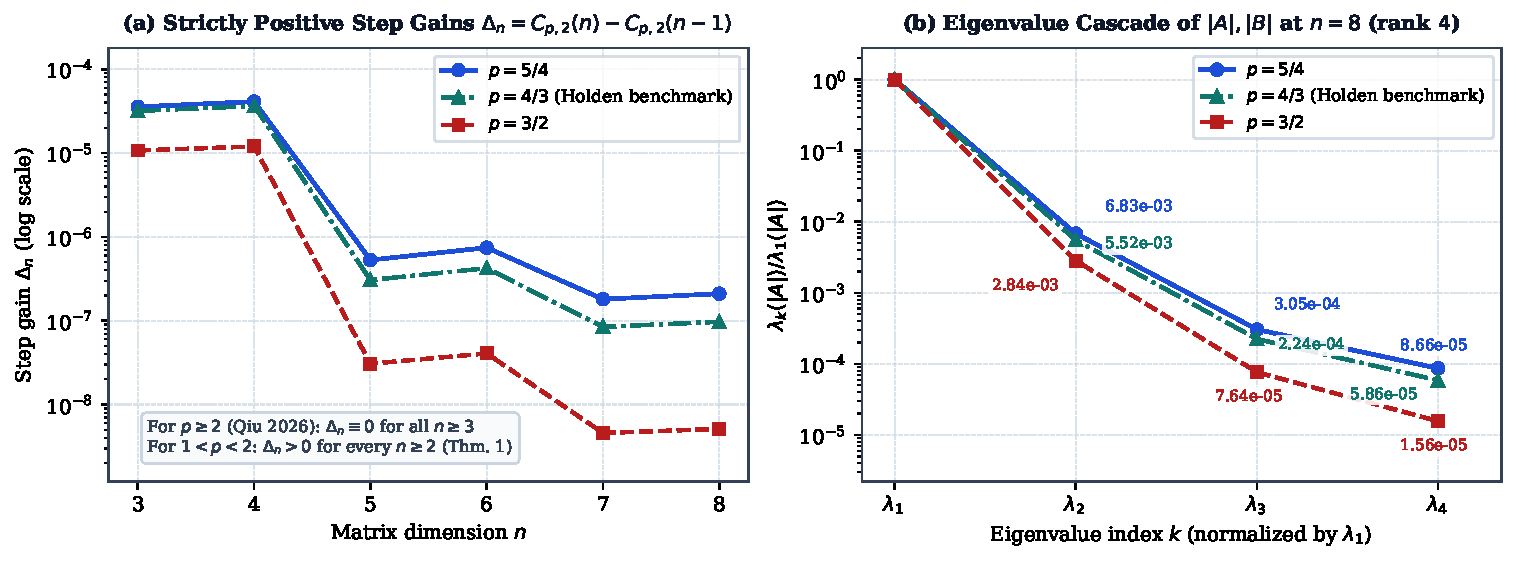
\includegraphics[width=0.98\textwidth]{fig1_staircase_cascade.pdf}
  \vspace{-6pt}
  \caption{\small \emph{Left (a):} Achieved dimensional step gains $\Delta_n = C_{p,2}(n) - C_{p,2}(n-1)$ across $n = 3,\dots,8$ for $p = 5/4$ (blue circles), $p = 4/3$ (teal triangles, Holden's benchmark exponent~\cite{Holden2026b}), and $p = 3/2$ (red squares), contrasting with $p \ge 2$ where $\Delta_n \equiv 0$ for all $n \ge 3$~\cite{Qiu2026}. Notice the paired odd/even plateau structure arising from the alternating rank growth $(1,1)\to(2,1)\to(2,2)\to\cdots$. \emph{Right (b):} Normalized nonzero eigenvalues of $|A|$ (matching $|B|$) at $n = 8$ (rank~$4$), showing rapid geometric decay.}
  \label{fig:cascade}
\end{figure}

\begin{table}[H]
\centering
\caption{\small Achieved lower-bound staircase for $C_{3/2,2}(n)$ across $n = 2,\dots,8$ (Tang--Zhang: $1.0346539519$; Holden interpolated upper bound~\cite{Holden2026b}: $1.04458345$; Theorem~6 $p_0=1, p_1=2$ bound: $1.06475224$).}
\vspace{3pt}
\footnotesize
\begin{tabular}{@{}c c l l l@{}}
\toprule
\textbf{Dim $n$} & \textbf{Ranks ($\rank A, \rank B$)} & \textbf{Achieved ratio} & \textbf{Step gain $\Delta_n$} & \textbf{Normalized nonzero eigenvalues of $|A|$} \\
\midrule
2 & $(1,1)$ & $1.03641435733341^*$ & $+3.641\times 10^{-2}$ & $[1.00]$ \\
3 & $(2,1)$ & $1.03642509117441$   & $+1.073\times 10^{-5}$ & $[1.00,\; 2.47\times 10^{-3}]$ \\
4 & $(2,2)$ & $1.03643708623764$   & $+1.200\times 10^{-5}$ & $[1.00,\; 2.79\times 10^{-3}]$ \\
5 & $(3,2)$ & $1.03643711693849$   & $+3.070\times 10^{-8}$ & $[1.00,\; 2.81\times 10^{-3},\; 5.46\times 10^{-5}]$ \\
6 & $(3,3)$ & $1.03643715767551$   & $+4.074\times 10^{-8}$ & $[1.00,\; 2.84\times 10^{-3},\; 7.63\times 10^{-5}]$ \\
7 & $(4,3)$ & $1.03643716225772$   & $+4.582\times 10^{-9}$ & $[1.00,\; 2.84\times 10^{-3},\; 7.63\times 10^{-5},\; 1.38\times 10^{-5}]$ \\
8 & $(4,4)$ & $1.03643716738222$   & $+5.125\times 10^{-9}$ & $[1.00,\; 2.84\times 10^{-3},\; 7.64\times 10^{-5},\; 1.56\times 10^{-5}]$ \\
\bottomrule
\end{tabular}
\label{tab:p32}
\end{table}

\begin{table}[H]
\centering
\caption{\small Achieved lower-bound staircase for $C_{4/3,2}(n)$ across $n = 2,\dots,8$ (Tang--Zhang: $1.0137583436$; Holden certified enclosure~\cite{Holden2026b}: $1.018371575 < C_{4/3,2}(\infty) \le (861/800)^{1/4} \approx 1.0185404735$).}
\vspace{3pt}
\footnotesize
\begin{tabular}{@{}c c l l l@{}}
\toprule
\textbf{Dim $n$} & \textbf{Ranks ($\rank A, \rank B$)} & \textbf{Achieved ratio} & \textbf{Step gain $\Delta_n$} & \textbf{Normalized nonzero eigenvalues of $|A|$} \\
\midrule
2 & $(1,1)$ & $1.01830237543067^*$ & $+1.830\times 10^{-2}$ & $[1.00]$ \\
3 & $(2,1)$ & $1.01833420141557$   & $+3.183\times 10^{-5}$ & $[1.00,\; 4.38\times 10^{-3}]$ \\
4 & $(2,2)$ & $1.01837064274052$   & $+3.644\times 10^{-5}$ & $[1.00,\; 5.19\times 10^{-3}]$ \\
5 & $(3,2)$ & $1.01837094872573$   & $+3.060\times 10^{-7}$ & $[1.00,\; 5.30\times 10^{-3},\; 1.43\times 10^{-4}]$ \\
6 & $(3,3)$ & $1.01837137193796$   & $+4.232\times 10^{-7}$ & $[1.00,\; 5.48\times 10^{-3},\; 2.22\times 10^{-4}]$ \\
7 & $(4,3)$ & $1.01837145645530$   & $+8.452\times 10^{-8}$ & $[1.00,\; 5.50\times 10^{-3},\; 2.23\times 10^{-4},\; 4.93\times 10^{-5}]$ \\
8 & $(4,4)$ & $1.01837155358673$   & $+9.713\times 10^{-8}$ & $[1.00,\; 5.52\times 10^{-3},\; 2.24\times 10^{-4},\; 5.86\times 10^{-5}]$ \\
\bottomrule
\end{tabular}
\label{tab:p43}
\end{table}

\begin{table}[H]
\centering
\caption{\small Achieved lower-bound staircase for $C_{5/4,2}(n)$ across $n = 2,\dots,8$ (Tang--Zhang: $1.0057587726$; Holden interpolated upper bound~\cite{Holden2026b}: $(861/800)^{1/5} \approx 1.01480508$; Theorem~19(a) pure-algebraic upper bound: $1.01252960$).}
\vspace{3pt}
\footnotesize
\begin{tabular}{@{}c c l l l@{}}
\toprule
\textbf{Dim $n$} & \textbf{Ranks ($\rank A, \rank B$)} & \textbf{Achieved ratio} & \textbf{Step gain $\Delta_n$} & \textbf{Normalized nonzero eigenvalues of $|A|$} \\
\midrule
2 & $(1,1)$ & $1.01098753445242^*$ & $+1.099\times 10^{-2}$ & $[1.00]$ \\
3 & $(2,1)$ & $1.01102311501737$   & $+3.558\times 10^{-5}$ & $[1.00,\; 5.11\times 10^{-3}]$ \\
4 & $(2,2)$ & $1.01106425559437$   & $+4.114\times 10^{-5}$ & $[1.00,\; 6.21\times 10^{-3}]$ \\
5 & $(3,2)$ & $1.01106478536413$   & $+5.298\times 10^{-7}$ & $[1.00,\; 6.41\times 10^{-3},\; 1.83\times 10^{-4}]$ \\
6 & $(3,3)$ & $1.01106552894231$   & $+7.436\times 10^{-7}$ & $[1.00,\; 6.74\times 10^{-3},\; 3.00\times 10^{-4}]$ \\
7 & $(4,3)$ & $1.01106570953544$   & $+1.806\times 10^{-7}$ & $[1.00,\; 6.78\times 10^{-3},\; 3.03\times 10^{-4},\; 7.09\times 10^{-5}]$ \\
8 & $(4,4)$ & $1.01106591970515$   & $+2.102\times 10^{-7}$ & $[1.00,\; 6.83\times 10^{-3},\; 3.05\times 10^{-4},\; 8.66\times 10^{-5}]$ \\
\bottomrule
\end{tabular}
\label{tab:p54}
\end{table}

\begin{table}[H]
\centering
\caption{\small Extended Theorem~5 PSD-formulation achieved lower-bound staircases ($W_k = Z_k Z_k^\top$, zero unitary variables; \texttt{investigate\_open\_core.py}) through $n = 14$ at $p = 3/2$ and $n = 12$ at $p = 4/3$, confirming pinned top density mass $\lambda_1(T)$ and exact orthogonal-projection defect $\|X_1^2 - X_1\|_F \approx 0$.}
\vspace{3pt}
\footnotesize
\begin{tabular}{@{}c c c l l c c c@{}}
\toprule
\textbf{Exp $p$} & \textbf{Dim $n$} & \textbf{Ranks} & \textbf{Achieved ratio} & \textbf{Even-step gain} & \textbf{Top $\lambda_1(T)$} & \textbf{Min $\lambda_n(T)$} & \textbf{$\|X_1^2 - X_1\|_F$} \\
\midrule
$3/2$ &  8 & $(4,4)$ & $1.036437167382224$ & $+9.707\times 10^{-9}$  & $0.987213$ & $2.20\times 10^{-9}$  & $9.6\times 10^{-12}$ \\
$3/2$ & 10 & $(5,5)$ & $1.036437167985572$ & $+6.033\times 10^{-10}$ & $0.987213$ & $2.12\times 10^{-10}$ & $1.8\times 10^{-11}$ \\
$3/2$ & 12 & $(6,6)$ & $1.036437168024622$ & $+3.905\times 10^{-11}$ & $0.987213$ & $8.86\times 10^{-12}$ & $5.8\times 10^{-10}$ \\
$3/2$ & 14 & $(7,7)$ & $1.036437168055158$ & $+3.054\times 10^{-11}$ & $0.987213$ & $8.62\times 10^{-12}$ & $4.9\times 10^{-9}$  \\
\midrule
$4/3$ &  8 & $(4,4)$ & $1.018371553586731$ & $+1.816\times 10^{-7}$  & $0.966815$ & $2.10\times 10^{-7}$  & $6.0\times 10^{-14}$ \\
$4/3$ & 10 & $(5,5)$ & $1.018371570141039$ & $+1.655\times 10^{-8}$  & $0.966808$ & $3.07\times 10^{-8}$  & $3.1\times 10^{-13}$ \\
$4/3$ & 12 & $(6,6)$ & $1.018371572808177$ & $+2.667\times 10^{-9}$  & $0.966807$ & $3.10\times 10^{-9}$  & $1.1\times 10^{-12}$ \\
\bottomrule
\end{tabular}
\label{tab:psd_ext}
\end{table}

\noindent{\footnotesize\textsuperscript{*}Exact analytical values from Theorem~3. For $m = 3$ at $p = 3/2$, Theorem~3 proves $C_{3/2,3}(2) = C_{3/2,2}(2) \approx 1.036414357333$, while exact-gradient optimization achieves strictly increasing ratios across $n = 2, 3, 4, 5$: $1.036414357333 < 1.063086305441 < 1.063090693728 < 1.063095357075$ (compare Tang--Zhang $C_{3/2,3}^{\TZ} \approx 1.0607584802$ and Theorem~17's zero-float upper bound $1.0633400433$). At $p = 4/3$, our $n = 12$ achieved ratio $1.0183715728$ approaches Holden's certified lower bound $1.018371575$~\cite{Holden2026b} from below, consistent with Holden's higher-order cyclic block construction and Theorem~1.}

\subsection{Open-Core Numerical Diagnostics (\texttt{investigate\_open\_core.py})}

Beyond verifying the extended staircases in Table~\ref{tab:psd_ext}, our numerical experiments probe the open structure of MI-20:
\begin{itemize}[leftmargin=1.5em,itemsep=2pt]
  \item \textbf{Continuous-spectrum Hardy/Toeplitz projection test:} Discretizing multiplication by a density $f(\theta) > 0$ on $\mathbb{T}$ with the Hardy projection $X_1 = P_+$ across $N \in \{32, 64, 128\}$ Fourier modes at $p = 3/2$ gives ratios $\le 1.0054$ (smooth cosine), $\le 1.0154$ (discontinuous step functions), and $\le 1.0297$ (localized spikes), decreasing monotonically with $N$. Direct 6-harmonic optimization at $N = 64$ peaks at $1.032629 < C_{3/2,2}(2) \approx 1.036414$. Together with the stabilized top eigenvalue $\lambda_1(T^{(n)}) \approx 0.987213$ ($p = 3/2$) and $0.966807$ ($p = 4/3$) in Table~\ref{tab:psd_ext} and Theorem~16's unconditional $\Sp$-attainment of $C_{p,m}^{\mathrm{tree}}(\infty)$, this provides strong evidence against total spectral vanishing.
  \item \textbf{$p \to 1^+$ quadratic scaling in higher dimensions (Theorems~10, 13, 18, 19, and~21):} Proposition~8 proves $\lim_{\varepsilon\to 0^+}(C_{1+\varepsilon,2}(2)-1)/\varepsilon^2 = c_2 \approx 0.21961442$. Optimizing $n = 4$ and $n = 6$ via Theorem~5 at $\varepsilon = 0.01$ achieves $(C_{1.01,2}(4)-1)/\varepsilon^2 = 0.223031$ and $(C_{1.01,2}(6)-1)/\varepsilon^2 = 0.223265$, approaching Theorem~18's 13-digit BCH tree constant $K_2^{\mathrm{tree}}(\infty) = 0.2259285429476\dots$, while Theorem~19(b) breaks Theorem~10's Lambert-$W$ barrier $0.317235793549\dots$ without Furuta down to $K_2^{\mathrm{BCH}} < 0.31722794$ and Theorem~21(c) pushes the unconditional bound $348.4\times$ further down to $K_2^{\mathrm{BCH}} < 0.3145$.
  \item \textbf{Dual-trace lower bound functional $\Tr(T^\alpha H) / \Tr(T)$:} By H\"older's inequality ($\alpha p' = 1$), $\|H\|_p \ge \Tr(T^\alpha H)$ holds in every dimension $n$ for Theorem~5's canonical form, so any uniform lower bound $\Tr(T^\alpha H) \ge \gamma_{p,m}\Tr(T)$ implies $C_{p,m}(\infty) \le \gamma_{p,m}^{-1}$. Numerically, for $m = 2$, $\min \Tr(T^\alpha H)/\Tr(T)$ stabilizes at $n = 2$ across $n \in \{2, 3, 4, 6\}$ for $p \in \{8/5, 3/2, 7/5\}$—attaining $\frac{2\sqrt{2}}{3} \approx 0.94280904$ at $p = 3/2$ ($1/\gamma = \frac{3\sqrt{2}}{4} \approx 1.060660$)—while breaking dimensional stabilization below $p \approx 4/3$ and maintaining $1 - \gamma_{p,2} \sim \Theta((p-1)^2)$ as $p \to 1^+$.
\end{itemize}

\subsection{Independent Zero-Float, 35/50-Digit, Symbolic, and 10-Line Verification}

All analytical identities, world-record lower bounds, Two-State Pinch upper bounds, continuous-interval multi-summand Bernstein records, full-V4-enclosure top-band splitting certificates, and BCH norm/upper bounds are independently reproduced by our bundled scripts:
\begin{itemize}[leftmargin=1.5em,itemsep=2pt]
  \item \textbf{Zero-float master certificate verifier (\texttt{python3 -B -S verify\_all\_exact\_certificates.py}, Suites~1--6):} Pure Python~3 standard library (\texttt{fractions}, \texttt{math}, \texttt{json}, \texttt{gzip}) with \textbf{zero floating-point literals or calls} (AST-audited) verifies all six suites in $84.9\,\mathrm{s}$ (Suites~1--4 in $0.3\,\mathrm{s}$, Suite~5 in $84.1\,\mathrm{s}$, Suite~6 in $0.50\,\mathrm{s}$): (1)~Theorem~4's three $2\times 3$ witnesses (Weyl radii $\epsilon_H < 1.5\times 10^{-39}$); (2)~Theorem~11's two $42\times 42$ world-record tree lower bounds (\texttt{lower\_record\_certificates.json}); (3)~Theorem~12's 18 four-corner Two-State Pinch convex-trapezoid certificates (\texttt{upper\_bound\_certificates.json}); (4)~four negative tamper regression tests plus a noncommuting matrix algebra sanity check; (5)~Theorem~17's four continuous-interval zero-float Bernstein multi-summand world records (\texttt{multisummand\_interval\_certs\_v5/}, 28 contiguous subintervals, literal \texttt{0/1} residuals across all $\delta^r$ powers, self-verified Bernstein basis conversion, exact rational Rump--Gershgorin strict PD, exact V4 Thm~10B/10C cap clearance, plus a Suite~5 tamper test); and (6)~Theorem~22(c)'s full-V4-enclosure top-band exact splitting certificates (\texttt{top\_band\_gap\_certs\_v5/\allowbreak p32\_iv\_patches.json}: 15 exact IV boxes at $p = 4/3$ in $0.01\,\mathrm{s}$, worst $c_0 \le -1.1307\times 10^{-4}$; 92 Krawczyk/centered-residual IV patches at $p = 3/2$ in $0.49\,\mathrm{s}$, $\min LDL^\top\text{ pivot} \ge 1.5\times 10^{-7}$, worst $c_0 \le -7.2735\times 10^{-4}$; plus a Suite~6 negative tamper test).
  \item \textbf{35-digit \texttt{mpmath.iv} BCH record \& norm-cap verifier (\texttt{uv run --with mpmath python3 verify\_\allowbreak bch\_\allowbreak theorems\_\allowbreak iv.py}):} Pure-\texttt{mpmath} (zero \texttt{numpy}/\texttt{scipy}/LP/SDP, strict outward interval rounding) verifies Theorem~21(b)--(c) in $11.0\,\mathrm{s}$: 2{,}037 adaptive \texttt{iv}-boxes + breakpoints + $[8,\infty)$ tail ($\le 0.298626$) certifying $K_2^{\mathrm{BCH}} < 0.3145$ ($\sup F \le 0.36425899 < 0.36426905 \le \sigma_{\lim}(0.3145)$, margin $\le -1.006\times 10^{-5}$), and 9 $t_+$-slices certifying $\|V\|_{\op} \le 13.412$ uniformly on $[0, 0.3172358]$ ($\le 11.390$ at $0.3172358$, $\le 10.619$ at $K_2^{\mathrm{tree}}(\infty)$).
  \item \textbf{50-digit Furuta-free BCH verifier (\texttt{uv run --with mpmath python3 verify\_bch\_closed\_form.py}):} Independently verifies every constant and inequality in Theorem~19(b) to 50 decimal digits in $< 1\,\mathrm{s}$ ($K_2^{\mathrm{BCH}} < 0.31722794 < 0.317235793549\dots$).
  \item \textbf{Symbolic and 105-digit audit (\texttt{verify\_all\_math.py}):} SymPy checks every derivative factorization, palindromic reduction, and Sturm uniqueness bound in Theorem~3 ($p \in \{3/2, 4/3, 5/4\}$); Lemma~4(a) passes $5{,}000$ random complex PSD matrices; Theorem~3's dual Cauchy--Schwarz bound passes $5{,}000$ random complex tuples; and Lemma~2 strictly increases $\|S\|_p$ on $100/100$ random rank-deficient tuples in 105-digit \texttt{mpmath}.
\end{itemize}

The following self-contained 10-line NumPy snippet reproduces Theorem~4(1) in under one second:
\begin{tcolorbox}[codebox]
\begin{lstlisting}
import numpy as np
p = 1.5
sp = lambda M: np.sum(np.linalg.svd(M, compute_uv=False)**p)**(1/p)
ab = lambda M: (lambda _, s, vt: (vt.T * s) @ vt)(*np.linalg.svd(M, full_matrices=False))
A = np.array([[49., 62., -1.], [11., 14., 0.], [0., 0., 0.]])
B = np.array([[81.,  0.,  0.], [ 0.,  0., 0.], [0., 0., 0.]])
C2 = ((107 + 51*np.sqrt(17)) / 256)**(1/6)  # exact 2x2 supremum (Theorem 3)
ratio = sp(A + B) / sp(ab(A) + ab(B))
print(f"2x2 supremum = {C2:.15f}\n3x3 integer  = {ratio:.15f}\ngap = {ratio - C2:+.3e}")
\end{lstlisting}
\end{tcolorbox}
\vspace{-2pt}
{\ttfamily\footnotesize\color{ink} Output: 2x2 supremum = 1.036414357333407 \;|\; 3x3 integer = 1.036415570430780 \;|\; gap = +1.213e-06.}

\section{Remaining Open Core and Exact Obstruction Analysis of Problem MI-20}\label{sec:open_core}

With Theorems~1--22, Propositions~5 and~8, the expanded Lean~4 formalization (Section~\ref{sec:lean}), and our zero-float Suites~1--6 and 35/50-digit BCH verifiers established—proving unconditional $(\Sp(\ell^2))^m$ attainment of $\Lambda_{\mathrm{tree}}(\infty)$ and Piece~1 $\implies$ Piece~2 at $p \in \{4/3, 3/2\}$ for all $m \ge 2$, closing all $2\times 2$ Master Trace inequalities analytically across $p = 4/3, 3/2$, and BCH, tightening certified $m = 3, 4$ upper bounds by $4.06\times$--$5.91\times$, improving $\mathcal{S}_{4/3}$ tree contraction $4\times$ to $\rho_4(s) < 1/8$, capping $\|V\|_{\op} \le 13.412$ and pushing $K_2^{\mathrm{BCH}} < 0.3145$ ($348.4\times$ tighter), and certifying non-compact top-band exact splitting across the full V4 enclosures—we now pinpoint the exact, sharply demarcated obstructions that keep Problem~MI-20 open:
\begin{enumerate}[leftmargin=1.6em,itemsep=3pt]
  \item \textbf{Closing the Master Trace Inequality at $s \ge 3$ (Sharpened Walls on Pinching, O1--O3 \& SOS Rank Growth):} While Theorem~20(a),(d) permanently closes $s \le 2$ (including O2 at $s = 2$) across $p = 4/3, 3/2$, and BCH, closing general $s \ge 3$ faces four decisive structural walls:
  \begin{itemize}[leftmargin=1.4em,itemsep=1.5pt]
    \item \emph{Refutation of naive pinching elimination:} On every $s$-tree block at $\Lambda > \Lambda_{k=1}$, $4\mathcal{W}_\Lambda(D_-, H_-) \le \Lambda(\sigma_+ + \sigma_-)d_1^4 < \frac{m}{m-1}\Lambda\sigma_+ d_1^4 = 4\mathcal{W}_\Lambda(D, H)$ analytically forces $4\mathcal{W}_\Lambda(D_+, H_+) - 2\Tr((B^*B)^2) > \Lambda(\frac{\sigma_+}{m-1} - \sigma_-) > 0$ (e.g., $+6.36\times 10^{-3}$ at $p = 4/3, m = 2$), so $P^+$ cannot be eliminated by dropping the positive-sector pinching remainder.
    \item \emph{(O1) Boundary crossings $0 \in \sigma(\Phi)$:} Theorem~20(d) reduces O1 with zero constraint qualification to proving $(\nabla^2_{xx} N)_{Z,Z} \prec 0$ on zero-flux modes $Z$; an analytic proof for general $s \ge 3$ remains open.
    \item \emph{(O2) Diagonal-subspace wall for $s \ge 3$:} Across all tested irreducible $s = 3$ solutions and $s = 2,\dots,8$ trees, $\nabla^2_{HH}\mathcal{S}_\Lambda$ exhibits zero folds and constant inertia $(s-, \frac{s(s-1)}{2}+)$; however, the $D$-diagonal block of $L_H$ becomes indefinite for $s \ge 6$ trees (e.g., $(5-, 3+)$ at $s = 8$), ruling out a naive diagonal/off-diagonal Sylvester proof and requiring a genuine Schur complement generalizing Theorem~20(d).
    \item \emph{(O3) Genuine strict local-maximum wall ($r \ge 2$):} At $p = 4/3$, $\Lambda = \Lambda_{\mathrm{tree}}(\infty)$, the irreducible $3\times 3$ 2-root bang-bang block $\phi = (-\tau, -\tau, +\sigma_+)$ ($\tau = 0.16100024 \ll \sigma_+ = 0.16172909$) has strictly negative definite reduced Hessian of $\mathcal{R}_\Lambda$ (eigenvalues $-155{,}678.7, -388.4$), proving $r \ge 2$ bang-bang blocks are \emph{genuine strict local maxima} requiring global comparison rather than local second-order criticality.
  \end{itemize}
  Furthermore, \emph{no finite polynomial degree $d$} in our 1-state tracial SOS hierarchy can reach zero gap (stretched-exponential eigenvalues force growing moment-matrix ranks $2, 6, 12, 14$ for $s = 2,\dots,5$), and $s \to s+1$ rank-1 Darboux updates are refuted ($\sigma_2/\sigma_1$ grows $0.03 \to 0.51$ in BCH and $0.002 \to 0.233$ at $p = 4/3$) because adding a branch globally re-equilibrates the stretched-exponential Nystr\"om mesh $r_i \sim 2\beta\sqrt{i}$ (despite strict eigenvalue interlacing and rank-2 Cauchy displacement $\sinh(\pi\Delta r/\phi_*)V$ with relative SVs $[1, 1, 10^{-6}]$).
  \item \textbf{Piece-1-Free Non-Vanishing (Open Piece~2 Frontier):} Theorem~22(d)'s irreducible $\mathbb{Z}/2N\mathbb{Z}$-ring and $\mathbb{Z}$-lattice counterexamples prove that \emph{no} argument using only Holden's first-order equations + irreducibility + $|\phi_{j,i}| \le \sigma_+(\Lambda)$ + top spectral gap can ever rule out total vanishing; any Piece-1-free proof of Open Piece~2 must use variational maximality (second-order optimality or global comparison). While Theorem~22(a) already refutes every $\mathbb{Z}/2N\mathbb{Z}$ ring, all $s \ge 5$ stars ($s = 4$ star already has $\lambda_+(H_{\mathrm{full}}) = +14.521$), depth-$\ge 2$ chains, equal-scale $2\times(\text{Star } s=4)$, 5-vertex 2-root bridges, and asymmetric 3- and 6-vertex bridges, and Theorem~22(c) splits the top band $(d_{\mathrm{gap}}, 1]$ unconditionally without compactness, closing Piece~2 independently of Piece~1 requires: (i)~generalizing Theorem~22(a)'s second-order exclusion to arbitrary $Z \ge 1$ and $\rank(P_B^-) \ge 2$ blocks on finite-$n$ global maximizers (forcing $R = 1, \beta_1 = 0$ via Theorem~22(b)); and (ii)~proving uniform Negative Trace Drift $\Tr(P_{\ge 0} D) \le \theta\Tr(P_- D)$ ($\theta < 1$) without Master-Trace saturation (noting perturbed-pencil root sums $\sum r_k < \Tr(P_{\ge 0} D)$ fail immediately above $\sigma_+$ near $r_{\max}$).
  \item \textbf{Spectral-Pencil Phase Boundary at $\kappa > 2$ ($1 < p < 4/3$) and All-$p$ Attainment:} By Theorem~16(d), all-$p$ tree attainment reduces solely to ruling out $\Tr(\Phi_{\mathrm{irr}}) = 0$ (equivalently proving $g'(1) \le 0$ where Theorem~14(d) proves $g''(t) > 0$). Any proof must essentially invoke $\ker(H - h_+ D) = \{0\}$ (as Theorem~16 does, since reducible $(D_2, H_2) \oplus N\cdot(1\times 1\ h_+)$ satisfies $\mathcal{W}_\Lambda \ge 0$ while violating $\rho_{2\kappa} < 1$), and the linear pencil deficit has an exact phase boundary at $\kappa = 2$, turning negative for $\kappa > 2$ as complex roots of $\widetilde{Q}_3(r)$ enter $\operatorname{Re}(r) < 0$.
  \item \textbf{Closing the $p \to 1^+$ BCH Gap $[0.2259285429476,\, 0.3145]$:} While Theorem~21(b)--(c) eliminates the unbounded $U$-ray obstruction ($\|V\|_{\op} \le 13.412$) and pushes $K_2^{\mathrm{BCH}} < 0.3145$ ($348.4\times$ past Theorem~19(b)), any relaxation enforcing the off-diagonal $\tanh\Delta/\Delta$ equation only on $S = [a, b]$ while keeping $\|A\|_{\op} \le 2/e$ on $S^c$ plateaus near $0.3144$ (matching our Archimedean-compact degree-3 SOS crossing near $0.3150$). Breaking past $0.314$ toward the tree limit $0.22592854$ will require coupling $\widetilde{\mathcal{T}}[V^2] = 2(1+t_+) V$ simultaneously across both $S$ and $S^c$, or extracting verified rational duals from degree $d_{\mathrm{half}} \ge 4$ compactified $(E, Q, W)$ SOS relaxations.
\end{enumerate}

\begin{thebibliography}{17}
\small
\bibitem{Lee2010}
E.-Y. Lee, \emph{Rotfel'd type inequalities for norms}, Linear Algebra and its Applications \textbf{433}(3) (2010), 580--584.

\bibitem{Lee2011}
E.-Y. Lee, \emph{Extension of Rotfel'd theorem}, Linear Algebra and its Applications \textbf{435}(4) (2011), 735--741.

\bibitem{LinZhang2022}
J. Lin and Y. Zhang, \emph{A proof of Lee's conjecture on the sum of absolute values of matrices}, Journal of Mathematical Analysis and Applications \textbf{516} (2022), 126542.

\bibitem{TangZhang2026}
Q. Tang and S. Zhang, \emph{Generalizing Lee's conjecture on the sum of absolute values of matrices}, Linear Algebra and its Applications \textbf{731} (2026), 196--204; arXiv:2510.16846.

\bibitem{Zeng2026}
Z. Zeng, H. Liu, and K. Ratnavelu, \emph{A counterexample to the Tang--Zhang Schatten norm conjecture and sharp positive results}, arXiv:2608.15558 (August 2026).

\bibitem{Qiu2026}
H. Qiu, \emph{Sharp quasi-reverse Minkowski inequality for Schatten norms}, arXiv:2608.17565v2 (August 2026).

\bibitem{Li2026}
X. Li, \emph{Sharp concave-function transfer for Lee-type Schatten norm inequalities}, arXiv:2608.25989v1 (August 2026).

\bibitem{Holden2026a}
S. Holden, \emph{MI-20: dual and projective normal forms}, audited partial-result note archived in \emph{Open Problems in Numerical Linear Algebra} (\nolinkurl{references/holden-matrix-2026-09-12/MI-20/result.md}), September 12, 2026.

\bibitem{Holden2026b}
S. Holden, \emph{MI-20, Round Four: An Exact Universal Bound and a Positive Power-System Reduction}, audited partial-result report archived in \emph{Open Problems in Numerical Linear Algebra} (\nolinkurl{references/holden-continuations-2026-09-13/MI-20/report.pdf}), September 13, 2026.

\bibitem{Davies1988}
E. B. Davies, \emph{Lipschitz continuity of functions of operators in the Schatten classes}, Journal of the London Mathematical Society \textbf{37}(1) (1988), 148--157.

\bibitem{OpenProblemsNLA}
A. Townsend et al., \emph{Open Problems in Numerical Linear Algebra (OpenProblemsInNLA)}, Problem MI-20: \emph{Sharp subquadratic Lee constants for sums of matrices}, \url{https://github.com/ajt60gaibb/OpenProblemsInNLA} (2026).

\bibitem{Furuta1987}
T. Furuta, \emph{$A \ge B \ge 0$ assures $(B^r A^p B^r)^{1/q} \ge B^{(p+2r)/q}$ for $r \ge 0$, $p \ge 0$, $q \ge 1$ with $(1+2r)q \ge p+2r$}, Proceedings of the American Mathematical Society \textbf{101}(1) (1987), 85--88.

\bibitem{Stahl2013}
H. R. Stahl, \emph{Proof of the BMV conjecture}, Acta Mathematica \textbf{211}(2) (2013), 255--290.

\bibitem{Bhatia1997}
R. Bhatia, \emph{Matrix Analysis}, Graduate Texts in Mathematics \textbf{169}, Springer, New York, 1997.

\bibitem{Kadison1952}
R. V. Kadison, \emph{A generalized Schwarz inequality and algebraic invariants for operator algebras}, Annals of Mathematics \textbf{56}(3) (1952), 494--503.

\bibitem{Rump2010}
S. M. Rump, \emph{Verification methods: Rigorous results using floating-point arithmetic}, Acta Numerica \textbf{19} (2010), 287--449.

\bibitem{FergusonBaileyArno1999}
H. R. P. Ferguson, D. H. Bailey, and S. Arno, \emph{Analysis of PSLQ, an integer relation finding algorithm}, Mathematics of Computation \textbf{68}(225) (1999), 351--369.
\end{thebibliography}

\end{document}
